\documentclass[twoside]{book}

% Packages required by doxygen
\usepackage{fixltx2e}
\usepackage{calc}
\usepackage{doxygen}
\usepackage[export]{adjustbox} % also loads graphicx
\usepackage{graphicx}
\usepackage[utf8]{inputenc}
\usepackage{makeidx}
\usepackage{multicol}
\usepackage{multirow}
\PassOptionsToPackage{warn}{textcomp}
\usepackage{textcomp}
\usepackage[nointegrals]{wasysym}
\usepackage[table]{xcolor}

% Font selection
\usepackage[T1]{fontenc}
\usepackage[scaled=.90]{helvet}
\usepackage{courier}
\usepackage{amssymb}
\usepackage{sectsty}
\renewcommand{\familydefault}{\sfdefault}
\allsectionsfont{%
  \fontseries{bc}\selectfont%
  \color{darkgray}%
}
\renewcommand{\DoxyLabelFont}{%
  \fontseries{bc}\selectfont%
  \color{darkgray}%
}
\newcommand{\+}{\discretionary{\mbox{\scriptsize$\hookleftarrow$}}{}{}}

% Page & text layout
\usepackage{geometry}
\geometry{%
  a4paper,%
  top=2.5cm,%
  bottom=2.5cm,%
  left=2.5cm,%
  right=2.5cm%
}
\tolerance=750
\hfuzz=15pt
\hbadness=750
\setlength{\emergencystretch}{15pt}
\setlength{\parindent}{0cm}
\setlength{\parskip}{3ex plus 2ex minus 2ex}
\makeatletter
\renewcommand{\paragraph}{%
  \@startsection{paragraph}{4}{0ex}{-1.0ex}{1.0ex}{%
    \normalfont\normalsize\bfseries\SS@parafont%
  }%
}
\renewcommand{\subparagraph}{%
  \@startsection{subparagraph}{5}{0ex}{-1.0ex}{1.0ex}{%
    \normalfont\normalsize\bfseries\SS@subparafont%
  }%
}
\makeatother

% Headers & footers
\usepackage{fancyhdr}
\pagestyle{fancyplain}
\fancyhead[LE]{\fancyplain{}{\bfseries\thepage}}
\fancyhead[CE]{\fancyplain{}{}}
\fancyhead[RE]{\fancyplain{}{\bfseries\leftmark}}
\fancyhead[LO]{\fancyplain{}{\bfseries\rightmark}}
\fancyhead[CO]{\fancyplain{}{}}
\fancyhead[RO]{\fancyplain{}{\bfseries\thepage}}
\fancyfoot[LE]{\fancyplain{}{}}
\fancyfoot[CE]{\fancyplain{}{}}
\fancyfoot[RE]{\fancyplain{}{\bfseries\scriptsize Generated by Doxygen }}
\fancyfoot[LO]{\fancyplain{}{\bfseries\scriptsize Generated by Doxygen }}
\fancyfoot[CO]{\fancyplain{}{}}
\fancyfoot[RO]{\fancyplain{}{}}
\renewcommand{\footrulewidth}{0.4pt}
\renewcommand{\chaptermark}[1]{%
  \markboth{#1}{}%
}
\renewcommand{\sectionmark}[1]{%
  \markright{\thesection\ #1}%
}

% Indices & bibliography
\usepackage{natbib}
\usepackage[titles]{tocloft}
\setcounter{tocdepth}{3}
\setcounter{secnumdepth}{5}
\makeindex

% Hyperlinks (required, but should be loaded last)
\usepackage{ifpdf}
\ifpdf
  \usepackage[pdftex,pagebackref=true]{hyperref}
\else
  \usepackage[ps2pdf,pagebackref=true]{hyperref}
\fi
\hypersetup{%
  colorlinks=true,%
  linkcolor=blue,%
  citecolor=blue,%
  unicode%
}

% Custom commands
\newcommand{\clearemptydoublepage}{%
  \newpage{\pagestyle{empty}\cleardoublepage}%
}

\usepackage{caption}
\captionsetup{labelsep=space,justification=centering,font={bf},singlelinecheck=off,skip=4pt,position=top}

%===== C O N T E N T S =====

\begin{document}

% Titlepage & ToC
\hypersetup{pageanchor=false,
             bookmarksnumbered=true,
             pdfencoding=unicode
            }
\pagenumbering{alph}
\begin{titlepage}
\vspace*{7cm}
\begin{center}%
{\Large My Project }\\
\vspace*{1cm}
{\large Generated by Doxygen 1.8.14}\\
\end{center}
\end{titlepage}
\clearemptydoublepage
\pagenumbering{roman}
\tableofcontents
\clearemptydoublepage
\pagenumbering{arabic}
\hypersetup{pageanchor=true}

%--- Begin generated contents ---
\chapter{Project Title}
\label{md__home_tetard_IdeaProjects_jCoinche_Java_jcoinche_2017_README}
\Hypertarget{md__home_tetard_IdeaProjects_jCoinche_Java_jcoinche_2017_README}
This is a school project in Java. The aim of the project was to learn Java programming language features by programming a network card Game. It\textquotesingle{}s a french game named \char`\"{}\+La belotte coinchée\char`\"{}.

For more informations about the game, see the official \href{http://www.beloteweb.eu/regles-de-la-belote-coinchee/}{\tt Belotte Coinchée Website}.

\subsection*{Getting Started}

To clone the repository\+: 
\begin{DoxyCode}
git clone git@git@epitech.eu:/girard\_z/Java\_jcoinche\_2017
cd Java\_jcoinche\_2017
\end{DoxyCode}


\subsubsection*{Prerequisites}

You should install \href{https://maven.apache.org/plugins/maven-compiler-plugin/index.html}{\tt Maven} and have at least the 8th version of \href{http://www.oracle.com/technetwork/java/javase/downloads/jdk8-downloads-2133151.html}{\tt Jdk}.

\subsubsection*{Installing}

First of all, install the dependencies and the environment\+:


\begin{DoxyCode}
mvn install
\end{DoxyCode}


Compile sources\+:


\begin{DoxyCode}
mvn compile
\end{DoxyCode}


Create packages\+: 
\begin{DoxyCode}
mvn package
\end{DoxyCode}


\subsubsection*{Running}


\begin{DoxyCode}
java -jar target/jcoinche-client.jar [ip address] [port]
java -jar target/jcoinche-server.jar [port]
\end{DoxyCode}


\subsection*{Documentation}

open {\ttfamily target/site/apidocs/index.\+html} or open {\ttfamily doxy/html/index.\+html}

\subsection*{Description}

The is a multiroom network game of coinche.

\subsubsection*{Rooms}

Each player is able to create/join a room. When four players are in a room, the party begins. When a player leaves a room / disconnect, the party is over and the room is waiting for a fourth player.

\subsubsection*{The Game}

When 4 players are ready in a room, the first player to be played can call.
\begin{DoxyItemize}
\item If nobody calls, cards are redistributed
\item if Somone Calls, the three next players have to skip there call to let the game begins.
\end{DoxyItemize}

\subsection*{The Commands}

you can type {\ttfamily help} to see the help.


\begin{DoxyCode}
help            ->      Helper
createroom      ->      Ask to create a room and join it if authorized
leave           ->      Ask to leave a room and leaves it if authorized 
disconnect      ->      Disconnect client
roomlist        ->      Show the list of rooms
join            ->      Try to join a room
ready           ->      Say to the room that you are ready to play
showmycards     ->      Display cards in your hands
call            ->      Make a call during the calling phase
\end{DoxyCode}


\subsection*{Built With}


\begin{DoxyItemize}
\item \href{https://maven.apache.org/}{\tt Maven} -\/ Dependency Management
\end{DoxyItemize}

\subsection*{Authors}


\begin{DoxyItemize}
\item {\bfseries Yohann N\textquotesingle{}Goala} -\/ {\itshape Software developer Front\+End} -\/ \href{https://github.com/YohannNgoala}{\tt Yoyo\+Le\+Ouf}
\item {\bfseries Benjamin Girard} -\/ {\itshape Software developer Back\+End} -\/ \href{https://github.com/BenjaminGirard}{\tt Têtard}
\end{DoxyItemize}

\subsection*{License}

This project is licensed under the E\+P\+I\+T\+E\+CH License. 
\chapter{Namespace Index}
\section{Namespace List}
Here is a list of all namespaces with brief descriptions\+:\begin{DoxyCompactList}
\item\contentsline{section}{\mbox{\hyperlink{namespaceClient}{Client}} }{\pageref{namespaceClient}}{}
\item\contentsline{section}{\mbox{\hyperlink{namespaceClient_1_1Model}{Client.\+Model}} }{\pageref{namespaceClient_1_1Model}}{}
\item\contentsline{section}{\mbox{\hyperlink{namespaceClient_1_1NetWork}{Client.\+Net\+Work}} }{\pageref{namespaceClient_1_1NetWork}}{}
\item\contentsline{section}{\mbox{\hyperlink{namespaceCommon}{Common}} }{\pageref{namespaceCommon}}{}
\item\contentsline{section}{\mbox{\hyperlink{namespaceServer}{Server}} }{\pageref{namespaceServer}}{}
\item\contentsline{section}{\mbox{\hyperlink{namespaceServer_1_1Game}{Server.\+Game}} }{\pageref{namespaceServer_1_1Game}}{}
\item\contentsline{section}{\mbox{\hyperlink{namespaceServer_1_1ServerConnexion}{Server.\+Server\+Connexion}} }{\pageref{namespaceServer_1_1ServerConnexion}}{}
\end{DoxyCompactList}

\chapter{Hierarchical Index}
\section{Class Hierarchy}
This inheritance list is sorted roughly, but not completely, alphabetically\+:\begin{DoxyCompactList}
\item \contentsline{section}{Client.\+Model.\+A\+Model}{\pageref{classClient_1_1Model_1_1AModel}}{}
\begin{DoxyCompactList}
\item \contentsline{section}{Client.\+Model.\+Instance\+Model}{\pageref{classClient_1_1Model_1_1InstanceModel}}{}
\item \contentsline{section}{Client.\+Model.\+Room\+List\+Model}{\pageref{classClient_1_1Model_1_1RoomListModel}}{}
\end{DoxyCompactList}
\item \contentsline{section}{Common.\+Are\+You\+Ready}{\pageref{classCommon_1_1AreYouReady}}{}
\item \contentsline{section}{Common.\+Ask\+Create\+Room}{\pageref{classCommon_1_1AskCreateRoom}}{}
\item \contentsline{section}{Common.\+Ask\+User\+Auth}{\pageref{classCommon_1_1AskUserAuth}}{}
\item \contentsline{section}{Common.\+Auth\+Answer}{\pageref{classCommon_1_1AuthAnswer}}{}
\item \contentsline{section}{Client.\+Binary\+Tree\+Rules}{\pageref{classClient_1_1BinaryTreeRules}}{}
\item \contentsline{section}{Common.\+Card}{\pageref{classCommon_1_1Card}}{}
\item \contentsline{section}{Common.\+Card\+Distributed}{\pageref{classCommon_1_1CardDistributed}}{}
\item \contentsline{section}{Common.\+Card\+Played}{\pageref{classCommon_1_1CardPlayed}}{}
\item \contentsline{section}{Client.\+Model.\+Card\+Printable}{\pageref{classClient_1_1Model_1_1CardPrintable}}{}
\item \contentsline{section}{Server.\+Game.\+Cards\+Values}{\pageref{classServer_1_1Game_1_1CardsValues}}{}
\item \contentsline{section}{Client.\+Net\+Work.\+Client\+Connection}{\pageref{classClient_1_1NetWork_1_1ClientConnection}}{}
\item \contentsline{section}{Server.\+Server\+Connexion.\+Client\+Infos}{\pageref{classServer_1_1ServerConnexion_1_1ClientInfos}}{}
\item \contentsline{section}{Common.\+Color}{\pageref{enumCommon_1_1Color}}{}
\item \contentsline{section}{Client.\+Controller}{\pageref{classClient_1_1Controller}}{}
\item \contentsline{section}{Server.\+Core}{\pageref{classServer_1_1Core}}{}
\item \contentsline{section}{Common.\+Game\+Cancelled}{\pageref{classCommon_1_1GameCancelled}}{}
\item \contentsline{section}{Server.\+Game.\+Game\+Infos}{\pageref{classServer_1_1Game_1_1GameInfos}}{}
\item \contentsline{section}{Server.\+Game.\+Game\+Master\+Coinche}{\pageref{classServer_1_1Game_1_1GameMasterCoinche}}{}
\item \contentsline{section}{Common.\+Game\+Over\+Points}{\pageref{classCommon_1_1GameOverPoints}}{}
\item \contentsline{section}{Common.\+I\+Am\+Ready}{\pageref{classCommon_1_1IAmReady}}{}
\item \contentsline{section}{Server.\+Server\+Connexion.\+I\+Server}{\pageref{interfaceServer_1_1ServerConnexion_1_1IServer}}{}
\begin{DoxyCompactList}
\item \contentsline{section}{Server.\+Server\+Connexion.\+Kryonet\+Server}{\pageref{classServer_1_1ServerConnexion_1_1KryonetServer}}{}
\end{DoxyCompactList}
\item \contentsline{section}{Common.\+Kryo\+Tool}{\pageref{classCommon_1_1KryoTool}}{}
\item \contentsline{section}{Client.\+Main}{\pageref{classClient_1_1Main}}{}
\item \contentsline{section}{Server.\+Main}{\pageref{classServer_1_1Main}}{}
\item \contentsline{section}{Client.\+Model.\+Other}{\pageref{classClient_1_1Model_1_1Other}}{}
\item \contentsline{section}{Common.\+Party\+Cancelled}{\pageref{classCommon_1_1PartyCancelled}}{}
\item \contentsline{section}{Common.\+Player}{\pageref{classCommon_1_1Player}}{}
\item \contentsline{section}{Common.\+Player\+Call\+Response}{\pageref{classCommon_1_1PlayerCallResponse}}{}
\item \contentsline{section}{Common.\+Player\+Ready}{\pageref{classCommon_1_1PlayerReady}}{}
\item \contentsline{section}{Client.\+Model.\+Ready\+State}{\pageref{enumClient_1_1Model_1_1ReadyState}}{}
\item \contentsline{section}{Server.\+Server\+Connexion.\+Request\+Handler}{\pageref{classServer_1_1ServerConnexion_1_1RequestHandler}}{}
\item \contentsline{section}{Server.\+Server\+Connexion.\+Room}{\pageref{classServer_1_1ServerConnexion_1_1Room}}{}
\item \contentsline{section}{Common.\+Room\+Access\+Answer}{\pageref{classCommon_1_1RoomAccessAnswer}}{}
\item \contentsline{section}{Common.\+Room\+Create}{\pageref{classCommon_1_1RoomCreate}}{}
\item \contentsline{section}{Common.\+Room\+Deleted}{\pageref{classCommon_1_1RoomDeleted}}{}
\item \contentsline{section}{Common.\+Room\+Info}{\pageref{classCommon_1_1RoomInfo}}{}
\item \contentsline{section}{Common.\+Room\+List\+Info}{\pageref{classCommon_1_1RoomListInfo}}{}
\item \contentsline{section}{Common.\+Room\+Moving\+Client}{\pageref{classCommon_1_1RoomMovingClient}}{}
\item \contentsline{section}{Client.\+Model.\+Score}{\pageref{classClient_1_1Model_1_1Score}}{}
\item \contentsline{section}{Common.\+Send\+Card\+To\+Player}{\pageref{classCommon_1_1SendCardToPlayer}}{}
\item \contentsline{section}{Common.\+Team\+Attribution}{\pageref{classCommon_1_1TeamAttribution}}{}
\item \contentsline{section}{Common.\+Trump}{\pageref{enumCommon_1_1Trump}}{}
\item \contentsline{section}{Common.\+Turn\+Over}{\pageref{classCommon_1_1TurnOver}}{}
\item \contentsline{section}{Common.\+Your\+Turn\+Call}{\pageref{classCommon_1_1YourTurnCall}}{}
\item \contentsline{section}{Common.\+Your\+Turn\+Play\+Card}{\pageref{classCommon_1_1YourTurnPlayCard}}{}
\end{DoxyCompactList}

\chapter{Class Index}
\section{Class List}
Here are the classes, structs, unions and interfaces with brief descriptions\+:\begin{DoxyCompactList}
\item\contentsline{section}{\mbox{\hyperlink{classClient_1_1Model_1_1AModel}{Client.\+Model.\+A\+Model}} }{\pageref{classClient_1_1Model_1_1AModel}}{}
\item\contentsline{section}{\mbox{\hyperlink{classCommon_1_1AreYouReady}{Common.\+Are\+You\+Ready}} }{\pageref{classCommon_1_1AreYouReady}}{}
\item\contentsline{section}{\mbox{\hyperlink{classCommon_1_1AskCreateRoom}{Common.\+Ask\+Create\+Room}} }{\pageref{classCommon_1_1AskCreateRoom}}{}
\item\contentsline{section}{\mbox{\hyperlink{classCommon_1_1AskUserAuth}{Common.\+Ask\+User\+Auth}} }{\pageref{classCommon_1_1AskUserAuth}}{}
\item\contentsline{section}{\mbox{\hyperlink{classCommon_1_1AuthAnswer}{Common.\+Auth\+Answer}} }{\pageref{classCommon_1_1AuthAnswer}}{}
\item\contentsline{section}{\mbox{\hyperlink{classClient_1_1BinaryTreeRules}{Client.\+Binary\+Tree\+Rules}} }{\pageref{classClient_1_1BinaryTreeRules}}{}
\item\contentsline{section}{\mbox{\hyperlink{classCommon_1_1Card}{Common.\+Card}} }{\pageref{classCommon_1_1Card}}{}
\item\contentsline{section}{\mbox{\hyperlink{classCommon_1_1CardDistributed}{Common.\+Card\+Distributed}} }{\pageref{classCommon_1_1CardDistributed}}{}
\item\contentsline{section}{\mbox{\hyperlink{classCommon_1_1CardPlayed}{Common.\+Card\+Played}} }{\pageref{classCommon_1_1CardPlayed}}{}
\item\contentsline{section}{\mbox{\hyperlink{classClient_1_1Model_1_1CardPrintable}{Client.\+Model.\+Card\+Printable}} }{\pageref{classClient_1_1Model_1_1CardPrintable}}{}
\item\contentsline{section}{\mbox{\hyperlink{classServer_1_1Game_1_1CardsValues}{Server.\+Game.\+Cards\+Values}} }{\pageref{classServer_1_1Game_1_1CardsValues}}{}
\item\contentsline{section}{\mbox{\hyperlink{classClient_1_1NetWork_1_1ClientConnection}{Client.\+Net\+Work.\+Client\+Connection}} }{\pageref{classClient_1_1NetWork_1_1ClientConnection}}{}
\item\contentsline{section}{\mbox{\hyperlink{classServer_1_1ServerConnexion_1_1ClientInfos}{Server.\+Server\+Connexion.\+Client\+Infos}} }{\pageref{classServer_1_1ServerConnexion_1_1ClientInfos}}{}
\item\contentsline{section}{\mbox{\hyperlink{enumCommon_1_1Color}{Common.\+Color}} }{\pageref{enumCommon_1_1Color}}{}
\item\contentsline{section}{\mbox{\hyperlink{classClient_1_1Controller}{Client.\+Controller}} }{\pageref{classClient_1_1Controller}}{}
\item\contentsline{section}{\mbox{\hyperlink{classServer_1_1Core}{Server.\+Core}} }{\pageref{classServer_1_1Core}}{}
\item\contentsline{section}{\mbox{\hyperlink{classCommon_1_1GameCancelled}{Common.\+Game\+Cancelled}} }{\pageref{classCommon_1_1GameCancelled}}{}
\item\contentsline{section}{\mbox{\hyperlink{classServer_1_1Game_1_1GameInfos}{Server.\+Game.\+Game\+Infos}} }{\pageref{classServer_1_1Game_1_1GameInfos}}{}
\item\contentsline{section}{\mbox{\hyperlink{classServer_1_1Game_1_1GameMasterCoinche}{Server.\+Game.\+Game\+Master\+Coinche}} }{\pageref{classServer_1_1Game_1_1GameMasterCoinche}}{}
\item\contentsline{section}{\mbox{\hyperlink{classCommon_1_1GameOverPoints}{Common.\+Game\+Over\+Points}} }{\pageref{classCommon_1_1GameOverPoints}}{}
\item\contentsline{section}{\mbox{\hyperlink{classCommon_1_1IAmReady}{Common.\+I\+Am\+Ready}} }{\pageref{classCommon_1_1IAmReady}}{}
\item\contentsline{section}{\mbox{\hyperlink{classClient_1_1Model_1_1InstanceModel}{Client.\+Model.\+Instance\+Model}} }{\pageref{classClient_1_1Model_1_1InstanceModel}}{}
\item\contentsline{section}{\mbox{\hyperlink{interfaceServer_1_1ServerConnexion_1_1IServer}{Server.\+Server\+Connexion.\+I\+Server}} }{\pageref{interfaceServer_1_1ServerConnexion_1_1IServer}}{}
\item\contentsline{section}{\mbox{\hyperlink{classServer_1_1ServerConnexion_1_1KryonetServer}{Server.\+Server\+Connexion.\+Kryonet\+Server}} }{\pageref{classServer_1_1ServerConnexion_1_1KryonetServer}}{}
\item\contentsline{section}{\mbox{\hyperlink{classCommon_1_1KryoTool}{Common.\+Kryo\+Tool}} }{\pageref{classCommon_1_1KryoTool}}{}
\item\contentsline{section}{\mbox{\hyperlink{classClient_1_1Main}{Client.\+Main}} }{\pageref{classClient_1_1Main}}{}
\item\contentsline{section}{\mbox{\hyperlink{classServer_1_1Main}{Server.\+Main}} }{\pageref{classServer_1_1Main}}{}
\item\contentsline{section}{\mbox{\hyperlink{classClient_1_1Model_1_1Other}{Client.\+Model.\+Other}} }{\pageref{classClient_1_1Model_1_1Other}}{}
\item\contentsline{section}{\mbox{\hyperlink{classCommon_1_1PartyCancelled}{Common.\+Party\+Cancelled}} }{\pageref{classCommon_1_1PartyCancelled}}{}
\item\contentsline{section}{\mbox{\hyperlink{classCommon_1_1Player}{Common.\+Player}} }{\pageref{classCommon_1_1Player}}{}
\item\contentsline{section}{\mbox{\hyperlink{classCommon_1_1PlayerCallResponse}{Common.\+Player\+Call\+Response}} }{\pageref{classCommon_1_1PlayerCallResponse}}{}
\item\contentsline{section}{\mbox{\hyperlink{classCommon_1_1PlayerReady}{Common.\+Player\+Ready}} }{\pageref{classCommon_1_1PlayerReady}}{}
\item\contentsline{section}{\mbox{\hyperlink{enumClient_1_1Model_1_1ReadyState}{Client.\+Model.\+Ready\+State}} }{\pageref{enumClient_1_1Model_1_1ReadyState}}{}
\item\contentsline{section}{\mbox{\hyperlink{classServer_1_1ServerConnexion_1_1RequestHandler}{Server.\+Server\+Connexion.\+Request\+Handler}} }{\pageref{classServer_1_1ServerConnexion_1_1RequestHandler}}{}
\item\contentsline{section}{\mbox{\hyperlink{classServer_1_1ServerConnexion_1_1Room}{Server.\+Server\+Connexion.\+Room}} }{\pageref{classServer_1_1ServerConnexion_1_1Room}}{}
\item\contentsline{section}{\mbox{\hyperlink{classCommon_1_1RoomAccessAnswer}{Common.\+Room\+Access\+Answer}} }{\pageref{classCommon_1_1RoomAccessAnswer}}{}
\item\contentsline{section}{\mbox{\hyperlink{classCommon_1_1RoomCreate}{Common.\+Room\+Create}} }{\pageref{classCommon_1_1RoomCreate}}{}
\item\contentsline{section}{\mbox{\hyperlink{classCommon_1_1RoomDeleted}{Common.\+Room\+Deleted}} }{\pageref{classCommon_1_1RoomDeleted}}{}
\item\contentsline{section}{\mbox{\hyperlink{classCommon_1_1RoomInfo}{Common.\+Room\+Info}} }{\pageref{classCommon_1_1RoomInfo}}{}
\item\contentsline{section}{\mbox{\hyperlink{classCommon_1_1RoomListInfo}{Common.\+Room\+List\+Info}} }{\pageref{classCommon_1_1RoomListInfo}}{}
\item\contentsline{section}{\mbox{\hyperlink{classClient_1_1Model_1_1RoomListModel}{Client.\+Model.\+Room\+List\+Model}} }{\pageref{classClient_1_1Model_1_1RoomListModel}}{}
\item\contentsline{section}{\mbox{\hyperlink{classCommon_1_1RoomMovingClient}{Common.\+Room\+Moving\+Client}} }{\pageref{classCommon_1_1RoomMovingClient}}{}
\item\contentsline{section}{\mbox{\hyperlink{classClient_1_1Model_1_1Score}{Client.\+Model.\+Score}} }{\pageref{classClient_1_1Model_1_1Score}}{}
\item\contentsline{section}{\mbox{\hyperlink{classCommon_1_1SendCardToPlayer}{Common.\+Send\+Card\+To\+Player}} }{\pageref{classCommon_1_1SendCardToPlayer}}{}
\item\contentsline{section}{\mbox{\hyperlink{classCommon_1_1TeamAttribution}{Common.\+Team\+Attribution}} }{\pageref{classCommon_1_1TeamAttribution}}{}
\item\contentsline{section}{\mbox{\hyperlink{enumCommon_1_1Trump}{Common.\+Trump}} }{\pageref{enumCommon_1_1Trump}}{}
\item\contentsline{section}{\mbox{\hyperlink{classCommon_1_1TurnOver}{Common.\+Turn\+Over}} }{\pageref{classCommon_1_1TurnOver}}{}
\item\contentsline{section}{\mbox{\hyperlink{classCommon_1_1YourTurnCall}{Common.\+Your\+Turn\+Call}} }{\pageref{classCommon_1_1YourTurnCall}}{}
\item\contentsline{section}{\mbox{\hyperlink{classCommon_1_1YourTurnPlayCard}{Common.\+Your\+Turn\+Play\+Card}} }{\pageref{classCommon_1_1YourTurnPlayCard}}{}
\end{DoxyCompactList}

\chapter{File Index}
\section{File List}
Here is a list of all files with brief descriptions\+:\begin{DoxyCompactList}
\item\contentsline{section}{/home/tetard/\+Idea\+Projects/j\+Coinche/\+Java\+\_\+jcoinche\+\_\+2017/src/main/java/\+Client/\mbox{\hyperlink{BinaryTreeRules_8java}{Binary\+Tree\+Rules.\+java}} }{\pageref{BinaryTreeRules_8java}}{}
\item\contentsline{section}{/home/tetard/\+Idea\+Projects/j\+Coinche/\+Java\+\_\+jcoinche\+\_\+2017/src/main/java/\+Client/\mbox{\hyperlink{Controller_8java}{Controller.\+java}} }{\pageref{Controller_8java}}{}
\item\contentsline{section}{/home/tetard/\+Idea\+Projects/j\+Coinche/\+Java\+\_\+jcoinche\+\_\+2017/src/main/java/\+Client/\mbox{\hyperlink{Client_2Main_8java}{Main.\+java}} }{\pageref{Client_2Main_8java}}{}
\item\contentsline{section}{/home/tetard/\+Idea\+Projects/j\+Coinche/\+Java\+\_\+jcoinche\+\_\+2017/src/main/java/\+Client/\+Model/\mbox{\hyperlink{AModel_8java}{A\+Model.\+java}} }{\pageref{AModel_8java}}{}
\item\contentsline{section}{/home/tetard/\+Idea\+Projects/j\+Coinche/\+Java\+\_\+jcoinche\+\_\+2017/src/main/java/\+Client/\+Model/\mbox{\hyperlink{CardPrintable_8java}{Card\+Printable.\+java}} }{\pageref{CardPrintable_8java}}{}
\item\contentsline{section}{/home/tetard/\+Idea\+Projects/j\+Coinche/\+Java\+\_\+jcoinche\+\_\+2017/src/main/java/\+Client/\+Model/\mbox{\hyperlink{InstanceModel_8java}{Instance\+Model.\+java}} }{\pageref{InstanceModel_8java}}{}
\item\contentsline{section}{/home/tetard/\+Idea\+Projects/j\+Coinche/\+Java\+\_\+jcoinche\+\_\+2017/src/main/java/\+Client/\+Model/\mbox{\hyperlink{Other_8java}{Other.\+java}} }{\pageref{Other_8java}}{}
\item\contentsline{section}{/home/tetard/\+Idea\+Projects/j\+Coinche/\+Java\+\_\+jcoinche\+\_\+2017/src/main/java/\+Client/\+Model/\mbox{\hyperlink{ReadyState_8java}{Ready\+State.\+java}} }{\pageref{ReadyState_8java}}{}
\item\contentsline{section}{/home/tetard/\+Idea\+Projects/j\+Coinche/\+Java\+\_\+jcoinche\+\_\+2017/src/main/java/\+Client/\+Model/\mbox{\hyperlink{RoomListModel_8java}{Room\+List\+Model.\+java}} }{\pageref{RoomListModel_8java}}{}
\item\contentsline{section}{/home/tetard/\+Idea\+Projects/j\+Coinche/\+Java\+\_\+jcoinche\+\_\+2017/src/main/java/\+Client/\+Model/\mbox{\hyperlink{Score_8java}{Score.\+java}} }{\pageref{Score_8java}}{}
\item\contentsline{section}{/home/tetard/\+Idea\+Projects/j\+Coinche/\+Java\+\_\+jcoinche\+\_\+2017/src/main/java/\+Client/\+Net\+Work/\mbox{\hyperlink{ClientConnection_8java}{Client\+Connection.\+java}} }{\pageref{ClientConnection_8java}}{}
\item\contentsline{section}{/home/tetard/\+Idea\+Projects/j\+Coinche/\+Java\+\_\+jcoinche\+\_\+2017/src/main/java/\+Common/\mbox{\hyperlink{AreYouReady_8java}{Are\+You\+Ready.\+java}} }{\pageref{AreYouReady_8java}}{}
\item\contentsline{section}{/home/tetard/\+Idea\+Projects/j\+Coinche/\+Java\+\_\+jcoinche\+\_\+2017/src/main/java/\+Common/\mbox{\hyperlink{AskCreateRoom_8java}{Ask\+Create\+Room.\+java}} }{\pageref{AskCreateRoom_8java}}{}
\item\contentsline{section}{/home/tetard/\+Idea\+Projects/j\+Coinche/\+Java\+\_\+jcoinche\+\_\+2017/src/main/java/\+Common/\mbox{\hyperlink{AskUserAuth_8java}{Ask\+User\+Auth.\+java}} }{\pageref{AskUserAuth_8java}}{}
\item\contentsline{section}{/home/tetard/\+Idea\+Projects/j\+Coinche/\+Java\+\_\+jcoinche\+\_\+2017/src/main/java/\+Common/\mbox{\hyperlink{AuthAnswer_8java}{Auth\+Answer.\+java}} }{\pageref{AuthAnswer_8java}}{}
\item\contentsline{section}{/home/tetard/\+Idea\+Projects/j\+Coinche/\+Java\+\_\+jcoinche\+\_\+2017/src/main/java/\+Common/\mbox{\hyperlink{Card_8java}{Card.\+java}} }{\pageref{Card_8java}}{}
\item\contentsline{section}{/home/tetard/\+Idea\+Projects/j\+Coinche/\+Java\+\_\+jcoinche\+\_\+2017/src/main/java/\+Common/\mbox{\hyperlink{CardDistributed_8java}{Card\+Distributed.\+java}} }{\pageref{CardDistributed_8java}}{}
\item\contentsline{section}{/home/tetard/\+Idea\+Projects/j\+Coinche/\+Java\+\_\+jcoinche\+\_\+2017/src/main/java/\+Common/\mbox{\hyperlink{CardPlayed_8java}{Card\+Played.\+java}} }{\pageref{CardPlayed_8java}}{}
\item\contentsline{section}{/home/tetard/\+Idea\+Projects/j\+Coinche/\+Java\+\_\+jcoinche\+\_\+2017/src/main/java/\+Common/\mbox{\hyperlink{Color_8java}{Color.\+java}} }{\pageref{Color_8java}}{}
\item\contentsline{section}{/home/tetard/\+Idea\+Projects/j\+Coinche/\+Java\+\_\+jcoinche\+\_\+2017/src/main/java/\+Common/\mbox{\hyperlink{GameCancelled_8java}{Game\+Cancelled.\+java}} }{\pageref{GameCancelled_8java}}{}
\item\contentsline{section}{/home/tetard/\+Idea\+Projects/j\+Coinche/\+Java\+\_\+jcoinche\+\_\+2017/src/main/java/\+Common/\mbox{\hyperlink{GameOverPoints_8java}{Game\+Over\+Points.\+java}} }{\pageref{GameOverPoints_8java}}{}
\item\contentsline{section}{/home/tetard/\+Idea\+Projects/j\+Coinche/\+Java\+\_\+jcoinche\+\_\+2017/src/main/java/\+Common/\mbox{\hyperlink{IAmReady_8java}{I\+Am\+Ready.\+java}} }{\pageref{IAmReady_8java}}{}
\item\contentsline{section}{/home/tetard/\+Idea\+Projects/j\+Coinche/\+Java\+\_\+jcoinche\+\_\+2017/src/main/java/\+Common/\mbox{\hyperlink{KryoTool_8java}{Kryo\+Tool.\+java}} }{\pageref{KryoTool_8java}}{}
\item\contentsline{section}{/home/tetard/\+Idea\+Projects/j\+Coinche/\+Java\+\_\+jcoinche\+\_\+2017/src/main/java/\+Common/\mbox{\hyperlink{PartyCancelled_8java}{Party\+Cancelled.\+java}} }{\pageref{PartyCancelled_8java}}{}
\item\contentsline{section}{/home/tetard/\+Idea\+Projects/j\+Coinche/\+Java\+\_\+jcoinche\+\_\+2017/src/main/java/\+Common/\mbox{\hyperlink{Player_8java}{Player.\+java}} }{\pageref{Player_8java}}{}
\item\contentsline{section}{/home/tetard/\+Idea\+Projects/j\+Coinche/\+Java\+\_\+jcoinche\+\_\+2017/src/main/java/\+Common/\mbox{\hyperlink{PlayerCallResponse_8java}{Player\+Call\+Response.\+java}} }{\pageref{PlayerCallResponse_8java}}{}
\item\contentsline{section}{/home/tetard/\+Idea\+Projects/j\+Coinche/\+Java\+\_\+jcoinche\+\_\+2017/src/main/java/\+Common/\mbox{\hyperlink{PlayerReady_8java}{Player\+Ready.\+java}} }{\pageref{PlayerReady_8java}}{}
\item\contentsline{section}{/home/tetard/\+Idea\+Projects/j\+Coinche/\+Java\+\_\+jcoinche\+\_\+2017/src/main/java/\+Common/\mbox{\hyperlink{RoomAccessAnswer_8java}{Room\+Access\+Answer.\+java}} }{\pageref{RoomAccessAnswer_8java}}{}
\item\contentsline{section}{/home/tetard/\+Idea\+Projects/j\+Coinche/\+Java\+\_\+jcoinche\+\_\+2017/src/main/java/\+Common/\mbox{\hyperlink{RoomCreate_8java}{Room\+Create.\+java}} }{\pageref{RoomCreate_8java}}{}
\item\contentsline{section}{/home/tetard/\+Idea\+Projects/j\+Coinche/\+Java\+\_\+jcoinche\+\_\+2017/src/main/java/\+Common/\mbox{\hyperlink{RoomDeleted_8java}{Room\+Deleted.\+java}} }{\pageref{RoomDeleted_8java}}{}
\item\contentsline{section}{/home/tetard/\+Idea\+Projects/j\+Coinche/\+Java\+\_\+jcoinche\+\_\+2017/src/main/java/\+Common/\mbox{\hyperlink{RoomInfo_8java}{Room\+Info.\+java}} }{\pageref{RoomInfo_8java}}{}
\item\contentsline{section}{/home/tetard/\+Idea\+Projects/j\+Coinche/\+Java\+\_\+jcoinche\+\_\+2017/src/main/java/\+Common/\mbox{\hyperlink{RoomListInfo_8java}{Room\+List\+Info.\+java}} }{\pageref{RoomListInfo_8java}}{}
\item\contentsline{section}{/home/tetard/\+Idea\+Projects/j\+Coinche/\+Java\+\_\+jcoinche\+\_\+2017/src/main/java/\+Common/\mbox{\hyperlink{RoomMovingClient_8java}{Room\+Moving\+Client.\+java}} }{\pageref{RoomMovingClient_8java}}{}
\item\contentsline{section}{/home/tetard/\+Idea\+Projects/j\+Coinche/\+Java\+\_\+jcoinche\+\_\+2017/src/main/java/\+Common/\mbox{\hyperlink{SendCardToPlayer_8java}{Send\+Card\+To\+Player.\+java}} }{\pageref{SendCardToPlayer_8java}}{}
\item\contentsline{section}{/home/tetard/\+Idea\+Projects/j\+Coinche/\+Java\+\_\+jcoinche\+\_\+2017/src/main/java/\+Common/\mbox{\hyperlink{TeamAttribution_8java}{Team\+Attribution.\+java}} }{\pageref{TeamAttribution_8java}}{}
\item\contentsline{section}{/home/tetard/\+Idea\+Projects/j\+Coinche/\+Java\+\_\+jcoinche\+\_\+2017/src/main/java/\+Common/\mbox{\hyperlink{Trump_8java}{Trump.\+java}} }{\pageref{Trump_8java}}{}
\item\contentsline{section}{/home/tetard/\+Idea\+Projects/j\+Coinche/\+Java\+\_\+jcoinche\+\_\+2017/src/main/java/\+Common/\mbox{\hyperlink{TurnOver_8java}{Turn\+Over.\+java}} }{\pageref{TurnOver_8java}}{}
\item\contentsline{section}{/home/tetard/\+Idea\+Projects/j\+Coinche/\+Java\+\_\+jcoinche\+\_\+2017/src/main/java/\+Common/\mbox{\hyperlink{YourTurnCall_8java}{Your\+Turn\+Call.\+java}} }{\pageref{YourTurnCall_8java}}{}
\item\contentsline{section}{/home/tetard/\+Idea\+Projects/j\+Coinche/\+Java\+\_\+jcoinche\+\_\+2017/src/main/java/\+Common/\mbox{\hyperlink{YourTurnPlayCard_8java}{Your\+Turn\+Play\+Card.\+java}} }{\pageref{YourTurnPlayCard_8java}}{}
\item\contentsline{section}{/home/tetard/\+Idea\+Projects/j\+Coinche/\+Java\+\_\+jcoinche\+\_\+2017/src/main/java/\+Server/\mbox{\hyperlink{Core_8java}{Core.\+java}} }{\pageref{Core_8java}}{}
\item\contentsline{section}{/home/tetard/\+Idea\+Projects/j\+Coinche/\+Java\+\_\+jcoinche\+\_\+2017/src/main/java/\+Server/\mbox{\hyperlink{Server_2Main_8java}{Main.\+java}} }{\pageref{Server_2Main_8java}}{}
\item\contentsline{section}{/home/tetard/\+Idea\+Projects/j\+Coinche/\+Java\+\_\+jcoinche\+\_\+2017/src/main/java/\+Server/\+Game/\mbox{\hyperlink{CardsValues_8java}{Cards\+Values.\+java}} }{\pageref{CardsValues_8java}}{}
\item\contentsline{section}{/home/tetard/\+Idea\+Projects/j\+Coinche/\+Java\+\_\+jcoinche\+\_\+2017/src/main/java/\+Server/\+Game/\mbox{\hyperlink{GameInfos_8java}{Game\+Infos.\+java}} }{\pageref{GameInfos_8java}}{}
\item\contentsline{section}{/home/tetard/\+Idea\+Projects/j\+Coinche/\+Java\+\_\+jcoinche\+\_\+2017/src/main/java/\+Server/\+Game/\mbox{\hyperlink{GameMasterCoinche_8java}{Game\+Master\+Coinche.\+java}} }{\pageref{GameMasterCoinche_8java}}{}
\item\contentsline{section}{/home/tetard/\+Idea\+Projects/j\+Coinche/\+Java\+\_\+jcoinche\+\_\+2017/src/main/java/\+Server/\+Server\+Connexion/\mbox{\hyperlink{ClientInfos_8java}{Client\+Infos.\+java}} }{\pageref{ClientInfos_8java}}{}
\item\contentsline{section}{/home/tetard/\+Idea\+Projects/j\+Coinche/\+Java\+\_\+jcoinche\+\_\+2017/src/main/java/\+Server/\+Server\+Connexion/\mbox{\hyperlink{IServer_8java}{I\+Server.\+java}} }{\pageref{IServer_8java}}{}
\item\contentsline{section}{/home/tetard/\+Idea\+Projects/j\+Coinche/\+Java\+\_\+jcoinche\+\_\+2017/src/main/java/\+Server/\+Server\+Connexion/\mbox{\hyperlink{KryonetServer_8java}{Kryonet\+Server.\+java}} }{\pageref{KryonetServer_8java}}{}
\item\contentsline{section}{/home/tetard/\+Idea\+Projects/j\+Coinche/\+Java\+\_\+jcoinche\+\_\+2017/src/main/java/\+Server/\+Server\+Connexion/\mbox{\hyperlink{RequestHandler_8java}{Request\+Handler.\+java}} }{\pageref{RequestHandler_8java}}{}
\item\contentsline{section}{/home/tetard/\+Idea\+Projects/j\+Coinche/\+Java\+\_\+jcoinche\+\_\+2017/src/main/java/\+Server/\+Server\+Connexion/\mbox{\hyperlink{Room_8java}{Room.\+java}} }{\pageref{Room_8java}}{}
\end{DoxyCompactList}

\chapter{Namespace Documentation}
\hypertarget{namespaceClient}{}\section{Package Client}
\label{namespaceClient}\index{Client@{Client}}
\subsection*{Packages}
\begin{DoxyCompactItemize}
\item 
package \mbox{\hyperlink{namespaceClient_1_1Model}{Model}}
\item 
package \mbox{\hyperlink{namespaceClient_1_1NetWork}{Net\+Work}}
\end{DoxyCompactItemize}
\subsection*{Classes}
\begin{DoxyCompactItemize}
\item 
class \mbox{\hyperlink{classClient_1_1BinaryTreeRules}{Binary\+Tree\+Rules}}
\item 
class \mbox{\hyperlink{classClient_1_1Controller}{Controller}}
\item 
class \mbox{\hyperlink{classClient_1_1Main}{Main}}
\end{DoxyCompactItemize}

\hypertarget{namespaceClient_1_1Model}{}\section{Package Client.\+Model}
\label{namespaceClient_1_1Model}\index{Client.\+Model@{Client.\+Model}}
\subsection*{Classes}
\begin{DoxyCompactItemize}
\item 
class \mbox{\hyperlink{classClient_1_1Model_1_1AModel}{A\+Model}}
\item 
class \mbox{\hyperlink{classClient_1_1Model_1_1CardPrintable}{Card\+Printable}}
\item 
class \mbox{\hyperlink{classClient_1_1Model_1_1InstanceModel}{Instance\+Model}}
\item 
class \mbox{\hyperlink{classClient_1_1Model_1_1Other}{Other}}
\item 
enum \mbox{\hyperlink{enumClient_1_1Model_1_1ReadyState}{Ready\+State}}
\item 
class \mbox{\hyperlink{classClient_1_1Model_1_1RoomListModel}{Room\+List\+Model}}
\item 
class \mbox{\hyperlink{classClient_1_1Model_1_1Score}{Score}}
\end{DoxyCompactItemize}

\hypertarget{namespaceClient_1_1NetWork}{}\section{Package Client.\+Net\+Work}
\label{namespaceClient_1_1NetWork}\index{Client.\+Net\+Work@{Client.\+Net\+Work}}
\subsection*{Classes}
\begin{DoxyCompactItemize}
\item 
class \mbox{\hyperlink{classClient_1_1NetWork_1_1ClientConnection}{Client\+Connection}}
\end{DoxyCompactItemize}

\hypertarget{namespaceCommon}{}\section{Package Common}
\label{namespaceCommon}\index{Common@{Common}}
\subsection*{Classes}
\begin{DoxyCompactItemize}
\item 
class \mbox{\hyperlink{classCommon_1_1AreYouReady}{Are\+You\+Ready}}
\item 
class \mbox{\hyperlink{classCommon_1_1AskCreateRoom}{Ask\+Create\+Room}}
\item 
class \mbox{\hyperlink{classCommon_1_1AskUserAuth}{Ask\+User\+Auth}}
\item 
class \mbox{\hyperlink{classCommon_1_1AuthAnswer}{Auth\+Answer}}
\item 
class \mbox{\hyperlink{classCommon_1_1Card}{Card}}
\item 
class \mbox{\hyperlink{classCommon_1_1CardDistributed}{Card\+Distributed}}
\item 
class \mbox{\hyperlink{classCommon_1_1CardPlayed}{Card\+Played}}
\item 
enum \mbox{\hyperlink{enumCommon_1_1Color}{Color}}
\item 
class \mbox{\hyperlink{classCommon_1_1GameCancelled}{Game\+Cancelled}}
\item 
class \mbox{\hyperlink{classCommon_1_1GameOverPoints}{Game\+Over\+Points}}
\item 
class \mbox{\hyperlink{classCommon_1_1IAmReady}{I\+Am\+Ready}}
\item 
class \mbox{\hyperlink{classCommon_1_1KryoTool}{Kryo\+Tool}}
\item 
class \mbox{\hyperlink{classCommon_1_1PartyCancelled}{Party\+Cancelled}}
\item 
class \mbox{\hyperlink{classCommon_1_1Player}{Player}}
\item 
class \mbox{\hyperlink{classCommon_1_1PlayerCallResponse}{Player\+Call\+Response}}
\item 
class \mbox{\hyperlink{classCommon_1_1PlayerReady}{Player\+Ready}}
\item 
class \mbox{\hyperlink{classCommon_1_1RoomAccessAnswer}{Room\+Access\+Answer}}
\item 
class \mbox{\hyperlink{classCommon_1_1RoomCreate}{Room\+Create}}
\item 
class \mbox{\hyperlink{classCommon_1_1RoomDeleted}{Room\+Deleted}}
\item 
class \mbox{\hyperlink{classCommon_1_1RoomInfo}{Room\+Info}}
\item 
class \mbox{\hyperlink{classCommon_1_1RoomListInfo}{Room\+List\+Info}}
\item 
class \mbox{\hyperlink{classCommon_1_1RoomMovingClient}{Room\+Moving\+Client}}
\item 
class \mbox{\hyperlink{classCommon_1_1SendCardToPlayer}{Send\+Card\+To\+Player}}
\item 
class \mbox{\hyperlink{classCommon_1_1TeamAttribution}{Team\+Attribution}}
\item 
enum \mbox{\hyperlink{enumCommon_1_1Trump}{Trump}}
\item 
class \mbox{\hyperlink{classCommon_1_1TurnOver}{Turn\+Over}}
\item 
class \mbox{\hyperlink{classCommon_1_1YourTurnCall}{Your\+Turn\+Call}}
\item 
class \mbox{\hyperlink{classCommon_1_1YourTurnPlayCard}{Your\+Turn\+Play\+Card}}
\end{DoxyCompactItemize}

\hypertarget{namespaceServer}{}\section{Package Server}
\label{namespaceServer}\index{Server@{Server}}
\subsection*{Packages}
\begin{DoxyCompactItemize}
\item 
package \mbox{\hyperlink{namespaceServer_1_1Game}{Game}}
\item 
package \mbox{\hyperlink{namespaceServer_1_1ServerConnexion}{Server\+Connexion}}
\end{DoxyCompactItemize}
\subsection*{Classes}
\begin{DoxyCompactItemize}
\item 
class \mbox{\hyperlink{classServer_1_1Core}{Core}}
\item 
class \mbox{\hyperlink{classServer_1_1Main}{Main}}
\end{DoxyCompactItemize}

\hypertarget{namespaceServer_1_1Game}{}\section{Package Server.\+Game}
\label{namespaceServer_1_1Game}\index{Server.\+Game@{Server.\+Game}}
\subsection*{Classes}
\begin{DoxyCompactItemize}
\item 
class \mbox{\hyperlink{classServer_1_1Game_1_1CardsValues}{Cards\+Values}}
\item 
class \mbox{\hyperlink{classServer_1_1Game_1_1GameInfos}{Game\+Infos}}
\item 
class \mbox{\hyperlink{classServer_1_1Game_1_1GameMasterCoinche}{Game\+Master\+Coinche}}
\end{DoxyCompactItemize}

\hypertarget{namespaceServer_1_1ServerConnexion}{}\section{Package Server.\+Server\+Connexion}
\label{namespaceServer_1_1ServerConnexion}\index{Server.\+Server\+Connexion@{Server.\+Server\+Connexion}}
\subsection*{Classes}
\begin{DoxyCompactItemize}
\item 
class \mbox{\hyperlink{classServer_1_1ServerConnexion_1_1ClientInfos}{Client\+Infos}}
\item 
interface \mbox{\hyperlink{interfaceServer_1_1ServerConnexion_1_1IServer}{I\+Server}}
\item 
class \mbox{\hyperlink{classServer_1_1ServerConnexion_1_1KryonetServer}{Kryonet\+Server}}
\item 
class \mbox{\hyperlink{classServer_1_1ServerConnexion_1_1RequestHandler}{Request\+Handler}}
\item 
class \mbox{\hyperlink{classServer_1_1ServerConnexion_1_1Room}{Room}}
\end{DoxyCompactItemize}

\chapter{Class Documentation}
\hypertarget{classClient_1_1Model_1_1AModel}{}\section{Client.\+Model.\+A\+Model Class Reference}
\label{classClient_1_1Model_1_1AModel}\index{Client.\+Model.\+A\+Model@{Client.\+Model.\+A\+Model}}


Inheritance diagram for Client.\+Model.\+A\+Model\+:
\nopagebreak
\begin{figure}[H]
\begin{center}
\leavevmode
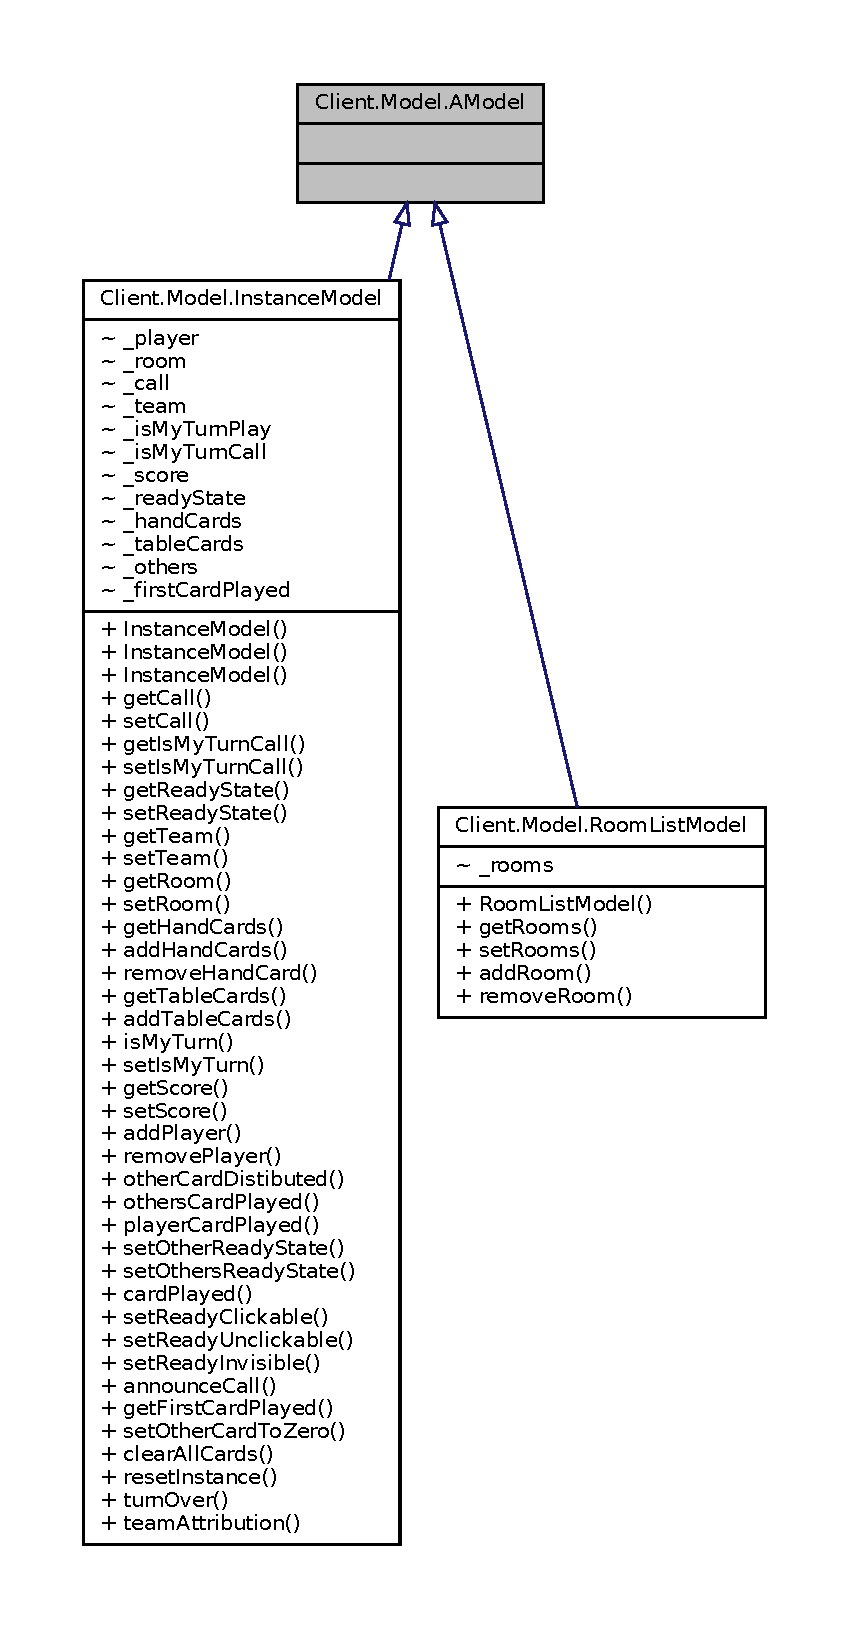
\includegraphics[height=550pt]{classClient_1_1Model_1_1AModel__inherit__graph}
\end{center}
\end{figure}


Collaboration diagram for Client.\+Model.\+A\+Model\+:
\nopagebreak
\begin{figure}[H]
\begin{center}
\leavevmode
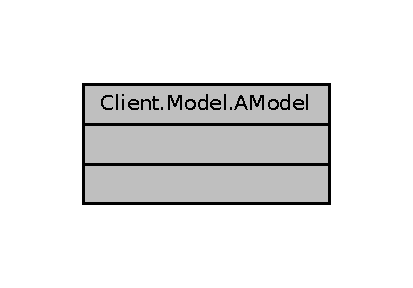
\includegraphics[width=198pt]{classClient_1_1Model_1_1AModel__coll__graph}
\end{center}
\end{figure}


The documentation for this class was generated from the following file\+:\begin{DoxyCompactItemize}
\item 
/home/tetard/\+Idea\+Projects/j\+Coinche/\+Java\+\_\+jcoinche\+\_\+2017/src/main/java/\+Client/\+Model/\mbox{\hyperlink{AModel_8java}{A\+Model.\+java}}\end{DoxyCompactItemize}

\hypertarget{classCommon_1_1AreYouReady}{}\section{Common.\+Are\+You\+Ready Class Reference}
\label{classCommon_1_1AreYouReady}\index{Common.\+Are\+You\+Ready@{Common.\+Are\+You\+Ready}}


Collaboration diagram for Common.\+Are\+You\+Ready\+:
\nopagebreak
\begin{figure}[H]
\begin{center}
\leavevmode
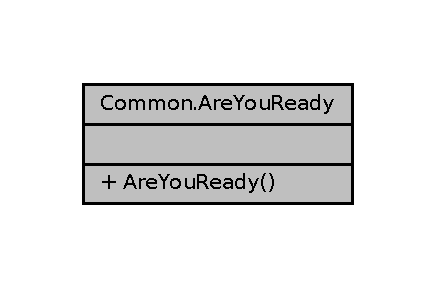
\includegraphics[width=209pt]{classCommon_1_1AreYouReady__coll__graph}
\end{center}
\end{figure}
\subsection*{Public Member Functions}
\begin{DoxyCompactItemize}
\item 
\mbox{\hyperlink{classCommon_1_1AreYouReady_a7c96896f70b28c0f70cec4f96fcaf64a}{Are\+You\+Ready}} ()
\end{DoxyCompactItemize}


\subsection{Constructor \& Destructor Documentation}
\mbox{\Hypertarget{classCommon_1_1AreYouReady_a7c96896f70b28c0f70cec4f96fcaf64a}\label{classCommon_1_1AreYouReady_a7c96896f70b28c0f70cec4f96fcaf64a}} 
\index{Common\+::\+Are\+You\+Ready@{Common\+::\+Are\+You\+Ready}!Are\+You\+Ready@{Are\+You\+Ready}}
\index{Are\+You\+Ready@{Are\+You\+Ready}!Common\+::\+Are\+You\+Ready@{Common\+::\+Are\+You\+Ready}}
\subsubsection{\texorpdfstring{Are\+You\+Ready()}{AreYouReady()}}
{\footnotesize\ttfamily Common.\+Are\+You\+Ready.\+Are\+You\+Ready (\begin{DoxyParamCaption}{ }\end{DoxyParamCaption})\hspace{0.3cm}{\ttfamily [inline]}}



The documentation for this class was generated from the following file\+:\begin{DoxyCompactItemize}
\item 
/home/tetard/\+Idea\+Projects/j\+Coinche/\+Java\+\_\+jcoinche\+\_\+2017/src/main/java/\+Common/\mbox{\hyperlink{AreYouReady_8java}{Are\+You\+Ready.\+java}}\end{DoxyCompactItemize}

\hypertarget{classCommon_1_1AskCreateRoom}{}\section{Common.\+Ask\+Create\+Room Class Reference}
\label{classCommon_1_1AskCreateRoom}\index{Common.\+Ask\+Create\+Room@{Common.\+Ask\+Create\+Room}}


Collaboration diagram for Common.\+Ask\+Create\+Room\+:
\nopagebreak
\begin{figure}[H]
\begin{center}
\leavevmode
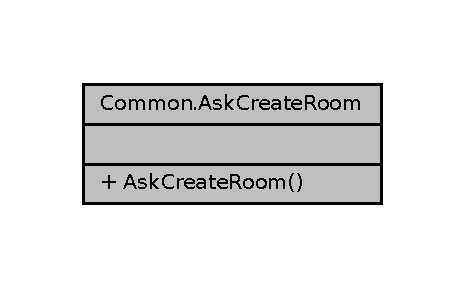
\includegraphics[width=223pt]{classCommon_1_1AskCreateRoom__coll__graph}
\end{center}
\end{figure}
\subsection*{Public Member Functions}
\begin{DoxyCompactItemize}
\item 
\mbox{\hyperlink{classCommon_1_1AskCreateRoom_ad7300cacf0663fd4f4a618219ae41ab3}{Ask\+Create\+Room}} ()
\end{DoxyCompactItemize}


\subsection{Constructor \& Destructor Documentation}
\mbox{\Hypertarget{classCommon_1_1AskCreateRoom_ad7300cacf0663fd4f4a618219ae41ab3}\label{classCommon_1_1AskCreateRoom_ad7300cacf0663fd4f4a618219ae41ab3}} 
\index{Common\+::\+Ask\+Create\+Room@{Common\+::\+Ask\+Create\+Room}!Ask\+Create\+Room@{Ask\+Create\+Room}}
\index{Ask\+Create\+Room@{Ask\+Create\+Room}!Common\+::\+Ask\+Create\+Room@{Common\+::\+Ask\+Create\+Room}}
\subsubsection{\texorpdfstring{Ask\+Create\+Room()}{AskCreateRoom()}}
{\footnotesize\ttfamily Common.\+Ask\+Create\+Room.\+Ask\+Create\+Room (\begin{DoxyParamCaption}{ }\end{DoxyParamCaption})\hspace{0.3cm}{\ttfamily [inline]}}



The documentation for this class was generated from the following file\+:\begin{DoxyCompactItemize}
\item 
/home/tetard/\+Idea\+Projects/j\+Coinche/\+Java\+\_\+jcoinche\+\_\+2017/src/main/java/\+Common/\mbox{\hyperlink{AskCreateRoom_8java}{Ask\+Create\+Room.\+java}}\end{DoxyCompactItemize}

\hypertarget{classCommon_1_1AskUserAuth}{}\section{Common.\+Ask\+User\+Auth Class Reference}
\label{classCommon_1_1AskUserAuth}\index{Common.\+Ask\+User\+Auth@{Common.\+Ask\+User\+Auth}}


Collaboration diagram for Common.\+Ask\+User\+Auth\+:
\nopagebreak
\begin{figure}[H]
\begin{center}
\leavevmode
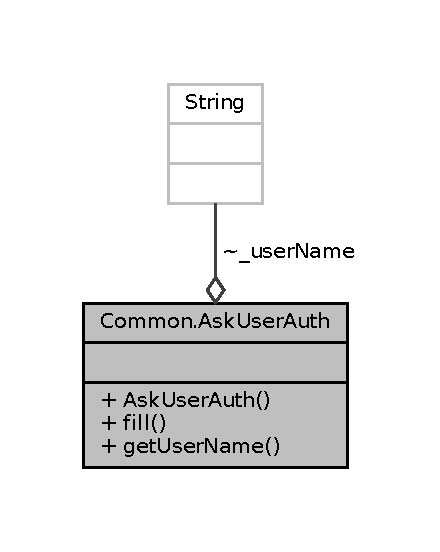
\includegraphics[width=211pt]{classCommon_1_1AskUserAuth__coll__graph}
\end{center}
\end{figure}
\subsection*{Public Member Functions}
\begin{DoxyCompactItemize}
\item 
\mbox{\hyperlink{classCommon_1_1AskUserAuth_afd1ec4231586d78ba3e42cda8416b120}{Ask\+User\+Auth}} ()
\item 
\mbox{\hyperlink{classCommon_1_1AskUserAuth}{Ask\+User\+Auth}} \mbox{\hyperlink{classCommon_1_1AskUserAuth_a1d4f4f3c59ac514089350064ef2d6aa8}{fill}} (String user\+Name)
\item 
String \mbox{\hyperlink{classCommon_1_1AskUserAuth_a123a0212f009ba34d8455a405cb90c0c}{get\+User\+Name}} ()
\end{DoxyCompactItemize}


\subsection{Constructor \& Destructor Documentation}
\mbox{\Hypertarget{classCommon_1_1AskUserAuth_afd1ec4231586d78ba3e42cda8416b120}\label{classCommon_1_1AskUserAuth_afd1ec4231586d78ba3e42cda8416b120}} 
\index{Common\+::\+Ask\+User\+Auth@{Common\+::\+Ask\+User\+Auth}!Ask\+User\+Auth@{Ask\+User\+Auth}}
\index{Ask\+User\+Auth@{Ask\+User\+Auth}!Common\+::\+Ask\+User\+Auth@{Common\+::\+Ask\+User\+Auth}}
\subsubsection{\texorpdfstring{Ask\+User\+Auth()}{AskUserAuth()}}
{\footnotesize\ttfamily Common.\+Ask\+User\+Auth.\+Ask\+User\+Auth (\begin{DoxyParamCaption}{ }\end{DoxyParamCaption})\hspace{0.3cm}{\ttfamily [inline]}}



\subsection{Member Function Documentation}
\mbox{\Hypertarget{classCommon_1_1AskUserAuth_a1d4f4f3c59ac514089350064ef2d6aa8}\label{classCommon_1_1AskUserAuth_a1d4f4f3c59ac514089350064ef2d6aa8}} 
\index{Common\+::\+Ask\+User\+Auth@{Common\+::\+Ask\+User\+Auth}!fill@{fill}}
\index{fill@{fill}!Common\+::\+Ask\+User\+Auth@{Common\+::\+Ask\+User\+Auth}}
\subsubsection{\texorpdfstring{fill()}{fill()}}
{\footnotesize\ttfamily \mbox{\hyperlink{classCommon_1_1AskUserAuth}{Ask\+User\+Auth}} Common.\+Ask\+User\+Auth.\+fill (\begin{DoxyParamCaption}\item[{String}]{user\+Name }\end{DoxyParamCaption})\hspace{0.3cm}{\ttfamily [inline]}}

\mbox{\Hypertarget{classCommon_1_1AskUserAuth_a123a0212f009ba34d8455a405cb90c0c}\label{classCommon_1_1AskUserAuth_a123a0212f009ba34d8455a405cb90c0c}} 
\index{Common\+::\+Ask\+User\+Auth@{Common\+::\+Ask\+User\+Auth}!get\+User\+Name@{get\+User\+Name}}
\index{get\+User\+Name@{get\+User\+Name}!Common\+::\+Ask\+User\+Auth@{Common\+::\+Ask\+User\+Auth}}
\subsubsection{\texorpdfstring{get\+User\+Name()}{getUserName()}}
{\footnotesize\ttfamily String Common.\+Ask\+User\+Auth.\+get\+User\+Name (\begin{DoxyParamCaption}{ }\end{DoxyParamCaption})\hspace{0.3cm}{\ttfamily [inline]}}



The documentation for this class was generated from the following file\+:\begin{DoxyCompactItemize}
\item 
/home/tetard/\+Idea\+Projects/j\+Coinche/\+Java\+\_\+jcoinche\+\_\+2017/src/main/java/\+Common/\mbox{\hyperlink{AskUserAuth_8java}{Ask\+User\+Auth.\+java}}\end{DoxyCompactItemize}

\hypertarget{classCommon_1_1AuthAnswer}{}\section{Common.\+Auth\+Answer Class Reference}
\label{classCommon_1_1AuthAnswer}\index{Common.\+Auth\+Answer@{Common.\+Auth\+Answer}}


Collaboration diagram for Common.\+Auth\+Answer\+:
\nopagebreak
\begin{figure}[H]
\begin{center}
\leavevmode
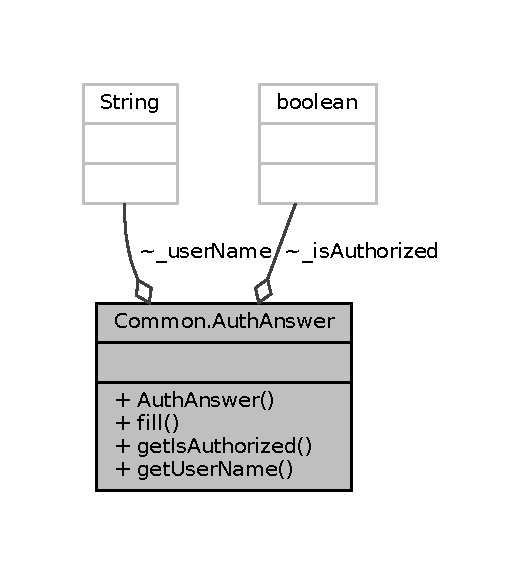
\includegraphics[width=252pt]{classCommon_1_1AuthAnswer__coll__graph}
\end{center}
\end{figure}
\subsection*{Public Member Functions}
\begin{DoxyCompactItemize}
\item 
\mbox{\hyperlink{classCommon_1_1AuthAnswer_ad50ba31140e0a04d1fa5e3fea5fd45bf}{Auth\+Answer}} ()
\item 
\mbox{\hyperlink{classCommon_1_1AuthAnswer}{Auth\+Answer}} \mbox{\hyperlink{classCommon_1_1AuthAnswer_a29e5a9ecc3b5d8e02c3ad157750c6594}{fill}} (boolean is\+Authorized, String user\+Name)
\item 
boolean \mbox{\hyperlink{classCommon_1_1AuthAnswer_a3e8d1c0d8a22f1674dbe041eaec8603d}{get\+Is\+Authorized}} ()
\item 
String \mbox{\hyperlink{classCommon_1_1AuthAnswer_aa175f09bf18de47d5a75cf88f675a56d}{get\+User\+Name}} ()
\end{DoxyCompactItemize}


\subsection{Constructor \& Destructor Documentation}
\mbox{\Hypertarget{classCommon_1_1AuthAnswer_ad50ba31140e0a04d1fa5e3fea5fd45bf}\label{classCommon_1_1AuthAnswer_ad50ba31140e0a04d1fa5e3fea5fd45bf}} 
\index{Common\+::\+Auth\+Answer@{Common\+::\+Auth\+Answer}!Auth\+Answer@{Auth\+Answer}}
\index{Auth\+Answer@{Auth\+Answer}!Common\+::\+Auth\+Answer@{Common\+::\+Auth\+Answer}}
\subsubsection{\texorpdfstring{Auth\+Answer()}{AuthAnswer()}}
{\footnotesize\ttfamily Common.\+Auth\+Answer.\+Auth\+Answer (\begin{DoxyParamCaption}{ }\end{DoxyParamCaption})\hspace{0.3cm}{\ttfamily [inline]}}



\subsection{Member Function Documentation}
\mbox{\Hypertarget{classCommon_1_1AuthAnswer_a29e5a9ecc3b5d8e02c3ad157750c6594}\label{classCommon_1_1AuthAnswer_a29e5a9ecc3b5d8e02c3ad157750c6594}} 
\index{Common\+::\+Auth\+Answer@{Common\+::\+Auth\+Answer}!fill@{fill}}
\index{fill@{fill}!Common\+::\+Auth\+Answer@{Common\+::\+Auth\+Answer}}
\subsubsection{\texorpdfstring{fill()}{fill()}}
{\footnotesize\ttfamily \mbox{\hyperlink{classCommon_1_1AuthAnswer}{Auth\+Answer}} Common.\+Auth\+Answer.\+fill (\begin{DoxyParamCaption}\item[{boolean}]{is\+Authorized,  }\item[{String}]{user\+Name }\end{DoxyParamCaption})\hspace{0.3cm}{\ttfamily [inline]}}

\mbox{\Hypertarget{classCommon_1_1AuthAnswer_a3e8d1c0d8a22f1674dbe041eaec8603d}\label{classCommon_1_1AuthAnswer_a3e8d1c0d8a22f1674dbe041eaec8603d}} 
\index{Common\+::\+Auth\+Answer@{Common\+::\+Auth\+Answer}!get\+Is\+Authorized@{get\+Is\+Authorized}}
\index{get\+Is\+Authorized@{get\+Is\+Authorized}!Common\+::\+Auth\+Answer@{Common\+::\+Auth\+Answer}}
\subsubsection{\texorpdfstring{get\+Is\+Authorized()}{getIsAuthorized()}}
{\footnotesize\ttfamily boolean Common.\+Auth\+Answer.\+get\+Is\+Authorized (\begin{DoxyParamCaption}{ }\end{DoxyParamCaption})\hspace{0.3cm}{\ttfamily [inline]}}

\mbox{\Hypertarget{classCommon_1_1AuthAnswer_aa175f09bf18de47d5a75cf88f675a56d}\label{classCommon_1_1AuthAnswer_aa175f09bf18de47d5a75cf88f675a56d}} 
\index{Common\+::\+Auth\+Answer@{Common\+::\+Auth\+Answer}!get\+User\+Name@{get\+User\+Name}}
\index{get\+User\+Name@{get\+User\+Name}!Common\+::\+Auth\+Answer@{Common\+::\+Auth\+Answer}}
\subsubsection{\texorpdfstring{get\+User\+Name()}{getUserName()}}
{\footnotesize\ttfamily String Common.\+Auth\+Answer.\+get\+User\+Name (\begin{DoxyParamCaption}{ }\end{DoxyParamCaption})\hspace{0.3cm}{\ttfamily [inline]}}



The documentation for this class was generated from the following file\+:\begin{DoxyCompactItemize}
\item 
/home/tetard/\+Idea\+Projects/j\+Coinche/\+Java\+\_\+jcoinche\+\_\+2017/src/main/java/\+Common/\mbox{\hyperlink{AuthAnswer_8java}{Auth\+Answer.\+java}}\end{DoxyCompactItemize}

\hypertarget{classClient_1_1BinaryTreeRules}{}\section{Client.\+Binary\+Tree\+Rules Class Reference}
\label{classClient_1_1BinaryTreeRules}\index{Client.\+Binary\+Tree\+Rules@{Client.\+Binary\+Tree\+Rules}}


Collaboration diagram for Client.\+Binary\+Tree\+Rules\+:
\nopagebreak
\begin{figure}[H]
\begin{center}
\leavevmode
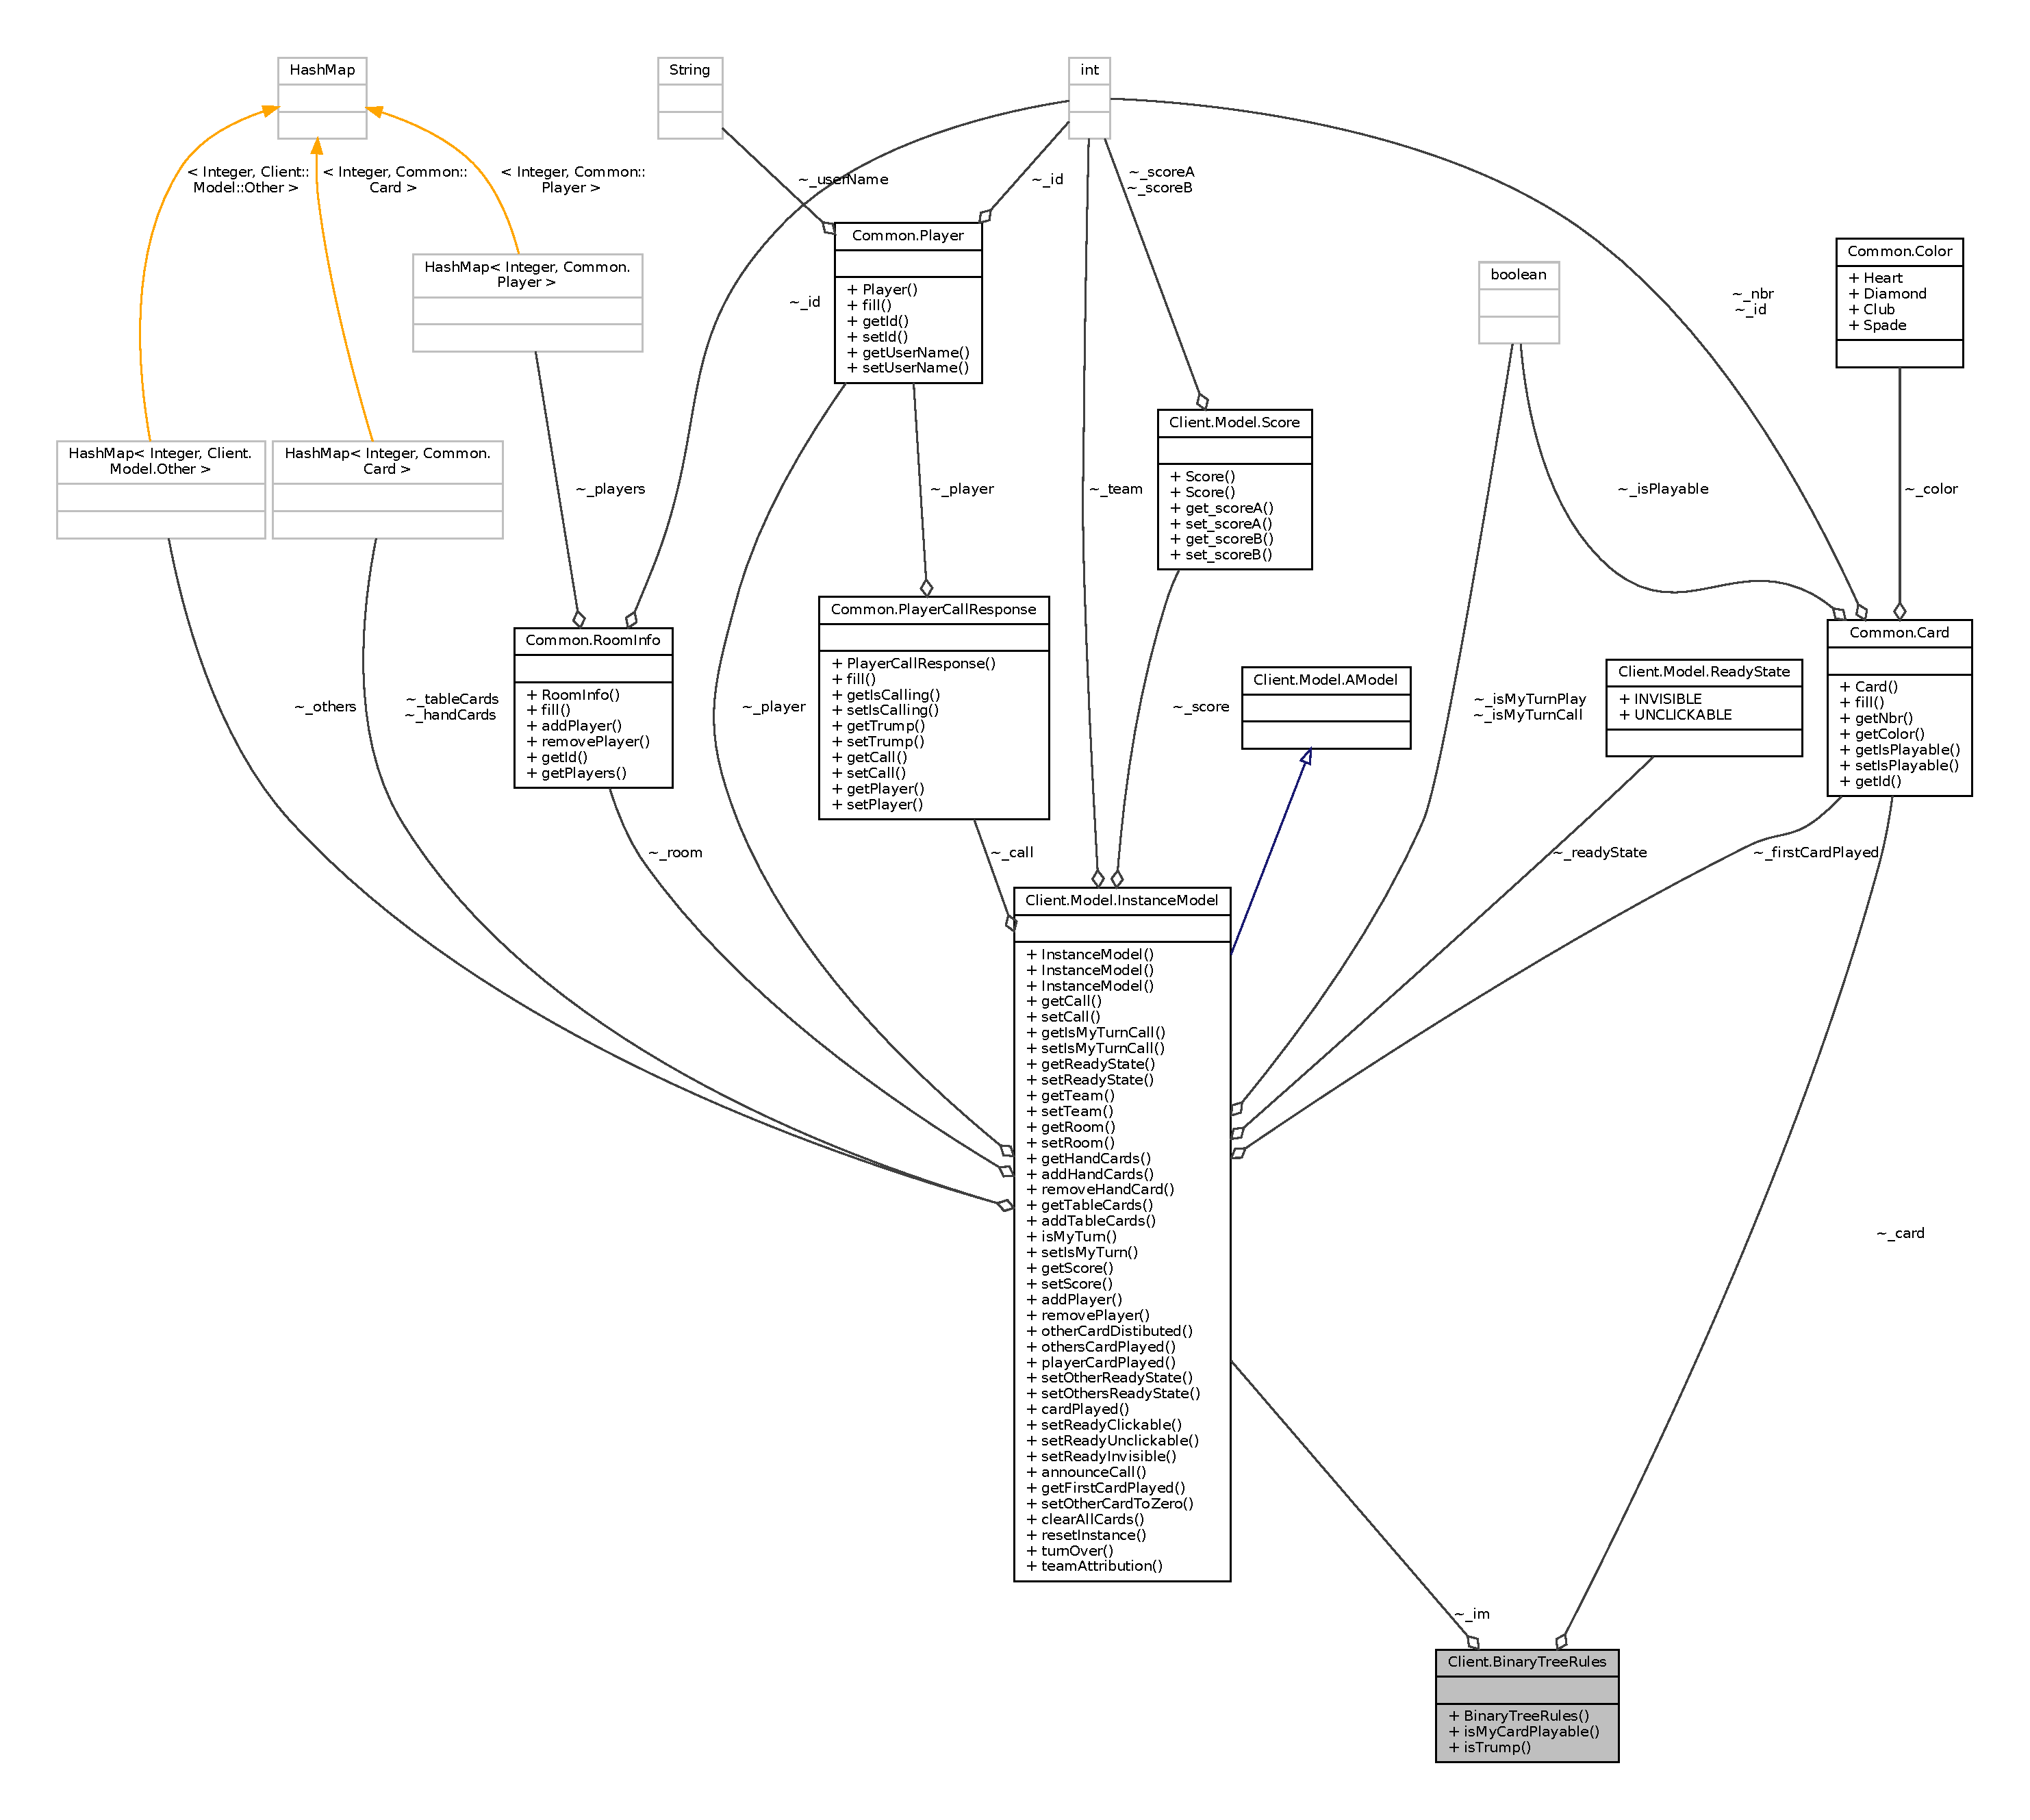
\includegraphics[width=350pt]{classClient_1_1BinaryTreeRules__coll__graph}
\end{center}
\end{figure}
\subsection*{Public Member Functions}
\begin{DoxyCompactItemize}
\item 
\mbox{\hyperlink{classClient_1_1BinaryTreeRules_ab6c1e397f8796077e1c7b4f0b830c2bc}{Binary\+Tree\+Rules}} ()
\item 
boolean \mbox{\hyperlink{classClient_1_1BinaryTreeRules_ae1e5dff7d60911140f0dace0b1d3e346}{is\+My\+Card\+Playable}} (\mbox{\hyperlink{classClient_1_1Model_1_1InstanceModel}{Instance\+Model}} im, \mbox{\hyperlink{classCommon_1_1Card}{Card}} card)
\item 
boolean \mbox{\hyperlink{classClient_1_1BinaryTreeRules_a27149c7f4a1039d0baf2d5f19f56b6ce}{is\+Trump}} (\mbox{\hyperlink{classCommon_1_1Card}{Card}} card)
\end{DoxyCompactItemize}


\subsection{Constructor \& Destructor Documentation}
\mbox{\Hypertarget{classClient_1_1BinaryTreeRules_ab6c1e397f8796077e1c7b4f0b830c2bc}\label{classClient_1_1BinaryTreeRules_ab6c1e397f8796077e1c7b4f0b830c2bc}} 
\index{Client\+::\+Binary\+Tree\+Rules@{Client\+::\+Binary\+Tree\+Rules}!Binary\+Tree\+Rules@{Binary\+Tree\+Rules}}
\index{Binary\+Tree\+Rules@{Binary\+Tree\+Rules}!Client\+::\+Binary\+Tree\+Rules@{Client\+::\+Binary\+Tree\+Rules}}
\subsubsection{\texorpdfstring{Binary\+Tree\+Rules()}{BinaryTreeRules()}}
{\footnotesize\ttfamily Client.\+Binary\+Tree\+Rules.\+Binary\+Tree\+Rules (\begin{DoxyParamCaption}{ }\end{DoxyParamCaption})\hspace{0.3cm}{\ttfamily [inline]}}



\subsection{Member Function Documentation}
\mbox{\Hypertarget{classClient_1_1BinaryTreeRules_ae1e5dff7d60911140f0dace0b1d3e346}\label{classClient_1_1BinaryTreeRules_ae1e5dff7d60911140f0dace0b1d3e346}} 
\index{Client\+::\+Binary\+Tree\+Rules@{Client\+::\+Binary\+Tree\+Rules}!is\+My\+Card\+Playable@{is\+My\+Card\+Playable}}
\index{is\+My\+Card\+Playable@{is\+My\+Card\+Playable}!Client\+::\+Binary\+Tree\+Rules@{Client\+::\+Binary\+Tree\+Rules}}
\subsubsection{\texorpdfstring{is\+My\+Card\+Playable()}{isMyCardPlayable()}}
{\footnotesize\ttfamily boolean Client.\+Binary\+Tree\+Rules.\+is\+My\+Card\+Playable (\begin{DoxyParamCaption}\item[{\mbox{\hyperlink{classClient_1_1Model_1_1InstanceModel}{Instance\+Model}}}]{im,  }\item[{\mbox{\hyperlink{classCommon_1_1Card}{Card}}}]{card }\end{DoxyParamCaption})\hspace{0.3cm}{\ttfamily [inline]}}

\mbox{\Hypertarget{classClient_1_1BinaryTreeRules_a27149c7f4a1039d0baf2d5f19f56b6ce}\label{classClient_1_1BinaryTreeRules_a27149c7f4a1039d0baf2d5f19f56b6ce}} 
\index{Client\+::\+Binary\+Tree\+Rules@{Client\+::\+Binary\+Tree\+Rules}!is\+Trump@{is\+Trump}}
\index{is\+Trump@{is\+Trump}!Client\+::\+Binary\+Tree\+Rules@{Client\+::\+Binary\+Tree\+Rules}}
\subsubsection{\texorpdfstring{is\+Trump()}{isTrump()}}
{\footnotesize\ttfamily boolean Client.\+Binary\+Tree\+Rules.\+is\+Trump (\begin{DoxyParamCaption}\item[{\mbox{\hyperlink{classCommon_1_1Card}{Card}}}]{card }\end{DoxyParamCaption})\hspace{0.3cm}{\ttfamily [inline]}}



The documentation for this class was generated from the following file\+:\begin{DoxyCompactItemize}
\item 
/home/tetard/\+Idea\+Projects/j\+Coinche/\+Java\+\_\+jcoinche\+\_\+2017/src/main/java/\+Client/\mbox{\hyperlink{BinaryTreeRules_8java}{Binary\+Tree\+Rules.\+java}}\end{DoxyCompactItemize}

\hypertarget{classCommon_1_1Card}{}\section{Common.\+Card Class Reference}
\label{classCommon_1_1Card}\index{Common.\+Card@{Common.\+Card}}


Collaboration diagram for Common.\+Card\+:
\nopagebreak
\begin{figure}[H]
\begin{center}
\leavevmode
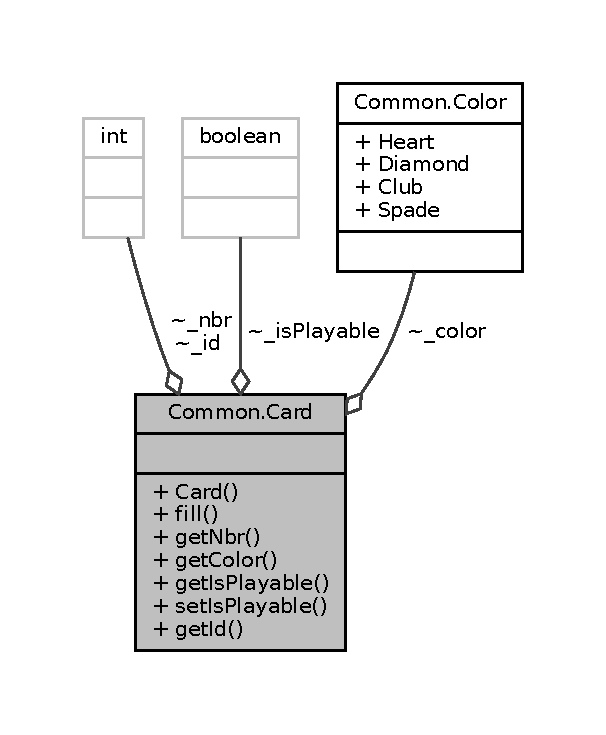
\includegraphics[width=291pt]{classCommon_1_1Card__coll__graph}
\end{center}
\end{figure}
\subsection*{Public Member Functions}
\begin{DoxyCompactItemize}
\item 
\mbox{\hyperlink{classCommon_1_1Card_aa34725a77b9b1303b5c67b9c2a9cf957}{Card}} ()
\item 
\mbox{\hyperlink{classCommon_1_1Card}{Card}} \mbox{\hyperlink{classCommon_1_1Card_a98fe165a8fb52b177efb8cf58961d876}{fill}} (int id, int nbr, \mbox{\hyperlink{enumCommon_1_1Color}{Color}} color)
\item 
int \mbox{\hyperlink{classCommon_1_1Card_a0d64a4a92a9e32d68465b77d646a4914}{get\+Nbr}} ()
\item 
\mbox{\hyperlink{enumCommon_1_1Color}{Color}} \mbox{\hyperlink{classCommon_1_1Card_a7527a91352a5c110c79a175f719b3abc}{get\+Color}} ()
\item 
boolean \mbox{\hyperlink{classCommon_1_1Card_a431524be99d59498172ca9d49b378623}{get\+Is\+Playable}} ()
\item 
void \mbox{\hyperlink{classCommon_1_1Card_a662df61afb520d172fb59c2c8d172386}{set\+Is\+Playable}} (boolean is\+Playable)
\item 
int \mbox{\hyperlink{classCommon_1_1Card_a4dcabbdd3a17d9c898cdd3832fd68c9e}{get\+Id}} ()
\end{DoxyCompactItemize}


\subsection{Constructor \& Destructor Documentation}
\mbox{\Hypertarget{classCommon_1_1Card_aa34725a77b9b1303b5c67b9c2a9cf957}\label{classCommon_1_1Card_aa34725a77b9b1303b5c67b9c2a9cf957}} 
\index{Common\+::\+Card@{Common\+::\+Card}!Card@{Card}}
\index{Card@{Card}!Common\+::\+Card@{Common\+::\+Card}}
\subsubsection{\texorpdfstring{Card()}{Card()}}
{\footnotesize\ttfamily Common.\+Card.\+Card (\begin{DoxyParamCaption}{ }\end{DoxyParamCaption})\hspace{0.3cm}{\ttfamily [inline]}}



\subsection{Member Function Documentation}
\mbox{\Hypertarget{classCommon_1_1Card_a98fe165a8fb52b177efb8cf58961d876}\label{classCommon_1_1Card_a98fe165a8fb52b177efb8cf58961d876}} 
\index{Common\+::\+Card@{Common\+::\+Card}!fill@{fill}}
\index{fill@{fill}!Common\+::\+Card@{Common\+::\+Card}}
\subsubsection{\texorpdfstring{fill()}{fill()}}
{\footnotesize\ttfamily \mbox{\hyperlink{classCommon_1_1Card}{Card}} Common.\+Card.\+fill (\begin{DoxyParamCaption}\item[{int}]{id,  }\item[{int}]{nbr,  }\item[{\mbox{\hyperlink{enumCommon_1_1Color}{Color}}}]{color }\end{DoxyParamCaption})\hspace{0.3cm}{\ttfamily [inline]}}

\mbox{\Hypertarget{classCommon_1_1Card_a7527a91352a5c110c79a175f719b3abc}\label{classCommon_1_1Card_a7527a91352a5c110c79a175f719b3abc}} 
\index{Common\+::\+Card@{Common\+::\+Card}!get\+Color@{get\+Color}}
\index{get\+Color@{get\+Color}!Common\+::\+Card@{Common\+::\+Card}}
\subsubsection{\texorpdfstring{get\+Color()}{getColor()}}
{\footnotesize\ttfamily \mbox{\hyperlink{enumCommon_1_1Color}{Color}} Common.\+Card.\+get\+Color (\begin{DoxyParamCaption}{ }\end{DoxyParamCaption})\hspace{0.3cm}{\ttfamily [inline]}}

\mbox{\Hypertarget{classCommon_1_1Card_a4dcabbdd3a17d9c898cdd3832fd68c9e}\label{classCommon_1_1Card_a4dcabbdd3a17d9c898cdd3832fd68c9e}} 
\index{Common\+::\+Card@{Common\+::\+Card}!get\+Id@{get\+Id}}
\index{get\+Id@{get\+Id}!Common\+::\+Card@{Common\+::\+Card}}
\subsubsection{\texorpdfstring{get\+Id()}{getId()}}
{\footnotesize\ttfamily int Common.\+Card.\+get\+Id (\begin{DoxyParamCaption}{ }\end{DoxyParamCaption})\hspace{0.3cm}{\ttfamily [inline]}}

\mbox{\Hypertarget{classCommon_1_1Card_a431524be99d59498172ca9d49b378623}\label{classCommon_1_1Card_a431524be99d59498172ca9d49b378623}} 
\index{Common\+::\+Card@{Common\+::\+Card}!get\+Is\+Playable@{get\+Is\+Playable}}
\index{get\+Is\+Playable@{get\+Is\+Playable}!Common\+::\+Card@{Common\+::\+Card}}
\subsubsection{\texorpdfstring{get\+Is\+Playable()}{getIsPlayable()}}
{\footnotesize\ttfamily boolean Common.\+Card.\+get\+Is\+Playable (\begin{DoxyParamCaption}{ }\end{DoxyParamCaption})\hspace{0.3cm}{\ttfamily [inline]}}

\mbox{\Hypertarget{classCommon_1_1Card_a0d64a4a92a9e32d68465b77d646a4914}\label{classCommon_1_1Card_a0d64a4a92a9e32d68465b77d646a4914}} 
\index{Common\+::\+Card@{Common\+::\+Card}!get\+Nbr@{get\+Nbr}}
\index{get\+Nbr@{get\+Nbr}!Common\+::\+Card@{Common\+::\+Card}}
\subsubsection{\texorpdfstring{get\+Nbr()}{getNbr()}}
{\footnotesize\ttfamily int Common.\+Card.\+get\+Nbr (\begin{DoxyParamCaption}{ }\end{DoxyParamCaption})\hspace{0.3cm}{\ttfamily [inline]}}

\mbox{\Hypertarget{classCommon_1_1Card_a662df61afb520d172fb59c2c8d172386}\label{classCommon_1_1Card_a662df61afb520d172fb59c2c8d172386}} 
\index{Common\+::\+Card@{Common\+::\+Card}!set\+Is\+Playable@{set\+Is\+Playable}}
\index{set\+Is\+Playable@{set\+Is\+Playable}!Common\+::\+Card@{Common\+::\+Card}}
\subsubsection{\texorpdfstring{set\+Is\+Playable()}{setIsPlayable()}}
{\footnotesize\ttfamily void Common.\+Card.\+set\+Is\+Playable (\begin{DoxyParamCaption}\item[{boolean}]{is\+Playable }\end{DoxyParamCaption})\hspace{0.3cm}{\ttfamily [inline]}}



The documentation for this class was generated from the following file\+:\begin{DoxyCompactItemize}
\item 
/home/tetard/\+Idea\+Projects/j\+Coinche/\+Java\+\_\+jcoinche\+\_\+2017/src/main/java/\+Common/\mbox{\hyperlink{Card_8java}{Card.\+java}}\end{DoxyCompactItemize}

\hypertarget{classCommon_1_1CardDistributed}{}\section{Common.\+Card\+Distributed Class Reference}
\label{classCommon_1_1CardDistributed}\index{Common.\+Card\+Distributed@{Common.\+Card\+Distributed}}


Collaboration diagram for Common.\+Card\+Distributed\+:
\nopagebreak
\begin{figure}[H]
\begin{center}
\leavevmode
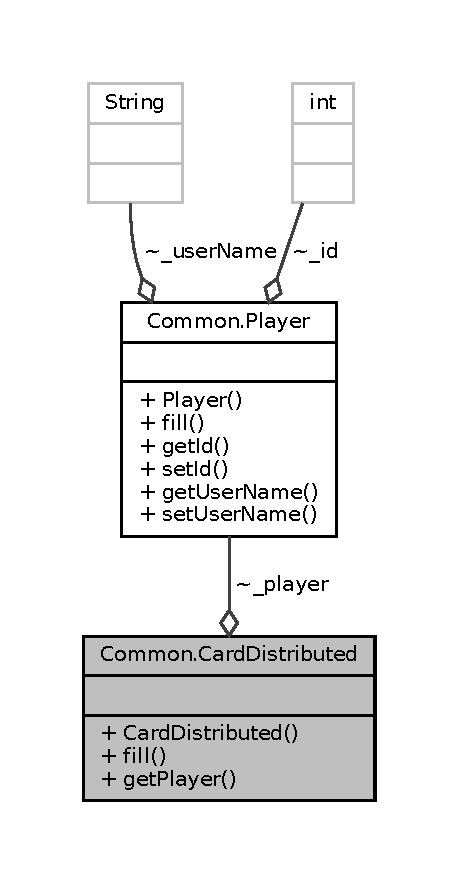
\includegraphics[width=220pt]{classCommon_1_1CardDistributed__coll__graph}
\end{center}
\end{figure}
\subsection*{Public Member Functions}
\begin{DoxyCompactItemize}
\item 
\mbox{\hyperlink{classCommon_1_1CardDistributed_a9e26a96371b98282d4428db7d020b1be}{Card\+Distributed}} ()
\item 
\mbox{\hyperlink{classCommon_1_1CardDistributed}{Card\+Distributed}} \mbox{\hyperlink{classCommon_1_1CardDistributed_af60eec7a32c061fc4bb88a8a48b78d96}{fill}} (\mbox{\hyperlink{classCommon_1_1Player}{Player}} player)
\item 
\mbox{\hyperlink{classCommon_1_1Player}{Player}} \mbox{\hyperlink{classCommon_1_1CardDistributed_a8640cb70a1303199c816d9271b5a1f7d}{get\+Player}} ()
\end{DoxyCompactItemize}


\subsection{Constructor \& Destructor Documentation}
\mbox{\Hypertarget{classCommon_1_1CardDistributed_a9e26a96371b98282d4428db7d020b1be}\label{classCommon_1_1CardDistributed_a9e26a96371b98282d4428db7d020b1be}} 
\index{Common\+::\+Card\+Distributed@{Common\+::\+Card\+Distributed}!Card\+Distributed@{Card\+Distributed}}
\index{Card\+Distributed@{Card\+Distributed}!Common\+::\+Card\+Distributed@{Common\+::\+Card\+Distributed}}
\subsubsection{\texorpdfstring{Card\+Distributed()}{CardDistributed()}}
{\footnotesize\ttfamily Common.\+Card\+Distributed.\+Card\+Distributed (\begin{DoxyParamCaption}{ }\end{DoxyParamCaption})\hspace{0.3cm}{\ttfamily [inline]}}



\subsection{Member Function Documentation}
\mbox{\Hypertarget{classCommon_1_1CardDistributed_af60eec7a32c061fc4bb88a8a48b78d96}\label{classCommon_1_1CardDistributed_af60eec7a32c061fc4bb88a8a48b78d96}} 
\index{Common\+::\+Card\+Distributed@{Common\+::\+Card\+Distributed}!fill@{fill}}
\index{fill@{fill}!Common\+::\+Card\+Distributed@{Common\+::\+Card\+Distributed}}
\subsubsection{\texorpdfstring{fill()}{fill()}}
{\footnotesize\ttfamily \mbox{\hyperlink{classCommon_1_1CardDistributed}{Card\+Distributed}} Common.\+Card\+Distributed.\+fill (\begin{DoxyParamCaption}\item[{\mbox{\hyperlink{classCommon_1_1Player}{Player}}}]{player }\end{DoxyParamCaption})\hspace{0.3cm}{\ttfamily [inline]}}

\mbox{\Hypertarget{classCommon_1_1CardDistributed_a8640cb70a1303199c816d9271b5a1f7d}\label{classCommon_1_1CardDistributed_a8640cb70a1303199c816d9271b5a1f7d}} 
\index{Common\+::\+Card\+Distributed@{Common\+::\+Card\+Distributed}!get\+Player@{get\+Player}}
\index{get\+Player@{get\+Player}!Common\+::\+Card\+Distributed@{Common\+::\+Card\+Distributed}}
\subsubsection{\texorpdfstring{get\+Player()}{getPlayer()}}
{\footnotesize\ttfamily \mbox{\hyperlink{classCommon_1_1Player}{Player}} Common.\+Card\+Distributed.\+get\+Player (\begin{DoxyParamCaption}{ }\end{DoxyParamCaption})\hspace{0.3cm}{\ttfamily [inline]}}



The documentation for this class was generated from the following file\+:\begin{DoxyCompactItemize}
\item 
/home/tetard/\+Idea\+Projects/j\+Coinche/\+Java\+\_\+jcoinche\+\_\+2017/src/main/java/\+Common/\mbox{\hyperlink{CardDistributed_8java}{Card\+Distributed.\+java}}\end{DoxyCompactItemize}

\hypertarget{classCommon_1_1CardPlayed}{}\section{Common.\+Card\+Played Class Reference}
\label{classCommon_1_1CardPlayed}\index{Common.\+Card\+Played@{Common.\+Card\+Played}}


Collaboration diagram for Common.\+Card\+Played\+:
\nopagebreak
\begin{figure}[H]
\begin{center}
\leavevmode
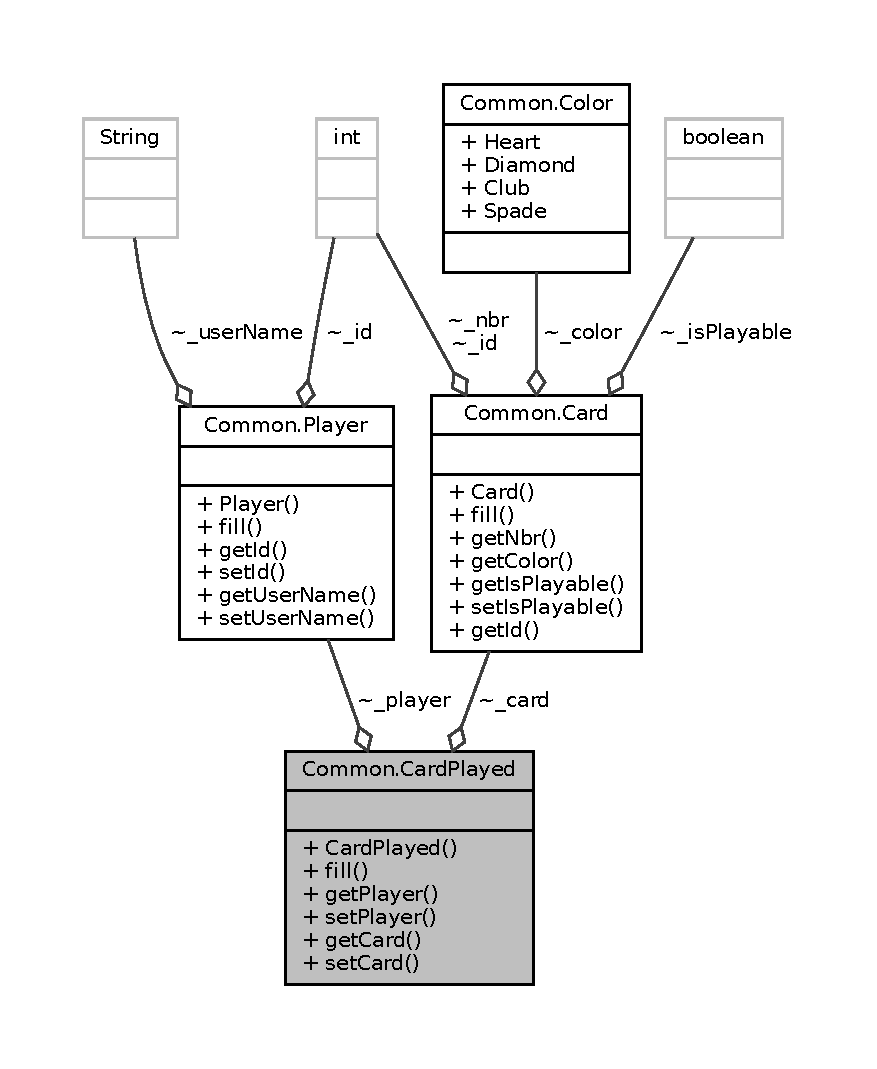
\includegraphics[width=350pt]{classCommon_1_1CardPlayed__coll__graph}
\end{center}
\end{figure}
\subsection*{Public Member Functions}
\begin{DoxyCompactItemize}
\item 
\mbox{\hyperlink{classCommon_1_1CardPlayed_ac419f1ab40063fda2fd341bbc573881b}{Card\+Played}} ()
\item 
void \mbox{\hyperlink{classCommon_1_1CardPlayed_a1fd0f482239ffca7af9f38e612e968ec}{fill}} (\mbox{\hyperlink{classCommon_1_1Player}{Player}} player, \mbox{\hyperlink{classCommon_1_1Card}{Card}} card)
\item 
\mbox{\hyperlink{classCommon_1_1Player}{Player}} \mbox{\hyperlink{classCommon_1_1CardPlayed_a2d9995ec0df85ae12c7dc77776f8043e}{get\+Player}} ()
\item 
void \mbox{\hyperlink{classCommon_1_1CardPlayed_ab1e8317983a794c99aef643569ba93ce}{set\+Player}} (\mbox{\hyperlink{classCommon_1_1Player}{Player}} player)
\item 
\mbox{\hyperlink{classCommon_1_1Card}{Card}} \mbox{\hyperlink{classCommon_1_1CardPlayed_a5db9f3b0525f633cf74ca94b379c80ff}{get\+Card}} ()
\item 
void \mbox{\hyperlink{classCommon_1_1CardPlayed_ad456e1fb513fb05d53f21d80f399fa24}{set\+Card}} (\mbox{\hyperlink{classCommon_1_1Card}{Card}} card)
\end{DoxyCompactItemize}


\subsection{Constructor \& Destructor Documentation}
\mbox{\Hypertarget{classCommon_1_1CardPlayed_ac419f1ab40063fda2fd341bbc573881b}\label{classCommon_1_1CardPlayed_ac419f1ab40063fda2fd341bbc573881b}} 
\index{Common\+::\+Card\+Played@{Common\+::\+Card\+Played}!Card\+Played@{Card\+Played}}
\index{Card\+Played@{Card\+Played}!Common\+::\+Card\+Played@{Common\+::\+Card\+Played}}
\subsubsection{\texorpdfstring{Card\+Played()}{CardPlayed()}}
{\footnotesize\ttfamily Common.\+Card\+Played.\+Card\+Played (\begin{DoxyParamCaption}{ }\end{DoxyParamCaption})\hspace{0.3cm}{\ttfamily [inline]}}



\subsection{Member Function Documentation}
\mbox{\Hypertarget{classCommon_1_1CardPlayed_a1fd0f482239ffca7af9f38e612e968ec}\label{classCommon_1_1CardPlayed_a1fd0f482239ffca7af9f38e612e968ec}} 
\index{Common\+::\+Card\+Played@{Common\+::\+Card\+Played}!fill@{fill}}
\index{fill@{fill}!Common\+::\+Card\+Played@{Common\+::\+Card\+Played}}
\subsubsection{\texorpdfstring{fill()}{fill()}}
{\footnotesize\ttfamily void Common.\+Card\+Played.\+fill (\begin{DoxyParamCaption}\item[{\mbox{\hyperlink{classCommon_1_1Player}{Player}}}]{player,  }\item[{\mbox{\hyperlink{classCommon_1_1Card}{Card}}}]{card }\end{DoxyParamCaption})\hspace{0.3cm}{\ttfamily [inline]}}

\mbox{\Hypertarget{classCommon_1_1CardPlayed_a5db9f3b0525f633cf74ca94b379c80ff}\label{classCommon_1_1CardPlayed_a5db9f3b0525f633cf74ca94b379c80ff}} 
\index{Common\+::\+Card\+Played@{Common\+::\+Card\+Played}!get\+Card@{get\+Card}}
\index{get\+Card@{get\+Card}!Common\+::\+Card\+Played@{Common\+::\+Card\+Played}}
\subsubsection{\texorpdfstring{get\+Card()}{getCard()}}
{\footnotesize\ttfamily \mbox{\hyperlink{classCommon_1_1Card}{Card}} Common.\+Card\+Played.\+get\+Card (\begin{DoxyParamCaption}{ }\end{DoxyParamCaption})\hspace{0.3cm}{\ttfamily [inline]}}

\mbox{\Hypertarget{classCommon_1_1CardPlayed_a2d9995ec0df85ae12c7dc77776f8043e}\label{classCommon_1_1CardPlayed_a2d9995ec0df85ae12c7dc77776f8043e}} 
\index{Common\+::\+Card\+Played@{Common\+::\+Card\+Played}!get\+Player@{get\+Player}}
\index{get\+Player@{get\+Player}!Common\+::\+Card\+Played@{Common\+::\+Card\+Played}}
\subsubsection{\texorpdfstring{get\+Player()}{getPlayer()}}
{\footnotesize\ttfamily \mbox{\hyperlink{classCommon_1_1Player}{Player}} Common.\+Card\+Played.\+get\+Player (\begin{DoxyParamCaption}{ }\end{DoxyParamCaption})\hspace{0.3cm}{\ttfamily [inline]}}

\mbox{\Hypertarget{classCommon_1_1CardPlayed_ad456e1fb513fb05d53f21d80f399fa24}\label{classCommon_1_1CardPlayed_ad456e1fb513fb05d53f21d80f399fa24}} 
\index{Common\+::\+Card\+Played@{Common\+::\+Card\+Played}!set\+Card@{set\+Card}}
\index{set\+Card@{set\+Card}!Common\+::\+Card\+Played@{Common\+::\+Card\+Played}}
\subsubsection{\texorpdfstring{set\+Card()}{setCard()}}
{\footnotesize\ttfamily void Common.\+Card\+Played.\+set\+Card (\begin{DoxyParamCaption}\item[{\mbox{\hyperlink{classCommon_1_1Card}{Card}}}]{card }\end{DoxyParamCaption})\hspace{0.3cm}{\ttfamily [inline]}}

\mbox{\Hypertarget{classCommon_1_1CardPlayed_ab1e8317983a794c99aef643569ba93ce}\label{classCommon_1_1CardPlayed_ab1e8317983a794c99aef643569ba93ce}} 
\index{Common\+::\+Card\+Played@{Common\+::\+Card\+Played}!set\+Player@{set\+Player}}
\index{set\+Player@{set\+Player}!Common\+::\+Card\+Played@{Common\+::\+Card\+Played}}
\subsubsection{\texorpdfstring{set\+Player()}{setPlayer()}}
{\footnotesize\ttfamily void Common.\+Card\+Played.\+set\+Player (\begin{DoxyParamCaption}\item[{\mbox{\hyperlink{classCommon_1_1Player}{Player}}}]{player }\end{DoxyParamCaption})\hspace{0.3cm}{\ttfamily [inline]}}



The documentation for this class was generated from the following file\+:\begin{DoxyCompactItemize}
\item 
/home/tetard/\+Idea\+Projects/j\+Coinche/\+Java\+\_\+jcoinche\+\_\+2017/src/main/java/\+Common/\mbox{\hyperlink{CardPlayed_8java}{Card\+Played.\+java}}\end{DoxyCompactItemize}

\hypertarget{classClient_1_1Model_1_1CardPrintable}{}\section{Client.\+Model.\+Card\+Printable Class Reference}
\label{classClient_1_1Model_1_1CardPrintable}\index{Client.\+Model.\+Card\+Printable@{Client.\+Model.\+Card\+Printable}}


Collaboration diagram for Client.\+Model.\+Card\+Printable\+:
\nopagebreak
\begin{figure}[H]
\begin{center}
\leavevmode
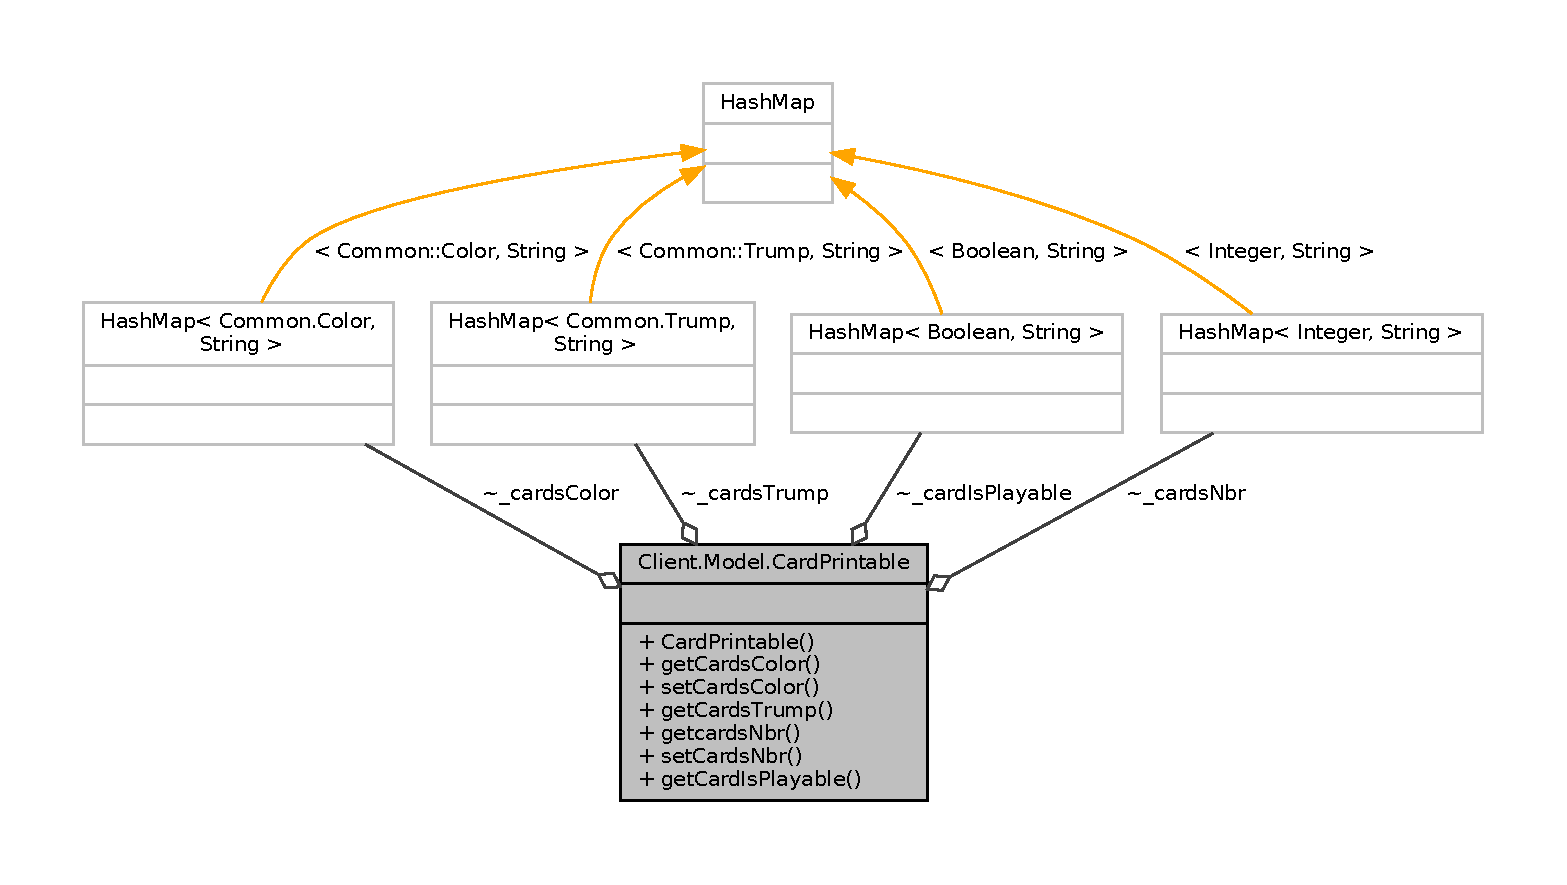
\includegraphics[width=350pt]{classClient_1_1Model_1_1CardPrintable__coll__graph}
\end{center}
\end{figure}
\subsection*{Public Member Functions}
\begin{DoxyCompactItemize}
\item 
\mbox{\hyperlink{classClient_1_1Model_1_1CardPrintable_a0d5529a8f38150b8247987de25e211f1}{Card\+Printable}} ()
\item 
Hash\+Map$<$ \mbox{\hyperlink{enumCommon_1_1Color}{Color}}, String $>$ \mbox{\hyperlink{classClient_1_1Model_1_1CardPrintable_a4e25b9c9e2f896c38226b90f6d70c3e1}{get\+Cards\+Color}} ()
\item 
void \mbox{\hyperlink{classClient_1_1Model_1_1CardPrintable_a274cad3b9d126733b8836925bf78fdcc}{set\+Cards\+Color}} (Hash\+Map$<$ \mbox{\hyperlink{enumCommon_1_1Color}{Color}}, String $>$ cards\+Color)
\item 
Hash\+Map$<$ \mbox{\hyperlink{enumCommon_1_1Trump}{Trump}}, String $>$ \mbox{\hyperlink{classClient_1_1Model_1_1CardPrintable_a2ea1954ac7f7d1e7d5722ca9ec3e47ec}{get\+Cards\+Trump}} ()
\item 
Hash\+Map$<$ Integer, String $>$ \mbox{\hyperlink{classClient_1_1Model_1_1CardPrintable_a822c686854b07df2db3081343f72ea72}{getcards\+Nbr}} ()
\item 
void \mbox{\hyperlink{classClient_1_1Model_1_1CardPrintable_a6a0d91fd25888e5db9c9ad82ea924c76}{set\+Cards\+Nbr}} (Hash\+Map cards)
\item 
Hash\+Map$<$ Boolean, String $>$ \mbox{\hyperlink{classClient_1_1Model_1_1CardPrintable_a632c8e7ba57e3ad447add89a99ee78f7}{get\+Card\+Is\+Playable}} ()
\end{DoxyCompactItemize}


\subsection{Constructor \& Destructor Documentation}
\mbox{\Hypertarget{classClient_1_1Model_1_1CardPrintable_a0d5529a8f38150b8247987de25e211f1}\label{classClient_1_1Model_1_1CardPrintable_a0d5529a8f38150b8247987de25e211f1}} 
\index{Client\+::\+Model\+::\+Card\+Printable@{Client\+::\+Model\+::\+Card\+Printable}!Card\+Printable@{Card\+Printable}}
\index{Card\+Printable@{Card\+Printable}!Client\+::\+Model\+::\+Card\+Printable@{Client\+::\+Model\+::\+Card\+Printable}}
\subsubsection{\texorpdfstring{Card\+Printable()}{CardPrintable()}}
{\footnotesize\ttfamily Client.\+Model.\+Card\+Printable.\+Card\+Printable (\begin{DoxyParamCaption}{ }\end{DoxyParamCaption})\hspace{0.3cm}{\ttfamily [inline]}}



\subsection{Member Function Documentation}
\mbox{\Hypertarget{classClient_1_1Model_1_1CardPrintable_a632c8e7ba57e3ad447add89a99ee78f7}\label{classClient_1_1Model_1_1CardPrintable_a632c8e7ba57e3ad447add89a99ee78f7}} 
\index{Client\+::\+Model\+::\+Card\+Printable@{Client\+::\+Model\+::\+Card\+Printable}!get\+Card\+Is\+Playable@{get\+Card\+Is\+Playable}}
\index{get\+Card\+Is\+Playable@{get\+Card\+Is\+Playable}!Client\+::\+Model\+::\+Card\+Printable@{Client\+::\+Model\+::\+Card\+Printable}}
\subsubsection{\texorpdfstring{get\+Card\+Is\+Playable()}{getCardIsPlayable()}}
{\footnotesize\ttfamily Hash\+Map$<$Boolean, String$>$ Client.\+Model.\+Card\+Printable.\+get\+Card\+Is\+Playable (\begin{DoxyParamCaption}{ }\end{DoxyParamCaption})\hspace{0.3cm}{\ttfamily [inline]}}

\mbox{\Hypertarget{classClient_1_1Model_1_1CardPrintable_a4e25b9c9e2f896c38226b90f6d70c3e1}\label{classClient_1_1Model_1_1CardPrintable_a4e25b9c9e2f896c38226b90f6d70c3e1}} 
\index{Client\+::\+Model\+::\+Card\+Printable@{Client\+::\+Model\+::\+Card\+Printable}!get\+Cards\+Color@{get\+Cards\+Color}}
\index{get\+Cards\+Color@{get\+Cards\+Color}!Client\+::\+Model\+::\+Card\+Printable@{Client\+::\+Model\+::\+Card\+Printable}}
\subsubsection{\texorpdfstring{get\+Cards\+Color()}{getCardsColor()}}
{\footnotesize\ttfamily Hash\+Map$<$\mbox{\hyperlink{enumCommon_1_1Color}{Color}}, String$>$ Client.\+Model.\+Card\+Printable.\+get\+Cards\+Color (\begin{DoxyParamCaption}{ }\end{DoxyParamCaption})\hspace{0.3cm}{\ttfamily [inline]}}

\mbox{\Hypertarget{classClient_1_1Model_1_1CardPrintable_a822c686854b07df2db3081343f72ea72}\label{classClient_1_1Model_1_1CardPrintable_a822c686854b07df2db3081343f72ea72}} 
\index{Client\+::\+Model\+::\+Card\+Printable@{Client\+::\+Model\+::\+Card\+Printable}!getcards\+Nbr@{getcards\+Nbr}}
\index{getcards\+Nbr@{getcards\+Nbr}!Client\+::\+Model\+::\+Card\+Printable@{Client\+::\+Model\+::\+Card\+Printable}}
\subsubsection{\texorpdfstring{getcards\+Nbr()}{getcardsNbr()}}
{\footnotesize\ttfamily Hash\+Map$<$Integer, String$>$ Client.\+Model.\+Card\+Printable.\+getcards\+Nbr (\begin{DoxyParamCaption}{ }\end{DoxyParamCaption})\hspace{0.3cm}{\ttfamily [inline]}}

\mbox{\Hypertarget{classClient_1_1Model_1_1CardPrintable_a2ea1954ac7f7d1e7d5722ca9ec3e47ec}\label{classClient_1_1Model_1_1CardPrintable_a2ea1954ac7f7d1e7d5722ca9ec3e47ec}} 
\index{Client\+::\+Model\+::\+Card\+Printable@{Client\+::\+Model\+::\+Card\+Printable}!get\+Cards\+Trump@{get\+Cards\+Trump}}
\index{get\+Cards\+Trump@{get\+Cards\+Trump}!Client\+::\+Model\+::\+Card\+Printable@{Client\+::\+Model\+::\+Card\+Printable}}
\subsubsection{\texorpdfstring{get\+Cards\+Trump()}{getCardsTrump()}}
{\footnotesize\ttfamily Hash\+Map$<$\mbox{\hyperlink{enumCommon_1_1Trump}{Trump}}, String$>$ Client.\+Model.\+Card\+Printable.\+get\+Cards\+Trump (\begin{DoxyParamCaption}{ }\end{DoxyParamCaption})\hspace{0.3cm}{\ttfamily [inline]}}

\mbox{\Hypertarget{classClient_1_1Model_1_1CardPrintable_a274cad3b9d126733b8836925bf78fdcc}\label{classClient_1_1Model_1_1CardPrintable_a274cad3b9d126733b8836925bf78fdcc}} 
\index{Client\+::\+Model\+::\+Card\+Printable@{Client\+::\+Model\+::\+Card\+Printable}!set\+Cards\+Color@{set\+Cards\+Color}}
\index{set\+Cards\+Color@{set\+Cards\+Color}!Client\+::\+Model\+::\+Card\+Printable@{Client\+::\+Model\+::\+Card\+Printable}}
\subsubsection{\texorpdfstring{set\+Cards\+Color()}{setCardsColor()}}
{\footnotesize\ttfamily void Client.\+Model.\+Card\+Printable.\+set\+Cards\+Color (\begin{DoxyParamCaption}\item[{Hash\+Map$<$ \mbox{\hyperlink{enumCommon_1_1Color}{Color}}, String $>$}]{cards\+Color }\end{DoxyParamCaption})\hspace{0.3cm}{\ttfamily [inline]}}

\mbox{\Hypertarget{classClient_1_1Model_1_1CardPrintable_a6a0d91fd25888e5db9c9ad82ea924c76}\label{classClient_1_1Model_1_1CardPrintable_a6a0d91fd25888e5db9c9ad82ea924c76}} 
\index{Client\+::\+Model\+::\+Card\+Printable@{Client\+::\+Model\+::\+Card\+Printable}!set\+Cards\+Nbr@{set\+Cards\+Nbr}}
\index{set\+Cards\+Nbr@{set\+Cards\+Nbr}!Client\+::\+Model\+::\+Card\+Printable@{Client\+::\+Model\+::\+Card\+Printable}}
\subsubsection{\texorpdfstring{set\+Cards\+Nbr()}{setCardsNbr()}}
{\footnotesize\ttfamily void Client.\+Model.\+Card\+Printable.\+set\+Cards\+Nbr (\begin{DoxyParamCaption}\item[{Hash\+Map}]{cards }\end{DoxyParamCaption})\hspace{0.3cm}{\ttfamily [inline]}}



The documentation for this class was generated from the following file\+:\begin{DoxyCompactItemize}
\item 
/home/tetard/\+Idea\+Projects/j\+Coinche/\+Java\+\_\+jcoinche\+\_\+2017/src/main/java/\+Client/\+Model/\mbox{\hyperlink{CardPrintable_8java}{Card\+Printable.\+java}}\end{DoxyCompactItemize}

\hypertarget{classServer_1_1Game_1_1CardsValues}{}\section{Server.\+Game.\+Cards\+Values Class Reference}
\label{classServer_1_1Game_1_1CardsValues}\index{Server.\+Game.\+Cards\+Values@{Server.\+Game.\+Cards\+Values}}


Collaboration diagram for Server.\+Game.\+Cards\+Values\+:
\nopagebreak
\begin{figure}[H]
\begin{center}
\leavevmode
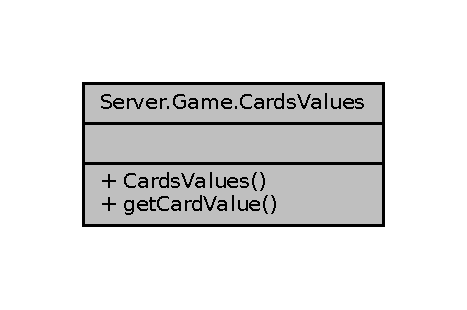
\includegraphics[width=224pt]{classServer_1_1Game_1_1CardsValues__coll__graph}
\end{center}
\end{figure}
\subsection*{Public Member Functions}
\begin{DoxyCompactItemize}
\item 
\mbox{\hyperlink{classServer_1_1Game_1_1CardsValues_a634d4777af4a21205f3ca33caa22e958}{Cards\+Values}} ()
\item 
int \mbox{\hyperlink{classServer_1_1Game_1_1CardsValues_a9565f977853cc769004d989b3f9524c6}{get\+Card\+Value}} (\mbox{\hyperlink{classCommon_1_1Card}{Card}} card, boolean is\+Trump)
\end{DoxyCompactItemize}


\subsection{Constructor \& Destructor Documentation}
\mbox{\Hypertarget{classServer_1_1Game_1_1CardsValues_a634d4777af4a21205f3ca33caa22e958}\label{classServer_1_1Game_1_1CardsValues_a634d4777af4a21205f3ca33caa22e958}} 
\index{Server\+::\+Game\+::\+Cards\+Values@{Server\+::\+Game\+::\+Cards\+Values}!Cards\+Values@{Cards\+Values}}
\index{Cards\+Values@{Cards\+Values}!Server\+::\+Game\+::\+Cards\+Values@{Server\+::\+Game\+::\+Cards\+Values}}
\subsubsection{\texorpdfstring{Cards\+Values()}{CardsValues()}}
{\footnotesize\ttfamily Server.\+Game.\+Cards\+Values.\+Cards\+Values (\begin{DoxyParamCaption}{ }\end{DoxyParamCaption})\hspace{0.3cm}{\ttfamily [inline]}}



\subsection{Member Function Documentation}
\mbox{\Hypertarget{classServer_1_1Game_1_1CardsValues_a9565f977853cc769004d989b3f9524c6}\label{classServer_1_1Game_1_1CardsValues_a9565f977853cc769004d989b3f9524c6}} 
\index{Server\+::\+Game\+::\+Cards\+Values@{Server\+::\+Game\+::\+Cards\+Values}!get\+Card\+Value@{get\+Card\+Value}}
\index{get\+Card\+Value@{get\+Card\+Value}!Server\+::\+Game\+::\+Cards\+Values@{Server\+::\+Game\+::\+Cards\+Values}}
\subsubsection{\texorpdfstring{get\+Card\+Value()}{getCardValue()}}
{\footnotesize\ttfamily int Server.\+Game.\+Cards\+Values.\+get\+Card\+Value (\begin{DoxyParamCaption}\item[{\mbox{\hyperlink{classCommon_1_1Card}{Card}}}]{card,  }\item[{boolean}]{is\+Trump }\end{DoxyParamCaption})\hspace{0.3cm}{\ttfamily [inline]}}



The documentation for this class was generated from the following file\+:\begin{DoxyCompactItemize}
\item 
/home/tetard/\+Idea\+Projects/j\+Coinche/\+Java\+\_\+jcoinche\+\_\+2017/src/main/java/\+Server/\+Game/\mbox{\hyperlink{CardsValues_8java}{Cards\+Values.\+java}}\end{DoxyCompactItemize}

\hypertarget{classClient_1_1NetWork_1_1ClientConnection}{}\section{Client.\+Net\+Work.\+Client\+Connection Class Reference}
\label{classClient_1_1NetWork_1_1ClientConnection}\index{Client.\+Net\+Work.\+Client\+Connection@{Client.\+Net\+Work.\+Client\+Connection}}


Collaboration diagram for Client.\+Net\+Work.\+Client\+Connection\+:
\nopagebreak
\begin{figure}[H]
\begin{center}
\leavevmode
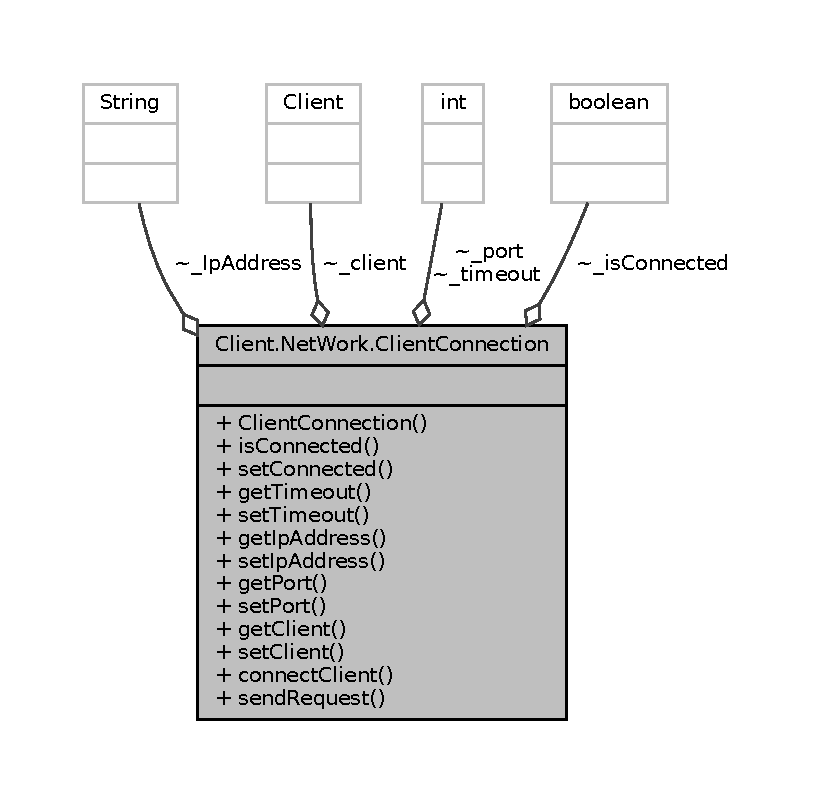
\includegraphics[width=350pt]{classClient_1_1NetWork_1_1ClientConnection__coll__graph}
\end{center}
\end{figure}
\subsection*{Public Member Functions}
\begin{DoxyCompactItemize}
\item 
\mbox{\hyperlink{classClient_1_1NetWork_1_1ClientConnection_ab769ef42a838b10b9415084ee7addeab}{Client\+Connection}} (int timeout, String ip\+Address, int port)  throws I\+O\+Exception 
\item 
boolean \mbox{\hyperlink{classClient_1_1NetWork_1_1ClientConnection_a5783f46666a7c84bbb3204931909fc1d}{is\+Connected}} ()
\item 
void \mbox{\hyperlink{classClient_1_1NetWork_1_1ClientConnection_a34be6fb246319ec8f2aa6ee5b6b3e428}{set\+Connected}} (boolean connected)
\item 
int \mbox{\hyperlink{classClient_1_1NetWork_1_1ClientConnection_abe7fc9290de73d965518dd9de09cd409}{get\+Timeout}} ()
\item 
void \mbox{\hyperlink{classClient_1_1NetWork_1_1ClientConnection_ab8a2ea55eded25fb292ae13cef965100}{set\+Timeout}} (int timeout)
\item 
String \mbox{\hyperlink{classClient_1_1NetWork_1_1ClientConnection_a4d0ee3c2ffe3f39cc8e730303606668b}{get\+Ip\+Address}} ()
\item 
void \mbox{\hyperlink{classClient_1_1NetWork_1_1ClientConnection_a8651f578e4701a3de7cf4d158aa4a25f}{set\+Ip\+Address}} (String Ip\+Address)
\item 
int \mbox{\hyperlink{classClient_1_1NetWork_1_1ClientConnection_aa469697b3b88fb6c55947a2bd86a1bce}{get\+Port}} ()
\item 
void \mbox{\hyperlink{classClient_1_1NetWork_1_1ClientConnection_abc5ca369107ad809258d23af01dcf959}{set\+Port}} (int port)
\item 
Client \mbox{\hyperlink{classClient_1_1NetWork_1_1ClientConnection_a68b1b929e307664e06ae49c5535b4f8e}{get\+Client}} ()
\item 
void \mbox{\hyperlink{classClient_1_1NetWork_1_1ClientConnection_a9778327e17e67da3b47451a95c00b4b0}{set\+Client}} (Client client)
\item 
void \mbox{\hyperlink{classClient_1_1NetWork_1_1ClientConnection_a39110498a3fd58e5ddc40b59358fcd94}{connect\+Client}} ()  throws I\+O\+Exception 
\item 
void \mbox{\hyperlink{classClient_1_1NetWork_1_1ClientConnection_aef871fa6a2b3a81d43d6a0b99a538581}{send\+Request}} (Object obj)
\end{DoxyCompactItemize}


\subsection{Constructor \& Destructor Documentation}
\mbox{\Hypertarget{classClient_1_1NetWork_1_1ClientConnection_ab769ef42a838b10b9415084ee7addeab}\label{classClient_1_1NetWork_1_1ClientConnection_ab769ef42a838b10b9415084ee7addeab}} 
\index{Client\+::\+Net\+Work\+::\+Client\+Connection@{Client\+::\+Net\+Work\+::\+Client\+Connection}!Client\+Connection@{Client\+Connection}}
\index{Client\+Connection@{Client\+Connection}!Client\+::\+Net\+Work\+::\+Client\+Connection@{Client\+::\+Net\+Work\+::\+Client\+Connection}}
\subsubsection{\texorpdfstring{Client\+Connection()}{ClientConnection()}}
{\footnotesize\ttfamily Client.\+Net\+Work.\+Client\+Connection.\+Client\+Connection (\begin{DoxyParamCaption}\item[{int}]{timeout,  }\item[{String}]{ip\+Address,  }\item[{int}]{port }\end{DoxyParamCaption}) throws I\+O\+Exception\hspace{0.3cm}{\ttfamily [inline]}}



\subsection{Member Function Documentation}
\mbox{\Hypertarget{classClient_1_1NetWork_1_1ClientConnection_a39110498a3fd58e5ddc40b59358fcd94}\label{classClient_1_1NetWork_1_1ClientConnection_a39110498a3fd58e5ddc40b59358fcd94}} 
\index{Client\+::\+Net\+Work\+::\+Client\+Connection@{Client\+::\+Net\+Work\+::\+Client\+Connection}!connect\+Client@{connect\+Client}}
\index{connect\+Client@{connect\+Client}!Client\+::\+Net\+Work\+::\+Client\+Connection@{Client\+::\+Net\+Work\+::\+Client\+Connection}}
\subsubsection{\texorpdfstring{connect\+Client()}{connectClient()}}
{\footnotesize\ttfamily void Client.\+Net\+Work.\+Client\+Connection.\+connect\+Client (\begin{DoxyParamCaption}{ }\end{DoxyParamCaption}) throws I\+O\+Exception\hspace{0.3cm}{\ttfamily [inline]}}

\mbox{\Hypertarget{classClient_1_1NetWork_1_1ClientConnection_a68b1b929e307664e06ae49c5535b4f8e}\label{classClient_1_1NetWork_1_1ClientConnection_a68b1b929e307664e06ae49c5535b4f8e}} 
\index{Client\+::\+Net\+Work\+::\+Client\+Connection@{Client\+::\+Net\+Work\+::\+Client\+Connection}!get\+Client@{get\+Client}}
\index{get\+Client@{get\+Client}!Client\+::\+Net\+Work\+::\+Client\+Connection@{Client\+::\+Net\+Work\+::\+Client\+Connection}}
\subsubsection{\texorpdfstring{get\+Client()}{getClient()}}
{\footnotesize\ttfamily Client Client.\+Net\+Work.\+Client\+Connection.\+get\+Client (\begin{DoxyParamCaption}{ }\end{DoxyParamCaption})\hspace{0.3cm}{\ttfamily [inline]}}

\mbox{\Hypertarget{classClient_1_1NetWork_1_1ClientConnection_a4d0ee3c2ffe3f39cc8e730303606668b}\label{classClient_1_1NetWork_1_1ClientConnection_a4d0ee3c2ffe3f39cc8e730303606668b}} 
\index{Client\+::\+Net\+Work\+::\+Client\+Connection@{Client\+::\+Net\+Work\+::\+Client\+Connection}!get\+Ip\+Address@{get\+Ip\+Address}}
\index{get\+Ip\+Address@{get\+Ip\+Address}!Client\+::\+Net\+Work\+::\+Client\+Connection@{Client\+::\+Net\+Work\+::\+Client\+Connection}}
\subsubsection{\texorpdfstring{get\+Ip\+Address()}{getIpAddress()}}
{\footnotesize\ttfamily String Client.\+Net\+Work.\+Client\+Connection.\+get\+Ip\+Address (\begin{DoxyParamCaption}{ }\end{DoxyParamCaption})\hspace{0.3cm}{\ttfamily [inline]}}

\mbox{\Hypertarget{classClient_1_1NetWork_1_1ClientConnection_aa469697b3b88fb6c55947a2bd86a1bce}\label{classClient_1_1NetWork_1_1ClientConnection_aa469697b3b88fb6c55947a2bd86a1bce}} 
\index{Client\+::\+Net\+Work\+::\+Client\+Connection@{Client\+::\+Net\+Work\+::\+Client\+Connection}!get\+Port@{get\+Port}}
\index{get\+Port@{get\+Port}!Client\+::\+Net\+Work\+::\+Client\+Connection@{Client\+::\+Net\+Work\+::\+Client\+Connection}}
\subsubsection{\texorpdfstring{get\+Port()}{getPort()}}
{\footnotesize\ttfamily int Client.\+Net\+Work.\+Client\+Connection.\+get\+Port (\begin{DoxyParamCaption}{ }\end{DoxyParamCaption})\hspace{0.3cm}{\ttfamily [inline]}}

\mbox{\Hypertarget{classClient_1_1NetWork_1_1ClientConnection_abe7fc9290de73d965518dd9de09cd409}\label{classClient_1_1NetWork_1_1ClientConnection_abe7fc9290de73d965518dd9de09cd409}} 
\index{Client\+::\+Net\+Work\+::\+Client\+Connection@{Client\+::\+Net\+Work\+::\+Client\+Connection}!get\+Timeout@{get\+Timeout}}
\index{get\+Timeout@{get\+Timeout}!Client\+::\+Net\+Work\+::\+Client\+Connection@{Client\+::\+Net\+Work\+::\+Client\+Connection}}
\subsubsection{\texorpdfstring{get\+Timeout()}{getTimeout()}}
{\footnotesize\ttfamily int Client.\+Net\+Work.\+Client\+Connection.\+get\+Timeout (\begin{DoxyParamCaption}{ }\end{DoxyParamCaption})\hspace{0.3cm}{\ttfamily [inline]}}

\mbox{\Hypertarget{classClient_1_1NetWork_1_1ClientConnection_a5783f46666a7c84bbb3204931909fc1d}\label{classClient_1_1NetWork_1_1ClientConnection_a5783f46666a7c84bbb3204931909fc1d}} 
\index{Client\+::\+Net\+Work\+::\+Client\+Connection@{Client\+::\+Net\+Work\+::\+Client\+Connection}!is\+Connected@{is\+Connected}}
\index{is\+Connected@{is\+Connected}!Client\+::\+Net\+Work\+::\+Client\+Connection@{Client\+::\+Net\+Work\+::\+Client\+Connection}}
\subsubsection{\texorpdfstring{is\+Connected()}{isConnected()}}
{\footnotesize\ttfamily boolean Client.\+Net\+Work.\+Client\+Connection.\+is\+Connected (\begin{DoxyParamCaption}{ }\end{DoxyParamCaption})\hspace{0.3cm}{\ttfamily [inline]}}

\mbox{\Hypertarget{classClient_1_1NetWork_1_1ClientConnection_aef871fa6a2b3a81d43d6a0b99a538581}\label{classClient_1_1NetWork_1_1ClientConnection_aef871fa6a2b3a81d43d6a0b99a538581}} 
\index{Client\+::\+Net\+Work\+::\+Client\+Connection@{Client\+::\+Net\+Work\+::\+Client\+Connection}!send\+Request@{send\+Request}}
\index{send\+Request@{send\+Request}!Client\+::\+Net\+Work\+::\+Client\+Connection@{Client\+::\+Net\+Work\+::\+Client\+Connection}}
\subsubsection{\texorpdfstring{send\+Request()}{sendRequest()}}
{\footnotesize\ttfamily void Client.\+Net\+Work.\+Client\+Connection.\+send\+Request (\begin{DoxyParamCaption}\item[{Object}]{obj }\end{DoxyParamCaption})\hspace{0.3cm}{\ttfamily [inline]}}

\mbox{\Hypertarget{classClient_1_1NetWork_1_1ClientConnection_a9778327e17e67da3b47451a95c00b4b0}\label{classClient_1_1NetWork_1_1ClientConnection_a9778327e17e67da3b47451a95c00b4b0}} 
\index{Client\+::\+Net\+Work\+::\+Client\+Connection@{Client\+::\+Net\+Work\+::\+Client\+Connection}!set\+Client@{set\+Client}}
\index{set\+Client@{set\+Client}!Client\+::\+Net\+Work\+::\+Client\+Connection@{Client\+::\+Net\+Work\+::\+Client\+Connection}}
\subsubsection{\texorpdfstring{set\+Client()}{setClient()}}
{\footnotesize\ttfamily void Client.\+Net\+Work.\+Client\+Connection.\+set\+Client (\begin{DoxyParamCaption}\item[{Client}]{client }\end{DoxyParamCaption})\hspace{0.3cm}{\ttfamily [inline]}}

\mbox{\Hypertarget{classClient_1_1NetWork_1_1ClientConnection_a34be6fb246319ec8f2aa6ee5b6b3e428}\label{classClient_1_1NetWork_1_1ClientConnection_a34be6fb246319ec8f2aa6ee5b6b3e428}} 
\index{Client\+::\+Net\+Work\+::\+Client\+Connection@{Client\+::\+Net\+Work\+::\+Client\+Connection}!set\+Connected@{set\+Connected}}
\index{set\+Connected@{set\+Connected}!Client\+::\+Net\+Work\+::\+Client\+Connection@{Client\+::\+Net\+Work\+::\+Client\+Connection}}
\subsubsection{\texorpdfstring{set\+Connected()}{setConnected()}}
{\footnotesize\ttfamily void Client.\+Net\+Work.\+Client\+Connection.\+set\+Connected (\begin{DoxyParamCaption}\item[{boolean}]{connected }\end{DoxyParamCaption})\hspace{0.3cm}{\ttfamily [inline]}}

\mbox{\Hypertarget{classClient_1_1NetWork_1_1ClientConnection_a8651f578e4701a3de7cf4d158aa4a25f}\label{classClient_1_1NetWork_1_1ClientConnection_a8651f578e4701a3de7cf4d158aa4a25f}} 
\index{Client\+::\+Net\+Work\+::\+Client\+Connection@{Client\+::\+Net\+Work\+::\+Client\+Connection}!set\+Ip\+Address@{set\+Ip\+Address}}
\index{set\+Ip\+Address@{set\+Ip\+Address}!Client\+::\+Net\+Work\+::\+Client\+Connection@{Client\+::\+Net\+Work\+::\+Client\+Connection}}
\subsubsection{\texorpdfstring{set\+Ip\+Address()}{setIpAddress()}}
{\footnotesize\ttfamily void Client.\+Net\+Work.\+Client\+Connection.\+set\+Ip\+Address (\begin{DoxyParamCaption}\item[{String}]{Ip\+Address }\end{DoxyParamCaption})\hspace{0.3cm}{\ttfamily [inline]}}

\mbox{\Hypertarget{classClient_1_1NetWork_1_1ClientConnection_abc5ca369107ad809258d23af01dcf959}\label{classClient_1_1NetWork_1_1ClientConnection_abc5ca369107ad809258d23af01dcf959}} 
\index{Client\+::\+Net\+Work\+::\+Client\+Connection@{Client\+::\+Net\+Work\+::\+Client\+Connection}!set\+Port@{set\+Port}}
\index{set\+Port@{set\+Port}!Client\+::\+Net\+Work\+::\+Client\+Connection@{Client\+::\+Net\+Work\+::\+Client\+Connection}}
\subsubsection{\texorpdfstring{set\+Port()}{setPort()}}
{\footnotesize\ttfamily void Client.\+Net\+Work.\+Client\+Connection.\+set\+Port (\begin{DoxyParamCaption}\item[{int}]{port }\end{DoxyParamCaption})\hspace{0.3cm}{\ttfamily [inline]}}

\mbox{\Hypertarget{classClient_1_1NetWork_1_1ClientConnection_ab8a2ea55eded25fb292ae13cef965100}\label{classClient_1_1NetWork_1_1ClientConnection_ab8a2ea55eded25fb292ae13cef965100}} 
\index{Client\+::\+Net\+Work\+::\+Client\+Connection@{Client\+::\+Net\+Work\+::\+Client\+Connection}!set\+Timeout@{set\+Timeout}}
\index{set\+Timeout@{set\+Timeout}!Client\+::\+Net\+Work\+::\+Client\+Connection@{Client\+::\+Net\+Work\+::\+Client\+Connection}}
\subsubsection{\texorpdfstring{set\+Timeout()}{setTimeout()}}
{\footnotesize\ttfamily void Client.\+Net\+Work.\+Client\+Connection.\+set\+Timeout (\begin{DoxyParamCaption}\item[{int}]{timeout }\end{DoxyParamCaption})\hspace{0.3cm}{\ttfamily [inline]}}



The documentation for this class was generated from the following file\+:\begin{DoxyCompactItemize}
\item 
/home/tetard/\+Idea\+Projects/j\+Coinche/\+Java\+\_\+jcoinche\+\_\+2017/src/main/java/\+Client/\+Net\+Work/\mbox{\hyperlink{ClientConnection_8java}{Client\+Connection.\+java}}\end{DoxyCompactItemize}

\hypertarget{classServer_1_1ServerConnexion_1_1ClientInfos}{}\section{Server.\+Server\+Connexion.\+Client\+Infos Class Reference}
\label{classServer_1_1ServerConnexion_1_1ClientInfos}\index{Server.\+Server\+Connexion.\+Client\+Infos@{Server.\+Server\+Connexion.\+Client\+Infos}}


Collaboration diagram for Server.\+Server\+Connexion.\+Client\+Infos\+:
\nopagebreak
\begin{figure}[H]
\begin{center}
\leavevmode
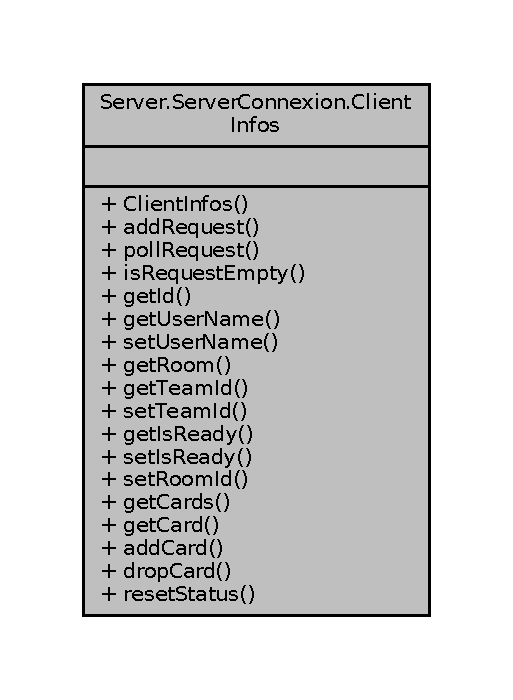
\includegraphics[width=246pt]{classServer_1_1ServerConnexion_1_1ClientInfos__coll__graph}
\end{center}
\end{figure}
\subsection*{Public Member Functions}
\begin{DoxyCompactItemize}
\item 
\mbox{\hyperlink{classServer_1_1ServerConnexion_1_1ClientInfos_a970d91293292cf6f463e532dc69734cf}{Client\+Infos}} (int id)
\item 
void \mbox{\hyperlink{classServer_1_1ServerConnexion_1_1ClientInfos_a50227a4e9e1c8210b77183e90119ae8e}{add\+Request}} (Object request)
\item 
Object \mbox{\hyperlink{classServer_1_1ServerConnexion_1_1ClientInfos_a6b62e65651d69cea2fde466c77bcf8b2}{poll\+Request}} ()
\item 
boolean \mbox{\hyperlink{classServer_1_1ServerConnexion_1_1ClientInfos_a524923ad3071663acb7dfba9d42e20a2}{is\+Request\+Empty}} ()
\item 
int \mbox{\hyperlink{classServer_1_1ServerConnexion_1_1ClientInfos_a10ffde5dcae701e2d279ed93854433c4}{get\+Id}} ()
\item 
String \mbox{\hyperlink{classServer_1_1ServerConnexion_1_1ClientInfos_a6614d5ebe7b522247006a2c89e7e3333}{get\+User\+Name}} ()
\item 
void \mbox{\hyperlink{classServer_1_1ServerConnexion_1_1ClientInfos_a7b48005e4d20338b8e0c952827111bf0}{set\+User\+Name}} (String user\+Name)
\item 
int \mbox{\hyperlink{classServer_1_1ServerConnexion_1_1ClientInfos_ad545432f341ce38c57e341617366361f}{get\+Room}} ()
\item 
int \mbox{\hyperlink{classServer_1_1ServerConnexion_1_1ClientInfos_a18960a701432d548bc20fc1955dbd154}{get\+Team\+Id}} ()
\item 
void \mbox{\hyperlink{classServer_1_1ServerConnexion_1_1ClientInfos_a6732e1179ce660c6c874053d82136498}{set\+Team\+Id}} (int team\+Id)
\item 
boolean \mbox{\hyperlink{classServer_1_1ServerConnexion_1_1ClientInfos_a871e9ffff7d78ef66257cb69974af05c}{get\+Is\+Ready}} ()
\item 
void \mbox{\hyperlink{classServer_1_1ServerConnexion_1_1ClientInfos_a4f001fc33e2fef60c5fbbb7f7ffce9c3}{set\+Is\+Ready}} (boolean is\+Ready)
\item 
void \mbox{\hyperlink{classServer_1_1ServerConnexion_1_1ClientInfos_a98c355362aabfa1b4fdc1a5ab108c6d0}{set\+Room\+Id}} (int room)
\item 
Hash\+Map$<$ Integer, \mbox{\hyperlink{classCommon_1_1Card}{Card}} $>$ \mbox{\hyperlink{classServer_1_1ServerConnexion_1_1ClientInfos_a3ae6c7e00203eb9468ba54f32707baf5}{get\+Cards}} ()
\item 
\mbox{\hyperlink{classCommon_1_1Card}{Card}} \mbox{\hyperlink{classServer_1_1ServerConnexion_1_1ClientInfos_a59f88a0546f6dbc1debbf59482144332}{get\+Card}} (int id)
\item 
void \mbox{\hyperlink{classServer_1_1ServerConnexion_1_1ClientInfos_a7c773a28b6464e2ed8e9864bfc5793cb}{add\+Card}} (\mbox{\hyperlink{classCommon_1_1Card}{Card}} card)
\item 
\mbox{\hyperlink{classCommon_1_1Card}{Card}} \mbox{\hyperlink{classServer_1_1ServerConnexion_1_1ClientInfos_af561becca2a435a2190dc945949f524d}{drop\+Card}} (int id)
\item 
void \mbox{\hyperlink{classServer_1_1ServerConnexion_1_1ClientInfos_a7dee6a06e3869026da38c0e7d1b9e2b6}{reset\+Status}} ()
\end{DoxyCompactItemize}


\subsection{Constructor \& Destructor Documentation}
\mbox{\Hypertarget{classServer_1_1ServerConnexion_1_1ClientInfos_a970d91293292cf6f463e532dc69734cf}\label{classServer_1_1ServerConnexion_1_1ClientInfos_a970d91293292cf6f463e532dc69734cf}} 
\index{Server\+::\+Server\+Connexion\+::\+Client\+Infos@{Server\+::\+Server\+Connexion\+::\+Client\+Infos}!Client\+Infos@{Client\+Infos}}
\index{Client\+Infos@{Client\+Infos}!Server\+::\+Server\+Connexion\+::\+Client\+Infos@{Server\+::\+Server\+Connexion\+::\+Client\+Infos}}
\subsubsection{\texorpdfstring{Client\+Infos()}{ClientInfos()}}
{\footnotesize\ttfamily Server.\+Server\+Connexion.\+Client\+Infos.\+Client\+Infos (\begin{DoxyParamCaption}\item[{int}]{id }\end{DoxyParamCaption})\hspace{0.3cm}{\ttfamily [inline]}}



\subsection{Member Function Documentation}
\mbox{\Hypertarget{classServer_1_1ServerConnexion_1_1ClientInfos_a7c773a28b6464e2ed8e9864bfc5793cb}\label{classServer_1_1ServerConnexion_1_1ClientInfos_a7c773a28b6464e2ed8e9864bfc5793cb}} 
\index{Server\+::\+Server\+Connexion\+::\+Client\+Infos@{Server\+::\+Server\+Connexion\+::\+Client\+Infos}!add\+Card@{add\+Card}}
\index{add\+Card@{add\+Card}!Server\+::\+Server\+Connexion\+::\+Client\+Infos@{Server\+::\+Server\+Connexion\+::\+Client\+Infos}}
\subsubsection{\texorpdfstring{add\+Card()}{addCard()}}
{\footnotesize\ttfamily void Server.\+Server\+Connexion.\+Client\+Infos.\+add\+Card (\begin{DoxyParamCaption}\item[{\mbox{\hyperlink{classCommon_1_1Card}{Card}}}]{card }\end{DoxyParamCaption})\hspace{0.3cm}{\ttfamily [inline]}}

\mbox{\Hypertarget{classServer_1_1ServerConnexion_1_1ClientInfos_a50227a4e9e1c8210b77183e90119ae8e}\label{classServer_1_1ServerConnexion_1_1ClientInfos_a50227a4e9e1c8210b77183e90119ae8e}} 
\index{Server\+::\+Server\+Connexion\+::\+Client\+Infos@{Server\+::\+Server\+Connexion\+::\+Client\+Infos}!add\+Request@{add\+Request}}
\index{add\+Request@{add\+Request}!Server\+::\+Server\+Connexion\+::\+Client\+Infos@{Server\+::\+Server\+Connexion\+::\+Client\+Infos}}
\subsubsection{\texorpdfstring{add\+Request()}{addRequest()}}
{\footnotesize\ttfamily void Server.\+Server\+Connexion.\+Client\+Infos.\+add\+Request (\begin{DoxyParamCaption}\item[{Object}]{request }\end{DoxyParamCaption})\hspace{0.3cm}{\ttfamily [inline]}}

\mbox{\Hypertarget{classServer_1_1ServerConnexion_1_1ClientInfos_af561becca2a435a2190dc945949f524d}\label{classServer_1_1ServerConnexion_1_1ClientInfos_af561becca2a435a2190dc945949f524d}} 
\index{Server\+::\+Server\+Connexion\+::\+Client\+Infos@{Server\+::\+Server\+Connexion\+::\+Client\+Infos}!drop\+Card@{drop\+Card}}
\index{drop\+Card@{drop\+Card}!Server\+::\+Server\+Connexion\+::\+Client\+Infos@{Server\+::\+Server\+Connexion\+::\+Client\+Infos}}
\subsubsection{\texorpdfstring{drop\+Card()}{dropCard()}}
{\footnotesize\ttfamily \mbox{\hyperlink{classCommon_1_1Card}{Card}} Server.\+Server\+Connexion.\+Client\+Infos.\+drop\+Card (\begin{DoxyParamCaption}\item[{int}]{id }\end{DoxyParamCaption})\hspace{0.3cm}{\ttfamily [inline]}}

\mbox{\Hypertarget{classServer_1_1ServerConnexion_1_1ClientInfos_a59f88a0546f6dbc1debbf59482144332}\label{classServer_1_1ServerConnexion_1_1ClientInfos_a59f88a0546f6dbc1debbf59482144332}} 
\index{Server\+::\+Server\+Connexion\+::\+Client\+Infos@{Server\+::\+Server\+Connexion\+::\+Client\+Infos}!get\+Card@{get\+Card}}
\index{get\+Card@{get\+Card}!Server\+::\+Server\+Connexion\+::\+Client\+Infos@{Server\+::\+Server\+Connexion\+::\+Client\+Infos}}
\subsubsection{\texorpdfstring{get\+Card()}{getCard()}}
{\footnotesize\ttfamily \mbox{\hyperlink{classCommon_1_1Card}{Card}} Server.\+Server\+Connexion.\+Client\+Infos.\+get\+Card (\begin{DoxyParamCaption}\item[{int}]{id }\end{DoxyParamCaption})\hspace{0.3cm}{\ttfamily [inline]}}

\mbox{\Hypertarget{classServer_1_1ServerConnexion_1_1ClientInfos_a3ae6c7e00203eb9468ba54f32707baf5}\label{classServer_1_1ServerConnexion_1_1ClientInfos_a3ae6c7e00203eb9468ba54f32707baf5}} 
\index{Server\+::\+Server\+Connexion\+::\+Client\+Infos@{Server\+::\+Server\+Connexion\+::\+Client\+Infos}!get\+Cards@{get\+Cards}}
\index{get\+Cards@{get\+Cards}!Server\+::\+Server\+Connexion\+::\+Client\+Infos@{Server\+::\+Server\+Connexion\+::\+Client\+Infos}}
\subsubsection{\texorpdfstring{get\+Cards()}{getCards()}}
{\footnotesize\ttfamily Hash\+Map$<$Integer, \mbox{\hyperlink{classCommon_1_1Card}{Card}}$>$ Server.\+Server\+Connexion.\+Client\+Infos.\+get\+Cards (\begin{DoxyParamCaption}{ }\end{DoxyParamCaption})\hspace{0.3cm}{\ttfamily [inline]}}

\mbox{\Hypertarget{classServer_1_1ServerConnexion_1_1ClientInfos_a10ffde5dcae701e2d279ed93854433c4}\label{classServer_1_1ServerConnexion_1_1ClientInfos_a10ffde5dcae701e2d279ed93854433c4}} 
\index{Server\+::\+Server\+Connexion\+::\+Client\+Infos@{Server\+::\+Server\+Connexion\+::\+Client\+Infos}!get\+Id@{get\+Id}}
\index{get\+Id@{get\+Id}!Server\+::\+Server\+Connexion\+::\+Client\+Infos@{Server\+::\+Server\+Connexion\+::\+Client\+Infos}}
\subsubsection{\texorpdfstring{get\+Id()}{getId()}}
{\footnotesize\ttfamily int Server.\+Server\+Connexion.\+Client\+Infos.\+get\+Id (\begin{DoxyParamCaption}{ }\end{DoxyParamCaption})\hspace{0.3cm}{\ttfamily [inline]}}

\mbox{\Hypertarget{classServer_1_1ServerConnexion_1_1ClientInfos_a871e9ffff7d78ef66257cb69974af05c}\label{classServer_1_1ServerConnexion_1_1ClientInfos_a871e9ffff7d78ef66257cb69974af05c}} 
\index{Server\+::\+Server\+Connexion\+::\+Client\+Infos@{Server\+::\+Server\+Connexion\+::\+Client\+Infos}!get\+Is\+Ready@{get\+Is\+Ready}}
\index{get\+Is\+Ready@{get\+Is\+Ready}!Server\+::\+Server\+Connexion\+::\+Client\+Infos@{Server\+::\+Server\+Connexion\+::\+Client\+Infos}}
\subsubsection{\texorpdfstring{get\+Is\+Ready()}{getIsReady()}}
{\footnotesize\ttfamily boolean Server.\+Server\+Connexion.\+Client\+Infos.\+get\+Is\+Ready (\begin{DoxyParamCaption}{ }\end{DoxyParamCaption})\hspace{0.3cm}{\ttfamily [inline]}}

\mbox{\Hypertarget{classServer_1_1ServerConnexion_1_1ClientInfos_ad545432f341ce38c57e341617366361f}\label{classServer_1_1ServerConnexion_1_1ClientInfos_ad545432f341ce38c57e341617366361f}} 
\index{Server\+::\+Server\+Connexion\+::\+Client\+Infos@{Server\+::\+Server\+Connexion\+::\+Client\+Infos}!get\+Room@{get\+Room}}
\index{get\+Room@{get\+Room}!Server\+::\+Server\+Connexion\+::\+Client\+Infos@{Server\+::\+Server\+Connexion\+::\+Client\+Infos}}
\subsubsection{\texorpdfstring{get\+Room()}{getRoom()}}
{\footnotesize\ttfamily int Server.\+Server\+Connexion.\+Client\+Infos.\+get\+Room (\begin{DoxyParamCaption}{ }\end{DoxyParamCaption})\hspace{0.3cm}{\ttfamily [inline]}}

\mbox{\Hypertarget{classServer_1_1ServerConnexion_1_1ClientInfos_a18960a701432d548bc20fc1955dbd154}\label{classServer_1_1ServerConnexion_1_1ClientInfos_a18960a701432d548bc20fc1955dbd154}} 
\index{Server\+::\+Server\+Connexion\+::\+Client\+Infos@{Server\+::\+Server\+Connexion\+::\+Client\+Infos}!get\+Team\+Id@{get\+Team\+Id}}
\index{get\+Team\+Id@{get\+Team\+Id}!Server\+::\+Server\+Connexion\+::\+Client\+Infos@{Server\+::\+Server\+Connexion\+::\+Client\+Infos}}
\subsubsection{\texorpdfstring{get\+Team\+Id()}{getTeamId()}}
{\footnotesize\ttfamily int Server.\+Server\+Connexion.\+Client\+Infos.\+get\+Team\+Id (\begin{DoxyParamCaption}{ }\end{DoxyParamCaption})\hspace{0.3cm}{\ttfamily [inline]}}

\mbox{\Hypertarget{classServer_1_1ServerConnexion_1_1ClientInfos_a6614d5ebe7b522247006a2c89e7e3333}\label{classServer_1_1ServerConnexion_1_1ClientInfos_a6614d5ebe7b522247006a2c89e7e3333}} 
\index{Server\+::\+Server\+Connexion\+::\+Client\+Infos@{Server\+::\+Server\+Connexion\+::\+Client\+Infos}!get\+User\+Name@{get\+User\+Name}}
\index{get\+User\+Name@{get\+User\+Name}!Server\+::\+Server\+Connexion\+::\+Client\+Infos@{Server\+::\+Server\+Connexion\+::\+Client\+Infos}}
\subsubsection{\texorpdfstring{get\+User\+Name()}{getUserName()}}
{\footnotesize\ttfamily String Server.\+Server\+Connexion.\+Client\+Infos.\+get\+User\+Name (\begin{DoxyParamCaption}{ }\end{DoxyParamCaption})\hspace{0.3cm}{\ttfamily [inline]}}

\mbox{\Hypertarget{classServer_1_1ServerConnexion_1_1ClientInfos_a524923ad3071663acb7dfba9d42e20a2}\label{classServer_1_1ServerConnexion_1_1ClientInfos_a524923ad3071663acb7dfba9d42e20a2}} 
\index{Server\+::\+Server\+Connexion\+::\+Client\+Infos@{Server\+::\+Server\+Connexion\+::\+Client\+Infos}!is\+Request\+Empty@{is\+Request\+Empty}}
\index{is\+Request\+Empty@{is\+Request\+Empty}!Server\+::\+Server\+Connexion\+::\+Client\+Infos@{Server\+::\+Server\+Connexion\+::\+Client\+Infos}}
\subsubsection{\texorpdfstring{is\+Request\+Empty()}{isRequestEmpty()}}
{\footnotesize\ttfamily boolean Server.\+Server\+Connexion.\+Client\+Infos.\+is\+Request\+Empty (\begin{DoxyParamCaption}{ }\end{DoxyParamCaption})\hspace{0.3cm}{\ttfamily [inline]}}

\mbox{\Hypertarget{classServer_1_1ServerConnexion_1_1ClientInfos_a6b62e65651d69cea2fde466c77bcf8b2}\label{classServer_1_1ServerConnexion_1_1ClientInfos_a6b62e65651d69cea2fde466c77bcf8b2}} 
\index{Server\+::\+Server\+Connexion\+::\+Client\+Infos@{Server\+::\+Server\+Connexion\+::\+Client\+Infos}!poll\+Request@{poll\+Request}}
\index{poll\+Request@{poll\+Request}!Server\+::\+Server\+Connexion\+::\+Client\+Infos@{Server\+::\+Server\+Connexion\+::\+Client\+Infos}}
\subsubsection{\texorpdfstring{poll\+Request()}{pollRequest()}}
{\footnotesize\ttfamily Object Server.\+Server\+Connexion.\+Client\+Infos.\+poll\+Request (\begin{DoxyParamCaption}{ }\end{DoxyParamCaption})\hspace{0.3cm}{\ttfamily [inline]}}

\mbox{\Hypertarget{classServer_1_1ServerConnexion_1_1ClientInfos_a7dee6a06e3869026da38c0e7d1b9e2b6}\label{classServer_1_1ServerConnexion_1_1ClientInfos_a7dee6a06e3869026da38c0e7d1b9e2b6}} 
\index{Server\+::\+Server\+Connexion\+::\+Client\+Infos@{Server\+::\+Server\+Connexion\+::\+Client\+Infos}!reset\+Status@{reset\+Status}}
\index{reset\+Status@{reset\+Status}!Server\+::\+Server\+Connexion\+::\+Client\+Infos@{Server\+::\+Server\+Connexion\+::\+Client\+Infos}}
\subsubsection{\texorpdfstring{reset\+Status()}{resetStatus()}}
{\footnotesize\ttfamily void Server.\+Server\+Connexion.\+Client\+Infos.\+reset\+Status (\begin{DoxyParamCaption}{ }\end{DoxyParamCaption})\hspace{0.3cm}{\ttfamily [inline]}}

\mbox{\Hypertarget{classServer_1_1ServerConnexion_1_1ClientInfos_a4f001fc33e2fef60c5fbbb7f7ffce9c3}\label{classServer_1_1ServerConnexion_1_1ClientInfos_a4f001fc33e2fef60c5fbbb7f7ffce9c3}} 
\index{Server\+::\+Server\+Connexion\+::\+Client\+Infos@{Server\+::\+Server\+Connexion\+::\+Client\+Infos}!set\+Is\+Ready@{set\+Is\+Ready}}
\index{set\+Is\+Ready@{set\+Is\+Ready}!Server\+::\+Server\+Connexion\+::\+Client\+Infos@{Server\+::\+Server\+Connexion\+::\+Client\+Infos}}
\subsubsection{\texorpdfstring{set\+Is\+Ready()}{setIsReady()}}
{\footnotesize\ttfamily void Server.\+Server\+Connexion.\+Client\+Infos.\+set\+Is\+Ready (\begin{DoxyParamCaption}\item[{boolean}]{is\+Ready }\end{DoxyParamCaption})\hspace{0.3cm}{\ttfamily [inline]}}

\mbox{\Hypertarget{classServer_1_1ServerConnexion_1_1ClientInfos_a98c355362aabfa1b4fdc1a5ab108c6d0}\label{classServer_1_1ServerConnexion_1_1ClientInfos_a98c355362aabfa1b4fdc1a5ab108c6d0}} 
\index{Server\+::\+Server\+Connexion\+::\+Client\+Infos@{Server\+::\+Server\+Connexion\+::\+Client\+Infos}!set\+Room\+Id@{set\+Room\+Id}}
\index{set\+Room\+Id@{set\+Room\+Id}!Server\+::\+Server\+Connexion\+::\+Client\+Infos@{Server\+::\+Server\+Connexion\+::\+Client\+Infos}}
\subsubsection{\texorpdfstring{set\+Room\+Id()}{setRoomId()}}
{\footnotesize\ttfamily void Server.\+Server\+Connexion.\+Client\+Infos.\+set\+Room\+Id (\begin{DoxyParamCaption}\item[{int}]{room }\end{DoxyParamCaption})\hspace{0.3cm}{\ttfamily [inline]}}

\mbox{\Hypertarget{classServer_1_1ServerConnexion_1_1ClientInfos_a6732e1179ce660c6c874053d82136498}\label{classServer_1_1ServerConnexion_1_1ClientInfos_a6732e1179ce660c6c874053d82136498}} 
\index{Server\+::\+Server\+Connexion\+::\+Client\+Infos@{Server\+::\+Server\+Connexion\+::\+Client\+Infos}!set\+Team\+Id@{set\+Team\+Id}}
\index{set\+Team\+Id@{set\+Team\+Id}!Server\+::\+Server\+Connexion\+::\+Client\+Infos@{Server\+::\+Server\+Connexion\+::\+Client\+Infos}}
\subsubsection{\texorpdfstring{set\+Team\+Id()}{setTeamId()}}
{\footnotesize\ttfamily void Server.\+Server\+Connexion.\+Client\+Infos.\+set\+Team\+Id (\begin{DoxyParamCaption}\item[{int}]{team\+Id }\end{DoxyParamCaption})\hspace{0.3cm}{\ttfamily [inline]}}

\mbox{\Hypertarget{classServer_1_1ServerConnexion_1_1ClientInfos_a7b48005e4d20338b8e0c952827111bf0}\label{classServer_1_1ServerConnexion_1_1ClientInfos_a7b48005e4d20338b8e0c952827111bf0}} 
\index{Server\+::\+Server\+Connexion\+::\+Client\+Infos@{Server\+::\+Server\+Connexion\+::\+Client\+Infos}!set\+User\+Name@{set\+User\+Name}}
\index{set\+User\+Name@{set\+User\+Name}!Server\+::\+Server\+Connexion\+::\+Client\+Infos@{Server\+::\+Server\+Connexion\+::\+Client\+Infos}}
\subsubsection{\texorpdfstring{set\+User\+Name()}{setUserName()}}
{\footnotesize\ttfamily void Server.\+Server\+Connexion.\+Client\+Infos.\+set\+User\+Name (\begin{DoxyParamCaption}\item[{String}]{user\+Name }\end{DoxyParamCaption})\hspace{0.3cm}{\ttfamily [inline]}}



The documentation for this class was generated from the following file\+:\begin{DoxyCompactItemize}
\item 
/home/tetard/\+Idea\+Projects/j\+Coinche/\+Java\+\_\+jcoinche\+\_\+2017/src/main/java/\+Server/\+Server\+Connexion/\mbox{\hyperlink{ClientInfos_8java}{Client\+Infos.\+java}}\end{DoxyCompactItemize}

\hypertarget{enumCommon_1_1Color}{}\section{Common.\+Color Enum Reference}
\label{enumCommon_1_1Color}\index{Common.\+Color@{Common.\+Color}}


Collaboration diagram for Common.\+Color\+:
\nopagebreak
\begin{figure}[H]
\begin{center}
\leavevmode
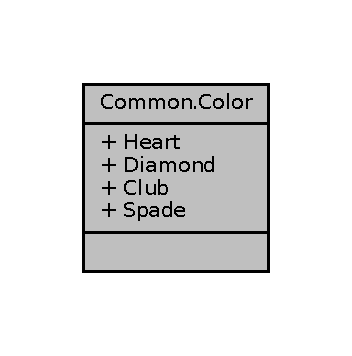
\includegraphics[width=169pt]{enumCommon_1_1Color__coll__graph}
\end{center}
\end{figure}
\subsection*{Public Attributes}
\begin{DoxyCompactItemize}
\item 
\mbox{\hyperlink{enumCommon_1_1Color_aef9e92e2320c284704b9892e75bf8348}{Heart}}
\item 
\mbox{\hyperlink{enumCommon_1_1Color_a381cca0ea5d34bf5485690ec7d062ce4}{Diamond}}
\item 
\mbox{\hyperlink{enumCommon_1_1Color_a42ab11d21245c4e7bb94bd225cb54e13}{Club}}
\item 
\mbox{\hyperlink{enumCommon_1_1Color_a29e2b0d9c5ccdf8a1d449c41ebffc5d7}{Spade}}
\end{DoxyCompactItemize}


\subsection{Member Data Documentation}
\mbox{\Hypertarget{enumCommon_1_1Color_a42ab11d21245c4e7bb94bd225cb54e13}\label{enumCommon_1_1Color_a42ab11d21245c4e7bb94bd225cb54e13}} 
\index{Common\+::\+Color@{Common\+::\+Color}!Club@{Club}}
\index{Club@{Club}!Common\+::\+Color@{Common\+::\+Color}}
\subsubsection{\texorpdfstring{Club}{Club}}
{\footnotesize\ttfamily Common.\+Color.\+Club}

\mbox{\Hypertarget{enumCommon_1_1Color_a381cca0ea5d34bf5485690ec7d062ce4}\label{enumCommon_1_1Color_a381cca0ea5d34bf5485690ec7d062ce4}} 
\index{Common\+::\+Color@{Common\+::\+Color}!Diamond@{Diamond}}
\index{Diamond@{Diamond}!Common\+::\+Color@{Common\+::\+Color}}
\subsubsection{\texorpdfstring{Diamond}{Diamond}}
{\footnotesize\ttfamily Common.\+Color.\+Diamond}

\mbox{\Hypertarget{enumCommon_1_1Color_aef9e92e2320c284704b9892e75bf8348}\label{enumCommon_1_1Color_aef9e92e2320c284704b9892e75bf8348}} 
\index{Common\+::\+Color@{Common\+::\+Color}!Heart@{Heart}}
\index{Heart@{Heart}!Common\+::\+Color@{Common\+::\+Color}}
\subsubsection{\texorpdfstring{Heart}{Heart}}
{\footnotesize\ttfamily Common.\+Color.\+Heart}

\mbox{\Hypertarget{enumCommon_1_1Color_a29e2b0d9c5ccdf8a1d449c41ebffc5d7}\label{enumCommon_1_1Color_a29e2b0d9c5ccdf8a1d449c41ebffc5d7}} 
\index{Common\+::\+Color@{Common\+::\+Color}!Spade@{Spade}}
\index{Spade@{Spade}!Common\+::\+Color@{Common\+::\+Color}}
\subsubsection{\texorpdfstring{Spade}{Spade}}
{\footnotesize\ttfamily Common.\+Color.\+Spade}



The documentation for this enum was generated from the following file\+:\begin{DoxyCompactItemize}
\item 
/home/tetard/\+Idea\+Projects/j\+Coinche/\+Java\+\_\+jcoinche\+\_\+2017/src/main/java/\+Common/\mbox{\hyperlink{Color_8java}{Color.\+java}}\end{DoxyCompactItemize}

\hypertarget{classClient_1_1Controller}{}\section{Client.\+Controller Class Reference}
\label{classClient_1_1Controller}\index{Client.\+Controller@{Client.\+Controller}}


Collaboration diagram for Client.\+Controller\+:
\nopagebreak
\begin{figure}[H]
\begin{center}
\leavevmode
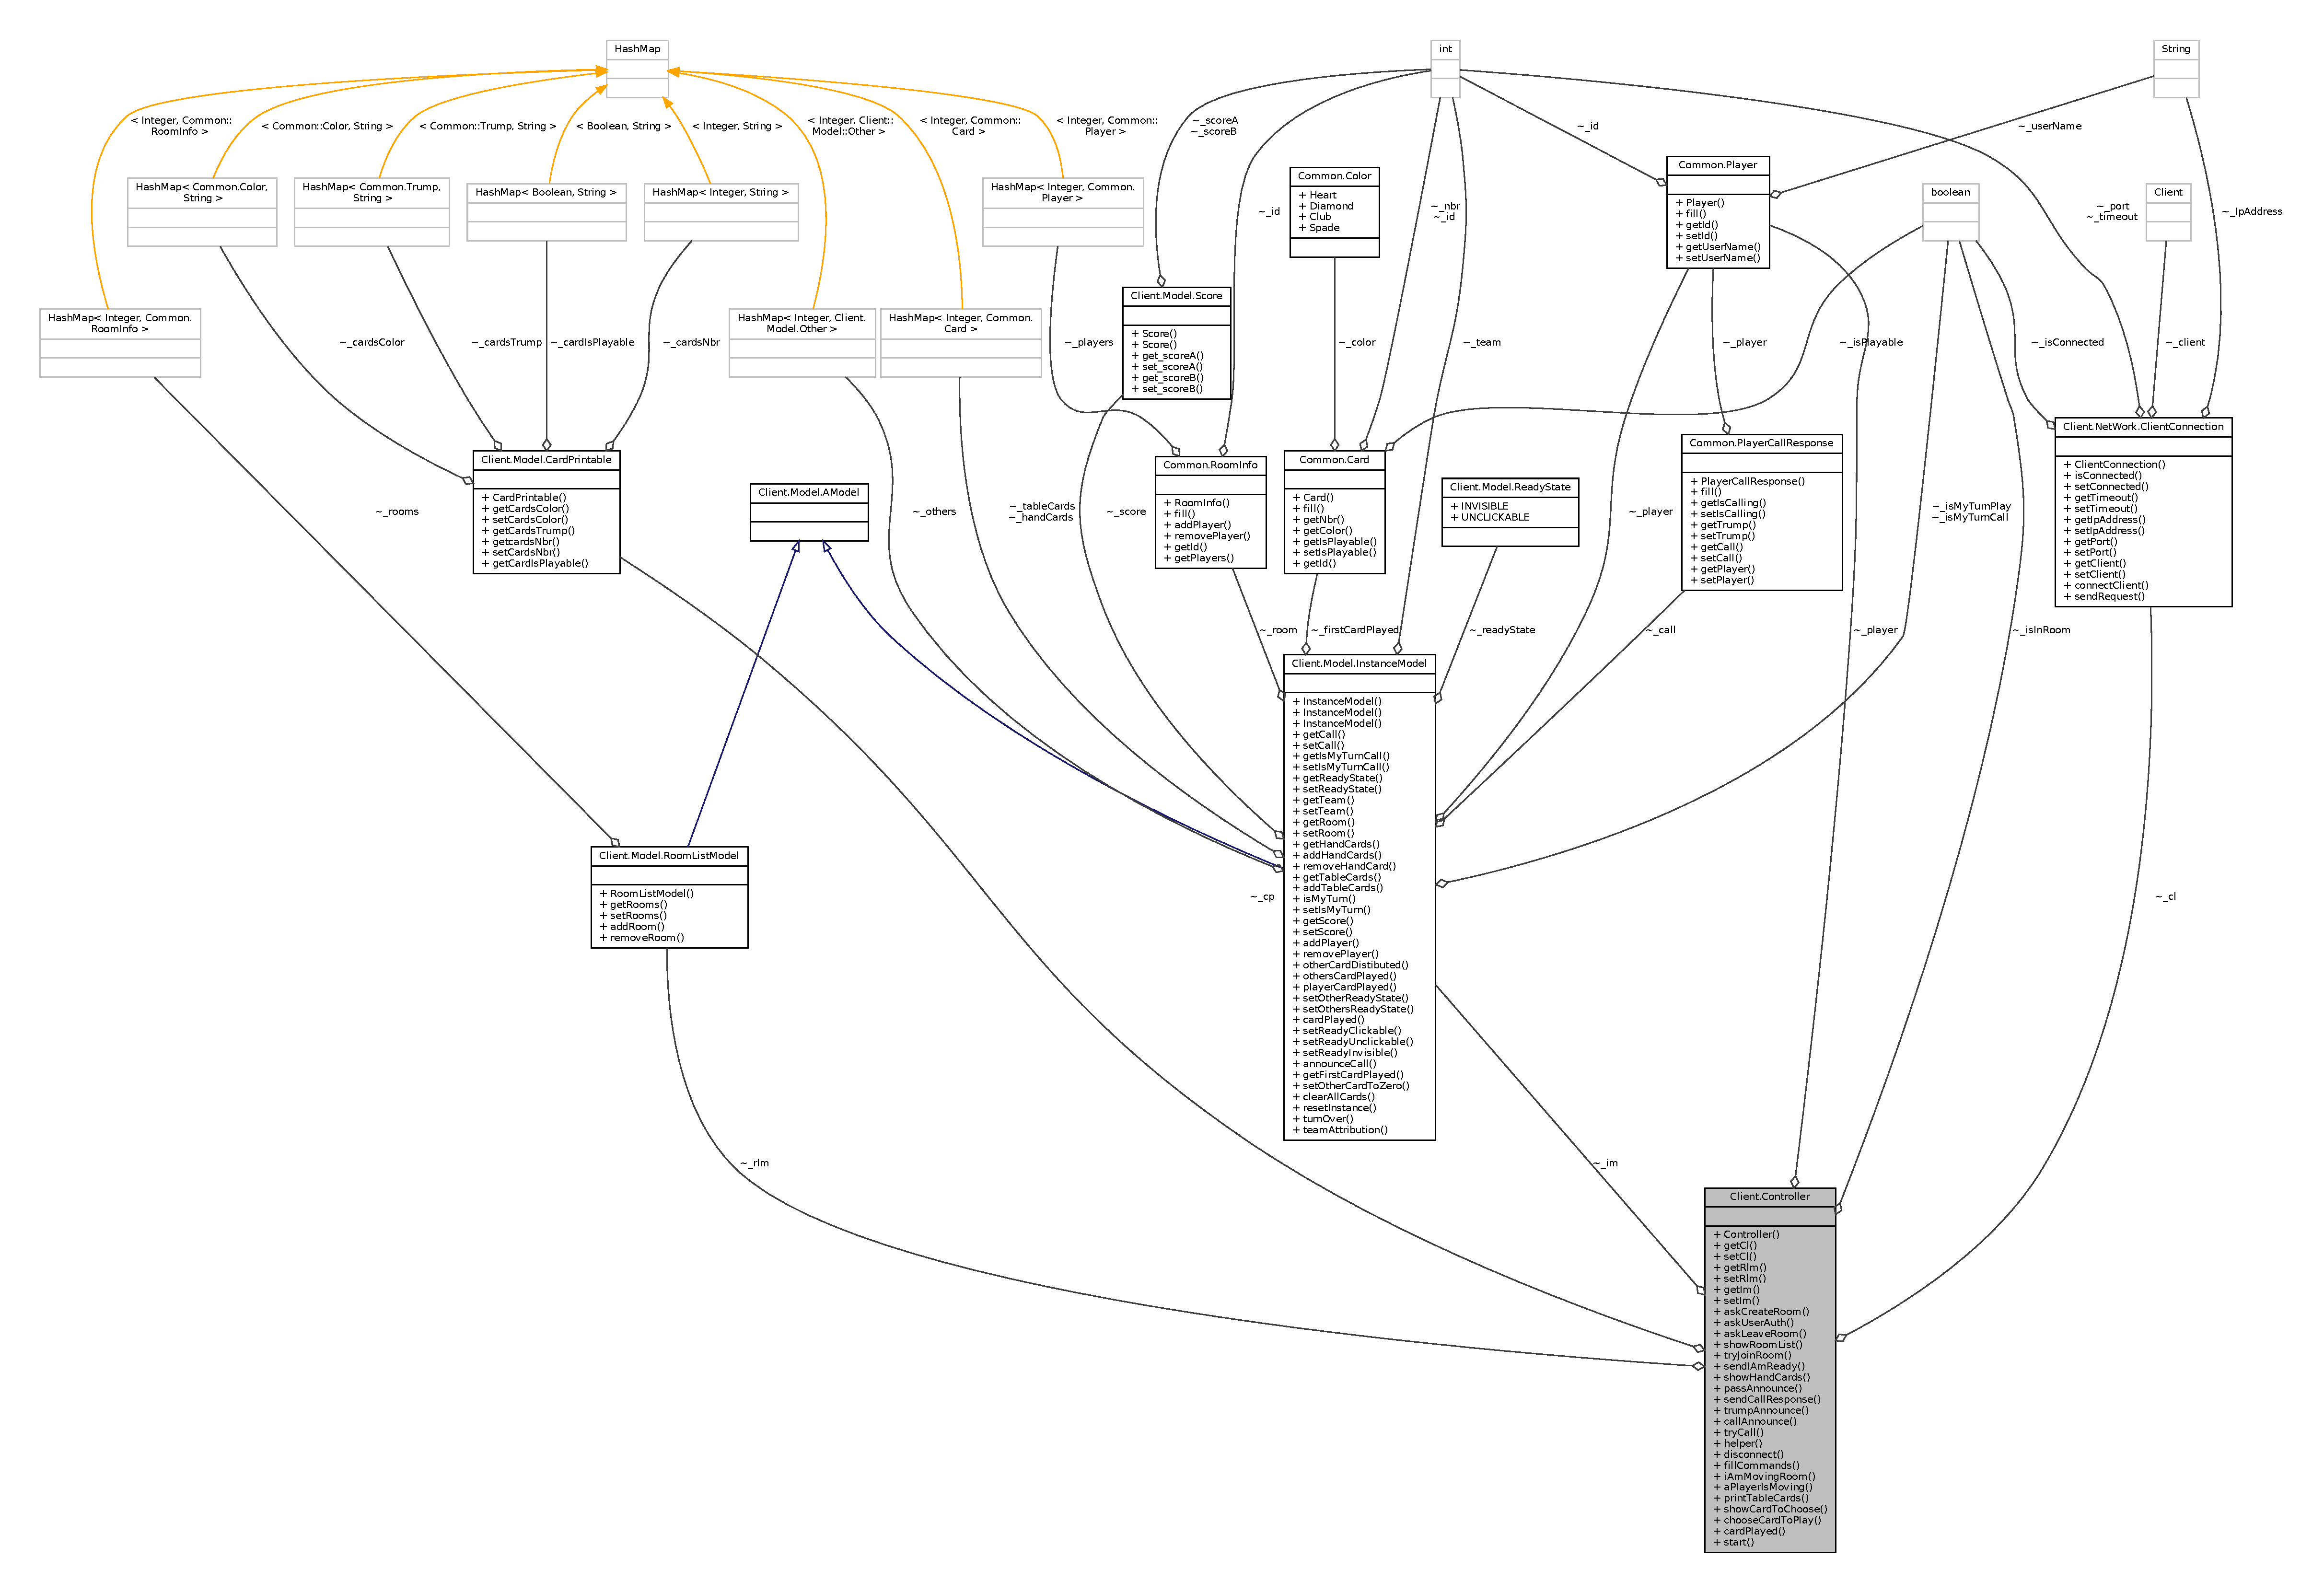
\includegraphics[width=350pt]{classClient_1_1Controller__coll__graph}
\end{center}
\end{figure}
\subsection*{Public Member Functions}
\begin{DoxyCompactItemize}
\item 
\mbox{\hyperlink{classClient_1_1Controller_a65c1ddbad549d42f6ba2f6b3399298f3}{Controller}} (String ip\+Adress, int port)  throws I\+O\+Exception 
\item 
\mbox{\hyperlink{classClient_1_1NetWork_1_1ClientConnection}{Client\+Connection}} \mbox{\hyperlink{classClient_1_1Controller_a4fa5b128b0e5bc44b3d43d43a0138947}{get\+Cl}} ()
\item 
void \mbox{\hyperlink{classClient_1_1Controller_a8ceabaf6a812062b80ac436051788c80}{set\+Cl}} (\mbox{\hyperlink{classClient_1_1NetWork_1_1ClientConnection}{Client\+Connection}} cl)
\item 
\mbox{\hyperlink{classClient_1_1Model_1_1RoomListModel}{Room\+List\+Model}} \mbox{\hyperlink{classClient_1_1Controller_ab33c8837d38c317e03eb6e85e004b586}{get\+Rlm}} ()
\item 
void \mbox{\hyperlink{classClient_1_1Controller_a5d1f7a0a03cf8c3fc186e146ee120ba4}{set\+Rlm}} (\mbox{\hyperlink{classClient_1_1Model_1_1RoomListModel}{Room\+List\+Model}} rlm)
\item 
\mbox{\hyperlink{classClient_1_1Model_1_1InstanceModel}{Instance\+Model}} \mbox{\hyperlink{classClient_1_1Controller_a5cf5f6cb57dab7e260afbf74d6fb4172}{get\+Im}} ()
\item 
void \mbox{\hyperlink{classClient_1_1Controller_a1fc8a5aa222b67716c38d619859f705f}{set\+Im}} (\mbox{\hyperlink{classClient_1_1Model_1_1InstanceModel}{Instance\+Model}} im)
\item 
void \mbox{\hyperlink{classClient_1_1Controller_af3340930e5e87ff85c999d1ace5599e5}{ask\+Create\+Room}} ()
\item 
void \mbox{\hyperlink{classClient_1_1Controller_a4fc90c7e8e74086df88c51eed886c3b8}{ask\+User\+Auth}} ()
\item 
void \mbox{\hyperlink{classClient_1_1Controller_af426bc10eea7f6e7655ff2236b8c160f}{ask\+Leave\+Room}} ()
\item 
void \mbox{\hyperlink{classClient_1_1Controller_a934e1454a2178677cfb7df0d6a6ae54e}{show\+Room\+List}} ()
\item 
void \mbox{\hyperlink{classClient_1_1Controller_af60204a5c842fb77982ae3e8e6635f62}{try\+Join\+Room}} ()
\item 
void \mbox{\hyperlink{classClient_1_1Controller_a7c0ed9c77e04d29b17c75f1141c2bb48}{send\+I\+Am\+Ready}} ()
\item 
void \mbox{\hyperlink{classClient_1_1Controller_a82502998a9b3553fb2ab6430f5b4c423}{show\+Hand\+Cards}} ()
\item 
void \mbox{\hyperlink{classClient_1_1Controller_ad5bc67e5929bedf225177d9df9179bfa}{pass\+Announce}} ()
\item 
void \mbox{\hyperlink{classClient_1_1Controller_a8d3cf754e228f3ca544c718a27f7877c}{send\+Call\+Response}} (\mbox{\hyperlink{enumCommon_1_1Trump}{Trump}} trump, int call)
\item 
void \mbox{\hyperlink{classClient_1_1Controller_af842d2577950491742f5843b6c8c2a93}{trump\+Announce}} (int call)
\item 
void \mbox{\hyperlink{classClient_1_1Controller_a01335f929950989cf1723b1b845cdd6d}{call\+Announce}} ()
\item 
void \mbox{\hyperlink{classClient_1_1Controller_ab188da27fe6cdc563242921dc3028764}{try\+Call}} ()
\item 
void \mbox{\hyperlink{classClient_1_1Controller_af7c67fae279ad06b4513ef68ac71294c}{helper}} ()
\item 
void \mbox{\hyperlink{classClient_1_1Controller_a36f8d304cc2e332a5cab8152dc85d2c0}{disconnect}} ()
\item 
void \mbox{\hyperlink{classClient_1_1Controller_af9f113ff4ab7d8cd478289337df6a423}{fill\+Commands}} (Hash\+Map$<$ String, Runnable $>$ commands)
\item 
void \mbox{\hyperlink{classClient_1_1Controller_a71280e16a0746357f5a7302cfb6a0ac8}{i\+Am\+Moving\+Room}} (\mbox{\hyperlink{classCommon_1_1RoomMovingClient}{Room\+Moving\+Client}} move\+Info, \mbox{\hyperlink{classCommon_1_1RoomInfo}{Room\+Info}} modified\+Room)
\item 
void \mbox{\hyperlink{classClient_1_1Controller_a880e33fad7f0f2ad543ead04bcd6d2b7}{a\+Player\+Is\+Moving}} (\mbox{\hyperlink{classCommon_1_1RoomMovingClient}{Room\+Moving\+Client}} move\+Info, \mbox{\hyperlink{classCommon_1_1RoomInfo}{Room\+Info}} modified\+Room)
\item 
void \mbox{\hyperlink{classClient_1_1Controller_a0998c48fef0c6299b77d130b0e0e55e9}{print\+Table\+Cards}} ()
\item 
void \mbox{\hyperlink{classClient_1_1Controller_a09f717b23bc1405a9376b308797f8bd1}{show\+Card\+To\+Choose}} ()
\item 
void \mbox{\hyperlink{classClient_1_1Controller_ab9335d600e913fdff0adec8b7f2e7e8a}{choose\+Card\+To\+Play}} ()
\item 
void \mbox{\hyperlink{classClient_1_1Controller_a00dd0f9866d799470fa967da62f8964b}{card\+Played}} (\mbox{\hyperlink{classCommon_1_1CardPlayed}{Card\+Played}} card\+Played)
\item 
void \mbox{\hyperlink{classClient_1_1Controller_ae9bd948fb834b86f9b6bee647082bda9}{start}} ()  throws Interrupted\+Exception 
\end{DoxyCompactItemize}


\subsection{Constructor \& Destructor Documentation}
\mbox{\Hypertarget{classClient_1_1Controller_a65c1ddbad549d42f6ba2f6b3399298f3}\label{classClient_1_1Controller_a65c1ddbad549d42f6ba2f6b3399298f3}} 
\index{Client\+::\+Controller@{Client\+::\+Controller}!Controller@{Controller}}
\index{Controller@{Controller}!Client\+::\+Controller@{Client\+::\+Controller}}
\subsubsection{\texorpdfstring{Controller()}{Controller()}}
{\footnotesize\ttfamily Client.\+Controller.\+Controller (\begin{DoxyParamCaption}\item[{String}]{ip\+Adress,  }\item[{int}]{port }\end{DoxyParamCaption}) throws I\+O\+Exception\hspace{0.3cm}{\ttfamily [inline]}}



\subsection{Member Function Documentation}
\mbox{\Hypertarget{classClient_1_1Controller_a880e33fad7f0f2ad543ead04bcd6d2b7}\label{classClient_1_1Controller_a880e33fad7f0f2ad543ead04bcd6d2b7}} 
\index{Client\+::\+Controller@{Client\+::\+Controller}!a\+Player\+Is\+Moving@{a\+Player\+Is\+Moving}}
\index{a\+Player\+Is\+Moving@{a\+Player\+Is\+Moving}!Client\+::\+Controller@{Client\+::\+Controller}}
\subsubsection{\texorpdfstring{a\+Player\+Is\+Moving()}{aPlayerIsMoving()}}
{\footnotesize\ttfamily void Client.\+Controller.\+a\+Player\+Is\+Moving (\begin{DoxyParamCaption}\item[{\mbox{\hyperlink{classCommon_1_1RoomMovingClient}{Room\+Moving\+Client}}}]{move\+Info,  }\item[{\mbox{\hyperlink{classCommon_1_1RoomInfo}{Room\+Info}}}]{modified\+Room }\end{DoxyParamCaption})\hspace{0.3cm}{\ttfamily [inline]}}

\mbox{\Hypertarget{classClient_1_1Controller_af3340930e5e87ff85c999d1ace5599e5}\label{classClient_1_1Controller_af3340930e5e87ff85c999d1ace5599e5}} 
\index{Client\+::\+Controller@{Client\+::\+Controller}!ask\+Create\+Room@{ask\+Create\+Room}}
\index{ask\+Create\+Room@{ask\+Create\+Room}!Client\+::\+Controller@{Client\+::\+Controller}}
\subsubsection{\texorpdfstring{ask\+Create\+Room()}{askCreateRoom()}}
{\footnotesize\ttfamily void Client.\+Controller.\+ask\+Create\+Room (\begin{DoxyParamCaption}{ }\end{DoxyParamCaption})\hspace{0.3cm}{\ttfamily [inline]}}

\mbox{\Hypertarget{classClient_1_1Controller_af426bc10eea7f6e7655ff2236b8c160f}\label{classClient_1_1Controller_af426bc10eea7f6e7655ff2236b8c160f}} 
\index{Client\+::\+Controller@{Client\+::\+Controller}!ask\+Leave\+Room@{ask\+Leave\+Room}}
\index{ask\+Leave\+Room@{ask\+Leave\+Room}!Client\+::\+Controller@{Client\+::\+Controller}}
\subsubsection{\texorpdfstring{ask\+Leave\+Room()}{askLeaveRoom()}}
{\footnotesize\ttfamily void Client.\+Controller.\+ask\+Leave\+Room (\begin{DoxyParamCaption}{ }\end{DoxyParamCaption})\hspace{0.3cm}{\ttfamily [inline]}}

\mbox{\Hypertarget{classClient_1_1Controller_a4fc90c7e8e74086df88c51eed886c3b8}\label{classClient_1_1Controller_a4fc90c7e8e74086df88c51eed886c3b8}} 
\index{Client\+::\+Controller@{Client\+::\+Controller}!ask\+User\+Auth@{ask\+User\+Auth}}
\index{ask\+User\+Auth@{ask\+User\+Auth}!Client\+::\+Controller@{Client\+::\+Controller}}
\subsubsection{\texorpdfstring{ask\+User\+Auth()}{askUserAuth()}}
{\footnotesize\ttfamily void Client.\+Controller.\+ask\+User\+Auth (\begin{DoxyParamCaption}{ }\end{DoxyParamCaption})\hspace{0.3cm}{\ttfamily [inline]}}

\mbox{\Hypertarget{classClient_1_1Controller_a01335f929950989cf1723b1b845cdd6d}\label{classClient_1_1Controller_a01335f929950989cf1723b1b845cdd6d}} 
\index{Client\+::\+Controller@{Client\+::\+Controller}!call\+Announce@{call\+Announce}}
\index{call\+Announce@{call\+Announce}!Client\+::\+Controller@{Client\+::\+Controller}}
\subsubsection{\texorpdfstring{call\+Announce()}{callAnnounce()}}
{\footnotesize\ttfamily void Client.\+Controller.\+call\+Announce (\begin{DoxyParamCaption}{ }\end{DoxyParamCaption})\hspace{0.3cm}{\ttfamily [inline]}}

\mbox{\Hypertarget{classClient_1_1Controller_a00dd0f9866d799470fa967da62f8964b}\label{classClient_1_1Controller_a00dd0f9866d799470fa967da62f8964b}} 
\index{Client\+::\+Controller@{Client\+::\+Controller}!card\+Played@{card\+Played}}
\index{card\+Played@{card\+Played}!Client\+::\+Controller@{Client\+::\+Controller}}
\subsubsection{\texorpdfstring{card\+Played()}{cardPlayed()}}
{\footnotesize\ttfamily void Client.\+Controller.\+card\+Played (\begin{DoxyParamCaption}\item[{\mbox{\hyperlink{classCommon_1_1CardPlayed}{Card\+Played}}}]{card\+Played }\end{DoxyParamCaption})\hspace{0.3cm}{\ttfamily [inline]}}

\mbox{\Hypertarget{classClient_1_1Controller_ab9335d600e913fdff0adec8b7f2e7e8a}\label{classClient_1_1Controller_ab9335d600e913fdff0adec8b7f2e7e8a}} 
\index{Client\+::\+Controller@{Client\+::\+Controller}!choose\+Card\+To\+Play@{choose\+Card\+To\+Play}}
\index{choose\+Card\+To\+Play@{choose\+Card\+To\+Play}!Client\+::\+Controller@{Client\+::\+Controller}}
\subsubsection{\texorpdfstring{choose\+Card\+To\+Play()}{chooseCardToPlay()}}
{\footnotesize\ttfamily void Client.\+Controller.\+choose\+Card\+To\+Play (\begin{DoxyParamCaption}{ }\end{DoxyParamCaption})\hspace{0.3cm}{\ttfamily [inline]}}

\mbox{\Hypertarget{classClient_1_1Controller_a36f8d304cc2e332a5cab8152dc85d2c0}\label{classClient_1_1Controller_a36f8d304cc2e332a5cab8152dc85d2c0}} 
\index{Client\+::\+Controller@{Client\+::\+Controller}!disconnect@{disconnect}}
\index{disconnect@{disconnect}!Client\+::\+Controller@{Client\+::\+Controller}}
\subsubsection{\texorpdfstring{disconnect()}{disconnect()}}
{\footnotesize\ttfamily void Client.\+Controller.\+disconnect (\begin{DoxyParamCaption}{ }\end{DoxyParamCaption})\hspace{0.3cm}{\ttfamily [inline]}}

\mbox{\Hypertarget{classClient_1_1Controller_af9f113ff4ab7d8cd478289337df6a423}\label{classClient_1_1Controller_af9f113ff4ab7d8cd478289337df6a423}} 
\index{Client\+::\+Controller@{Client\+::\+Controller}!fill\+Commands@{fill\+Commands}}
\index{fill\+Commands@{fill\+Commands}!Client\+::\+Controller@{Client\+::\+Controller}}
\subsubsection{\texorpdfstring{fill\+Commands()}{fillCommands()}}
{\footnotesize\ttfamily void Client.\+Controller.\+fill\+Commands (\begin{DoxyParamCaption}\item[{Hash\+Map$<$ String, Runnable $>$}]{commands }\end{DoxyParamCaption})\hspace{0.3cm}{\ttfamily [inline]}}

\mbox{\Hypertarget{classClient_1_1Controller_a4fa5b128b0e5bc44b3d43d43a0138947}\label{classClient_1_1Controller_a4fa5b128b0e5bc44b3d43d43a0138947}} 
\index{Client\+::\+Controller@{Client\+::\+Controller}!get\+Cl@{get\+Cl}}
\index{get\+Cl@{get\+Cl}!Client\+::\+Controller@{Client\+::\+Controller}}
\subsubsection{\texorpdfstring{get\+Cl()}{getCl()}}
{\footnotesize\ttfamily \mbox{\hyperlink{classClient_1_1NetWork_1_1ClientConnection}{Client\+Connection}} Client.\+Controller.\+get\+Cl (\begin{DoxyParamCaption}{ }\end{DoxyParamCaption})\hspace{0.3cm}{\ttfamily [inline]}}

\mbox{\Hypertarget{classClient_1_1Controller_a5cf5f6cb57dab7e260afbf74d6fb4172}\label{classClient_1_1Controller_a5cf5f6cb57dab7e260afbf74d6fb4172}} 
\index{Client\+::\+Controller@{Client\+::\+Controller}!get\+Im@{get\+Im}}
\index{get\+Im@{get\+Im}!Client\+::\+Controller@{Client\+::\+Controller}}
\subsubsection{\texorpdfstring{get\+Im()}{getIm()}}
{\footnotesize\ttfamily \mbox{\hyperlink{classClient_1_1Model_1_1InstanceModel}{Instance\+Model}} Client.\+Controller.\+get\+Im (\begin{DoxyParamCaption}{ }\end{DoxyParamCaption})\hspace{0.3cm}{\ttfamily [inline]}}

\mbox{\Hypertarget{classClient_1_1Controller_ab33c8837d38c317e03eb6e85e004b586}\label{classClient_1_1Controller_ab33c8837d38c317e03eb6e85e004b586}} 
\index{Client\+::\+Controller@{Client\+::\+Controller}!get\+Rlm@{get\+Rlm}}
\index{get\+Rlm@{get\+Rlm}!Client\+::\+Controller@{Client\+::\+Controller}}
\subsubsection{\texorpdfstring{get\+Rlm()}{getRlm()}}
{\footnotesize\ttfamily \mbox{\hyperlink{classClient_1_1Model_1_1RoomListModel}{Room\+List\+Model}} Client.\+Controller.\+get\+Rlm (\begin{DoxyParamCaption}{ }\end{DoxyParamCaption})\hspace{0.3cm}{\ttfamily [inline]}}

\mbox{\Hypertarget{classClient_1_1Controller_af7c67fae279ad06b4513ef68ac71294c}\label{classClient_1_1Controller_af7c67fae279ad06b4513ef68ac71294c}} 
\index{Client\+::\+Controller@{Client\+::\+Controller}!helper@{helper}}
\index{helper@{helper}!Client\+::\+Controller@{Client\+::\+Controller}}
\subsubsection{\texorpdfstring{helper()}{helper()}}
{\footnotesize\ttfamily void Client.\+Controller.\+helper (\begin{DoxyParamCaption}{ }\end{DoxyParamCaption})\hspace{0.3cm}{\ttfamily [inline]}}

\mbox{\Hypertarget{classClient_1_1Controller_a71280e16a0746357f5a7302cfb6a0ac8}\label{classClient_1_1Controller_a71280e16a0746357f5a7302cfb6a0ac8}} 
\index{Client\+::\+Controller@{Client\+::\+Controller}!i\+Am\+Moving\+Room@{i\+Am\+Moving\+Room}}
\index{i\+Am\+Moving\+Room@{i\+Am\+Moving\+Room}!Client\+::\+Controller@{Client\+::\+Controller}}
\subsubsection{\texorpdfstring{i\+Am\+Moving\+Room()}{iAmMovingRoom()}}
{\footnotesize\ttfamily void Client.\+Controller.\+i\+Am\+Moving\+Room (\begin{DoxyParamCaption}\item[{\mbox{\hyperlink{classCommon_1_1RoomMovingClient}{Room\+Moving\+Client}}}]{move\+Info,  }\item[{\mbox{\hyperlink{classCommon_1_1RoomInfo}{Room\+Info}}}]{modified\+Room }\end{DoxyParamCaption})\hspace{0.3cm}{\ttfamily [inline]}}

\mbox{\Hypertarget{classClient_1_1Controller_ad5bc67e5929bedf225177d9df9179bfa}\label{classClient_1_1Controller_ad5bc67e5929bedf225177d9df9179bfa}} 
\index{Client\+::\+Controller@{Client\+::\+Controller}!pass\+Announce@{pass\+Announce}}
\index{pass\+Announce@{pass\+Announce}!Client\+::\+Controller@{Client\+::\+Controller}}
\subsubsection{\texorpdfstring{pass\+Announce()}{passAnnounce()}}
{\footnotesize\ttfamily void Client.\+Controller.\+pass\+Announce (\begin{DoxyParamCaption}{ }\end{DoxyParamCaption})\hspace{0.3cm}{\ttfamily [inline]}}

\mbox{\Hypertarget{classClient_1_1Controller_a0998c48fef0c6299b77d130b0e0e55e9}\label{classClient_1_1Controller_a0998c48fef0c6299b77d130b0e0e55e9}} 
\index{Client\+::\+Controller@{Client\+::\+Controller}!print\+Table\+Cards@{print\+Table\+Cards}}
\index{print\+Table\+Cards@{print\+Table\+Cards}!Client\+::\+Controller@{Client\+::\+Controller}}
\subsubsection{\texorpdfstring{print\+Table\+Cards()}{printTableCards()}}
{\footnotesize\ttfamily void Client.\+Controller.\+print\+Table\+Cards (\begin{DoxyParamCaption}{ }\end{DoxyParamCaption})\hspace{0.3cm}{\ttfamily [inline]}}

\mbox{\Hypertarget{classClient_1_1Controller_a8d3cf754e228f3ca544c718a27f7877c}\label{classClient_1_1Controller_a8d3cf754e228f3ca544c718a27f7877c}} 
\index{Client\+::\+Controller@{Client\+::\+Controller}!send\+Call\+Response@{send\+Call\+Response}}
\index{send\+Call\+Response@{send\+Call\+Response}!Client\+::\+Controller@{Client\+::\+Controller}}
\subsubsection{\texorpdfstring{send\+Call\+Response()}{sendCallResponse()}}
{\footnotesize\ttfamily void Client.\+Controller.\+send\+Call\+Response (\begin{DoxyParamCaption}\item[{\mbox{\hyperlink{enumCommon_1_1Trump}{Trump}}}]{trump,  }\item[{int}]{call }\end{DoxyParamCaption})\hspace{0.3cm}{\ttfamily [inline]}}

\mbox{\Hypertarget{classClient_1_1Controller_a7c0ed9c77e04d29b17c75f1141c2bb48}\label{classClient_1_1Controller_a7c0ed9c77e04d29b17c75f1141c2bb48}} 
\index{Client\+::\+Controller@{Client\+::\+Controller}!send\+I\+Am\+Ready@{send\+I\+Am\+Ready}}
\index{send\+I\+Am\+Ready@{send\+I\+Am\+Ready}!Client\+::\+Controller@{Client\+::\+Controller}}
\subsubsection{\texorpdfstring{send\+I\+Am\+Ready()}{sendIAmReady()}}
{\footnotesize\ttfamily void Client.\+Controller.\+send\+I\+Am\+Ready (\begin{DoxyParamCaption}{ }\end{DoxyParamCaption})\hspace{0.3cm}{\ttfamily [inline]}}

\mbox{\Hypertarget{classClient_1_1Controller_a8ceabaf6a812062b80ac436051788c80}\label{classClient_1_1Controller_a8ceabaf6a812062b80ac436051788c80}} 
\index{Client\+::\+Controller@{Client\+::\+Controller}!set\+Cl@{set\+Cl}}
\index{set\+Cl@{set\+Cl}!Client\+::\+Controller@{Client\+::\+Controller}}
\subsubsection{\texorpdfstring{set\+Cl()}{setCl()}}
{\footnotesize\ttfamily void Client.\+Controller.\+set\+Cl (\begin{DoxyParamCaption}\item[{\mbox{\hyperlink{classClient_1_1NetWork_1_1ClientConnection}{Client\+Connection}}}]{cl }\end{DoxyParamCaption})\hspace{0.3cm}{\ttfamily [inline]}}

\mbox{\Hypertarget{classClient_1_1Controller_a1fc8a5aa222b67716c38d619859f705f}\label{classClient_1_1Controller_a1fc8a5aa222b67716c38d619859f705f}} 
\index{Client\+::\+Controller@{Client\+::\+Controller}!set\+Im@{set\+Im}}
\index{set\+Im@{set\+Im}!Client\+::\+Controller@{Client\+::\+Controller}}
\subsubsection{\texorpdfstring{set\+Im()}{setIm()}}
{\footnotesize\ttfamily void Client.\+Controller.\+set\+Im (\begin{DoxyParamCaption}\item[{\mbox{\hyperlink{classClient_1_1Model_1_1InstanceModel}{Instance\+Model}}}]{im }\end{DoxyParamCaption})\hspace{0.3cm}{\ttfamily [inline]}}

\mbox{\Hypertarget{classClient_1_1Controller_a5d1f7a0a03cf8c3fc186e146ee120ba4}\label{classClient_1_1Controller_a5d1f7a0a03cf8c3fc186e146ee120ba4}} 
\index{Client\+::\+Controller@{Client\+::\+Controller}!set\+Rlm@{set\+Rlm}}
\index{set\+Rlm@{set\+Rlm}!Client\+::\+Controller@{Client\+::\+Controller}}
\subsubsection{\texorpdfstring{set\+Rlm()}{setRlm()}}
{\footnotesize\ttfamily void Client.\+Controller.\+set\+Rlm (\begin{DoxyParamCaption}\item[{\mbox{\hyperlink{classClient_1_1Model_1_1RoomListModel}{Room\+List\+Model}}}]{rlm }\end{DoxyParamCaption})\hspace{0.3cm}{\ttfamily [inline]}}

\mbox{\Hypertarget{classClient_1_1Controller_a09f717b23bc1405a9376b308797f8bd1}\label{classClient_1_1Controller_a09f717b23bc1405a9376b308797f8bd1}} 
\index{Client\+::\+Controller@{Client\+::\+Controller}!show\+Card\+To\+Choose@{show\+Card\+To\+Choose}}
\index{show\+Card\+To\+Choose@{show\+Card\+To\+Choose}!Client\+::\+Controller@{Client\+::\+Controller}}
\subsubsection{\texorpdfstring{show\+Card\+To\+Choose()}{showCardToChoose()}}
{\footnotesize\ttfamily void Client.\+Controller.\+show\+Card\+To\+Choose (\begin{DoxyParamCaption}{ }\end{DoxyParamCaption})\hspace{0.3cm}{\ttfamily [inline]}}

\mbox{\Hypertarget{classClient_1_1Controller_a82502998a9b3553fb2ab6430f5b4c423}\label{classClient_1_1Controller_a82502998a9b3553fb2ab6430f5b4c423}} 
\index{Client\+::\+Controller@{Client\+::\+Controller}!show\+Hand\+Cards@{show\+Hand\+Cards}}
\index{show\+Hand\+Cards@{show\+Hand\+Cards}!Client\+::\+Controller@{Client\+::\+Controller}}
\subsubsection{\texorpdfstring{show\+Hand\+Cards()}{showHandCards()}}
{\footnotesize\ttfamily void Client.\+Controller.\+show\+Hand\+Cards (\begin{DoxyParamCaption}{ }\end{DoxyParamCaption})\hspace{0.3cm}{\ttfamily [inline]}}

\mbox{\Hypertarget{classClient_1_1Controller_a934e1454a2178677cfb7df0d6a6ae54e}\label{classClient_1_1Controller_a934e1454a2178677cfb7df0d6a6ae54e}} 
\index{Client\+::\+Controller@{Client\+::\+Controller}!show\+Room\+List@{show\+Room\+List}}
\index{show\+Room\+List@{show\+Room\+List}!Client\+::\+Controller@{Client\+::\+Controller}}
\subsubsection{\texorpdfstring{show\+Room\+List()}{showRoomList()}}
{\footnotesize\ttfamily void Client.\+Controller.\+show\+Room\+List (\begin{DoxyParamCaption}{ }\end{DoxyParamCaption})\hspace{0.3cm}{\ttfamily [inline]}}

\mbox{\Hypertarget{classClient_1_1Controller_ae9bd948fb834b86f9b6bee647082bda9}\label{classClient_1_1Controller_ae9bd948fb834b86f9b6bee647082bda9}} 
\index{Client\+::\+Controller@{Client\+::\+Controller}!start@{start}}
\index{start@{start}!Client\+::\+Controller@{Client\+::\+Controller}}
\subsubsection{\texorpdfstring{start()}{start()}}
{\footnotesize\ttfamily void Client.\+Controller.\+start (\begin{DoxyParamCaption}{ }\end{DoxyParamCaption}) throws Interrupted\+Exception\hspace{0.3cm}{\ttfamily [inline]}}

\mbox{\Hypertarget{classClient_1_1Controller_af842d2577950491742f5843b6c8c2a93}\label{classClient_1_1Controller_af842d2577950491742f5843b6c8c2a93}} 
\index{Client\+::\+Controller@{Client\+::\+Controller}!trump\+Announce@{trump\+Announce}}
\index{trump\+Announce@{trump\+Announce}!Client\+::\+Controller@{Client\+::\+Controller}}
\subsubsection{\texorpdfstring{trump\+Announce()}{trumpAnnounce()}}
{\footnotesize\ttfamily void Client.\+Controller.\+trump\+Announce (\begin{DoxyParamCaption}\item[{int}]{call }\end{DoxyParamCaption})\hspace{0.3cm}{\ttfamily [inline]}}

\mbox{\Hypertarget{classClient_1_1Controller_ab188da27fe6cdc563242921dc3028764}\label{classClient_1_1Controller_ab188da27fe6cdc563242921dc3028764}} 
\index{Client\+::\+Controller@{Client\+::\+Controller}!try\+Call@{try\+Call}}
\index{try\+Call@{try\+Call}!Client\+::\+Controller@{Client\+::\+Controller}}
\subsubsection{\texorpdfstring{try\+Call()}{tryCall()}}
{\footnotesize\ttfamily void Client.\+Controller.\+try\+Call (\begin{DoxyParamCaption}{ }\end{DoxyParamCaption})\hspace{0.3cm}{\ttfamily [inline]}}

\mbox{\Hypertarget{classClient_1_1Controller_af60204a5c842fb77982ae3e8e6635f62}\label{classClient_1_1Controller_af60204a5c842fb77982ae3e8e6635f62}} 
\index{Client\+::\+Controller@{Client\+::\+Controller}!try\+Join\+Room@{try\+Join\+Room}}
\index{try\+Join\+Room@{try\+Join\+Room}!Client\+::\+Controller@{Client\+::\+Controller}}
\subsubsection{\texorpdfstring{try\+Join\+Room()}{tryJoinRoom()}}
{\footnotesize\ttfamily void Client.\+Controller.\+try\+Join\+Room (\begin{DoxyParamCaption}{ }\end{DoxyParamCaption})\hspace{0.3cm}{\ttfamily [inline]}}



The documentation for this class was generated from the following file\+:\begin{DoxyCompactItemize}
\item 
/home/tetard/\+Idea\+Projects/j\+Coinche/\+Java\+\_\+jcoinche\+\_\+2017/src/main/java/\+Client/\mbox{\hyperlink{Controller_8java}{Controller.\+java}}\end{DoxyCompactItemize}

\hypertarget{classServer_1_1Core}{}\section{Server.\+Core Class Reference}
\label{classServer_1_1Core}\index{Server.\+Core@{Server.\+Core}}


Collaboration diagram for Server.\+Core\+:
\nopagebreak
\begin{figure}[H]
\begin{center}
\leavevmode
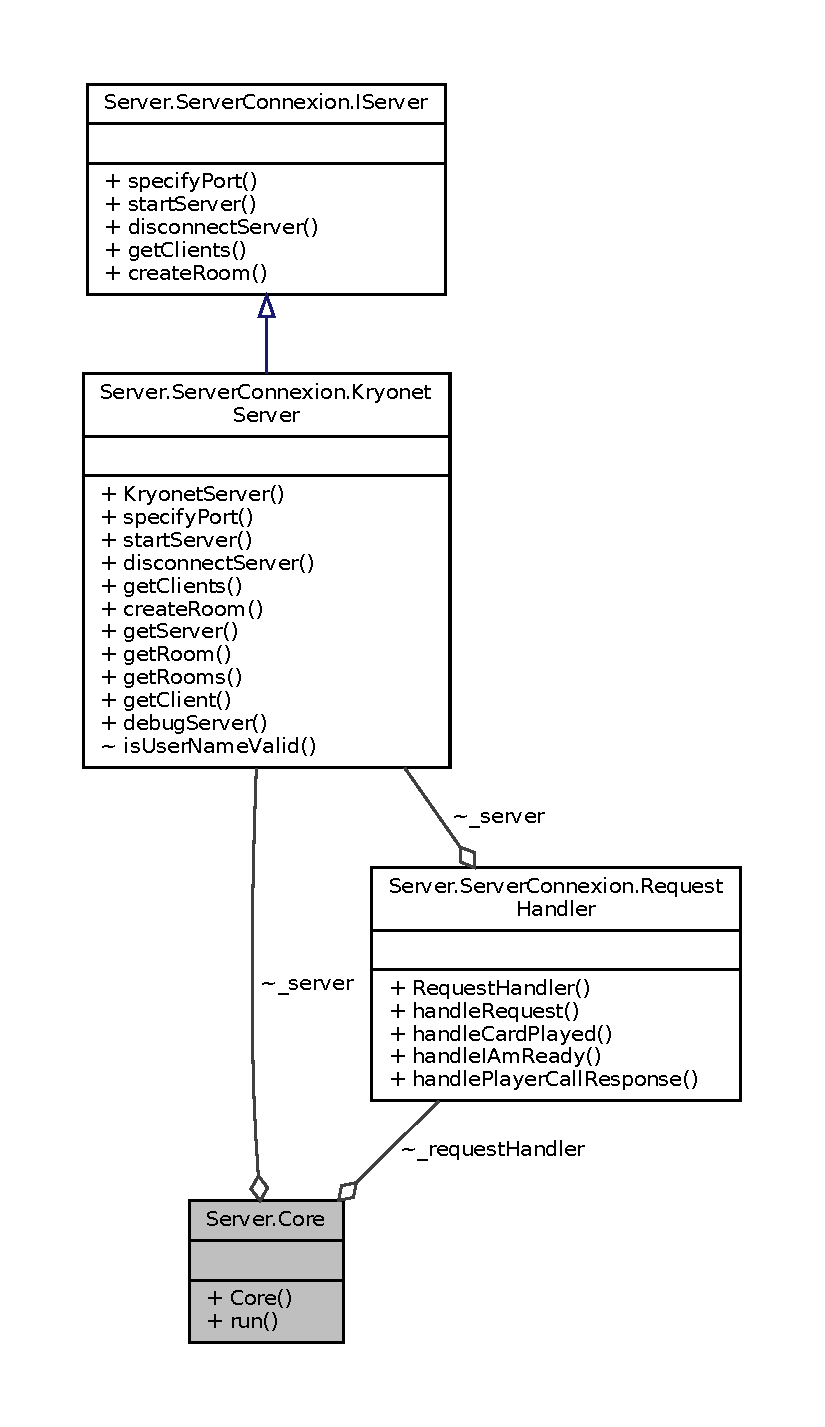
\includegraphics[height=550pt]{classServer_1_1Core__coll__graph}
\end{center}
\end{figure}
\subsection*{Public Member Functions}
\begin{DoxyCompactItemize}
\item 
\mbox{\hyperlink{classServer_1_1Core_a84686707df17f13d058e714bfb4ea47c}{Core}} (int port)
\item 
void \mbox{\hyperlink{classServer_1_1Core_aee36e713f04f6094446647d47edf2765}{run}} ()  throws Interrupted\+Exception, I\+O\+Exception 
\end{DoxyCompactItemize}


\subsection{Constructor \& Destructor Documentation}
\mbox{\Hypertarget{classServer_1_1Core_a84686707df17f13d058e714bfb4ea47c}\label{classServer_1_1Core_a84686707df17f13d058e714bfb4ea47c}} 
\index{Server\+::\+Core@{Server\+::\+Core}!Core@{Core}}
\index{Core@{Core}!Server\+::\+Core@{Server\+::\+Core}}
\subsubsection{\texorpdfstring{Core()}{Core()}}
{\footnotesize\ttfamily Server.\+Core.\+Core (\begin{DoxyParamCaption}\item[{int}]{port }\end{DoxyParamCaption})\hspace{0.3cm}{\ttfamily [inline]}}



\subsection{Member Function Documentation}
\mbox{\Hypertarget{classServer_1_1Core_aee36e713f04f6094446647d47edf2765}\label{classServer_1_1Core_aee36e713f04f6094446647d47edf2765}} 
\index{Server\+::\+Core@{Server\+::\+Core}!run@{run}}
\index{run@{run}!Server\+::\+Core@{Server\+::\+Core}}
\subsubsection{\texorpdfstring{run()}{run()}}
{\footnotesize\ttfamily void Server.\+Core.\+run (\begin{DoxyParamCaption}{ }\end{DoxyParamCaption}) throws Interrupted\+Exception, I\+O\+Exception\hspace{0.3cm}{\ttfamily [inline]}}



The documentation for this class was generated from the following file\+:\begin{DoxyCompactItemize}
\item 
/home/tetard/\+Idea\+Projects/j\+Coinche/\+Java\+\_\+jcoinche\+\_\+2017/src/main/java/\+Server/\mbox{\hyperlink{Core_8java}{Core.\+java}}\end{DoxyCompactItemize}

\hypertarget{classCommon_1_1GameCancelled}{}\section{Common.\+Game\+Cancelled Class Reference}
\label{classCommon_1_1GameCancelled}\index{Common.\+Game\+Cancelled@{Common.\+Game\+Cancelled}}


Collaboration diagram for Common.\+Game\+Cancelled\+:
\nopagebreak
\begin{figure}[H]
\begin{center}
\leavevmode
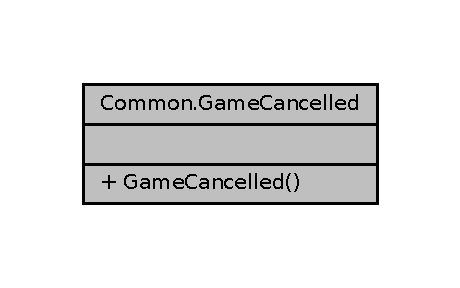
\includegraphics[width=221pt]{classCommon_1_1GameCancelled__coll__graph}
\end{center}
\end{figure}
\subsection*{Public Member Functions}
\begin{DoxyCompactItemize}
\item 
\mbox{\hyperlink{classCommon_1_1GameCancelled_a893afa4f7dbd2469db0042c1043ab3b9}{Game\+Cancelled}} ()
\end{DoxyCompactItemize}


\subsection{Constructor \& Destructor Documentation}
\mbox{\Hypertarget{classCommon_1_1GameCancelled_a893afa4f7dbd2469db0042c1043ab3b9}\label{classCommon_1_1GameCancelled_a893afa4f7dbd2469db0042c1043ab3b9}} 
\index{Common\+::\+Game\+Cancelled@{Common\+::\+Game\+Cancelled}!Game\+Cancelled@{Game\+Cancelled}}
\index{Game\+Cancelled@{Game\+Cancelled}!Common\+::\+Game\+Cancelled@{Common\+::\+Game\+Cancelled}}
\subsubsection{\texorpdfstring{Game\+Cancelled()}{GameCancelled()}}
{\footnotesize\ttfamily Common.\+Game\+Cancelled.\+Game\+Cancelled (\begin{DoxyParamCaption}{ }\end{DoxyParamCaption})\hspace{0.3cm}{\ttfamily [inline]}}



The documentation for this class was generated from the following file\+:\begin{DoxyCompactItemize}
\item 
/home/tetard/\+Idea\+Projects/j\+Coinche/\+Java\+\_\+jcoinche\+\_\+2017/src/main/java/\+Common/\mbox{\hyperlink{GameCancelled_8java}{Game\+Cancelled.\+java}}\end{DoxyCompactItemize}

\hypertarget{classServer_1_1Game_1_1GameInfos}{}\section{Server.\+Game.\+Game\+Infos Class Reference}
\label{classServer_1_1Game_1_1GameInfos}\index{Server.\+Game.\+Game\+Infos@{Server.\+Game.\+Game\+Infos}}


Collaboration diagram for Server.\+Game.\+Game\+Infos\+:
\nopagebreak
\begin{figure}[H]
\begin{center}
\leavevmode
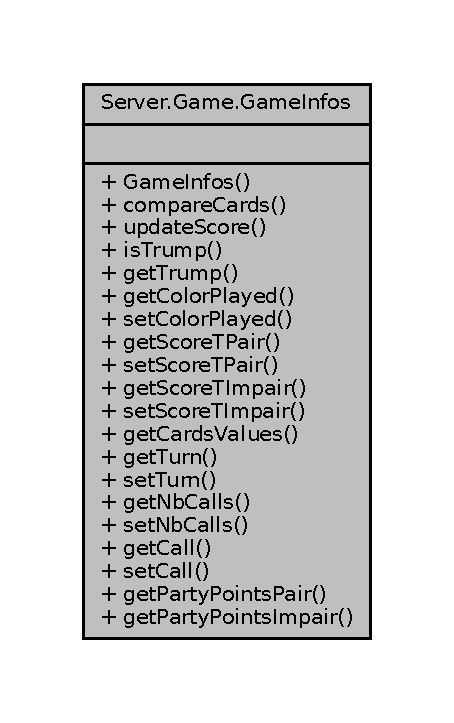
\includegraphics[width=218pt]{classServer_1_1Game_1_1GameInfos__coll__graph}
\end{center}
\end{figure}
\subsection*{Public Member Functions}
\begin{DoxyCompactItemize}
\item 
\mbox{\hyperlink{classServer_1_1Game_1_1GameInfos_a548b3ab8fe42f46062df51f915583b2f}{Game\+Infos}} ()
\item 
boolean \mbox{\hyperlink{classServer_1_1Game_1_1GameInfos_afdd2e6dddeba900ee192cd8f6f3442e0}{compare\+Cards}} (\mbox{\hyperlink{classCommon_1_1Card}{Card}} true\+Card, \mbox{\hyperlink{classCommon_1_1Card}{Card}} false\+Card)
\item 
\mbox{\hyperlink{classServer_1_1ServerConnexion_1_1ClientInfos}{Client\+Infos}} \mbox{\hyperlink{classServer_1_1Game_1_1GameInfos_a29835c070042dbf7eaea067e6c9acbf4}{update\+Score}} (Hash\+Map$<$ \mbox{\hyperlink{classServer_1_1ServerConnexion_1_1ClientInfos}{Client\+Infos}}, \mbox{\hyperlink{classCommon_1_1Card}{Card}} $>$ table\+Cards)
\item 
boolean \mbox{\hyperlink{classServer_1_1Game_1_1GameInfos_a7375e63b9b1bb2da69ca50884030ab46}{is\+Trump}} (\mbox{\hyperlink{classCommon_1_1Card}{Card}} card)
\item 
\mbox{\hyperlink{enumCommon_1_1Trump}{Trump}} \mbox{\hyperlink{classServer_1_1Game_1_1GameInfos_a973c5cddda8e6361dd5910a62bb8fe6e}{get\+Trump}} ()
\item 
\mbox{\hyperlink{enumCommon_1_1Color}{Color}} \mbox{\hyperlink{classServer_1_1Game_1_1GameInfos_a2e0075e9e244adeae6ecbda6ab2ea252}{get\+Color\+Played}} ()
\item 
void \mbox{\hyperlink{classServer_1_1Game_1_1GameInfos_abd39ccfe5a7b2710dba08bc67fbcb421}{set\+Color\+Played}} (\mbox{\hyperlink{enumCommon_1_1Color}{Color}} \+\_\+color\+Played)
\item 
int \mbox{\hyperlink{classServer_1_1Game_1_1GameInfos_a36954ba202b1300ef2bd102925e2b196}{get\+Score\+T\+Pair}} ()
\item 
void \mbox{\hyperlink{classServer_1_1Game_1_1GameInfos_a03dad68606bf732a16e9928095ec88ad}{set\+Score\+T\+Pair}} (int \+\_\+score\+T\+Pair)
\item 
int \mbox{\hyperlink{classServer_1_1Game_1_1GameInfos_a5d560799c8160a1d66e64b41ba421e28}{get\+Score\+T\+Impair}} ()
\item 
void \mbox{\hyperlink{classServer_1_1Game_1_1GameInfos_a8fd38587588e0006f206ab4db8ecccd9}{set\+Score\+T\+Impair}} (int \+\_\+score\+T\+Impair)
\item 
\mbox{\hyperlink{classServer_1_1Game_1_1CardsValues}{Cards\+Values}} \mbox{\hyperlink{classServer_1_1Game_1_1GameInfos_a64017ae5828e67053ed81e4223335ece}{get\+Cards\+Values}} ()
\item 
int \mbox{\hyperlink{classServer_1_1Game_1_1GameInfos_ab2cc689ba180b45dfa4af4ca540d16e4}{get\+Turn}} ()
\item 
void \mbox{\hyperlink{classServer_1_1Game_1_1GameInfos_a24e034a63f163cee0e142a248edaaa91}{set\+Turn}} (int turn)
\item 
int \mbox{\hyperlink{classServer_1_1Game_1_1GameInfos_af42e8e12df8eff0f8cab3146d7074b50}{get\+Nb\+Calls}} ()
\item 
void \mbox{\hyperlink{classServer_1_1Game_1_1GameInfos_a064a7d99fce54d2a28eb8be38ca3e76a}{set\+Nb\+Calls}} (int nb\+Calls)
\item 
\mbox{\hyperlink{classCommon_1_1PlayerCallResponse}{Player\+Call\+Response}} \mbox{\hyperlink{classServer_1_1Game_1_1GameInfos_a8673ae8706fbba6f916f926669ad940c}{get\+Call}} ()
\item 
void \mbox{\hyperlink{classServer_1_1Game_1_1GameInfos_a6903057180e23ab4773aba9a23af6a31}{set\+Call}} (\mbox{\hyperlink{classCommon_1_1PlayerCallResponse}{Player\+Call\+Response}} call)
\item 
int \mbox{\hyperlink{classServer_1_1Game_1_1GameInfos_a2ec1240ba837887742202b6ced951bd1}{get\+Party\+Points\+Pair}} ()
\item 
int \mbox{\hyperlink{classServer_1_1Game_1_1GameInfos_ae4d2b28efa6f18431a18c68b12f6a3e5}{get\+Party\+Points\+Impair}} ()
\end{DoxyCompactItemize}


\subsection{Constructor \& Destructor Documentation}
\mbox{\Hypertarget{classServer_1_1Game_1_1GameInfos_a548b3ab8fe42f46062df51f915583b2f}\label{classServer_1_1Game_1_1GameInfos_a548b3ab8fe42f46062df51f915583b2f}} 
\index{Server\+::\+Game\+::\+Game\+Infos@{Server\+::\+Game\+::\+Game\+Infos}!Game\+Infos@{Game\+Infos}}
\index{Game\+Infos@{Game\+Infos}!Server\+::\+Game\+::\+Game\+Infos@{Server\+::\+Game\+::\+Game\+Infos}}
\subsubsection{\texorpdfstring{Game\+Infos()}{GameInfos()}}
{\footnotesize\ttfamily Server.\+Game.\+Game\+Infos.\+Game\+Infos (\begin{DoxyParamCaption}{ }\end{DoxyParamCaption})\hspace{0.3cm}{\ttfamily [inline]}}



\subsection{Member Function Documentation}
\mbox{\Hypertarget{classServer_1_1Game_1_1GameInfos_afdd2e6dddeba900ee192cd8f6f3442e0}\label{classServer_1_1Game_1_1GameInfos_afdd2e6dddeba900ee192cd8f6f3442e0}} 
\index{Server\+::\+Game\+::\+Game\+Infos@{Server\+::\+Game\+::\+Game\+Infos}!compare\+Cards@{compare\+Cards}}
\index{compare\+Cards@{compare\+Cards}!Server\+::\+Game\+::\+Game\+Infos@{Server\+::\+Game\+::\+Game\+Infos}}
\subsubsection{\texorpdfstring{compare\+Cards()}{compareCards()}}
{\footnotesize\ttfamily boolean Server.\+Game.\+Game\+Infos.\+compare\+Cards (\begin{DoxyParamCaption}\item[{\mbox{\hyperlink{classCommon_1_1Card}{Card}}}]{true\+Card,  }\item[{\mbox{\hyperlink{classCommon_1_1Card}{Card}}}]{false\+Card }\end{DoxyParamCaption})\hspace{0.3cm}{\ttfamily [inline]}}

\mbox{\Hypertarget{classServer_1_1Game_1_1GameInfos_a8673ae8706fbba6f916f926669ad940c}\label{classServer_1_1Game_1_1GameInfos_a8673ae8706fbba6f916f926669ad940c}} 
\index{Server\+::\+Game\+::\+Game\+Infos@{Server\+::\+Game\+::\+Game\+Infos}!get\+Call@{get\+Call}}
\index{get\+Call@{get\+Call}!Server\+::\+Game\+::\+Game\+Infos@{Server\+::\+Game\+::\+Game\+Infos}}
\subsubsection{\texorpdfstring{get\+Call()}{getCall()}}
{\footnotesize\ttfamily \mbox{\hyperlink{classCommon_1_1PlayerCallResponse}{Player\+Call\+Response}} Server.\+Game.\+Game\+Infos.\+get\+Call (\begin{DoxyParamCaption}{ }\end{DoxyParamCaption})\hspace{0.3cm}{\ttfamily [inline]}}

\mbox{\Hypertarget{classServer_1_1Game_1_1GameInfos_a64017ae5828e67053ed81e4223335ece}\label{classServer_1_1Game_1_1GameInfos_a64017ae5828e67053ed81e4223335ece}} 
\index{Server\+::\+Game\+::\+Game\+Infos@{Server\+::\+Game\+::\+Game\+Infos}!get\+Cards\+Values@{get\+Cards\+Values}}
\index{get\+Cards\+Values@{get\+Cards\+Values}!Server\+::\+Game\+::\+Game\+Infos@{Server\+::\+Game\+::\+Game\+Infos}}
\subsubsection{\texorpdfstring{get\+Cards\+Values()}{getCardsValues()}}
{\footnotesize\ttfamily \mbox{\hyperlink{classServer_1_1Game_1_1CardsValues}{Cards\+Values}} Server.\+Game.\+Game\+Infos.\+get\+Cards\+Values (\begin{DoxyParamCaption}{ }\end{DoxyParamCaption})\hspace{0.3cm}{\ttfamily [inline]}}

\mbox{\Hypertarget{classServer_1_1Game_1_1GameInfos_a2e0075e9e244adeae6ecbda6ab2ea252}\label{classServer_1_1Game_1_1GameInfos_a2e0075e9e244adeae6ecbda6ab2ea252}} 
\index{Server\+::\+Game\+::\+Game\+Infos@{Server\+::\+Game\+::\+Game\+Infos}!get\+Color\+Played@{get\+Color\+Played}}
\index{get\+Color\+Played@{get\+Color\+Played}!Server\+::\+Game\+::\+Game\+Infos@{Server\+::\+Game\+::\+Game\+Infos}}
\subsubsection{\texorpdfstring{get\+Color\+Played()}{getColorPlayed()}}
{\footnotesize\ttfamily \mbox{\hyperlink{enumCommon_1_1Color}{Color}} Server.\+Game.\+Game\+Infos.\+get\+Color\+Played (\begin{DoxyParamCaption}{ }\end{DoxyParamCaption})\hspace{0.3cm}{\ttfamily [inline]}}

\mbox{\Hypertarget{classServer_1_1Game_1_1GameInfos_af42e8e12df8eff0f8cab3146d7074b50}\label{classServer_1_1Game_1_1GameInfos_af42e8e12df8eff0f8cab3146d7074b50}} 
\index{Server\+::\+Game\+::\+Game\+Infos@{Server\+::\+Game\+::\+Game\+Infos}!get\+Nb\+Calls@{get\+Nb\+Calls}}
\index{get\+Nb\+Calls@{get\+Nb\+Calls}!Server\+::\+Game\+::\+Game\+Infos@{Server\+::\+Game\+::\+Game\+Infos}}
\subsubsection{\texorpdfstring{get\+Nb\+Calls()}{getNbCalls()}}
{\footnotesize\ttfamily int Server.\+Game.\+Game\+Infos.\+get\+Nb\+Calls (\begin{DoxyParamCaption}{ }\end{DoxyParamCaption})\hspace{0.3cm}{\ttfamily [inline]}}

\mbox{\Hypertarget{classServer_1_1Game_1_1GameInfos_ae4d2b28efa6f18431a18c68b12f6a3e5}\label{classServer_1_1Game_1_1GameInfos_ae4d2b28efa6f18431a18c68b12f6a3e5}} 
\index{Server\+::\+Game\+::\+Game\+Infos@{Server\+::\+Game\+::\+Game\+Infos}!get\+Party\+Points\+Impair@{get\+Party\+Points\+Impair}}
\index{get\+Party\+Points\+Impair@{get\+Party\+Points\+Impair}!Server\+::\+Game\+::\+Game\+Infos@{Server\+::\+Game\+::\+Game\+Infos}}
\subsubsection{\texorpdfstring{get\+Party\+Points\+Impair()}{getPartyPointsImpair()}}
{\footnotesize\ttfamily int Server.\+Game.\+Game\+Infos.\+get\+Party\+Points\+Impair (\begin{DoxyParamCaption}{ }\end{DoxyParamCaption})\hspace{0.3cm}{\ttfamily [inline]}}

\mbox{\Hypertarget{classServer_1_1Game_1_1GameInfos_a2ec1240ba837887742202b6ced951bd1}\label{classServer_1_1Game_1_1GameInfos_a2ec1240ba837887742202b6ced951bd1}} 
\index{Server\+::\+Game\+::\+Game\+Infos@{Server\+::\+Game\+::\+Game\+Infos}!get\+Party\+Points\+Pair@{get\+Party\+Points\+Pair}}
\index{get\+Party\+Points\+Pair@{get\+Party\+Points\+Pair}!Server\+::\+Game\+::\+Game\+Infos@{Server\+::\+Game\+::\+Game\+Infos}}
\subsubsection{\texorpdfstring{get\+Party\+Points\+Pair()}{getPartyPointsPair()}}
{\footnotesize\ttfamily int Server.\+Game.\+Game\+Infos.\+get\+Party\+Points\+Pair (\begin{DoxyParamCaption}{ }\end{DoxyParamCaption})\hspace{0.3cm}{\ttfamily [inline]}}

\mbox{\Hypertarget{classServer_1_1Game_1_1GameInfos_a5d560799c8160a1d66e64b41ba421e28}\label{classServer_1_1Game_1_1GameInfos_a5d560799c8160a1d66e64b41ba421e28}} 
\index{Server\+::\+Game\+::\+Game\+Infos@{Server\+::\+Game\+::\+Game\+Infos}!get\+Score\+T\+Impair@{get\+Score\+T\+Impair}}
\index{get\+Score\+T\+Impair@{get\+Score\+T\+Impair}!Server\+::\+Game\+::\+Game\+Infos@{Server\+::\+Game\+::\+Game\+Infos}}
\subsubsection{\texorpdfstring{get\+Score\+T\+Impair()}{getScoreTImpair()}}
{\footnotesize\ttfamily int Server.\+Game.\+Game\+Infos.\+get\+Score\+T\+Impair (\begin{DoxyParamCaption}{ }\end{DoxyParamCaption})\hspace{0.3cm}{\ttfamily [inline]}}

\mbox{\Hypertarget{classServer_1_1Game_1_1GameInfos_a36954ba202b1300ef2bd102925e2b196}\label{classServer_1_1Game_1_1GameInfos_a36954ba202b1300ef2bd102925e2b196}} 
\index{Server\+::\+Game\+::\+Game\+Infos@{Server\+::\+Game\+::\+Game\+Infos}!get\+Score\+T\+Pair@{get\+Score\+T\+Pair}}
\index{get\+Score\+T\+Pair@{get\+Score\+T\+Pair}!Server\+::\+Game\+::\+Game\+Infos@{Server\+::\+Game\+::\+Game\+Infos}}
\subsubsection{\texorpdfstring{get\+Score\+T\+Pair()}{getScoreTPair()}}
{\footnotesize\ttfamily int Server.\+Game.\+Game\+Infos.\+get\+Score\+T\+Pair (\begin{DoxyParamCaption}{ }\end{DoxyParamCaption})\hspace{0.3cm}{\ttfamily [inline]}}

\mbox{\Hypertarget{classServer_1_1Game_1_1GameInfos_a973c5cddda8e6361dd5910a62bb8fe6e}\label{classServer_1_1Game_1_1GameInfos_a973c5cddda8e6361dd5910a62bb8fe6e}} 
\index{Server\+::\+Game\+::\+Game\+Infos@{Server\+::\+Game\+::\+Game\+Infos}!get\+Trump@{get\+Trump}}
\index{get\+Trump@{get\+Trump}!Server\+::\+Game\+::\+Game\+Infos@{Server\+::\+Game\+::\+Game\+Infos}}
\subsubsection{\texorpdfstring{get\+Trump()}{getTrump()}}
{\footnotesize\ttfamily \mbox{\hyperlink{enumCommon_1_1Trump}{Trump}} Server.\+Game.\+Game\+Infos.\+get\+Trump (\begin{DoxyParamCaption}{ }\end{DoxyParamCaption})\hspace{0.3cm}{\ttfamily [inline]}}

\mbox{\Hypertarget{classServer_1_1Game_1_1GameInfos_ab2cc689ba180b45dfa4af4ca540d16e4}\label{classServer_1_1Game_1_1GameInfos_ab2cc689ba180b45dfa4af4ca540d16e4}} 
\index{Server\+::\+Game\+::\+Game\+Infos@{Server\+::\+Game\+::\+Game\+Infos}!get\+Turn@{get\+Turn}}
\index{get\+Turn@{get\+Turn}!Server\+::\+Game\+::\+Game\+Infos@{Server\+::\+Game\+::\+Game\+Infos}}
\subsubsection{\texorpdfstring{get\+Turn()}{getTurn()}}
{\footnotesize\ttfamily int Server.\+Game.\+Game\+Infos.\+get\+Turn (\begin{DoxyParamCaption}{ }\end{DoxyParamCaption})\hspace{0.3cm}{\ttfamily [inline]}}

\mbox{\Hypertarget{classServer_1_1Game_1_1GameInfos_a7375e63b9b1bb2da69ca50884030ab46}\label{classServer_1_1Game_1_1GameInfos_a7375e63b9b1bb2da69ca50884030ab46}} 
\index{Server\+::\+Game\+::\+Game\+Infos@{Server\+::\+Game\+::\+Game\+Infos}!is\+Trump@{is\+Trump}}
\index{is\+Trump@{is\+Trump}!Server\+::\+Game\+::\+Game\+Infos@{Server\+::\+Game\+::\+Game\+Infos}}
\subsubsection{\texorpdfstring{is\+Trump()}{isTrump()}}
{\footnotesize\ttfamily boolean Server.\+Game.\+Game\+Infos.\+is\+Trump (\begin{DoxyParamCaption}\item[{\mbox{\hyperlink{classCommon_1_1Card}{Card}}}]{card }\end{DoxyParamCaption})\hspace{0.3cm}{\ttfamily [inline]}}

\mbox{\Hypertarget{classServer_1_1Game_1_1GameInfos_a6903057180e23ab4773aba9a23af6a31}\label{classServer_1_1Game_1_1GameInfos_a6903057180e23ab4773aba9a23af6a31}} 
\index{Server\+::\+Game\+::\+Game\+Infos@{Server\+::\+Game\+::\+Game\+Infos}!set\+Call@{set\+Call}}
\index{set\+Call@{set\+Call}!Server\+::\+Game\+::\+Game\+Infos@{Server\+::\+Game\+::\+Game\+Infos}}
\subsubsection{\texorpdfstring{set\+Call()}{setCall()}}
{\footnotesize\ttfamily void Server.\+Game.\+Game\+Infos.\+set\+Call (\begin{DoxyParamCaption}\item[{\mbox{\hyperlink{classCommon_1_1PlayerCallResponse}{Player\+Call\+Response}}}]{call }\end{DoxyParamCaption})\hspace{0.3cm}{\ttfamily [inline]}}

\mbox{\Hypertarget{classServer_1_1Game_1_1GameInfos_abd39ccfe5a7b2710dba08bc67fbcb421}\label{classServer_1_1Game_1_1GameInfos_abd39ccfe5a7b2710dba08bc67fbcb421}} 
\index{Server\+::\+Game\+::\+Game\+Infos@{Server\+::\+Game\+::\+Game\+Infos}!set\+Color\+Played@{set\+Color\+Played}}
\index{set\+Color\+Played@{set\+Color\+Played}!Server\+::\+Game\+::\+Game\+Infos@{Server\+::\+Game\+::\+Game\+Infos}}
\subsubsection{\texorpdfstring{set\+Color\+Played()}{setColorPlayed()}}
{\footnotesize\ttfamily void Server.\+Game.\+Game\+Infos.\+set\+Color\+Played (\begin{DoxyParamCaption}\item[{\mbox{\hyperlink{enumCommon_1_1Color}{Color}}}]{\+\_\+color\+Played }\end{DoxyParamCaption})\hspace{0.3cm}{\ttfamily [inline]}}

\mbox{\Hypertarget{classServer_1_1Game_1_1GameInfos_a064a7d99fce54d2a28eb8be38ca3e76a}\label{classServer_1_1Game_1_1GameInfos_a064a7d99fce54d2a28eb8be38ca3e76a}} 
\index{Server\+::\+Game\+::\+Game\+Infos@{Server\+::\+Game\+::\+Game\+Infos}!set\+Nb\+Calls@{set\+Nb\+Calls}}
\index{set\+Nb\+Calls@{set\+Nb\+Calls}!Server\+::\+Game\+::\+Game\+Infos@{Server\+::\+Game\+::\+Game\+Infos}}
\subsubsection{\texorpdfstring{set\+Nb\+Calls()}{setNbCalls()}}
{\footnotesize\ttfamily void Server.\+Game.\+Game\+Infos.\+set\+Nb\+Calls (\begin{DoxyParamCaption}\item[{int}]{nb\+Calls }\end{DoxyParamCaption})\hspace{0.3cm}{\ttfamily [inline]}}

\mbox{\Hypertarget{classServer_1_1Game_1_1GameInfos_a8fd38587588e0006f206ab4db8ecccd9}\label{classServer_1_1Game_1_1GameInfos_a8fd38587588e0006f206ab4db8ecccd9}} 
\index{Server\+::\+Game\+::\+Game\+Infos@{Server\+::\+Game\+::\+Game\+Infos}!set\+Score\+T\+Impair@{set\+Score\+T\+Impair}}
\index{set\+Score\+T\+Impair@{set\+Score\+T\+Impair}!Server\+::\+Game\+::\+Game\+Infos@{Server\+::\+Game\+::\+Game\+Infos}}
\subsubsection{\texorpdfstring{set\+Score\+T\+Impair()}{setScoreTImpair()}}
{\footnotesize\ttfamily void Server.\+Game.\+Game\+Infos.\+set\+Score\+T\+Impair (\begin{DoxyParamCaption}\item[{int}]{\+\_\+score\+T\+Impair }\end{DoxyParamCaption})\hspace{0.3cm}{\ttfamily [inline]}}

\mbox{\Hypertarget{classServer_1_1Game_1_1GameInfos_a03dad68606bf732a16e9928095ec88ad}\label{classServer_1_1Game_1_1GameInfos_a03dad68606bf732a16e9928095ec88ad}} 
\index{Server\+::\+Game\+::\+Game\+Infos@{Server\+::\+Game\+::\+Game\+Infos}!set\+Score\+T\+Pair@{set\+Score\+T\+Pair}}
\index{set\+Score\+T\+Pair@{set\+Score\+T\+Pair}!Server\+::\+Game\+::\+Game\+Infos@{Server\+::\+Game\+::\+Game\+Infos}}
\subsubsection{\texorpdfstring{set\+Score\+T\+Pair()}{setScoreTPair()}}
{\footnotesize\ttfamily void Server.\+Game.\+Game\+Infos.\+set\+Score\+T\+Pair (\begin{DoxyParamCaption}\item[{int}]{\+\_\+score\+T\+Pair }\end{DoxyParamCaption})\hspace{0.3cm}{\ttfamily [inline]}}

\mbox{\Hypertarget{classServer_1_1Game_1_1GameInfos_a24e034a63f163cee0e142a248edaaa91}\label{classServer_1_1Game_1_1GameInfos_a24e034a63f163cee0e142a248edaaa91}} 
\index{Server\+::\+Game\+::\+Game\+Infos@{Server\+::\+Game\+::\+Game\+Infos}!set\+Turn@{set\+Turn}}
\index{set\+Turn@{set\+Turn}!Server\+::\+Game\+::\+Game\+Infos@{Server\+::\+Game\+::\+Game\+Infos}}
\subsubsection{\texorpdfstring{set\+Turn()}{setTurn()}}
{\footnotesize\ttfamily void Server.\+Game.\+Game\+Infos.\+set\+Turn (\begin{DoxyParamCaption}\item[{int}]{turn }\end{DoxyParamCaption})\hspace{0.3cm}{\ttfamily [inline]}}

\mbox{\Hypertarget{classServer_1_1Game_1_1GameInfos_a29835c070042dbf7eaea067e6c9acbf4}\label{classServer_1_1Game_1_1GameInfos_a29835c070042dbf7eaea067e6c9acbf4}} 
\index{Server\+::\+Game\+::\+Game\+Infos@{Server\+::\+Game\+::\+Game\+Infos}!update\+Score@{update\+Score}}
\index{update\+Score@{update\+Score}!Server\+::\+Game\+::\+Game\+Infos@{Server\+::\+Game\+::\+Game\+Infos}}
\subsubsection{\texorpdfstring{update\+Score()}{updateScore()}}
{\footnotesize\ttfamily \mbox{\hyperlink{classServer_1_1ServerConnexion_1_1ClientInfos}{Client\+Infos}} Server.\+Game.\+Game\+Infos.\+update\+Score (\begin{DoxyParamCaption}\item[{Hash\+Map$<$ \mbox{\hyperlink{classServer_1_1ServerConnexion_1_1ClientInfos}{Client\+Infos}}, \mbox{\hyperlink{classCommon_1_1Card}{Card}} $>$}]{table\+Cards }\end{DoxyParamCaption})\hspace{0.3cm}{\ttfamily [inline]}}



The documentation for this class was generated from the following file\+:\begin{DoxyCompactItemize}
\item 
/home/tetard/\+Idea\+Projects/j\+Coinche/\+Java\+\_\+jcoinche\+\_\+2017/src/main/java/\+Server/\+Game/\mbox{\hyperlink{GameInfos_8java}{Game\+Infos.\+java}}\end{DoxyCompactItemize}

\hypertarget{classServer_1_1Game_1_1GameMasterCoinche}{}\section{Server.\+Game.\+Game\+Master\+Coinche Class Reference}
\label{classServer_1_1Game_1_1GameMasterCoinche}\index{Server.\+Game.\+Game\+Master\+Coinche@{Server.\+Game.\+Game\+Master\+Coinche}}


Collaboration diagram for Server.\+Game.\+Game\+Master\+Coinche\+:
\nopagebreak
\begin{figure}[H]
\begin{center}
\leavevmode
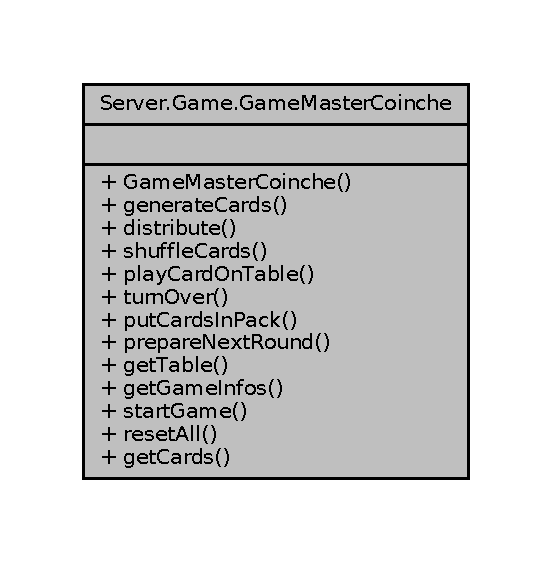
\includegraphics[width=265pt]{classServer_1_1Game_1_1GameMasterCoinche__coll__graph}
\end{center}
\end{figure}
\subsection*{Public Member Functions}
\begin{DoxyCompactItemize}
\item 
\mbox{\hyperlink{classServer_1_1Game_1_1GameMasterCoinche_aef694858e79e57155aed473c576a0527}{Game\+Master\+Coinche}} ()
\item 
void \mbox{\hyperlink{classServer_1_1Game_1_1GameMasterCoinche_a0f665b812c52453acdcfbdcf4e3b4658}{generate\+Cards}} ()
\item 
void \mbox{\hyperlink{classServer_1_1Game_1_1GameMasterCoinche_a99ce3630f1b23a97e1204f3c8744a208}{distribute}} (\mbox{\hyperlink{classServer_1_1ServerConnexion_1_1Room}{Room}} room)
\item 
void \mbox{\hyperlink{classServer_1_1Game_1_1GameMasterCoinche_acad3139f08fe5fc91ab79058530fcacf}{shuffle\+Cards}} ()
\item 
void \mbox{\hyperlink{classServer_1_1Game_1_1GameMasterCoinche_ad38b48bd930dd77a40f8c4fb28e8be17}{play\+Card\+On\+Table}} (\mbox{\hyperlink{classServer_1_1ServerConnexion_1_1ClientInfos}{Client\+Infos}} client, \mbox{\hyperlink{classCommon_1_1Card}{Card}} card)
\item 
\mbox{\hyperlink{classServer_1_1ServerConnexion_1_1ClientInfos}{Client\+Infos}} \mbox{\hyperlink{classServer_1_1Game_1_1GameMasterCoinche_a67214548e20a86dae287e8bf2c8a39d2}{turn\+Over}} ()
\item 
void \mbox{\hyperlink{classServer_1_1Game_1_1GameMasterCoinche_a53c0c498118ce3ac3168c5fc5f5520a6}{put\+Cards\+In\+Pack}} ()
\item 
void \mbox{\hyperlink{classServer_1_1Game_1_1GameMasterCoinche_a8c8b4fbd409a875500260ab34c8be1d5}{prepare\+Next\+Round}} ()
\item 
Hash\+Map$<$ \mbox{\hyperlink{classServer_1_1ServerConnexion_1_1ClientInfos}{Client\+Infos}}, \mbox{\hyperlink{classCommon_1_1Card}{Card}} $>$ \mbox{\hyperlink{classServer_1_1Game_1_1GameMasterCoinche_a44c8d2d0d299abe2810cb261fb389003}{get\+Table}} ()
\item 
\mbox{\hyperlink{classServer_1_1Game_1_1GameInfos}{Game\+Infos}} \mbox{\hyperlink{classServer_1_1Game_1_1GameMasterCoinche_af1232b7545c2e7253eddc6446178e2ba}{get\+Game\+Infos}} ()
\item 
void \mbox{\hyperlink{classServer_1_1Game_1_1GameMasterCoinche_a7b7262936aafc0600b8a456e7bd6a82f}{start\+Game}} (\mbox{\hyperlink{classServer_1_1ServerConnexion_1_1Room}{Room}} room)
\item 
void \mbox{\hyperlink{classServer_1_1Game_1_1GameMasterCoinche_a6dc593f52ebb75474aa72e4dfeba2a6d}{reset\+All}} ()
\item 
Array\+List$<$ \mbox{\hyperlink{classCommon_1_1Card}{Card}} $>$ \mbox{\hyperlink{classServer_1_1Game_1_1GameMasterCoinche_a82a6f6b6d3ba413af859546bfdfcb662}{get\+Cards}} ()
\end{DoxyCompactItemize}


\subsection{Constructor \& Destructor Documentation}
\mbox{\Hypertarget{classServer_1_1Game_1_1GameMasterCoinche_aef694858e79e57155aed473c576a0527}\label{classServer_1_1Game_1_1GameMasterCoinche_aef694858e79e57155aed473c576a0527}} 
\index{Server\+::\+Game\+::\+Game\+Master\+Coinche@{Server\+::\+Game\+::\+Game\+Master\+Coinche}!Game\+Master\+Coinche@{Game\+Master\+Coinche}}
\index{Game\+Master\+Coinche@{Game\+Master\+Coinche}!Server\+::\+Game\+::\+Game\+Master\+Coinche@{Server\+::\+Game\+::\+Game\+Master\+Coinche}}
\subsubsection{\texorpdfstring{Game\+Master\+Coinche()}{GameMasterCoinche()}}
{\footnotesize\ttfamily Server.\+Game.\+Game\+Master\+Coinche.\+Game\+Master\+Coinche (\begin{DoxyParamCaption}{ }\end{DoxyParamCaption})\hspace{0.3cm}{\ttfamily [inline]}}



\subsection{Member Function Documentation}
\mbox{\Hypertarget{classServer_1_1Game_1_1GameMasterCoinche_a99ce3630f1b23a97e1204f3c8744a208}\label{classServer_1_1Game_1_1GameMasterCoinche_a99ce3630f1b23a97e1204f3c8744a208}} 
\index{Server\+::\+Game\+::\+Game\+Master\+Coinche@{Server\+::\+Game\+::\+Game\+Master\+Coinche}!distribute@{distribute}}
\index{distribute@{distribute}!Server\+::\+Game\+::\+Game\+Master\+Coinche@{Server\+::\+Game\+::\+Game\+Master\+Coinche}}
\subsubsection{\texorpdfstring{distribute()}{distribute()}}
{\footnotesize\ttfamily void Server.\+Game.\+Game\+Master\+Coinche.\+distribute (\begin{DoxyParamCaption}\item[{\mbox{\hyperlink{classServer_1_1ServerConnexion_1_1Room}{Room}}}]{room }\end{DoxyParamCaption})\hspace{0.3cm}{\ttfamily [inline]}}

\mbox{\Hypertarget{classServer_1_1Game_1_1GameMasterCoinche_a0f665b812c52453acdcfbdcf4e3b4658}\label{classServer_1_1Game_1_1GameMasterCoinche_a0f665b812c52453acdcfbdcf4e3b4658}} 
\index{Server\+::\+Game\+::\+Game\+Master\+Coinche@{Server\+::\+Game\+::\+Game\+Master\+Coinche}!generate\+Cards@{generate\+Cards}}
\index{generate\+Cards@{generate\+Cards}!Server\+::\+Game\+::\+Game\+Master\+Coinche@{Server\+::\+Game\+::\+Game\+Master\+Coinche}}
\subsubsection{\texorpdfstring{generate\+Cards()}{generateCards()}}
{\footnotesize\ttfamily void Server.\+Game.\+Game\+Master\+Coinche.\+generate\+Cards (\begin{DoxyParamCaption}{ }\end{DoxyParamCaption})\hspace{0.3cm}{\ttfamily [inline]}}

\mbox{\Hypertarget{classServer_1_1Game_1_1GameMasterCoinche_a82a6f6b6d3ba413af859546bfdfcb662}\label{classServer_1_1Game_1_1GameMasterCoinche_a82a6f6b6d3ba413af859546bfdfcb662}} 
\index{Server\+::\+Game\+::\+Game\+Master\+Coinche@{Server\+::\+Game\+::\+Game\+Master\+Coinche}!get\+Cards@{get\+Cards}}
\index{get\+Cards@{get\+Cards}!Server\+::\+Game\+::\+Game\+Master\+Coinche@{Server\+::\+Game\+::\+Game\+Master\+Coinche}}
\subsubsection{\texorpdfstring{get\+Cards()}{getCards()}}
{\footnotesize\ttfamily Array\+List$<$\mbox{\hyperlink{classCommon_1_1Card}{Card}}$>$ Server.\+Game.\+Game\+Master\+Coinche.\+get\+Cards (\begin{DoxyParamCaption}{ }\end{DoxyParamCaption})\hspace{0.3cm}{\ttfamily [inline]}}

\mbox{\Hypertarget{classServer_1_1Game_1_1GameMasterCoinche_af1232b7545c2e7253eddc6446178e2ba}\label{classServer_1_1Game_1_1GameMasterCoinche_af1232b7545c2e7253eddc6446178e2ba}} 
\index{Server\+::\+Game\+::\+Game\+Master\+Coinche@{Server\+::\+Game\+::\+Game\+Master\+Coinche}!get\+Game\+Infos@{get\+Game\+Infos}}
\index{get\+Game\+Infos@{get\+Game\+Infos}!Server\+::\+Game\+::\+Game\+Master\+Coinche@{Server\+::\+Game\+::\+Game\+Master\+Coinche}}
\subsubsection{\texorpdfstring{get\+Game\+Infos()}{getGameInfos()}}
{\footnotesize\ttfamily \mbox{\hyperlink{classServer_1_1Game_1_1GameInfos}{Game\+Infos}} Server.\+Game.\+Game\+Master\+Coinche.\+get\+Game\+Infos (\begin{DoxyParamCaption}{ }\end{DoxyParamCaption})\hspace{0.3cm}{\ttfamily [inline]}}

\mbox{\Hypertarget{classServer_1_1Game_1_1GameMasterCoinche_a44c8d2d0d299abe2810cb261fb389003}\label{classServer_1_1Game_1_1GameMasterCoinche_a44c8d2d0d299abe2810cb261fb389003}} 
\index{Server\+::\+Game\+::\+Game\+Master\+Coinche@{Server\+::\+Game\+::\+Game\+Master\+Coinche}!get\+Table@{get\+Table}}
\index{get\+Table@{get\+Table}!Server\+::\+Game\+::\+Game\+Master\+Coinche@{Server\+::\+Game\+::\+Game\+Master\+Coinche}}
\subsubsection{\texorpdfstring{get\+Table()}{getTable()}}
{\footnotesize\ttfamily Hash\+Map$<$\mbox{\hyperlink{classServer_1_1ServerConnexion_1_1ClientInfos}{Client\+Infos}}, \mbox{\hyperlink{classCommon_1_1Card}{Card}}$>$ Server.\+Game.\+Game\+Master\+Coinche.\+get\+Table (\begin{DoxyParamCaption}{ }\end{DoxyParamCaption})\hspace{0.3cm}{\ttfamily [inline]}}

\mbox{\Hypertarget{classServer_1_1Game_1_1GameMasterCoinche_ad38b48bd930dd77a40f8c4fb28e8be17}\label{classServer_1_1Game_1_1GameMasterCoinche_ad38b48bd930dd77a40f8c4fb28e8be17}} 
\index{Server\+::\+Game\+::\+Game\+Master\+Coinche@{Server\+::\+Game\+::\+Game\+Master\+Coinche}!play\+Card\+On\+Table@{play\+Card\+On\+Table}}
\index{play\+Card\+On\+Table@{play\+Card\+On\+Table}!Server\+::\+Game\+::\+Game\+Master\+Coinche@{Server\+::\+Game\+::\+Game\+Master\+Coinche}}
\subsubsection{\texorpdfstring{play\+Card\+On\+Table()}{playCardOnTable()}}
{\footnotesize\ttfamily void Server.\+Game.\+Game\+Master\+Coinche.\+play\+Card\+On\+Table (\begin{DoxyParamCaption}\item[{\mbox{\hyperlink{classServer_1_1ServerConnexion_1_1ClientInfos}{Client\+Infos}}}]{client,  }\item[{\mbox{\hyperlink{classCommon_1_1Card}{Card}}}]{card }\end{DoxyParamCaption})\hspace{0.3cm}{\ttfamily [inline]}}

\mbox{\Hypertarget{classServer_1_1Game_1_1GameMasterCoinche_a8c8b4fbd409a875500260ab34c8be1d5}\label{classServer_1_1Game_1_1GameMasterCoinche_a8c8b4fbd409a875500260ab34c8be1d5}} 
\index{Server\+::\+Game\+::\+Game\+Master\+Coinche@{Server\+::\+Game\+::\+Game\+Master\+Coinche}!prepare\+Next\+Round@{prepare\+Next\+Round}}
\index{prepare\+Next\+Round@{prepare\+Next\+Round}!Server\+::\+Game\+::\+Game\+Master\+Coinche@{Server\+::\+Game\+::\+Game\+Master\+Coinche}}
\subsubsection{\texorpdfstring{prepare\+Next\+Round()}{prepareNextRound()}}
{\footnotesize\ttfamily void Server.\+Game.\+Game\+Master\+Coinche.\+prepare\+Next\+Round (\begin{DoxyParamCaption}{ }\end{DoxyParamCaption})\hspace{0.3cm}{\ttfamily [inline]}}

\mbox{\Hypertarget{classServer_1_1Game_1_1GameMasterCoinche_a53c0c498118ce3ac3168c5fc5f5520a6}\label{classServer_1_1Game_1_1GameMasterCoinche_a53c0c498118ce3ac3168c5fc5f5520a6}} 
\index{Server\+::\+Game\+::\+Game\+Master\+Coinche@{Server\+::\+Game\+::\+Game\+Master\+Coinche}!put\+Cards\+In\+Pack@{put\+Cards\+In\+Pack}}
\index{put\+Cards\+In\+Pack@{put\+Cards\+In\+Pack}!Server\+::\+Game\+::\+Game\+Master\+Coinche@{Server\+::\+Game\+::\+Game\+Master\+Coinche}}
\subsubsection{\texorpdfstring{put\+Cards\+In\+Pack()}{putCardsInPack()}}
{\footnotesize\ttfamily void Server.\+Game.\+Game\+Master\+Coinche.\+put\+Cards\+In\+Pack (\begin{DoxyParamCaption}{ }\end{DoxyParamCaption})\hspace{0.3cm}{\ttfamily [inline]}}

\mbox{\Hypertarget{classServer_1_1Game_1_1GameMasterCoinche_a6dc593f52ebb75474aa72e4dfeba2a6d}\label{classServer_1_1Game_1_1GameMasterCoinche_a6dc593f52ebb75474aa72e4dfeba2a6d}} 
\index{Server\+::\+Game\+::\+Game\+Master\+Coinche@{Server\+::\+Game\+::\+Game\+Master\+Coinche}!reset\+All@{reset\+All}}
\index{reset\+All@{reset\+All}!Server\+::\+Game\+::\+Game\+Master\+Coinche@{Server\+::\+Game\+::\+Game\+Master\+Coinche}}
\subsubsection{\texorpdfstring{reset\+All()}{resetAll()}}
{\footnotesize\ttfamily void Server.\+Game.\+Game\+Master\+Coinche.\+reset\+All (\begin{DoxyParamCaption}{ }\end{DoxyParamCaption})\hspace{0.3cm}{\ttfamily [inline]}}

\mbox{\Hypertarget{classServer_1_1Game_1_1GameMasterCoinche_acad3139f08fe5fc91ab79058530fcacf}\label{classServer_1_1Game_1_1GameMasterCoinche_acad3139f08fe5fc91ab79058530fcacf}} 
\index{Server\+::\+Game\+::\+Game\+Master\+Coinche@{Server\+::\+Game\+::\+Game\+Master\+Coinche}!shuffle\+Cards@{shuffle\+Cards}}
\index{shuffle\+Cards@{shuffle\+Cards}!Server\+::\+Game\+::\+Game\+Master\+Coinche@{Server\+::\+Game\+::\+Game\+Master\+Coinche}}
\subsubsection{\texorpdfstring{shuffle\+Cards()}{shuffleCards()}}
{\footnotesize\ttfamily void Server.\+Game.\+Game\+Master\+Coinche.\+shuffle\+Cards (\begin{DoxyParamCaption}{ }\end{DoxyParamCaption})\hspace{0.3cm}{\ttfamily [inline]}}

\mbox{\Hypertarget{classServer_1_1Game_1_1GameMasterCoinche_a7b7262936aafc0600b8a456e7bd6a82f}\label{classServer_1_1Game_1_1GameMasterCoinche_a7b7262936aafc0600b8a456e7bd6a82f}} 
\index{Server\+::\+Game\+::\+Game\+Master\+Coinche@{Server\+::\+Game\+::\+Game\+Master\+Coinche}!start\+Game@{start\+Game}}
\index{start\+Game@{start\+Game}!Server\+::\+Game\+::\+Game\+Master\+Coinche@{Server\+::\+Game\+::\+Game\+Master\+Coinche}}
\subsubsection{\texorpdfstring{start\+Game()}{startGame()}}
{\footnotesize\ttfamily void Server.\+Game.\+Game\+Master\+Coinche.\+start\+Game (\begin{DoxyParamCaption}\item[{\mbox{\hyperlink{classServer_1_1ServerConnexion_1_1Room}{Room}}}]{room }\end{DoxyParamCaption})\hspace{0.3cm}{\ttfamily [inline]}}

\mbox{\Hypertarget{classServer_1_1Game_1_1GameMasterCoinche_a67214548e20a86dae287e8bf2c8a39d2}\label{classServer_1_1Game_1_1GameMasterCoinche_a67214548e20a86dae287e8bf2c8a39d2}} 
\index{Server\+::\+Game\+::\+Game\+Master\+Coinche@{Server\+::\+Game\+::\+Game\+Master\+Coinche}!turn\+Over@{turn\+Over}}
\index{turn\+Over@{turn\+Over}!Server\+::\+Game\+::\+Game\+Master\+Coinche@{Server\+::\+Game\+::\+Game\+Master\+Coinche}}
\subsubsection{\texorpdfstring{turn\+Over()}{turnOver()}}
{\footnotesize\ttfamily \mbox{\hyperlink{classServer_1_1ServerConnexion_1_1ClientInfos}{Client\+Infos}} Server.\+Game.\+Game\+Master\+Coinche.\+turn\+Over (\begin{DoxyParamCaption}{ }\end{DoxyParamCaption})\hspace{0.3cm}{\ttfamily [inline]}}



The documentation for this class was generated from the following file\+:\begin{DoxyCompactItemize}
\item 
/home/tetard/\+Idea\+Projects/j\+Coinche/\+Java\+\_\+jcoinche\+\_\+2017/src/main/java/\+Server/\+Game/\mbox{\hyperlink{GameMasterCoinche_8java}{Game\+Master\+Coinche.\+java}}\end{DoxyCompactItemize}

\hypertarget{classCommon_1_1GameOverPoints}{}\section{Common.\+Game\+Over\+Points Class Reference}
\label{classCommon_1_1GameOverPoints}\index{Common.\+Game\+Over\+Points@{Common.\+Game\+Over\+Points}}


Collaboration diagram for Common.\+Game\+Over\+Points\+:
\nopagebreak
\begin{figure}[H]
\begin{center}
\leavevmode
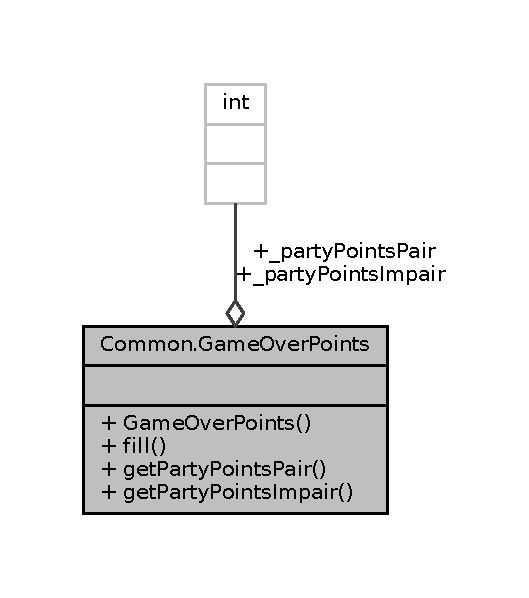
\includegraphics[width=254pt]{classCommon_1_1GameOverPoints__coll__graph}
\end{center}
\end{figure}
\subsection*{Public Member Functions}
\begin{DoxyCompactItemize}
\item 
\mbox{\hyperlink{classCommon_1_1GameOverPoints_afd6a3a2856a80e9a787ede65388d80d1}{Game\+Over\+Points}} ()
\item 
\mbox{\hyperlink{classCommon_1_1GameOverPoints}{Game\+Over\+Points}} \mbox{\hyperlink{classCommon_1_1GameOverPoints_a469f01f2db6a2e36783f9728cd91e090}{fill}} (int pair, int impair)
\item 
int \mbox{\hyperlink{classCommon_1_1GameOverPoints_a8fbb500e2039a56e94402295de1716fe}{get\+Party\+Points\+Pair}} ()
\item 
int \mbox{\hyperlink{classCommon_1_1GameOverPoints_a32908cf1b364274c562e122aedcba2ab}{get\+Party\+Points\+Impair}} ()
\end{DoxyCompactItemize}
\subsection*{Public Attributes}
\begin{DoxyCompactItemize}
\item 
int \mbox{\hyperlink{classCommon_1_1GameOverPoints_ac9113051b20fd8ee19d3750ca473f84d}{\+\_\+party\+Points\+Pair}}
\item 
int \mbox{\hyperlink{classCommon_1_1GameOverPoints_adde432d194bd142b2b2b45d4b2518c49}{\+\_\+party\+Points\+Impair}}
\end{DoxyCompactItemize}


\subsection{Constructor \& Destructor Documentation}
\mbox{\Hypertarget{classCommon_1_1GameOverPoints_afd6a3a2856a80e9a787ede65388d80d1}\label{classCommon_1_1GameOverPoints_afd6a3a2856a80e9a787ede65388d80d1}} 
\index{Common\+::\+Game\+Over\+Points@{Common\+::\+Game\+Over\+Points}!Game\+Over\+Points@{Game\+Over\+Points}}
\index{Game\+Over\+Points@{Game\+Over\+Points}!Common\+::\+Game\+Over\+Points@{Common\+::\+Game\+Over\+Points}}
\subsubsection{\texorpdfstring{Game\+Over\+Points()}{GameOverPoints()}}
{\footnotesize\ttfamily Common.\+Game\+Over\+Points.\+Game\+Over\+Points (\begin{DoxyParamCaption}{ }\end{DoxyParamCaption})\hspace{0.3cm}{\ttfamily [inline]}}



\subsection{Member Function Documentation}
\mbox{\Hypertarget{classCommon_1_1GameOverPoints_a469f01f2db6a2e36783f9728cd91e090}\label{classCommon_1_1GameOverPoints_a469f01f2db6a2e36783f9728cd91e090}} 
\index{Common\+::\+Game\+Over\+Points@{Common\+::\+Game\+Over\+Points}!fill@{fill}}
\index{fill@{fill}!Common\+::\+Game\+Over\+Points@{Common\+::\+Game\+Over\+Points}}
\subsubsection{\texorpdfstring{fill()}{fill()}}
{\footnotesize\ttfamily \mbox{\hyperlink{classCommon_1_1GameOverPoints}{Game\+Over\+Points}} Common.\+Game\+Over\+Points.\+fill (\begin{DoxyParamCaption}\item[{int}]{pair,  }\item[{int}]{impair }\end{DoxyParamCaption})\hspace{0.3cm}{\ttfamily [inline]}}

\mbox{\Hypertarget{classCommon_1_1GameOverPoints_a32908cf1b364274c562e122aedcba2ab}\label{classCommon_1_1GameOverPoints_a32908cf1b364274c562e122aedcba2ab}} 
\index{Common\+::\+Game\+Over\+Points@{Common\+::\+Game\+Over\+Points}!get\+Party\+Points\+Impair@{get\+Party\+Points\+Impair}}
\index{get\+Party\+Points\+Impair@{get\+Party\+Points\+Impair}!Common\+::\+Game\+Over\+Points@{Common\+::\+Game\+Over\+Points}}
\subsubsection{\texorpdfstring{get\+Party\+Points\+Impair()}{getPartyPointsImpair()}}
{\footnotesize\ttfamily int Common.\+Game\+Over\+Points.\+get\+Party\+Points\+Impair (\begin{DoxyParamCaption}{ }\end{DoxyParamCaption})\hspace{0.3cm}{\ttfamily [inline]}}

\mbox{\Hypertarget{classCommon_1_1GameOverPoints_a8fbb500e2039a56e94402295de1716fe}\label{classCommon_1_1GameOverPoints_a8fbb500e2039a56e94402295de1716fe}} 
\index{Common\+::\+Game\+Over\+Points@{Common\+::\+Game\+Over\+Points}!get\+Party\+Points\+Pair@{get\+Party\+Points\+Pair}}
\index{get\+Party\+Points\+Pair@{get\+Party\+Points\+Pair}!Common\+::\+Game\+Over\+Points@{Common\+::\+Game\+Over\+Points}}
\subsubsection{\texorpdfstring{get\+Party\+Points\+Pair()}{getPartyPointsPair()}}
{\footnotesize\ttfamily int Common.\+Game\+Over\+Points.\+get\+Party\+Points\+Pair (\begin{DoxyParamCaption}{ }\end{DoxyParamCaption})\hspace{0.3cm}{\ttfamily [inline]}}



\subsection{Member Data Documentation}
\mbox{\Hypertarget{classCommon_1_1GameOverPoints_adde432d194bd142b2b2b45d4b2518c49}\label{classCommon_1_1GameOverPoints_adde432d194bd142b2b2b45d4b2518c49}} 
\index{Common\+::\+Game\+Over\+Points@{Common\+::\+Game\+Over\+Points}!\+\_\+party\+Points\+Impair@{\+\_\+party\+Points\+Impair}}
\index{\+\_\+party\+Points\+Impair@{\+\_\+party\+Points\+Impair}!Common\+::\+Game\+Over\+Points@{Common\+::\+Game\+Over\+Points}}
\subsubsection{\texorpdfstring{\+\_\+party\+Points\+Impair}{\_partyPointsImpair}}
{\footnotesize\ttfamily int Common.\+Game\+Over\+Points.\+\_\+party\+Points\+Impair}

\mbox{\Hypertarget{classCommon_1_1GameOverPoints_ac9113051b20fd8ee19d3750ca473f84d}\label{classCommon_1_1GameOverPoints_ac9113051b20fd8ee19d3750ca473f84d}} 
\index{Common\+::\+Game\+Over\+Points@{Common\+::\+Game\+Over\+Points}!\+\_\+party\+Points\+Pair@{\+\_\+party\+Points\+Pair}}
\index{\+\_\+party\+Points\+Pair@{\+\_\+party\+Points\+Pair}!Common\+::\+Game\+Over\+Points@{Common\+::\+Game\+Over\+Points}}
\subsubsection{\texorpdfstring{\+\_\+party\+Points\+Pair}{\_partyPointsPair}}
{\footnotesize\ttfamily int Common.\+Game\+Over\+Points.\+\_\+party\+Points\+Pair}



The documentation for this class was generated from the following file\+:\begin{DoxyCompactItemize}
\item 
/home/tetard/\+Idea\+Projects/j\+Coinche/\+Java\+\_\+jcoinche\+\_\+2017/src/main/java/\+Common/\mbox{\hyperlink{GameOverPoints_8java}{Game\+Over\+Points.\+java}}\end{DoxyCompactItemize}

\hypertarget{classCommon_1_1IAmReady}{}\section{Common.\+I\+Am\+Ready Class Reference}
\label{classCommon_1_1IAmReady}\index{Common.\+I\+Am\+Ready@{Common.\+I\+Am\+Ready}}


Collaboration diagram for Common.\+I\+Am\+Ready\+:
\nopagebreak
\begin{figure}[H]
\begin{center}
\leavevmode
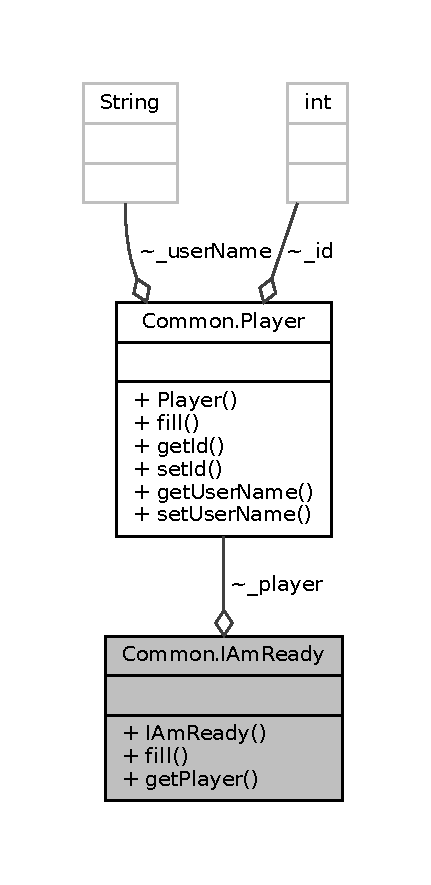
\includegraphics[width=207pt]{classCommon_1_1IAmReady__coll__graph}
\end{center}
\end{figure}
\subsection*{Public Member Functions}
\begin{DoxyCompactItemize}
\item 
\mbox{\hyperlink{classCommon_1_1IAmReady_a852717589cc197c66d331b859c43d0ed}{I\+Am\+Ready}} ()
\item 
\mbox{\hyperlink{classCommon_1_1IAmReady}{I\+Am\+Ready}} \mbox{\hyperlink{classCommon_1_1IAmReady_afb8287607db59d4e6006d7c6739604fa}{fill}} (\mbox{\hyperlink{classCommon_1_1Player}{Player}} player)
\item 
\mbox{\hyperlink{classCommon_1_1Player}{Player}} \mbox{\hyperlink{classCommon_1_1IAmReady_ad4ca10a7f3e52aa2f032d755d68e79d6}{get\+Player}} ()
\end{DoxyCompactItemize}


\subsection{Constructor \& Destructor Documentation}
\mbox{\Hypertarget{classCommon_1_1IAmReady_a852717589cc197c66d331b859c43d0ed}\label{classCommon_1_1IAmReady_a852717589cc197c66d331b859c43d0ed}} 
\index{Common\+::\+I\+Am\+Ready@{Common\+::\+I\+Am\+Ready}!I\+Am\+Ready@{I\+Am\+Ready}}
\index{I\+Am\+Ready@{I\+Am\+Ready}!Common\+::\+I\+Am\+Ready@{Common\+::\+I\+Am\+Ready}}
\subsubsection{\texorpdfstring{I\+Am\+Ready()}{IAmReady()}}
{\footnotesize\ttfamily Common.\+I\+Am\+Ready.\+I\+Am\+Ready (\begin{DoxyParamCaption}{ }\end{DoxyParamCaption})\hspace{0.3cm}{\ttfamily [inline]}}



\subsection{Member Function Documentation}
\mbox{\Hypertarget{classCommon_1_1IAmReady_afb8287607db59d4e6006d7c6739604fa}\label{classCommon_1_1IAmReady_afb8287607db59d4e6006d7c6739604fa}} 
\index{Common\+::\+I\+Am\+Ready@{Common\+::\+I\+Am\+Ready}!fill@{fill}}
\index{fill@{fill}!Common\+::\+I\+Am\+Ready@{Common\+::\+I\+Am\+Ready}}
\subsubsection{\texorpdfstring{fill()}{fill()}}
{\footnotesize\ttfamily \mbox{\hyperlink{classCommon_1_1IAmReady}{I\+Am\+Ready}} Common.\+I\+Am\+Ready.\+fill (\begin{DoxyParamCaption}\item[{\mbox{\hyperlink{classCommon_1_1Player}{Player}}}]{player }\end{DoxyParamCaption})\hspace{0.3cm}{\ttfamily [inline]}}

\mbox{\Hypertarget{classCommon_1_1IAmReady_ad4ca10a7f3e52aa2f032d755d68e79d6}\label{classCommon_1_1IAmReady_ad4ca10a7f3e52aa2f032d755d68e79d6}} 
\index{Common\+::\+I\+Am\+Ready@{Common\+::\+I\+Am\+Ready}!get\+Player@{get\+Player}}
\index{get\+Player@{get\+Player}!Common\+::\+I\+Am\+Ready@{Common\+::\+I\+Am\+Ready}}
\subsubsection{\texorpdfstring{get\+Player()}{getPlayer()}}
{\footnotesize\ttfamily \mbox{\hyperlink{classCommon_1_1Player}{Player}} Common.\+I\+Am\+Ready.\+get\+Player (\begin{DoxyParamCaption}{ }\end{DoxyParamCaption})\hspace{0.3cm}{\ttfamily [inline]}}



The documentation for this class was generated from the following file\+:\begin{DoxyCompactItemize}
\item 
/home/tetard/\+Idea\+Projects/j\+Coinche/\+Java\+\_\+jcoinche\+\_\+2017/src/main/java/\+Common/\mbox{\hyperlink{IAmReady_8java}{I\+Am\+Ready.\+java}}\end{DoxyCompactItemize}

\hypertarget{classClient_1_1Model_1_1InstanceModel}{}\section{Client.\+Model.\+Instance\+Model Class Reference}
\label{classClient_1_1Model_1_1InstanceModel}\index{Client.\+Model.\+Instance\+Model@{Client.\+Model.\+Instance\+Model}}


Inheritance diagram for Client.\+Model.\+Instance\+Model\+:
\nopagebreak
\begin{figure}[H]
\begin{center}
\leavevmode
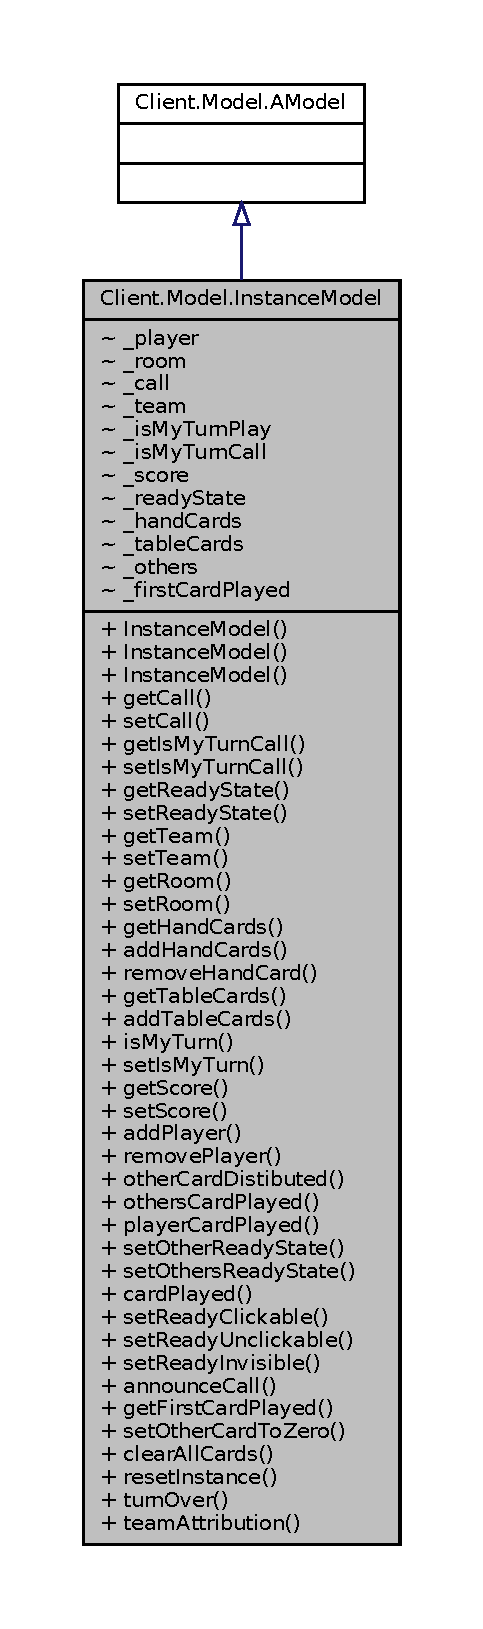
\includegraphics[height=550pt]{classClient_1_1Model_1_1InstanceModel__inherit__graph}
\end{center}
\end{figure}


Collaboration diagram for Client.\+Model.\+Instance\+Model\+:
\nopagebreak
\begin{figure}[H]
\begin{center}
\leavevmode
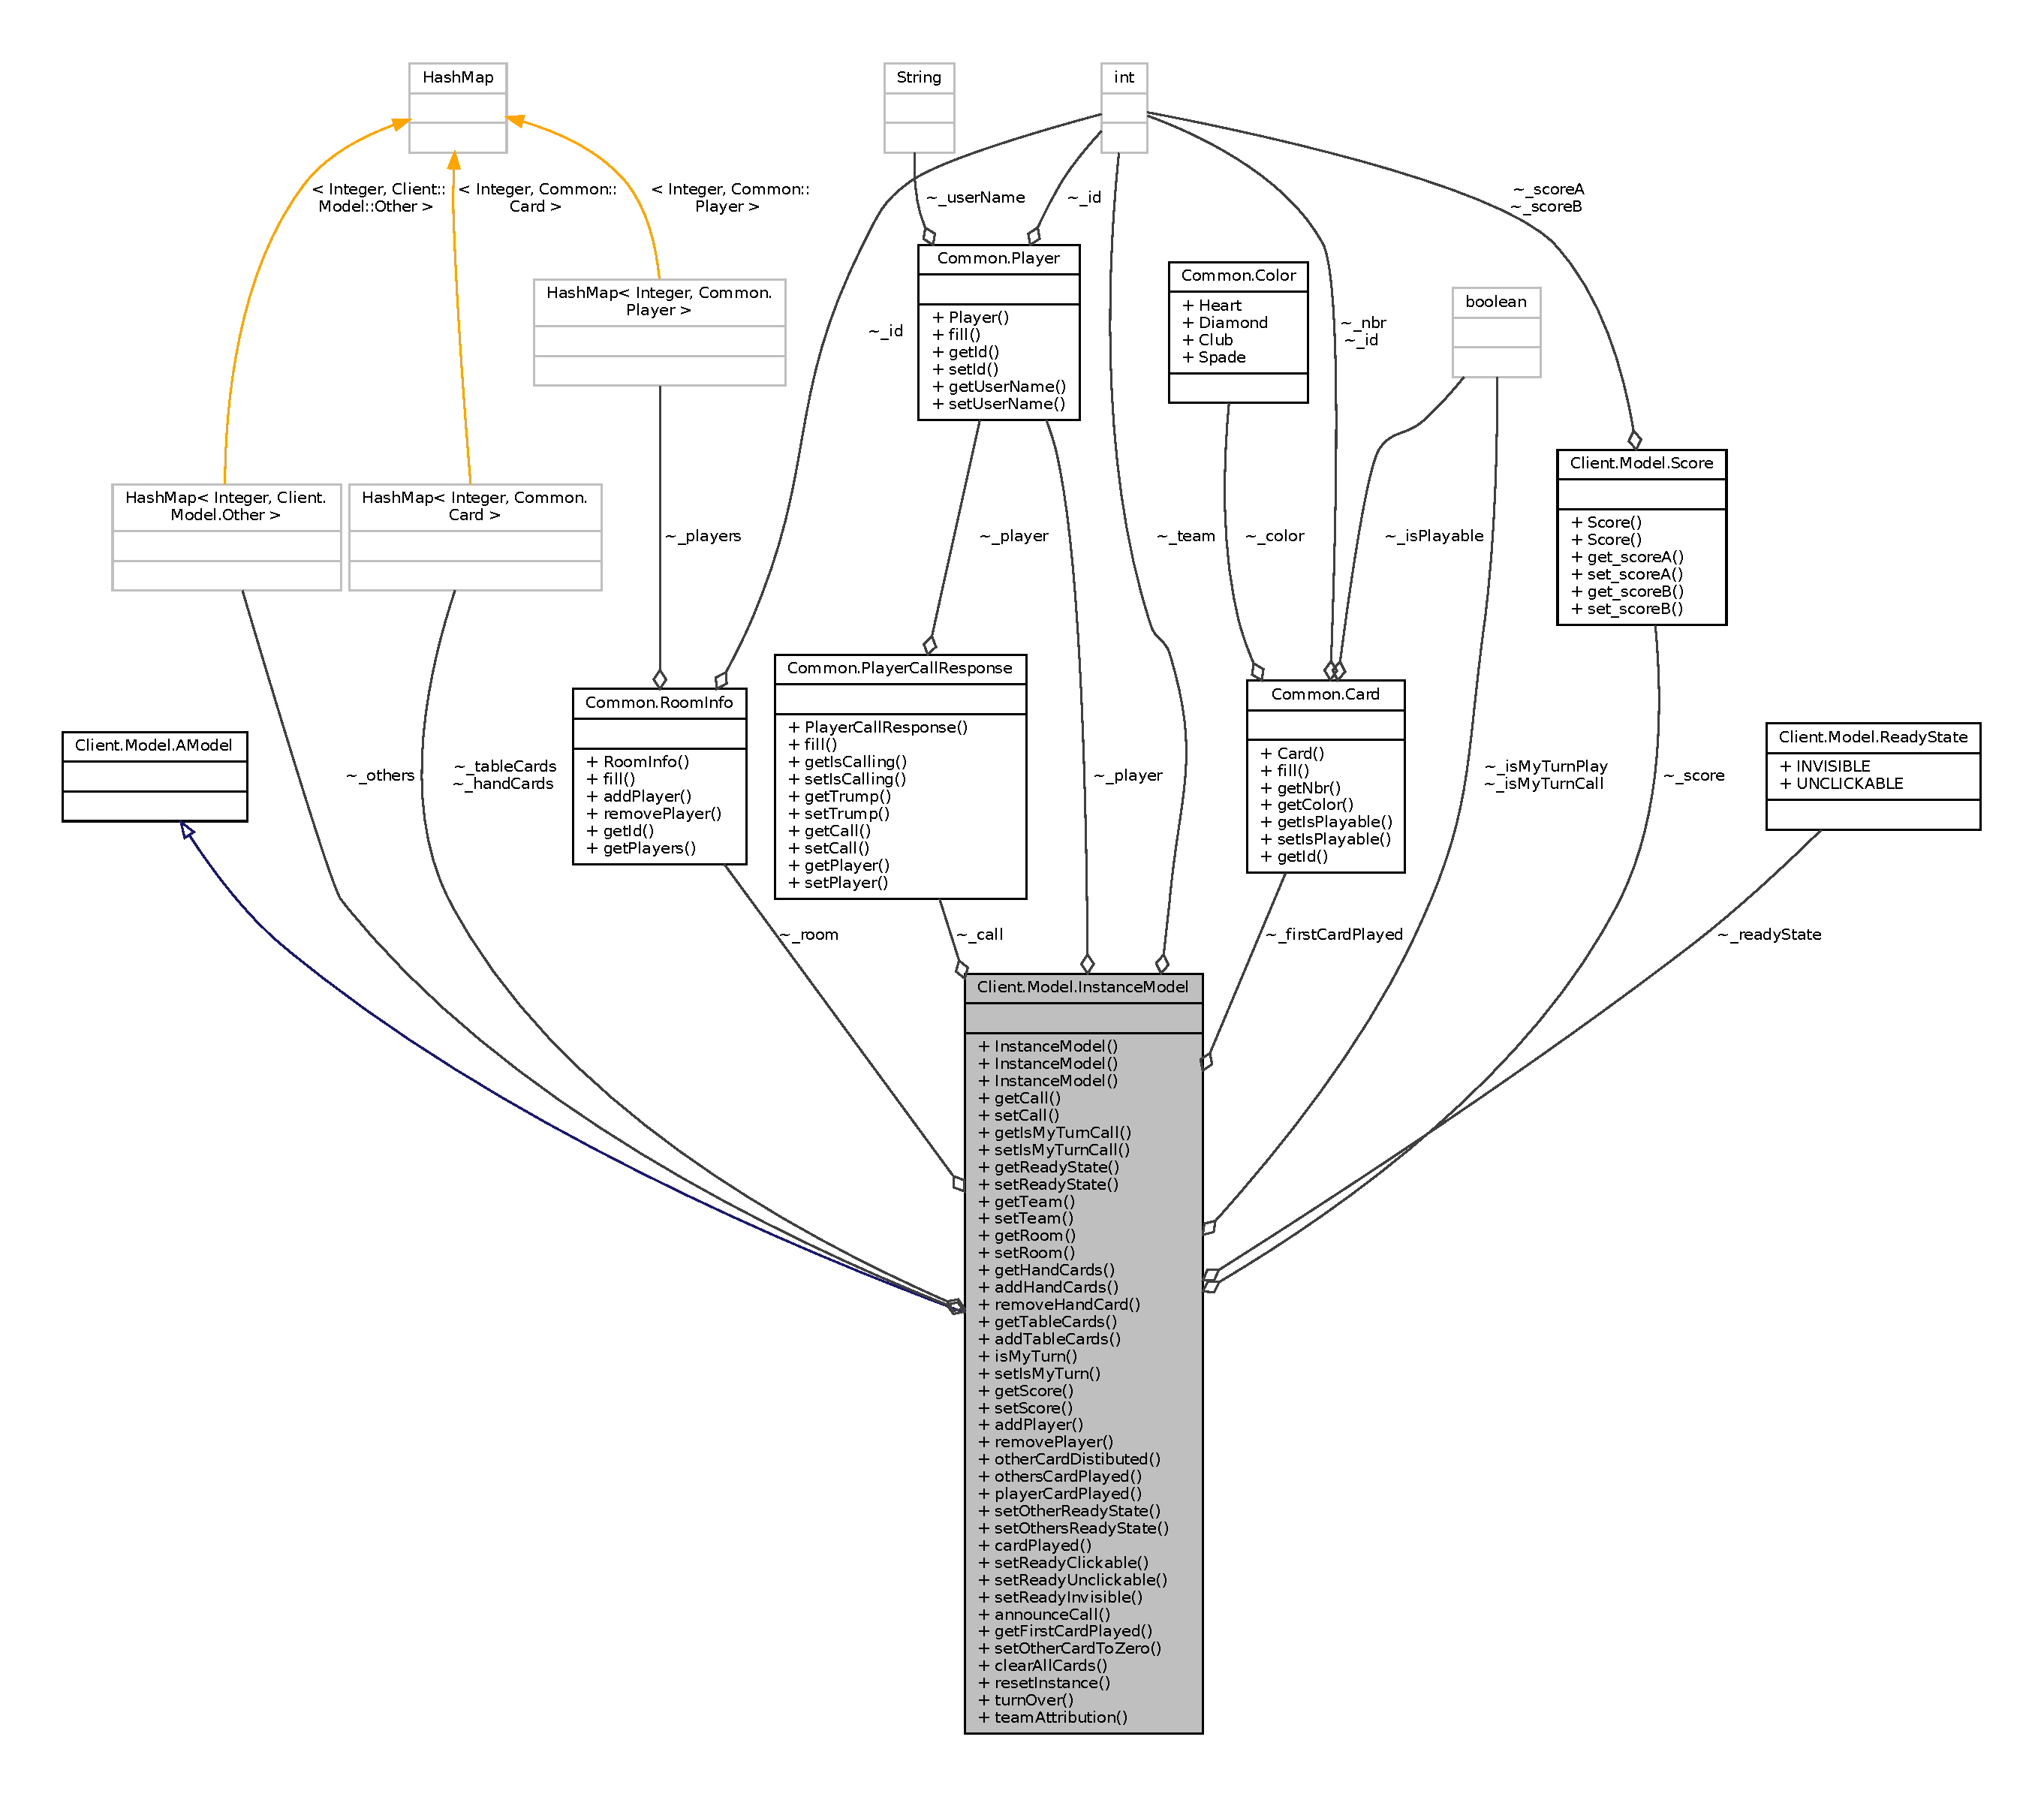
\includegraphics[width=350pt]{classClient_1_1Model_1_1InstanceModel__coll__graph}
\end{center}
\end{figure}
\subsection*{Public Member Functions}
\begin{DoxyCompactItemize}
\item 
\mbox{\hyperlink{classClient_1_1Model_1_1InstanceModel_ad2f61d837a1d5b806b772d8a4a7430d8}{Instance\+Model}} (\mbox{\hyperlink{classCommon_1_1Player}{Player}} player, \mbox{\hyperlink{classCommon_1_1RoomInfo}{Room\+Info}} room)
\item 
\mbox{\hyperlink{classClient_1_1Model_1_1InstanceModel_acb00a285b30ad1851157852624d59499}{Instance\+Model}} (\mbox{\hyperlink{classCommon_1_1PlayerCallResponse}{Player\+Call\+Response}} call, Hash\+Map$<$ Integer, \mbox{\hyperlink{classCommon_1_1Card}{Card}} $>$ hand\+Cards, Hash\+Map$<$ Integer, \mbox{\hyperlink{classCommon_1_1Card}{Card}} $>$ table\+Cards, \mbox{\hyperlink{classCommon_1_1Card}{Card}} first)
\item 
\mbox{\hyperlink{classClient_1_1Model_1_1InstanceModel_a5393980d2fb01dd6bc13f88cbabb77f6}{Instance\+Model}} ()
\item 
\mbox{\hyperlink{classCommon_1_1PlayerCallResponse}{Player\+Call\+Response}} \mbox{\hyperlink{classClient_1_1Model_1_1InstanceModel_ad8583f69e6b0ca17a8a5849d1a6b72a3}{get\+Call}} ()
\item 
void \mbox{\hyperlink{classClient_1_1Model_1_1InstanceModel_a4ed6be9a9f752d23d38ff629bddf8c91}{set\+Call}} (\mbox{\hyperlink{classCommon_1_1PlayerCallResponse}{Player\+Call\+Response}} call)
\item 
boolean \mbox{\hyperlink{classClient_1_1Model_1_1InstanceModel_a41b625348d1dcd894b8f73b008d01d2f}{get\+Is\+My\+Turn\+Call}} ()
\item 
void \mbox{\hyperlink{classClient_1_1Model_1_1InstanceModel_a5dc1aac45a8a26c54f9a24ab791c94f9}{set\+Is\+My\+Turn\+Call}} (boolean is\+My\+Turn\+Call)
\item 
\mbox{\hyperlink{enumClient_1_1Model_1_1ReadyState}{Ready\+State}} \mbox{\hyperlink{classClient_1_1Model_1_1InstanceModel_acddabd74d9ec0d00b08f5fdbb84bb609}{get\+Ready\+State}} ()
\item 
void \mbox{\hyperlink{classClient_1_1Model_1_1InstanceModel_ae5d961affa08986ceedd6b771d740078}{set\+Ready\+State}} (\mbox{\hyperlink{enumClient_1_1Model_1_1ReadyState}{Ready\+State}} state)
\item 
int \mbox{\hyperlink{classClient_1_1Model_1_1InstanceModel_ab08b70b054c7c55685ea24af1dd25914}{get\+Team}} ()
\item 
void \mbox{\hyperlink{classClient_1_1Model_1_1InstanceModel_a7a6b8e1bf99e71a855e91dbd3b79ef21}{set\+Team}} (int team)
\item 
\mbox{\hyperlink{classCommon_1_1RoomInfo}{Room\+Info}} \mbox{\hyperlink{classClient_1_1Model_1_1InstanceModel_a6f42d7fdb1ff144f4dac43d286db3515}{get\+Room}} ()
\item 
void \mbox{\hyperlink{classClient_1_1Model_1_1InstanceModel_ad383951ca582c2b93e56cab76da7a50d}{set\+Room}} (\mbox{\hyperlink{classCommon_1_1RoomInfo}{Room\+Info}} room)
\item 
Hash\+Map$<$ Integer, \mbox{\hyperlink{classCommon_1_1Card}{Card}} $>$ \mbox{\hyperlink{classClient_1_1Model_1_1InstanceModel_ab9869708057146636b1773389c1ff58b}{get\+Hand\+Cards}} ()
\item 
void \mbox{\hyperlink{classClient_1_1Model_1_1InstanceModel_a8a2f49da7c74662a49caf91450d53e3e}{add\+Hand\+Cards}} (\mbox{\hyperlink{classCommon_1_1Card}{Card}} card)
\item 
void \mbox{\hyperlink{classClient_1_1Model_1_1InstanceModel_a3b6a2963467530846c5176b3c74d14ed}{remove\+Hand\+Card}} (\mbox{\hyperlink{classCommon_1_1Card}{Card}} card)
\item 
Hash\+Map$<$ Integer, \mbox{\hyperlink{classCommon_1_1Card}{Card}} $>$ \mbox{\hyperlink{classClient_1_1Model_1_1InstanceModel_a96126216a891878666841d1cad7f2efa}{get\+Table\+Cards}} ()
\item 
void \mbox{\hyperlink{classClient_1_1Model_1_1InstanceModel_aafa39746b9d039592d4c68e201ac1016}{add\+Table\+Cards}} (\mbox{\hyperlink{classCommon_1_1Card}{Card}} card)
\item 
boolean \mbox{\hyperlink{classClient_1_1Model_1_1InstanceModel_a355194b190bd46f5d32471adfc7a73c4}{is\+My\+Turn}} ()
\item 
void \mbox{\hyperlink{classClient_1_1Model_1_1InstanceModel_a10f6f136d3f04b9c9c2df29de44cd9fc}{set\+Is\+My\+Turn}} (boolean is\+My\+Turn\+Play)
\item 
\mbox{\hyperlink{classClient_1_1Model_1_1Score}{Score}} \mbox{\hyperlink{classClient_1_1Model_1_1InstanceModel_a80042ebca2c9a690878aa98492f10d02}{get\+Score}} ()
\item 
void \mbox{\hyperlink{classClient_1_1Model_1_1InstanceModel_aa22d40552433d341db0fdb8ae292004d}{set\+Score}} (\mbox{\hyperlink{classClient_1_1Model_1_1Score}{Score}} score)
\item 
void \mbox{\hyperlink{classClient_1_1Model_1_1InstanceModel_a33b1ff3d2c7e42af3faacd8204939889}{add\+Player}} (int id)
\item 
void \mbox{\hyperlink{classClient_1_1Model_1_1InstanceModel_a09e3c3a7d7644c5269d8e5b584c9a05d}{remove\+Player}} (int id)
\item 
void \mbox{\hyperlink{classClient_1_1Model_1_1InstanceModel_a8671c478f5e9b1e6d61492b05e380fef}{other\+Card\+Distibuted}} (int id)
\item 
void \mbox{\hyperlink{classClient_1_1Model_1_1InstanceModel_abf0dd62b246d54aac6e708a129eabb3d}{others\+Card\+Played}} (int id, \mbox{\hyperlink{classCommon_1_1Card}{Card}} card)
\item 
void \mbox{\hyperlink{classClient_1_1Model_1_1InstanceModel_a39157358e9c27b16cee5eab48f7923a5}{player\+Card\+Played}} (\mbox{\hyperlink{classCommon_1_1Card}{Card}} card)
\item 
void \mbox{\hyperlink{classClient_1_1Model_1_1InstanceModel_af698a59ea2bd18bfc39f98b490aeda3a}{set\+Other\+Ready\+State}} (\mbox{\hyperlink{classCommon_1_1Player}{Player}} player, \mbox{\hyperlink{enumClient_1_1Model_1_1ReadyState}{Ready\+State}} state)
\item 
void \mbox{\hyperlink{classClient_1_1Model_1_1InstanceModel_ab9092b74c1a64f4788d300ca219ecce9}{set\+Others\+Ready\+State}} (\mbox{\hyperlink{enumClient_1_1Model_1_1ReadyState}{Ready\+State}} state)
\item 
void \mbox{\hyperlink{classClient_1_1Model_1_1InstanceModel_a57253fed871cdc98a72dcd2dd7770267}{card\+Played}} (\mbox{\hyperlink{classCommon_1_1Player}{Player}} player, \mbox{\hyperlink{classCommon_1_1Card}{Card}} card)
\item 
void \mbox{\hyperlink{classClient_1_1Model_1_1InstanceModel_a8d64cf17d30cf39001dc9fe8d489a214}{set\+Ready\+Clickable}} ()
\item 
void \mbox{\hyperlink{classClient_1_1Model_1_1InstanceModel_a47214f7ce49ca75c40986cac080a110e}{set\+Ready\+Unclickable}} (\mbox{\hyperlink{classCommon_1_1Player}{Player}} player)
\item 
void \mbox{\hyperlink{classClient_1_1Model_1_1InstanceModel_a424e0747d3d1de61f8ac8c3c8fd881ec}{set\+Ready\+Invisible}} ()
\item 
void \mbox{\hyperlink{classClient_1_1Model_1_1InstanceModel_aabe33dbac5182adcd97269ee5305f540}{announce\+Call}} (\mbox{\hyperlink{classCommon_1_1PlayerCallResponse}{Player\+Call\+Response}} call)
\item 
\mbox{\hyperlink{classCommon_1_1Card}{Card}} \mbox{\hyperlink{classClient_1_1Model_1_1InstanceModel_ad8571831813c7b6e51714223303a9515}{get\+First\+Card\+Played}} ()
\item 
void \mbox{\hyperlink{classClient_1_1Model_1_1InstanceModel_a2497f3fa4b9239e4d15b7ecc6e71e451}{set\+Other\+Card\+To\+Zero}} ()
\item 
void \mbox{\hyperlink{classClient_1_1Model_1_1InstanceModel_a88f9dcbbcb9095e04548af160d361bf0}{clear\+All\+Cards}} ()
\item 
void \mbox{\hyperlink{classClient_1_1Model_1_1InstanceModel_aa6cbe5a7384a553633925542d2d03982}{reset\+Instance}} ()
\item 
void \mbox{\hyperlink{classClient_1_1Model_1_1InstanceModel_a5d3dbc02d71df092c92de89e94ba3fff}{turn\+Over}} (\mbox{\hyperlink{classCommon_1_1TurnOver}{Turn\+Over}} turn\+Over)
\item 
void \mbox{\hyperlink{classClient_1_1Model_1_1InstanceModel_a36b2da19e784f1822d27b2803a0e3f2e}{team\+Attribution}} (\mbox{\hyperlink{classCommon_1_1TeamAttribution}{Team\+Attribution}} team\+Attribution)
\end{DoxyCompactItemize}


\subsection{Constructor \& Destructor Documentation}
\mbox{\Hypertarget{classClient_1_1Model_1_1InstanceModel_ad2f61d837a1d5b806b772d8a4a7430d8}\label{classClient_1_1Model_1_1InstanceModel_ad2f61d837a1d5b806b772d8a4a7430d8}} 
\index{Client\+::\+Model\+::\+Instance\+Model@{Client\+::\+Model\+::\+Instance\+Model}!Instance\+Model@{Instance\+Model}}
\index{Instance\+Model@{Instance\+Model}!Client\+::\+Model\+::\+Instance\+Model@{Client\+::\+Model\+::\+Instance\+Model}}
\subsubsection{\texorpdfstring{Instance\+Model()}{InstanceModel()}\hspace{0.1cm}{\footnotesize\ttfamily [1/3]}}
{\footnotesize\ttfamily Client.\+Model.\+Instance\+Model.\+Instance\+Model (\begin{DoxyParamCaption}\item[{\mbox{\hyperlink{classCommon_1_1Player}{Player}}}]{player,  }\item[{\mbox{\hyperlink{classCommon_1_1RoomInfo}{Room\+Info}}}]{room }\end{DoxyParamCaption})\hspace{0.3cm}{\ttfamily [inline]}}

\mbox{\Hypertarget{classClient_1_1Model_1_1InstanceModel_acb00a285b30ad1851157852624d59499}\label{classClient_1_1Model_1_1InstanceModel_acb00a285b30ad1851157852624d59499}} 
\index{Client\+::\+Model\+::\+Instance\+Model@{Client\+::\+Model\+::\+Instance\+Model}!Instance\+Model@{Instance\+Model}}
\index{Instance\+Model@{Instance\+Model}!Client\+::\+Model\+::\+Instance\+Model@{Client\+::\+Model\+::\+Instance\+Model}}
\subsubsection{\texorpdfstring{Instance\+Model()}{InstanceModel()}\hspace{0.1cm}{\footnotesize\ttfamily [2/3]}}
{\footnotesize\ttfamily Client.\+Model.\+Instance\+Model.\+Instance\+Model (\begin{DoxyParamCaption}\item[{\mbox{\hyperlink{classCommon_1_1PlayerCallResponse}{Player\+Call\+Response}}}]{call,  }\item[{Hash\+Map$<$ Integer, \mbox{\hyperlink{classCommon_1_1Card}{Card}} $>$}]{hand\+Cards,  }\item[{Hash\+Map$<$ Integer, \mbox{\hyperlink{classCommon_1_1Card}{Card}} $>$}]{table\+Cards,  }\item[{\mbox{\hyperlink{classCommon_1_1Card}{Card}}}]{first }\end{DoxyParamCaption})\hspace{0.3cm}{\ttfamily [inline]}}

\mbox{\Hypertarget{classClient_1_1Model_1_1InstanceModel_a5393980d2fb01dd6bc13f88cbabb77f6}\label{classClient_1_1Model_1_1InstanceModel_a5393980d2fb01dd6bc13f88cbabb77f6}} 
\index{Client\+::\+Model\+::\+Instance\+Model@{Client\+::\+Model\+::\+Instance\+Model}!Instance\+Model@{Instance\+Model}}
\index{Instance\+Model@{Instance\+Model}!Client\+::\+Model\+::\+Instance\+Model@{Client\+::\+Model\+::\+Instance\+Model}}
\subsubsection{\texorpdfstring{Instance\+Model()}{InstanceModel()}\hspace{0.1cm}{\footnotesize\ttfamily [3/3]}}
{\footnotesize\ttfamily Client.\+Model.\+Instance\+Model.\+Instance\+Model (\begin{DoxyParamCaption}{ }\end{DoxyParamCaption})\hspace{0.3cm}{\ttfamily [inline]}}



\subsection{Member Function Documentation}
\mbox{\Hypertarget{classClient_1_1Model_1_1InstanceModel_a8a2f49da7c74662a49caf91450d53e3e}\label{classClient_1_1Model_1_1InstanceModel_a8a2f49da7c74662a49caf91450d53e3e}} 
\index{Client\+::\+Model\+::\+Instance\+Model@{Client\+::\+Model\+::\+Instance\+Model}!add\+Hand\+Cards@{add\+Hand\+Cards}}
\index{add\+Hand\+Cards@{add\+Hand\+Cards}!Client\+::\+Model\+::\+Instance\+Model@{Client\+::\+Model\+::\+Instance\+Model}}
\subsubsection{\texorpdfstring{add\+Hand\+Cards()}{addHandCards()}}
{\footnotesize\ttfamily void Client.\+Model.\+Instance\+Model.\+add\+Hand\+Cards (\begin{DoxyParamCaption}\item[{\mbox{\hyperlink{classCommon_1_1Card}{Card}}}]{card }\end{DoxyParamCaption})\hspace{0.3cm}{\ttfamily [inline]}}

\mbox{\Hypertarget{classClient_1_1Model_1_1InstanceModel_a33b1ff3d2c7e42af3faacd8204939889}\label{classClient_1_1Model_1_1InstanceModel_a33b1ff3d2c7e42af3faacd8204939889}} 
\index{Client\+::\+Model\+::\+Instance\+Model@{Client\+::\+Model\+::\+Instance\+Model}!add\+Player@{add\+Player}}
\index{add\+Player@{add\+Player}!Client\+::\+Model\+::\+Instance\+Model@{Client\+::\+Model\+::\+Instance\+Model}}
\subsubsection{\texorpdfstring{add\+Player()}{addPlayer()}}
{\footnotesize\ttfamily void Client.\+Model.\+Instance\+Model.\+add\+Player (\begin{DoxyParamCaption}\item[{int}]{id }\end{DoxyParamCaption})\hspace{0.3cm}{\ttfamily [inline]}}

\mbox{\Hypertarget{classClient_1_1Model_1_1InstanceModel_aafa39746b9d039592d4c68e201ac1016}\label{classClient_1_1Model_1_1InstanceModel_aafa39746b9d039592d4c68e201ac1016}} 
\index{Client\+::\+Model\+::\+Instance\+Model@{Client\+::\+Model\+::\+Instance\+Model}!add\+Table\+Cards@{add\+Table\+Cards}}
\index{add\+Table\+Cards@{add\+Table\+Cards}!Client\+::\+Model\+::\+Instance\+Model@{Client\+::\+Model\+::\+Instance\+Model}}
\subsubsection{\texorpdfstring{add\+Table\+Cards()}{addTableCards()}}
{\footnotesize\ttfamily void Client.\+Model.\+Instance\+Model.\+add\+Table\+Cards (\begin{DoxyParamCaption}\item[{\mbox{\hyperlink{classCommon_1_1Card}{Card}}}]{card }\end{DoxyParamCaption})\hspace{0.3cm}{\ttfamily [inline]}}

\mbox{\Hypertarget{classClient_1_1Model_1_1InstanceModel_aabe33dbac5182adcd97269ee5305f540}\label{classClient_1_1Model_1_1InstanceModel_aabe33dbac5182adcd97269ee5305f540}} 
\index{Client\+::\+Model\+::\+Instance\+Model@{Client\+::\+Model\+::\+Instance\+Model}!announce\+Call@{announce\+Call}}
\index{announce\+Call@{announce\+Call}!Client\+::\+Model\+::\+Instance\+Model@{Client\+::\+Model\+::\+Instance\+Model}}
\subsubsection{\texorpdfstring{announce\+Call()}{announceCall()}}
{\footnotesize\ttfamily void Client.\+Model.\+Instance\+Model.\+announce\+Call (\begin{DoxyParamCaption}\item[{\mbox{\hyperlink{classCommon_1_1PlayerCallResponse}{Player\+Call\+Response}}}]{call }\end{DoxyParamCaption})\hspace{0.3cm}{\ttfamily [inline]}}

\mbox{\Hypertarget{classClient_1_1Model_1_1InstanceModel_a57253fed871cdc98a72dcd2dd7770267}\label{classClient_1_1Model_1_1InstanceModel_a57253fed871cdc98a72dcd2dd7770267}} 
\index{Client\+::\+Model\+::\+Instance\+Model@{Client\+::\+Model\+::\+Instance\+Model}!card\+Played@{card\+Played}}
\index{card\+Played@{card\+Played}!Client\+::\+Model\+::\+Instance\+Model@{Client\+::\+Model\+::\+Instance\+Model}}
\subsubsection{\texorpdfstring{card\+Played()}{cardPlayed()}}
{\footnotesize\ttfamily void Client.\+Model.\+Instance\+Model.\+card\+Played (\begin{DoxyParamCaption}\item[{\mbox{\hyperlink{classCommon_1_1Player}{Player}}}]{player,  }\item[{\mbox{\hyperlink{classCommon_1_1Card}{Card}}}]{card }\end{DoxyParamCaption})\hspace{0.3cm}{\ttfamily [inline]}}

\mbox{\Hypertarget{classClient_1_1Model_1_1InstanceModel_a88f9dcbbcb9095e04548af160d361bf0}\label{classClient_1_1Model_1_1InstanceModel_a88f9dcbbcb9095e04548af160d361bf0}} 
\index{Client\+::\+Model\+::\+Instance\+Model@{Client\+::\+Model\+::\+Instance\+Model}!clear\+All\+Cards@{clear\+All\+Cards}}
\index{clear\+All\+Cards@{clear\+All\+Cards}!Client\+::\+Model\+::\+Instance\+Model@{Client\+::\+Model\+::\+Instance\+Model}}
\subsubsection{\texorpdfstring{clear\+All\+Cards()}{clearAllCards()}}
{\footnotesize\ttfamily void Client.\+Model.\+Instance\+Model.\+clear\+All\+Cards (\begin{DoxyParamCaption}{ }\end{DoxyParamCaption})\hspace{0.3cm}{\ttfamily [inline]}}

\mbox{\Hypertarget{classClient_1_1Model_1_1InstanceModel_ad8583f69e6b0ca17a8a5849d1a6b72a3}\label{classClient_1_1Model_1_1InstanceModel_ad8583f69e6b0ca17a8a5849d1a6b72a3}} 
\index{Client\+::\+Model\+::\+Instance\+Model@{Client\+::\+Model\+::\+Instance\+Model}!get\+Call@{get\+Call}}
\index{get\+Call@{get\+Call}!Client\+::\+Model\+::\+Instance\+Model@{Client\+::\+Model\+::\+Instance\+Model}}
\subsubsection{\texorpdfstring{get\+Call()}{getCall()}}
{\footnotesize\ttfamily \mbox{\hyperlink{classCommon_1_1PlayerCallResponse}{Player\+Call\+Response}} Client.\+Model.\+Instance\+Model.\+get\+Call (\begin{DoxyParamCaption}{ }\end{DoxyParamCaption})\hspace{0.3cm}{\ttfamily [inline]}}

\mbox{\Hypertarget{classClient_1_1Model_1_1InstanceModel_ad8571831813c7b6e51714223303a9515}\label{classClient_1_1Model_1_1InstanceModel_ad8571831813c7b6e51714223303a9515}} 
\index{Client\+::\+Model\+::\+Instance\+Model@{Client\+::\+Model\+::\+Instance\+Model}!get\+First\+Card\+Played@{get\+First\+Card\+Played}}
\index{get\+First\+Card\+Played@{get\+First\+Card\+Played}!Client\+::\+Model\+::\+Instance\+Model@{Client\+::\+Model\+::\+Instance\+Model}}
\subsubsection{\texorpdfstring{get\+First\+Card\+Played()}{getFirstCardPlayed()}}
{\footnotesize\ttfamily \mbox{\hyperlink{classCommon_1_1Card}{Card}} Client.\+Model.\+Instance\+Model.\+get\+First\+Card\+Played (\begin{DoxyParamCaption}{ }\end{DoxyParamCaption})\hspace{0.3cm}{\ttfamily [inline]}}

\mbox{\Hypertarget{classClient_1_1Model_1_1InstanceModel_ab9869708057146636b1773389c1ff58b}\label{classClient_1_1Model_1_1InstanceModel_ab9869708057146636b1773389c1ff58b}} 
\index{Client\+::\+Model\+::\+Instance\+Model@{Client\+::\+Model\+::\+Instance\+Model}!get\+Hand\+Cards@{get\+Hand\+Cards}}
\index{get\+Hand\+Cards@{get\+Hand\+Cards}!Client\+::\+Model\+::\+Instance\+Model@{Client\+::\+Model\+::\+Instance\+Model}}
\subsubsection{\texorpdfstring{get\+Hand\+Cards()}{getHandCards()}}
{\footnotesize\ttfamily Hash\+Map$<$Integer, \mbox{\hyperlink{classCommon_1_1Card}{Card}}$>$ Client.\+Model.\+Instance\+Model.\+get\+Hand\+Cards (\begin{DoxyParamCaption}{ }\end{DoxyParamCaption})\hspace{0.3cm}{\ttfamily [inline]}}

\mbox{\Hypertarget{classClient_1_1Model_1_1InstanceModel_a41b625348d1dcd894b8f73b008d01d2f}\label{classClient_1_1Model_1_1InstanceModel_a41b625348d1dcd894b8f73b008d01d2f}} 
\index{Client\+::\+Model\+::\+Instance\+Model@{Client\+::\+Model\+::\+Instance\+Model}!get\+Is\+My\+Turn\+Call@{get\+Is\+My\+Turn\+Call}}
\index{get\+Is\+My\+Turn\+Call@{get\+Is\+My\+Turn\+Call}!Client\+::\+Model\+::\+Instance\+Model@{Client\+::\+Model\+::\+Instance\+Model}}
\subsubsection{\texorpdfstring{get\+Is\+My\+Turn\+Call()}{getIsMyTurnCall()}}
{\footnotesize\ttfamily boolean Client.\+Model.\+Instance\+Model.\+get\+Is\+My\+Turn\+Call (\begin{DoxyParamCaption}{ }\end{DoxyParamCaption})\hspace{0.3cm}{\ttfamily [inline]}}

\mbox{\Hypertarget{classClient_1_1Model_1_1InstanceModel_acddabd74d9ec0d00b08f5fdbb84bb609}\label{classClient_1_1Model_1_1InstanceModel_acddabd74d9ec0d00b08f5fdbb84bb609}} 
\index{Client\+::\+Model\+::\+Instance\+Model@{Client\+::\+Model\+::\+Instance\+Model}!get\+Ready\+State@{get\+Ready\+State}}
\index{get\+Ready\+State@{get\+Ready\+State}!Client\+::\+Model\+::\+Instance\+Model@{Client\+::\+Model\+::\+Instance\+Model}}
\subsubsection{\texorpdfstring{get\+Ready\+State()}{getReadyState()}}
{\footnotesize\ttfamily \mbox{\hyperlink{enumClient_1_1Model_1_1ReadyState}{Ready\+State}} Client.\+Model.\+Instance\+Model.\+get\+Ready\+State (\begin{DoxyParamCaption}{ }\end{DoxyParamCaption})\hspace{0.3cm}{\ttfamily [inline]}}

\mbox{\Hypertarget{classClient_1_1Model_1_1InstanceModel_a6f42d7fdb1ff144f4dac43d286db3515}\label{classClient_1_1Model_1_1InstanceModel_a6f42d7fdb1ff144f4dac43d286db3515}} 
\index{Client\+::\+Model\+::\+Instance\+Model@{Client\+::\+Model\+::\+Instance\+Model}!get\+Room@{get\+Room}}
\index{get\+Room@{get\+Room}!Client\+::\+Model\+::\+Instance\+Model@{Client\+::\+Model\+::\+Instance\+Model}}
\subsubsection{\texorpdfstring{get\+Room()}{getRoom()}}
{\footnotesize\ttfamily \mbox{\hyperlink{classCommon_1_1RoomInfo}{Room\+Info}} Client.\+Model.\+Instance\+Model.\+get\+Room (\begin{DoxyParamCaption}{ }\end{DoxyParamCaption})\hspace{0.3cm}{\ttfamily [inline]}}

\mbox{\Hypertarget{classClient_1_1Model_1_1InstanceModel_a80042ebca2c9a690878aa98492f10d02}\label{classClient_1_1Model_1_1InstanceModel_a80042ebca2c9a690878aa98492f10d02}} 
\index{Client\+::\+Model\+::\+Instance\+Model@{Client\+::\+Model\+::\+Instance\+Model}!get\+Score@{get\+Score}}
\index{get\+Score@{get\+Score}!Client\+::\+Model\+::\+Instance\+Model@{Client\+::\+Model\+::\+Instance\+Model}}
\subsubsection{\texorpdfstring{get\+Score()}{getScore()}}
{\footnotesize\ttfamily \mbox{\hyperlink{classClient_1_1Model_1_1Score}{Score}} Client.\+Model.\+Instance\+Model.\+get\+Score (\begin{DoxyParamCaption}{ }\end{DoxyParamCaption})\hspace{0.3cm}{\ttfamily [inline]}}

\mbox{\Hypertarget{classClient_1_1Model_1_1InstanceModel_a96126216a891878666841d1cad7f2efa}\label{classClient_1_1Model_1_1InstanceModel_a96126216a891878666841d1cad7f2efa}} 
\index{Client\+::\+Model\+::\+Instance\+Model@{Client\+::\+Model\+::\+Instance\+Model}!get\+Table\+Cards@{get\+Table\+Cards}}
\index{get\+Table\+Cards@{get\+Table\+Cards}!Client\+::\+Model\+::\+Instance\+Model@{Client\+::\+Model\+::\+Instance\+Model}}
\subsubsection{\texorpdfstring{get\+Table\+Cards()}{getTableCards()}}
{\footnotesize\ttfamily Hash\+Map$<$Integer, \mbox{\hyperlink{classCommon_1_1Card}{Card}}$>$ Client.\+Model.\+Instance\+Model.\+get\+Table\+Cards (\begin{DoxyParamCaption}{ }\end{DoxyParamCaption})\hspace{0.3cm}{\ttfamily [inline]}}

\mbox{\Hypertarget{classClient_1_1Model_1_1InstanceModel_ab08b70b054c7c55685ea24af1dd25914}\label{classClient_1_1Model_1_1InstanceModel_ab08b70b054c7c55685ea24af1dd25914}} 
\index{Client\+::\+Model\+::\+Instance\+Model@{Client\+::\+Model\+::\+Instance\+Model}!get\+Team@{get\+Team}}
\index{get\+Team@{get\+Team}!Client\+::\+Model\+::\+Instance\+Model@{Client\+::\+Model\+::\+Instance\+Model}}
\subsubsection{\texorpdfstring{get\+Team()}{getTeam()}}
{\footnotesize\ttfamily int Client.\+Model.\+Instance\+Model.\+get\+Team (\begin{DoxyParamCaption}{ }\end{DoxyParamCaption})\hspace{0.3cm}{\ttfamily [inline]}}

\mbox{\Hypertarget{classClient_1_1Model_1_1InstanceModel_a355194b190bd46f5d32471adfc7a73c4}\label{classClient_1_1Model_1_1InstanceModel_a355194b190bd46f5d32471adfc7a73c4}} 
\index{Client\+::\+Model\+::\+Instance\+Model@{Client\+::\+Model\+::\+Instance\+Model}!is\+My\+Turn@{is\+My\+Turn}}
\index{is\+My\+Turn@{is\+My\+Turn}!Client\+::\+Model\+::\+Instance\+Model@{Client\+::\+Model\+::\+Instance\+Model}}
\subsubsection{\texorpdfstring{is\+My\+Turn()}{isMyTurn()}}
{\footnotesize\ttfamily boolean Client.\+Model.\+Instance\+Model.\+is\+My\+Turn (\begin{DoxyParamCaption}{ }\end{DoxyParamCaption})\hspace{0.3cm}{\ttfamily [inline]}}

\mbox{\Hypertarget{classClient_1_1Model_1_1InstanceModel_a8671c478f5e9b1e6d61492b05e380fef}\label{classClient_1_1Model_1_1InstanceModel_a8671c478f5e9b1e6d61492b05e380fef}} 
\index{Client\+::\+Model\+::\+Instance\+Model@{Client\+::\+Model\+::\+Instance\+Model}!other\+Card\+Distibuted@{other\+Card\+Distibuted}}
\index{other\+Card\+Distibuted@{other\+Card\+Distibuted}!Client\+::\+Model\+::\+Instance\+Model@{Client\+::\+Model\+::\+Instance\+Model}}
\subsubsection{\texorpdfstring{other\+Card\+Distibuted()}{otherCardDistibuted()}}
{\footnotesize\ttfamily void Client.\+Model.\+Instance\+Model.\+other\+Card\+Distibuted (\begin{DoxyParamCaption}\item[{int}]{id }\end{DoxyParamCaption})\hspace{0.3cm}{\ttfamily [inline]}}

\mbox{\Hypertarget{classClient_1_1Model_1_1InstanceModel_abf0dd62b246d54aac6e708a129eabb3d}\label{classClient_1_1Model_1_1InstanceModel_abf0dd62b246d54aac6e708a129eabb3d}} 
\index{Client\+::\+Model\+::\+Instance\+Model@{Client\+::\+Model\+::\+Instance\+Model}!others\+Card\+Played@{others\+Card\+Played}}
\index{others\+Card\+Played@{others\+Card\+Played}!Client\+::\+Model\+::\+Instance\+Model@{Client\+::\+Model\+::\+Instance\+Model}}
\subsubsection{\texorpdfstring{others\+Card\+Played()}{othersCardPlayed()}}
{\footnotesize\ttfamily void Client.\+Model.\+Instance\+Model.\+others\+Card\+Played (\begin{DoxyParamCaption}\item[{int}]{id,  }\item[{\mbox{\hyperlink{classCommon_1_1Card}{Card}}}]{card }\end{DoxyParamCaption})\hspace{0.3cm}{\ttfamily [inline]}}

\mbox{\Hypertarget{classClient_1_1Model_1_1InstanceModel_a39157358e9c27b16cee5eab48f7923a5}\label{classClient_1_1Model_1_1InstanceModel_a39157358e9c27b16cee5eab48f7923a5}} 
\index{Client\+::\+Model\+::\+Instance\+Model@{Client\+::\+Model\+::\+Instance\+Model}!player\+Card\+Played@{player\+Card\+Played}}
\index{player\+Card\+Played@{player\+Card\+Played}!Client\+::\+Model\+::\+Instance\+Model@{Client\+::\+Model\+::\+Instance\+Model}}
\subsubsection{\texorpdfstring{player\+Card\+Played()}{playerCardPlayed()}}
{\footnotesize\ttfamily void Client.\+Model.\+Instance\+Model.\+player\+Card\+Played (\begin{DoxyParamCaption}\item[{\mbox{\hyperlink{classCommon_1_1Card}{Card}}}]{card }\end{DoxyParamCaption})\hspace{0.3cm}{\ttfamily [inline]}}

\mbox{\Hypertarget{classClient_1_1Model_1_1InstanceModel_a3b6a2963467530846c5176b3c74d14ed}\label{classClient_1_1Model_1_1InstanceModel_a3b6a2963467530846c5176b3c74d14ed}} 
\index{Client\+::\+Model\+::\+Instance\+Model@{Client\+::\+Model\+::\+Instance\+Model}!remove\+Hand\+Card@{remove\+Hand\+Card}}
\index{remove\+Hand\+Card@{remove\+Hand\+Card}!Client\+::\+Model\+::\+Instance\+Model@{Client\+::\+Model\+::\+Instance\+Model}}
\subsubsection{\texorpdfstring{remove\+Hand\+Card()}{removeHandCard()}}
{\footnotesize\ttfamily void Client.\+Model.\+Instance\+Model.\+remove\+Hand\+Card (\begin{DoxyParamCaption}\item[{\mbox{\hyperlink{classCommon_1_1Card}{Card}}}]{card }\end{DoxyParamCaption})\hspace{0.3cm}{\ttfamily [inline]}}

\mbox{\Hypertarget{classClient_1_1Model_1_1InstanceModel_a09e3c3a7d7644c5269d8e5b584c9a05d}\label{classClient_1_1Model_1_1InstanceModel_a09e3c3a7d7644c5269d8e5b584c9a05d}} 
\index{Client\+::\+Model\+::\+Instance\+Model@{Client\+::\+Model\+::\+Instance\+Model}!remove\+Player@{remove\+Player}}
\index{remove\+Player@{remove\+Player}!Client\+::\+Model\+::\+Instance\+Model@{Client\+::\+Model\+::\+Instance\+Model}}
\subsubsection{\texorpdfstring{remove\+Player()}{removePlayer()}}
{\footnotesize\ttfamily void Client.\+Model.\+Instance\+Model.\+remove\+Player (\begin{DoxyParamCaption}\item[{int}]{id }\end{DoxyParamCaption})\hspace{0.3cm}{\ttfamily [inline]}}

\mbox{\Hypertarget{classClient_1_1Model_1_1InstanceModel_aa6cbe5a7384a553633925542d2d03982}\label{classClient_1_1Model_1_1InstanceModel_aa6cbe5a7384a553633925542d2d03982}} 
\index{Client\+::\+Model\+::\+Instance\+Model@{Client\+::\+Model\+::\+Instance\+Model}!reset\+Instance@{reset\+Instance}}
\index{reset\+Instance@{reset\+Instance}!Client\+::\+Model\+::\+Instance\+Model@{Client\+::\+Model\+::\+Instance\+Model}}
\subsubsection{\texorpdfstring{reset\+Instance()}{resetInstance()}}
{\footnotesize\ttfamily void Client.\+Model.\+Instance\+Model.\+reset\+Instance (\begin{DoxyParamCaption}{ }\end{DoxyParamCaption})\hspace{0.3cm}{\ttfamily [inline]}}

\mbox{\Hypertarget{classClient_1_1Model_1_1InstanceModel_a4ed6be9a9f752d23d38ff629bddf8c91}\label{classClient_1_1Model_1_1InstanceModel_a4ed6be9a9f752d23d38ff629bddf8c91}} 
\index{Client\+::\+Model\+::\+Instance\+Model@{Client\+::\+Model\+::\+Instance\+Model}!set\+Call@{set\+Call}}
\index{set\+Call@{set\+Call}!Client\+::\+Model\+::\+Instance\+Model@{Client\+::\+Model\+::\+Instance\+Model}}
\subsubsection{\texorpdfstring{set\+Call()}{setCall()}}
{\footnotesize\ttfamily void Client.\+Model.\+Instance\+Model.\+set\+Call (\begin{DoxyParamCaption}\item[{\mbox{\hyperlink{classCommon_1_1PlayerCallResponse}{Player\+Call\+Response}}}]{call }\end{DoxyParamCaption})\hspace{0.3cm}{\ttfamily [inline]}}

\mbox{\Hypertarget{classClient_1_1Model_1_1InstanceModel_a10f6f136d3f04b9c9c2df29de44cd9fc}\label{classClient_1_1Model_1_1InstanceModel_a10f6f136d3f04b9c9c2df29de44cd9fc}} 
\index{Client\+::\+Model\+::\+Instance\+Model@{Client\+::\+Model\+::\+Instance\+Model}!set\+Is\+My\+Turn@{set\+Is\+My\+Turn}}
\index{set\+Is\+My\+Turn@{set\+Is\+My\+Turn}!Client\+::\+Model\+::\+Instance\+Model@{Client\+::\+Model\+::\+Instance\+Model}}
\subsubsection{\texorpdfstring{set\+Is\+My\+Turn()}{setIsMyTurn()}}
{\footnotesize\ttfamily void Client.\+Model.\+Instance\+Model.\+set\+Is\+My\+Turn (\begin{DoxyParamCaption}\item[{boolean}]{is\+My\+Turn\+Play }\end{DoxyParamCaption})\hspace{0.3cm}{\ttfamily [inline]}}

\mbox{\Hypertarget{classClient_1_1Model_1_1InstanceModel_a5dc1aac45a8a26c54f9a24ab791c94f9}\label{classClient_1_1Model_1_1InstanceModel_a5dc1aac45a8a26c54f9a24ab791c94f9}} 
\index{Client\+::\+Model\+::\+Instance\+Model@{Client\+::\+Model\+::\+Instance\+Model}!set\+Is\+My\+Turn\+Call@{set\+Is\+My\+Turn\+Call}}
\index{set\+Is\+My\+Turn\+Call@{set\+Is\+My\+Turn\+Call}!Client\+::\+Model\+::\+Instance\+Model@{Client\+::\+Model\+::\+Instance\+Model}}
\subsubsection{\texorpdfstring{set\+Is\+My\+Turn\+Call()}{setIsMyTurnCall()}}
{\footnotesize\ttfamily void Client.\+Model.\+Instance\+Model.\+set\+Is\+My\+Turn\+Call (\begin{DoxyParamCaption}\item[{boolean}]{is\+My\+Turn\+Call }\end{DoxyParamCaption})\hspace{0.3cm}{\ttfamily [inline]}}

\mbox{\Hypertarget{classClient_1_1Model_1_1InstanceModel_a2497f3fa4b9239e4d15b7ecc6e71e451}\label{classClient_1_1Model_1_1InstanceModel_a2497f3fa4b9239e4d15b7ecc6e71e451}} 
\index{Client\+::\+Model\+::\+Instance\+Model@{Client\+::\+Model\+::\+Instance\+Model}!set\+Other\+Card\+To\+Zero@{set\+Other\+Card\+To\+Zero}}
\index{set\+Other\+Card\+To\+Zero@{set\+Other\+Card\+To\+Zero}!Client\+::\+Model\+::\+Instance\+Model@{Client\+::\+Model\+::\+Instance\+Model}}
\subsubsection{\texorpdfstring{set\+Other\+Card\+To\+Zero()}{setOtherCardToZero()}}
{\footnotesize\ttfamily void Client.\+Model.\+Instance\+Model.\+set\+Other\+Card\+To\+Zero (\begin{DoxyParamCaption}{ }\end{DoxyParamCaption})\hspace{0.3cm}{\ttfamily [inline]}}

\mbox{\Hypertarget{classClient_1_1Model_1_1InstanceModel_af698a59ea2bd18bfc39f98b490aeda3a}\label{classClient_1_1Model_1_1InstanceModel_af698a59ea2bd18bfc39f98b490aeda3a}} 
\index{Client\+::\+Model\+::\+Instance\+Model@{Client\+::\+Model\+::\+Instance\+Model}!set\+Other\+Ready\+State@{set\+Other\+Ready\+State}}
\index{set\+Other\+Ready\+State@{set\+Other\+Ready\+State}!Client\+::\+Model\+::\+Instance\+Model@{Client\+::\+Model\+::\+Instance\+Model}}
\subsubsection{\texorpdfstring{set\+Other\+Ready\+State()}{setOtherReadyState()}}
{\footnotesize\ttfamily void Client.\+Model.\+Instance\+Model.\+set\+Other\+Ready\+State (\begin{DoxyParamCaption}\item[{\mbox{\hyperlink{classCommon_1_1Player}{Player}}}]{player,  }\item[{\mbox{\hyperlink{enumClient_1_1Model_1_1ReadyState}{Ready\+State}}}]{state }\end{DoxyParamCaption})\hspace{0.3cm}{\ttfamily [inline]}}

\mbox{\Hypertarget{classClient_1_1Model_1_1InstanceModel_ab9092b74c1a64f4788d300ca219ecce9}\label{classClient_1_1Model_1_1InstanceModel_ab9092b74c1a64f4788d300ca219ecce9}} 
\index{Client\+::\+Model\+::\+Instance\+Model@{Client\+::\+Model\+::\+Instance\+Model}!set\+Others\+Ready\+State@{set\+Others\+Ready\+State}}
\index{set\+Others\+Ready\+State@{set\+Others\+Ready\+State}!Client\+::\+Model\+::\+Instance\+Model@{Client\+::\+Model\+::\+Instance\+Model}}
\subsubsection{\texorpdfstring{set\+Others\+Ready\+State()}{setOthersReadyState()}}
{\footnotesize\ttfamily void Client.\+Model.\+Instance\+Model.\+set\+Others\+Ready\+State (\begin{DoxyParamCaption}\item[{\mbox{\hyperlink{enumClient_1_1Model_1_1ReadyState}{Ready\+State}}}]{state }\end{DoxyParamCaption})\hspace{0.3cm}{\ttfamily [inline]}}

\mbox{\Hypertarget{classClient_1_1Model_1_1InstanceModel_a8d64cf17d30cf39001dc9fe8d489a214}\label{classClient_1_1Model_1_1InstanceModel_a8d64cf17d30cf39001dc9fe8d489a214}} 
\index{Client\+::\+Model\+::\+Instance\+Model@{Client\+::\+Model\+::\+Instance\+Model}!set\+Ready\+Clickable@{set\+Ready\+Clickable}}
\index{set\+Ready\+Clickable@{set\+Ready\+Clickable}!Client\+::\+Model\+::\+Instance\+Model@{Client\+::\+Model\+::\+Instance\+Model}}
\subsubsection{\texorpdfstring{set\+Ready\+Clickable()}{setReadyClickable()}}
{\footnotesize\ttfamily void Client.\+Model.\+Instance\+Model.\+set\+Ready\+Clickable (\begin{DoxyParamCaption}{ }\end{DoxyParamCaption})\hspace{0.3cm}{\ttfamily [inline]}}

\mbox{\Hypertarget{classClient_1_1Model_1_1InstanceModel_a424e0747d3d1de61f8ac8c3c8fd881ec}\label{classClient_1_1Model_1_1InstanceModel_a424e0747d3d1de61f8ac8c3c8fd881ec}} 
\index{Client\+::\+Model\+::\+Instance\+Model@{Client\+::\+Model\+::\+Instance\+Model}!set\+Ready\+Invisible@{set\+Ready\+Invisible}}
\index{set\+Ready\+Invisible@{set\+Ready\+Invisible}!Client\+::\+Model\+::\+Instance\+Model@{Client\+::\+Model\+::\+Instance\+Model}}
\subsubsection{\texorpdfstring{set\+Ready\+Invisible()}{setReadyInvisible()}}
{\footnotesize\ttfamily void Client.\+Model.\+Instance\+Model.\+set\+Ready\+Invisible (\begin{DoxyParamCaption}{ }\end{DoxyParamCaption})\hspace{0.3cm}{\ttfamily [inline]}}

\mbox{\Hypertarget{classClient_1_1Model_1_1InstanceModel_ae5d961affa08986ceedd6b771d740078}\label{classClient_1_1Model_1_1InstanceModel_ae5d961affa08986ceedd6b771d740078}} 
\index{Client\+::\+Model\+::\+Instance\+Model@{Client\+::\+Model\+::\+Instance\+Model}!set\+Ready\+State@{set\+Ready\+State}}
\index{set\+Ready\+State@{set\+Ready\+State}!Client\+::\+Model\+::\+Instance\+Model@{Client\+::\+Model\+::\+Instance\+Model}}
\subsubsection{\texorpdfstring{set\+Ready\+State()}{setReadyState()}}
{\footnotesize\ttfamily void Client.\+Model.\+Instance\+Model.\+set\+Ready\+State (\begin{DoxyParamCaption}\item[{\mbox{\hyperlink{enumClient_1_1Model_1_1ReadyState}{Ready\+State}}}]{state }\end{DoxyParamCaption})\hspace{0.3cm}{\ttfamily [inline]}}

\mbox{\Hypertarget{classClient_1_1Model_1_1InstanceModel_a47214f7ce49ca75c40986cac080a110e}\label{classClient_1_1Model_1_1InstanceModel_a47214f7ce49ca75c40986cac080a110e}} 
\index{Client\+::\+Model\+::\+Instance\+Model@{Client\+::\+Model\+::\+Instance\+Model}!set\+Ready\+Unclickable@{set\+Ready\+Unclickable}}
\index{set\+Ready\+Unclickable@{set\+Ready\+Unclickable}!Client\+::\+Model\+::\+Instance\+Model@{Client\+::\+Model\+::\+Instance\+Model}}
\subsubsection{\texorpdfstring{set\+Ready\+Unclickable()}{setReadyUnclickable()}}
{\footnotesize\ttfamily void Client.\+Model.\+Instance\+Model.\+set\+Ready\+Unclickable (\begin{DoxyParamCaption}\item[{\mbox{\hyperlink{classCommon_1_1Player}{Player}}}]{player }\end{DoxyParamCaption})\hspace{0.3cm}{\ttfamily [inline]}}

\mbox{\Hypertarget{classClient_1_1Model_1_1InstanceModel_ad383951ca582c2b93e56cab76da7a50d}\label{classClient_1_1Model_1_1InstanceModel_ad383951ca582c2b93e56cab76da7a50d}} 
\index{Client\+::\+Model\+::\+Instance\+Model@{Client\+::\+Model\+::\+Instance\+Model}!set\+Room@{set\+Room}}
\index{set\+Room@{set\+Room}!Client\+::\+Model\+::\+Instance\+Model@{Client\+::\+Model\+::\+Instance\+Model}}
\subsubsection{\texorpdfstring{set\+Room()}{setRoom()}}
{\footnotesize\ttfamily void Client.\+Model.\+Instance\+Model.\+set\+Room (\begin{DoxyParamCaption}\item[{\mbox{\hyperlink{classCommon_1_1RoomInfo}{Room\+Info}}}]{room }\end{DoxyParamCaption})\hspace{0.3cm}{\ttfamily [inline]}}

\mbox{\Hypertarget{classClient_1_1Model_1_1InstanceModel_aa22d40552433d341db0fdb8ae292004d}\label{classClient_1_1Model_1_1InstanceModel_aa22d40552433d341db0fdb8ae292004d}} 
\index{Client\+::\+Model\+::\+Instance\+Model@{Client\+::\+Model\+::\+Instance\+Model}!set\+Score@{set\+Score}}
\index{set\+Score@{set\+Score}!Client\+::\+Model\+::\+Instance\+Model@{Client\+::\+Model\+::\+Instance\+Model}}
\subsubsection{\texorpdfstring{set\+Score()}{setScore()}}
{\footnotesize\ttfamily void Client.\+Model.\+Instance\+Model.\+set\+Score (\begin{DoxyParamCaption}\item[{\mbox{\hyperlink{classClient_1_1Model_1_1Score}{Score}}}]{score }\end{DoxyParamCaption})\hspace{0.3cm}{\ttfamily [inline]}}

\mbox{\Hypertarget{classClient_1_1Model_1_1InstanceModel_a7a6b8e1bf99e71a855e91dbd3b79ef21}\label{classClient_1_1Model_1_1InstanceModel_a7a6b8e1bf99e71a855e91dbd3b79ef21}} 
\index{Client\+::\+Model\+::\+Instance\+Model@{Client\+::\+Model\+::\+Instance\+Model}!set\+Team@{set\+Team}}
\index{set\+Team@{set\+Team}!Client\+::\+Model\+::\+Instance\+Model@{Client\+::\+Model\+::\+Instance\+Model}}
\subsubsection{\texorpdfstring{set\+Team()}{setTeam()}}
{\footnotesize\ttfamily void Client.\+Model.\+Instance\+Model.\+set\+Team (\begin{DoxyParamCaption}\item[{int}]{team }\end{DoxyParamCaption})\hspace{0.3cm}{\ttfamily [inline]}}

\mbox{\Hypertarget{classClient_1_1Model_1_1InstanceModel_a36b2da19e784f1822d27b2803a0e3f2e}\label{classClient_1_1Model_1_1InstanceModel_a36b2da19e784f1822d27b2803a0e3f2e}} 
\index{Client\+::\+Model\+::\+Instance\+Model@{Client\+::\+Model\+::\+Instance\+Model}!team\+Attribution@{team\+Attribution}}
\index{team\+Attribution@{team\+Attribution}!Client\+::\+Model\+::\+Instance\+Model@{Client\+::\+Model\+::\+Instance\+Model}}
\subsubsection{\texorpdfstring{team\+Attribution()}{teamAttribution()}}
{\footnotesize\ttfamily void Client.\+Model.\+Instance\+Model.\+team\+Attribution (\begin{DoxyParamCaption}\item[{\mbox{\hyperlink{classCommon_1_1TeamAttribution}{Team\+Attribution}}}]{team\+Attribution }\end{DoxyParamCaption})\hspace{0.3cm}{\ttfamily [inline]}}

\mbox{\Hypertarget{classClient_1_1Model_1_1InstanceModel_a5d3dbc02d71df092c92de89e94ba3fff}\label{classClient_1_1Model_1_1InstanceModel_a5d3dbc02d71df092c92de89e94ba3fff}} 
\index{Client\+::\+Model\+::\+Instance\+Model@{Client\+::\+Model\+::\+Instance\+Model}!turn\+Over@{turn\+Over}}
\index{turn\+Over@{turn\+Over}!Client\+::\+Model\+::\+Instance\+Model@{Client\+::\+Model\+::\+Instance\+Model}}
\subsubsection{\texorpdfstring{turn\+Over()}{turnOver()}}
{\footnotesize\ttfamily void Client.\+Model.\+Instance\+Model.\+turn\+Over (\begin{DoxyParamCaption}\item[{\mbox{\hyperlink{classCommon_1_1TurnOver}{Turn\+Over}}}]{turn\+Over }\end{DoxyParamCaption})\hspace{0.3cm}{\ttfamily [inline]}}



The documentation for this class was generated from the following file\+:\begin{DoxyCompactItemize}
\item 
/home/tetard/\+Idea\+Projects/j\+Coinche/\+Java\+\_\+jcoinche\+\_\+2017/src/main/java/\+Client/\+Model/\mbox{\hyperlink{InstanceModel_8java}{Instance\+Model.\+java}}\end{DoxyCompactItemize}

\hypertarget{interfaceServer_1_1ServerConnexion_1_1IServer}{}\section{Server.\+Server\+Connexion.\+I\+Server Interface Reference}
\label{interfaceServer_1_1ServerConnexion_1_1IServer}\index{Server.\+Server\+Connexion.\+I\+Server@{Server.\+Server\+Connexion.\+I\+Server}}


Inheritance diagram for Server.\+Server\+Connexion.\+I\+Server\+:
\nopagebreak
\begin{figure}[H]
\begin{center}
\leavevmode
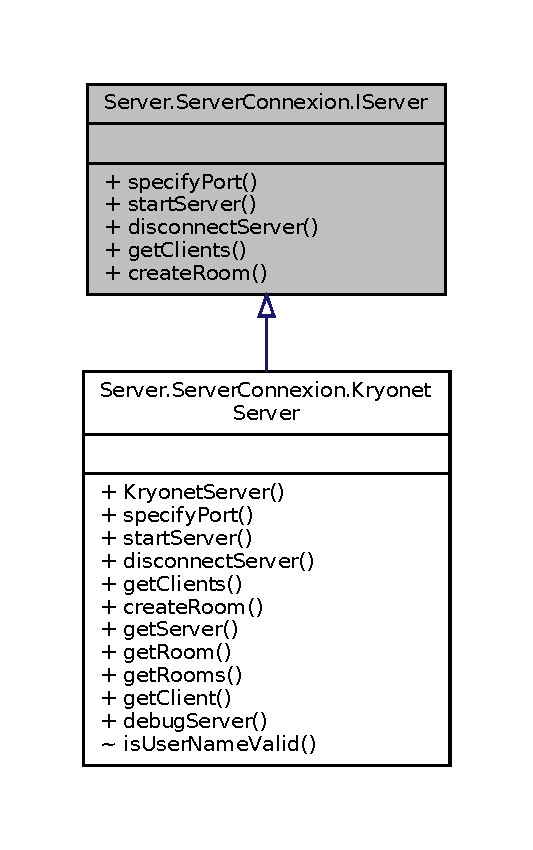
\includegraphics[width=256pt]{interfaceServer_1_1ServerConnexion_1_1IServer__inherit__graph}
\end{center}
\end{figure}


Collaboration diagram for Server.\+Server\+Connexion.\+I\+Server\+:
\nopagebreak
\begin{figure}[H]
\begin{center}
\leavevmode
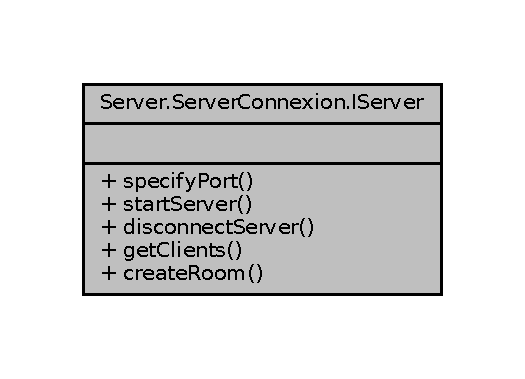
\includegraphics[width=252pt]{interfaceServer_1_1ServerConnexion_1_1IServer__coll__graph}
\end{center}
\end{figure}
\subsection*{Public Member Functions}
\begin{DoxyCompactItemize}
\item 
void \mbox{\hyperlink{interfaceServer_1_1ServerConnexion_1_1IServer_a708adb2b4f2312b4319496d92357bd0e}{specify\+Port}} (int port)
\item 
void \mbox{\hyperlink{interfaceServer_1_1ServerConnexion_1_1IServer_a13c33c54ae46ee73c99ae8b9a70b9397}{start\+Server}} ()
\item 
void \mbox{\hyperlink{interfaceServer_1_1ServerConnexion_1_1IServer_abad216cef2fde213cfe1e69f2be7b496}{disconnect\+Server}} ()
\item 
Concurrent\+Hash\+Map$<$ Integer, \mbox{\hyperlink{classServer_1_1ServerConnexion_1_1ClientInfos}{Client\+Infos}} $>$ \mbox{\hyperlink{interfaceServer_1_1ServerConnexion_1_1IServer_a0b71f139e86b01657d54b4be165d0c8d}{get\+Clients}} ()
\item 
void \mbox{\hyperlink{interfaceServer_1_1ServerConnexion_1_1IServer_a3b0485118add6720d6526c59605404d2}{create\+Room}} (\mbox{\hyperlink{classServer_1_1ServerConnexion_1_1ClientInfos}{Client\+Infos}} client)
\end{DoxyCompactItemize}


\subsection{Member Function Documentation}
\mbox{\Hypertarget{interfaceServer_1_1ServerConnexion_1_1IServer_a3b0485118add6720d6526c59605404d2}\label{interfaceServer_1_1ServerConnexion_1_1IServer_a3b0485118add6720d6526c59605404d2}} 
\index{Server\+::\+Server\+Connexion\+::\+I\+Server@{Server\+::\+Server\+Connexion\+::\+I\+Server}!create\+Room@{create\+Room}}
\index{create\+Room@{create\+Room}!Server\+::\+Server\+Connexion\+::\+I\+Server@{Server\+::\+Server\+Connexion\+::\+I\+Server}}
\subsubsection{\texorpdfstring{create\+Room()}{createRoom()}}
{\footnotesize\ttfamily void Server.\+Server\+Connexion.\+I\+Server.\+create\+Room (\begin{DoxyParamCaption}\item[{\mbox{\hyperlink{classServer_1_1ServerConnexion_1_1ClientInfos}{Client\+Infos}}}]{client }\end{DoxyParamCaption})}



Implemented in \mbox{\hyperlink{classServer_1_1ServerConnexion_1_1KryonetServer_ac594217673743346d963fa9e04f7a9dc}{Server.\+Server\+Connexion.\+Kryonet\+Server}}.

\mbox{\Hypertarget{interfaceServer_1_1ServerConnexion_1_1IServer_abad216cef2fde213cfe1e69f2be7b496}\label{interfaceServer_1_1ServerConnexion_1_1IServer_abad216cef2fde213cfe1e69f2be7b496}} 
\index{Server\+::\+Server\+Connexion\+::\+I\+Server@{Server\+::\+Server\+Connexion\+::\+I\+Server}!disconnect\+Server@{disconnect\+Server}}
\index{disconnect\+Server@{disconnect\+Server}!Server\+::\+Server\+Connexion\+::\+I\+Server@{Server\+::\+Server\+Connexion\+::\+I\+Server}}
\subsubsection{\texorpdfstring{disconnect\+Server()}{disconnectServer()}}
{\footnotesize\ttfamily void Server.\+Server\+Connexion.\+I\+Server.\+disconnect\+Server (\begin{DoxyParamCaption}{ }\end{DoxyParamCaption})}



Implemented in \mbox{\hyperlink{classServer_1_1ServerConnexion_1_1KryonetServer_a9ee03f7e9a0b2d685f4e70af32a8204e}{Server.\+Server\+Connexion.\+Kryonet\+Server}}.

\mbox{\Hypertarget{interfaceServer_1_1ServerConnexion_1_1IServer_a0b71f139e86b01657d54b4be165d0c8d}\label{interfaceServer_1_1ServerConnexion_1_1IServer_a0b71f139e86b01657d54b4be165d0c8d}} 
\index{Server\+::\+Server\+Connexion\+::\+I\+Server@{Server\+::\+Server\+Connexion\+::\+I\+Server}!get\+Clients@{get\+Clients}}
\index{get\+Clients@{get\+Clients}!Server\+::\+Server\+Connexion\+::\+I\+Server@{Server\+::\+Server\+Connexion\+::\+I\+Server}}
\subsubsection{\texorpdfstring{get\+Clients()}{getClients()}}
{\footnotesize\ttfamily Concurrent\+Hash\+Map$<$Integer, \mbox{\hyperlink{classServer_1_1ServerConnexion_1_1ClientInfos}{Client\+Infos}}$>$ Server.\+Server\+Connexion.\+I\+Server.\+get\+Clients (\begin{DoxyParamCaption}{ }\end{DoxyParamCaption})}



Implemented in \mbox{\hyperlink{classServer_1_1ServerConnexion_1_1KryonetServer_a49d513edab305edc72d56d173dd44ad3}{Server.\+Server\+Connexion.\+Kryonet\+Server}}.

\mbox{\Hypertarget{interfaceServer_1_1ServerConnexion_1_1IServer_a708adb2b4f2312b4319496d92357bd0e}\label{interfaceServer_1_1ServerConnexion_1_1IServer_a708adb2b4f2312b4319496d92357bd0e}} 
\index{Server\+::\+Server\+Connexion\+::\+I\+Server@{Server\+::\+Server\+Connexion\+::\+I\+Server}!specify\+Port@{specify\+Port}}
\index{specify\+Port@{specify\+Port}!Server\+::\+Server\+Connexion\+::\+I\+Server@{Server\+::\+Server\+Connexion\+::\+I\+Server}}
\subsubsection{\texorpdfstring{specify\+Port()}{specifyPort()}}
{\footnotesize\ttfamily void Server.\+Server\+Connexion.\+I\+Server.\+specify\+Port (\begin{DoxyParamCaption}\item[{int}]{port }\end{DoxyParamCaption})}



Implemented in \mbox{\hyperlink{classServer_1_1ServerConnexion_1_1KryonetServer_a5462e9f47eb97acd2d8353c825bf9f3b}{Server.\+Server\+Connexion.\+Kryonet\+Server}}.

\mbox{\Hypertarget{interfaceServer_1_1ServerConnexion_1_1IServer_a13c33c54ae46ee73c99ae8b9a70b9397}\label{interfaceServer_1_1ServerConnexion_1_1IServer_a13c33c54ae46ee73c99ae8b9a70b9397}} 
\index{Server\+::\+Server\+Connexion\+::\+I\+Server@{Server\+::\+Server\+Connexion\+::\+I\+Server}!start\+Server@{start\+Server}}
\index{start\+Server@{start\+Server}!Server\+::\+Server\+Connexion\+::\+I\+Server@{Server\+::\+Server\+Connexion\+::\+I\+Server}}
\subsubsection{\texorpdfstring{start\+Server()}{startServer()}}
{\footnotesize\ttfamily void Server.\+Server\+Connexion.\+I\+Server.\+start\+Server (\begin{DoxyParamCaption}{ }\end{DoxyParamCaption})}



Implemented in \mbox{\hyperlink{classServer_1_1ServerConnexion_1_1KryonetServer_a8bad9bf2baafbe83e2a6153c22b86bae}{Server.\+Server\+Connexion.\+Kryonet\+Server}}.



The documentation for this interface was generated from the following file\+:\begin{DoxyCompactItemize}
\item 
/home/tetard/\+Idea\+Projects/j\+Coinche/\+Java\+\_\+jcoinche\+\_\+2017/src/main/java/\+Server/\+Server\+Connexion/\mbox{\hyperlink{IServer_8java}{I\+Server.\+java}}\end{DoxyCompactItemize}

\hypertarget{classServer_1_1ServerConnexion_1_1KryonetServer}{}\section{Server.\+Server\+Connexion.\+Kryonet\+Server Class Reference}
\label{classServer_1_1ServerConnexion_1_1KryonetServer}\index{Server.\+Server\+Connexion.\+Kryonet\+Server@{Server.\+Server\+Connexion.\+Kryonet\+Server}}


Inheritance diagram for Server.\+Server\+Connexion.\+Kryonet\+Server\+:
\nopagebreak
\begin{figure}[H]
\begin{center}
\leavevmode
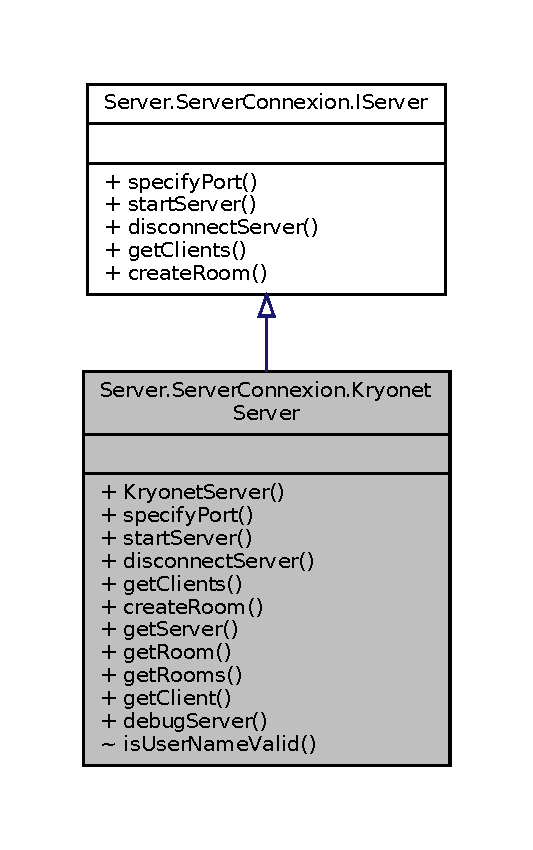
\includegraphics[width=256pt]{classServer_1_1ServerConnexion_1_1KryonetServer__inherit__graph}
\end{center}
\end{figure}


Collaboration diagram for Server.\+Server\+Connexion.\+Kryonet\+Server\+:
\nopagebreak
\begin{figure}[H]
\begin{center}
\leavevmode
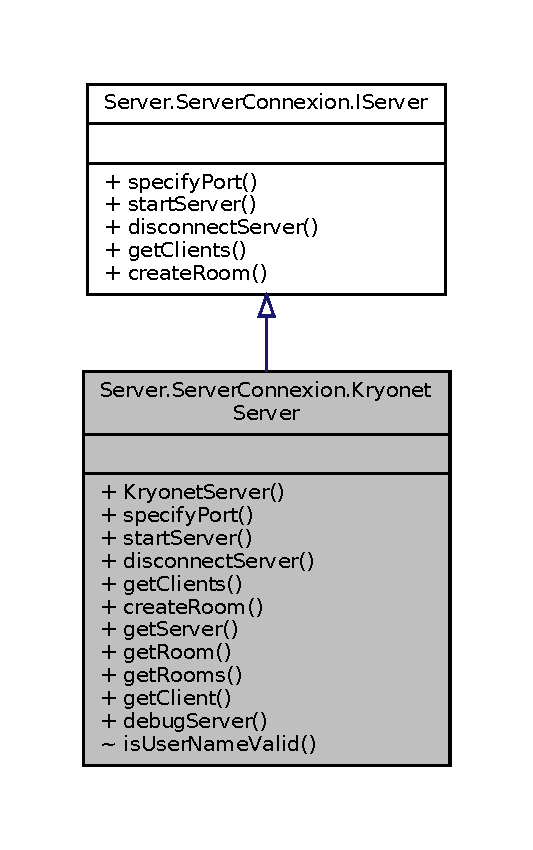
\includegraphics[width=256pt]{classServer_1_1ServerConnexion_1_1KryonetServer__coll__graph}
\end{center}
\end{figure}
\subsection*{Public Member Functions}
\begin{DoxyCompactItemize}
\item 
\mbox{\hyperlink{classServer_1_1ServerConnexion_1_1KryonetServer_a2882e79befe13a8c4d03316ee7e4629c}{Kryonet\+Server}} (int port)
\item 
void \mbox{\hyperlink{classServer_1_1ServerConnexion_1_1KryonetServer_a5462e9f47eb97acd2d8353c825bf9f3b}{specify\+Port}} (int port)
\item 
void \mbox{\hyperlink{classServer_1_1ServerConnexion_1_1KryonetServer_a8bad9bf2baafbe83e2a6153c22b86bae}{start\+Server}} ()
\item 
void \mbox{\hyperlink{classServer_1_1ServerConnexion_1_1KryonetServer_a9ee03f7e9a0b2d685f4e70af32a8204e}{disconnect\+Server}} ()
\item 
Concurrent\+Hash\+Map$<$ Integer, \mbox{\hyperlink{classServer_1_1ServerConnexion_1_1ClientInfos}{Client\+Infos}} $>$ \mbox{\hyperlink{classServer_1_1ServerConnexion_1_1KryonetServer_a49d513edab305edc72d56d173dd44ad3}{get\+Clients}} ()
\item 
void \mbox{\hyperlink{classServer_1_1ServerConnexion_1_1KryonetServer_ac594217673743346d963fa9e04f7a9dc}{create\+Room}} (\mbox{\hyperlink{classServer_1_1ServerConnexion_1_1ClientInfos}{Client\+Infos}} client)
\item 
Server \mbox{\hyperlink{classServer_1_1ServerConnexion_1_1KryonetServer_a2fc9a796907080bcbe65ec24304cca42}{get\+Server}} ()
\item 
\mbox{\hyperlink{classServer_1_1ServerConnexion_1_1Room}{Room}} \mbox{\hyperlink{classServer_1_1ServerConnexion_1_1KryonetServer_a4f294be7cbfd6a2c94191d3c488a9a12}{get\+Room}} (int room\+Id)
\item 
Concurrent\+Hash\+Map$<$ Integer, \mbox{\hyperlink{classServer_1_1ServerConnexion_1_1Room}{Room}} $>$ \mbox{\hyperlink{classServer_1_1ServerConnexion_1_1KryonetServer_ae0ff8432defb56e7801cac76e92c208d}{get\+Rooms}} ()
\item 
\mbox{\hyperlink{classServer_1_1ServerConnexion_1_1ClientInfos}{Client\+Infos}} \mbox{\hyperlink{classServer_1_1ServerConnexion_1_1KryonetServer_a0bc98a11530ff1d8734c29c7452b92f4}{get\+Client}} (int id)
\item 
void \mbox{\hyperlink{classServer_1_1ServerConnexion_1_1KryonetServer_acf5490a67284ed588a2167a12559ac5f}{debug\+Server}} ()  throws I\+O\+Exception 
\end{DoxyCompactItemize}


\subsection{Constructor \& Destructor Documentation}
\mbox{\Hypertarget{classServer_1_1ServerConnexion_1_1KryonetServer_a2882e79befe13a8c4d03316ee7e4629c}\label{classServer_1_1ServerConnexion_1_1KryonetServer_a2882e79befe13a8c4d03316ee7e4629c}} 
\index{Server\+::\+Server\+Connexion\+::\+Kryonet\+Server@{Server\+::\+Server\+Connexion\+::\+Kryonet\+Server}!Kryonet\+Server@{Kryonet\+Server}}
\index{Kryonet\+Server@{Kryonet\+Server}!Server\+::\+Server\+Connexion\+::\+Kryonet\+Server@{Server\+::\+Server\+Connexion\+::\+Kryonet\+Server}}
\subsubsection{\texorpdfstring{Kryonet\+Server()}{KryonetServer()}}
{\footnotesize\ttfamily Server.\+Server\+Connexion.\+Kryonet\+Server.\+Kryonet\+Server (\begin{DoxyParamCaption}\item[{int}]{port }\end{DoxyParamCaption})\hspace{0.3cm}{\ttfamily [inline]}}



\subsection{Member Function Documentation}
\mbox{\Hypertarget{classServer_1_1ServerConnexion_1_1KryonetServer_ac594217673743346d963fa9e04f7a9dc}\label{classServer_1_1ServerConnexion_1_1KryonetServer_ac594217673743346d963fa9e04f7a9dc}} 
\index{Server\+::\+Server\+Connexion\+::\+Kryonet\+Server@{Server\+::\+Server\+Connexion\+::\+Kryonet\+Server}!create\+Room@{create\+Room}}
\index{create\+Room@{create\+Room}!Server\+::\+Server\+Connexion\+::\+Kryonet\+Server@{Server\+::\+Server\+Connexion\+::\+Kryonet\+Server}}
\subsubsection{\texorpdfstring{create\+Room()}{createRoom()}}
{\footnotesize\ttfamily void Server.\+Server\+Connexion.\+Kryonet\+Server.\+create\+Room (\begin{DoxyParamCaption}\item[{\mbox{\hyperlink{classServer_1_1ServerConnexion_1_1ClientInfos}{Client\+Infos}}}]{client }\end{DoxyParamCaption})\hspace{0.3cm}{\ttfamily [inline]}}



Implements \mbox{\hyperlink{interfaceServer_1_1ServerConnexion_1_1IServer_a3b0485118add6720d6526c59605404d2}{Server.\+Server\+Connexion.\+I\+Server}}.

\mbox{\Hypertarget{classServer_1_1ServerConnexion_1_1KryonetServer_acf5490a67284ed588a2167a12559ac5f}\label{classServer_1_1ServerConnexion_1_1KryonetServer_acf5490a67284ed588a2167a12559ac5f}} 
\index{Server\+::\+Server\+Connexion\+::\+Kryonet\+Server@{Server\+::\+Server\+Connexion\+::\+Kryonet\+Server}!debug\+Server@{debug\+Server}}
\index{debug\+Server@{debug\+Server}!Server\+::\+Server\+Connexion\+::\+Kryonet\+Server@{Server\+::\+Server\+Connexion\+::\+Kryonet\+Server}}
\subsubsection{\texorpdfstring{debug\+Server()}{debugServer()}}
{\footnotesize\ttfamily void Server.\+Server\+Connexion.\+Kryonet\+Server.\+debug\+Server (\begin{DoxyParamCaption}{ }\end{DoxyParamCaption}) throws I\+O\+Exception\hspace{0.3cm}{\ttfamily [inline]}}

\mbox{\Hypertarget{classServer_1_1ServerConnexion_1_1KryonetServer_a9ee03f7e9a0b2d685f4e70af32a8204e}\label{classServer_1_1ServerConnexion_1_1KryonetServer_a9ee03f7e9a0b2d685f4e70af32a8204e}} 
\index{Server\+::\+Server\+Connexion\+::\+Kryonet\+Server@{Server\+::\+Server\+Connexion\+::\+Kryonet\+Server}!disconnect\+Server@{disconnect\+Server}}
\index{disconnect\+Server@{disconnect\+Server}!Server\+::\+Server\+Connexion\+::\+Kryonet\+Server@{Server\+::\+Server\+Connexion\+::\+Kryonet\+Server}}
\subsubsection{\texorpdfstring{disconnect\+Server()}{disconnectServer()}}
{\footnotesize\ttfamily void Server.\+Server\+Connexion.\+Kryonet\+Server.\+disconnect\+Server (\begin{DoxyParamCaption}{ }\end{DoxyParamCaption})\hspace{0.3cm}{\ttfamily [inline]}}



Implements \mbox{\hyperlink{interfaceServer_1_1ServerConnexion_1_1IServer_abad216cef2fde213cfe1e69f2be7b496}{Server.\+Server\+Connexion.\+I\+Server}}.

\mbox{\Hypertarget{classServer_1_1ServerConnexion_1_1KryonetServer_a0bc98a11530ff1d8734c29c7452b92f4}\label{classServer_1_1ServerConnexion_1_1KryonetServer_a0bc98a11530ff1d8734c29c7452b92f4}} 
\index{Server\+::\+Server\+Connexion\+::\+Kryonet\+Server@{Server\+::\+Server\+Connexion\+::\+Kryonet\+Server}!get\+Client@{get\+Client}}
\index{get\+Client@{get\+Client}!Server\+::\+Server\+Connexion\+::\+Kryonet\+Server@{Server\+::\+Server\+Connexion\+::\+Kryonet\+Server}}
\subsubsection{\texorpdfstring{get\+Client()}{getClient()}}
{\footnotesize\ttfamily \mbox{\hyperlink{classServer_1_1ServerConnexion_1_1ClientInfos}{Client\+Infos}} Server.\+Server\+Connexion.\+Kryonet\+Server.\+get\+Client (\begin{DoxyParamCaption}\item[{int}]{id }\end{DoxyParamCaption})\hspace{0.3cm}{\ttfamily [inline]}}

\mbox{\Hypertarget{classServer_1_1ServerConnexion_1_1KryonetServer_a49d513edab305edc72d56d173dd44ad3}\label{classServer_1_1ServerConnexion_1_1KryonetServer_a49d513edab305edc72d56d173dd44ad3}} 
\index{Server\+::\+Server\+Connexion\+::\+Kryonet\+Server@{Server\+::\+Server\+Connexion\+::\+Kryonet\+Server}!get\+Clients@{get\+Clients}}
\index{get\+Clients@{get\+Clients}!Server\+::\+Server\+Connexion\+::\+Kryonet\+Server@{Server\+::\+Server\+Connexion\+::\+Kryonet\+Server}}
\subsubsection{\texorpdfstring{get\+Clients()}{getClients()}}
{\footnotesize\ttfamily Concurrent\+Hash\+Map$<$Integer, \mbox{\hyperlink{classServer_1_1ServerConnexion_1_1ClientInfos}{Client\+Infos}}$>$ Server.\+Server\+Connexion.\+Kryonet\+Server.\+get\+Clients (\begin{DoxyParamCaption}{ }\end{DoxyParamCaption})\hspace{0.3cm}{\ttfamily [inline]}}



Implements \mbox{\hyperlink{interfaceServer_1_1ServerConnexion_1_1IServer_a0b71f139e86b01657d54b4be165d0c8d}{Server.\+Server\+Connexion.\+I\+Server}}.

\mbox{\Hypertarget{classServer_1_1ServerConnexion_1_1KryonetServer_a4f294be7cbfd6a2c94191d3c488a9a12}\label{classServer_1_1ServerConnexion_1_1KryonetServer_a4f294be7cbfd6a2c94191d3c488a9a12}} 
\index{Server\+::\+Server\+Connexion\+::\+Kryonet\+Server@{Server\+::\+Server\+Connexion\+::\+Kryonet\+Server}!get\+Room@{get\+Room}}
\index{get\+Room@{get\+Room}!Server\+::\+Server\+Connexion\+::\+Kryonet\+Server@{Server\+::\+Server\+Connexion\+::\+Kryonet\+Server}}
\subsubsection{\texorpdfstring{get\+Room()}{getRoom()}}
{\footnotesize\ttfamily \mbox{\hyperlink{classServer_1_1ServerConnexion_1_1Room}{Room}} Server.\+Server\+Connexion.\+Kryonet\+Server.\+get\+Room (\begin{DoxyParamCaption}\item[{int}]{room\+Id }\end{DoxyParamCaption})\hspace{0.3cm}{\ttfamily [inline]}}

\mbox{\Hypertarget{classServer_1_1ServerConnexion_1_1KryonetServer_ae0ff8432defb56e7801cac76e92c208d}\label{classServer_1_1ServerConnexion_1_1KryonetServer_ae0ff8432defb56e7801cac76e92c208d}} 
\index{Server\+::\+Server\+Connexion\+::\+Kryonet\+Server@{Server\+::\+Server\+Connexion\+::\+Kryonet\+Server}!get\+Rooms@{get\+Rooms}}
\index{get\+Rooms@{get\+Rooms}!Server\+::\+Server\+Connexion\+::\+Kryonet\+Server@{Server\+::\+Server\+Connexion\+::\+Kryonet\+Server}}
\subsubsection{\texorpdfstring{get\+Rooms()}{getRooms()}}
{\footnotesize\ttfamily Concurrent\+Hash\+Map$<$Integer, \mbox{\hyperlink{classServer_1_1ServerConnexion_1_1Room}{Room}}$>$ Server.\+Server\+Connexion.\+Kryonet\+Server.\+get\+Rooms (\begin{DoxyParamCaption}{ }\end{DoxyParamCaption})\hspace{0.3cm}{\ttfamily [inline]}}

\mbox{\Hypertarget{classServer_1_1ServerConnexion_1_1KryonetServer_a2fc9a796907080bcbe65ec24304cca42}\label{classServer_1_1ServerConnexion_1_1KryonetServer_a2fc9a796907080bcbe65ec24304cca42}} 
\index{Server\+::\+Server\+Connexion\+::\+Kryonet\+Server@{Server\+::\+Server\+Connexion\+::\+Kryonet\+Server}!get\+Server@{get\+Server}}
\index{get\+Server@{get\+Server}!Server\+::\+Server\+Connexion\+::\+Kryonet\+Server@{Server\+::\+Server\+Connexion\+::\+Kryonet\+Server}}
\subsubsection{\texorpdfstring{get\+Server()}{getServer()}}
{\footnotesize\ttfamily Server Server.\+Server\+Connexion.\+Kryonet\+Server.\+get\+Server (\begin{DoxyParamCaption}{ }\end{DoxyParamCaption})\hspace{0.3cm}{\ttfamily [inline]}}

\mbox{\Hypertarget{classServer_1_1ServerConnexion_1_1KryonetServer_a5462e9f47eb97acd2d8353c825bf9f3b}\label{classServer_1_1ServerConnexion_1_1KryonetServer_a5462e9f47eb97acd2d8353c825bf9f3b}} 
\index{Server\+::\+Server\+Connexion\+::\+Kryonet\+Server@{Server\+::\+Server\+Connexion\+::\+Kryonet\+Server}!specify\+Port@{specify\+Port}}
\index{specify\+Port@{specify\+Port}!Server\+::\+Server\+Connexion\+::\+Kryonet\+Server@{Server\+::\+Server\+Connexion\+::\+Kryonet\+Server}}
\subsubsection{\texorpdfstring{specify\+Port()}{specifyPort()}}
{\footnotesize\ttfamily void Server.\+Server\+Connexion.\+Kryonet\+Server.\+specify\+Port (\begin{DoxyParamCaption}\item[{int}]{port }\end{DoxyParamCaption})\hspace{0.3cm}{\ttfamily [inline]}}



Implements \mbox{\hyperlink{interfaceServer_1_1ServerConnexion_1_1IServer_a708adb2b4f2312b4319496d92357bd0e}{Server.\+Server\+Connexion.\+I\+Server}}.

\mbox{\Hypertarget{classServer_1_1ServerConnexion_1_1KryonetServer_a8bad9bf2baafbe83e2a6153c22b86bae}\label{classServer_1_1ServerConnexion_1_1KryonetServer_a8bad9bf2baafbe83e2a6153c22b86bae}} 
\index{Server\+::\+Server\+Connexion\+::\+Kryonet\+Server@{Server\+::\+Server\+Connexion\+::\+Kryonet\+Server}!start\+Server@{start\+Server}}
\index{start\+Server@{start\+Server}!Server\+::\+Server\+Connexion\+::\+Kryonet\+Server@{Server\+::\+Server\+Connexion\+::\+Kryonet\+Server}}
\subsubsection{\texorpdfstring{start\+Server()}{startServer()}}
{\footnotesize\ttfamily void Server.\+Server\+Connexion.\+Kryonet\+Server.\+start\+Server (\begin{DoxyParamCaption}{ }\end{DoxyParamCaption})\hspace{0.3cm}{\ttfamily [inline]}}



Implements \mbox{\hyperlink{interfaceServer_1_1ServerConnexion_1_1IServer_a13c33c54ae46ee73c99ae8b9a70b9397}{Server.\+Server\+Connexion.\+I\+Server}}.



The documentation for this class was generated from the following file\+:\begin{DoxyCompactItemize}
\item 
/home/tetard/\+Idea\+Projects/j\+Coinche/\+Java\+\_\+jcoinche\+\_\+2017/src/main/java/\+Server/\+Server\+Connexion/\mbox{\hyperlink{KryonetServer_8java}{Kryonet\+Server.\+java}}\end{DoxyCompactItemize}

\hypertarget{classCommon_1_1KryoTool}{}\section{Common.\+Kryo\+Tool Class Reference}
\label{classCommon_1_1KryoTool}\index{Common.\+Kryo\+Tool@{Common.\+Kryo\+Tool}}


Collaboration diagram for Common.\+Kryo\+Tool\+:
\nopagebreak
\begin{figure}[H]
\begin{center}
\leavevmode
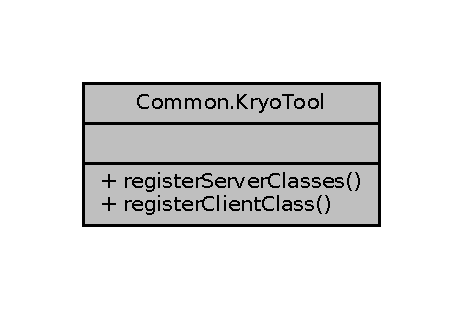
\includegraphics[width=222pt]{classCommon_1_1KryoTool__coll__graph}
\end{center}
\end{figure}
\subsection*{Static Public Member Functions}
\begin{DoxyCompactItemize}
\item 
static void \mbox{\hyperlink{classCommon_1_1KryoTool_a263006a45f41c011a3ad7dfb0086f551}{register\+Server\+Classes}} (Server server)
\item 
static void \mbox{\hyperlink{classCommon_1_1KryoTool_ab2aa3283b39bc6f71f770f51e76d8246}{register\+Client\+Class}} (Client client)
\end{DoxyCompactItemize}


\subsection{Member Function Documentation}
\mbox{\Hypertarget{classCommon_1_1KryoTool_ab2aa3283b39bc6f71f770f51e76d8246}\label{classCommon_1_1KryoTool_ab2aa3283b39bc6f71f770f51e76d8246}} 
\index{Common\+::\+Kryo\+Tool@{Common\+::\+Kryo\+Tool}!register\+Client\+Class@{register\+Client\+Class}}
\index{register\+Client\+Class@{register\+Client\+Class}!Common\+::\+Kryo\+Tool@{Common\+::\+Kryo\+Tool}}
\subsubsection{\texorpdfstring{register\+Client\+Class()}{registerClientClass()}}
{\footnotesize\ttfamily static void Common.\+Kryo\+Tool.\+register\+Client\+Class (\begin{DoxyParamCaption}\item[{Client}]{client }\end{DoxyParamCaption})\hspace{0.3cm}{\ttfamily [inline]}, {\ttfamily [static]}}

\mbox{\Hypertarget{classCommon_1_1KryoTool_a263006a45f41c011a3ad7dfb0086f551}\label{classCommon_1_1KryoTool_a263006a45f41c011a3ad7dfb0086f551}} 
\index{Common\+::\+Kryo\+Tool@{Common\+::\+Kryo\+Tool}!register\+Server\+Classes@{register\+Server\+Classes}}
\index{register\+Server\+Classes@{register\+Server\+Classes}!Common\+::\+Kryo\+Tool@{Common\+::\+Kryo\+Tool}}
\subsubsection{\texorpdfstring{register\+Server\+Classes()}{registerServerClasses()}}
{\footnotesize\ttfamily static void Common.\+Kryo\+Tool.\+register\+Server\+Classes (\begin{DoxyParamCaption}\item[{Server}]{server }\end{DoxyParamCaption})\hspace{0.3cm}{\ttfamily [inline]}, {\ttfamily [static]}}



The documentation for this class was generated from the following file\+:\begin{DoxyCompactItemize}
\item 
/home/tetard/\+Idea\+Projects/j\+Coinche/\+Java\+\_\+jcoinche\+\_\+2017/src/main/java/\+Common/\mbox{\hyperlink{KryoTool_8java}{Kryo\+Tool.\+java}}\end{DoxyCompactItemize}

\hypertarget{classClient_1_1Main}{}\section{Client.\+Main Class Reference}
\label{classClient_1_1Main}\index{Client.\+Main@{Client.\+Main}}


Collaboration diagram for Client.\+Main\+:
\nopagebreak
\begin{figure}[H]
\begin{center}
\leavevmode
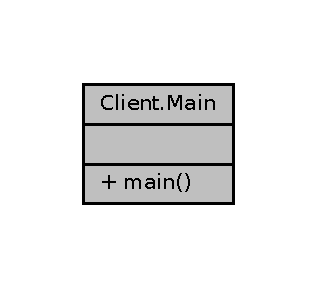
\includegraphics[width=152pt]{classClient_1_1Main__coll__graph}
\end{center}
\end{figure}
\subsection*{Static Public Member Functions}
\begin{DoxyCompactItemize}
\item 
static void \mbox{\hyperlink{classClient_1_1Main_aa2aae7f6458f541210f294b25fb7ef02}{main}} (String\mbox{[}$\,$\mbox{]} args)  throws I\+O\+Exception, Interrupted\+Exception 
\end{DoxyCompactItemize}


\subsection{Member Function Documentation}
\mbox{\Hypertarget{classClient_1_1Main_aa2aae7f6458f541210f294b25fb7ef02}\label{classClient_1_1Main_aa2aae7f6458f541210f294b25fb7ef02}} 
\index{Client\+::\+Main@{Client\+::\+Main}!main@{main}}
\index{main@{main}!Client\+::\+Main@{Client\+::\+Main}}
\subsubsection{\texorpdfstring{main()}{main()}}
{\footnotesize\ttfamily static void Client.\+Main.\+main (\begin{DoxyParamCaption}\item[{String \mbox{[}$\,$\mbox{]}}]{args }\end{DoxyParamCaption}) throws I\+O\+Exception, Interrupted\+Exception\hspace{0.3cm}{\ttfamily [inline]}, {\ttfamily [static]}}



The documentation for this class was generated from the following file\+:\begin{DoxyCompactItemize}
\item 
/home/tetard/\+Idea\+Projects/j\+Coinche/\+Java\+\_\+jcoinche\+\_\+2017/src/main/java/\+Client/\mbox{\hyperlink{Client_2Main_8java}{Main.\+java}}\end{DoxyCompactItemize}

\hypertarget{classServer_1_1Main}{}\section{Server.\+Main Class Reference}
\label{classServer_1_1Main}\index{Server.\+Main@{Server.\+Main}}


Collaboration diagram for Server.\+Main\+:
\nopagebreak
\begin{figure}[H]
\begin{center}
\leavevmode
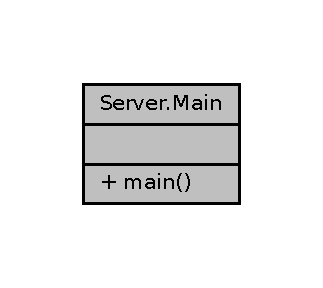
\includegraphics[width=155pt]{classServer_1_1Main__coll__graph}
\end{center}
\end{figure}
\subsection*{Static Public Member Functions}
\begin{DoxyCompactItemize}
\item 
static void \mbox{\hyperlink{classServer_1_1Main_a76af90a600f09ced690adf36a6a1dfce}{main}} (String\mbox{[}$\,$\mbox{]} args)  throws Interrupted\+Exception, I\+O\+Exception 
\end{DoxyCompactItemize}


\subsection{Member Function Documentation}
\mbox{\Hypertarget{classServer_1_1Main_a76af90a600f09ced690adf36a6a1dfce}\label{classServer_1_1Main_a76af90a600f09ced690adf36a6a1dfce}} 
\index{Server\+::\+Main@{Server\+::\+Main}!main@{main}}
\index{main@{main}!Server\+::\+Main@{Server\+::\+Main}}
\subsubsection{\texorpdfstring{main()}{main()}}
{\footnotesize\ttfamily static void Server.\+Main.\+main (\begin{DoxyParamCaption}\item[{String \mbox{[}$\,$\mbox{]}}]{args }\end{DoxyParamCaption}) throws Interrupted\+Exception, I\+O\+Exception\hspace{0.3cm}{\ttfamily [inline]}, {\ttfamily [static]}}



The documentation for this class was generated from the following file\+:\begin{DoxyCompactItemize}
\item 
/home/tetard/\+Idea\+Projects/j\+Coinche/\+Java\+\_\+jcoinche\+\_\+2017/src/main/java/\+Server/\mbox{\hyperlink{Server_2Main_8java}{Main.\+java}}\end{DoxyCompactItemize}

\hypertarget{classClient_1_1Model_1_1Other}{}\section{Client.\+Model.\+Other Class Reference}
\label{classClient_1_1Model_1_1Other}\index{Client.\+Model.\+Other@{Client.\+Model.\+Other}}


Collaboration diagram for Client.\+Model.\+Other\+:
\nopagebreak
\begin{figure}[H]
\begin{center}
\leavevmode
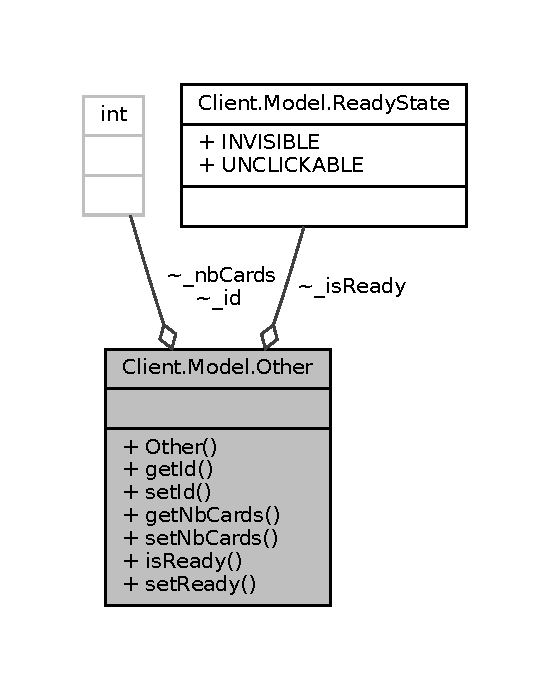
\includegraphics[width=264pt]{classClient_1_1Model_1_1Other__coll__graph}
\end{center}
\end{figure}
\subsection*{Public Member Functions}
\begin{DoxyCompactItemize}
\item 
\mbox{\hyperlink{classClient_1_1Model_1_1Other_a90aa8eae420b2d79005975df8ac0b120}{Other}} (int id)
\item 
int \mbox{\hyperlink{classClient_1_1Model_1_1Other_afa3b96824bac044a570833d3e829e14e}{get\+Id}} ()
\item 
void \mbox{\hyperlink{classClient_1_1Model_1_1Other_ab6220f1b2ff6b125d99d58deb84e0079}{set\+Id}} (int id)
\item 
int \mbox{\hyperlink{classClient_1_1Model_1_1Other_ae0917c370d73e73fc2e4ebfa9049e952}{get\+Nb\+Cards}} ()
\item 
void \mbox{\hyperlink{classClient_1_1Model_1_1Other_a4cfa780b4d0bdb50a553687ba49cd7f8}{set\+Nb\+Cards}} (int nb\+Cards)
\item 
\mbox{\hyperlink{enumClient_1_1Model_1_1ReadyState}{Ready\+State}} \mbox{\hyperlink{classClient_1_1Model_1_1Other_a2441862fc21c750ebaf88b87af040d14}{is\+Ready}} ()
\item 
void \mbox{\hyperlink{classClient_1_1Model_1_1Other_a46277632c220da183bbcde7e27688456}{set\+Ready}} (\mbox{\hyperlink{enumClient_1_1Model_1_1ReadyState}{Ready\+State}} ready)
\end{DoxyCompactItemize}


\subsection{Constructor \& Destructor Documentation}
\mbox{\Hypertarget{classClient_1_1Model_1_1Other_a90aa8eae420b2d79005975df8ac0b120}\label{classClient_1_1Model_1_1Other_a90aa8eae420b2d79005975df8ac0b120}} 
\index{Client\+::\+Model\+::\+Other@{Client\+::\+Model\+::\+Other}!Other@{Other}}
\index{Other@{Other}!Client\+::\+Model\+::\+Other@{Client\+::\+Model\+::\+Other}}
\subsubsection{\texorpdfstring{Other()}{Other()}}
{\footnotesize\ttfamily Client.\+Model.\+Other.\+Other (\begin{DoxyParamCaption}\item[{int}]{id }\end{DoxyParamCaption})\hspace{0.3cm}{\ttfamily [inline]}}



\subsection{Member Function Documentation}
\mbox{\Hypertarget{classClient_1_1Model_1_1Other_afa3b96824bac044a570833d3e829e14e}\label{classClient_1_1Model_1_1Other_afa3b96824bac044a570833d3e829e14e}} 
\index{Client\+::\+Model\+::\+Other@{Client\+::\+Model\+::\+Other}!get\+Id@{get\+Id}}
\index{get\+Id@{get\+Id}!Client\+::\+Model\+::\+Other@{Client\+::\+Model\+::\+Other}}
\subsubsection{\texorpdfstring{get\+Id()}{getId()}}
{\footnotesize\ttfamily int Client.\+Model.\+Other.\+get\+Id (\begin{DoxyParamCaption}{ }\end{DoxyParamCaption})\hspace{0.3cm}{\ttfamily [inline]}}

\mbox{\Hypertarget{classClient_1_1Model_1_1Other_ae0917c370d73e73fc2e4ebfa9049e952}\label{classClient_1_1Model_1_1Other_ae0917c370d73e73fc2e4ebfa9049e952}} 
\index{Client\+::\+Model\+::\+Other@{Client\+::\+Model\+::\+Other}!get\+Nb\+Cards@{get\+Nb\+Cards}}
\index{get\+Nb\+Cards@{get\+Nb\+Cards}!Client\+::\+Model\+::\+Other@{Client\+::\+Model\+::\+Other}}
\subsubsection{\texorpdfstring{get\+Nb\+Cards()}{getNbCards()}}
{\footnotesize\ttfamily int Client.\+Model.\+Other.\+get\+Nb\+Cards (\begin{DoxyParamCaption}{ }\end{DoxyParamCaption})\hspace{0.3cm}{\ttfamily [inline]}}

\mbox{\Hypertarget{classClient_1_1Model_1_1Other_a2441862fc21c750ebaf88b87af040d14}\label{classClient_1_1Model_1_1Other_a2441862fc21c750ebaf88b87af040d14}} 
\index{Client\+::\+Model\+::\+Other@{Client\+::\+Model\+::\+Other}!is\+Ready@{is\+Ready}}
\index{is\+Ready@{is\+Ready}!Client\+::\+Model\+::\+Other@{Client\+::\+Model\+::\+Other}}
\subsubsection{\texorpdfstring{is\+Ready()}{isReady()}}
{\footnotesize\ttfamily \mbox{\hyperlink{enumClient_1_1Model_1_1ReadyState}{Ready\+State}} Client.\+Model.\+Other.\+is\+Ready (\begin{DoxyParamCaption}{ }\end{DoxyParamCaption})\hspace{0.3cm}{\ttfamily [inline]}}

\mbox{\Hypertarget{classClient_1_1Model_1_1Other_ab6220f1b2ff6b125d99d58deb84e0079}\label{classClient_1_1Model_1_1Other_ab6220f1b2ff6b125d99d58deb84e0079}} 
\index{Client\+::\+Model\+::\+Other@{Client\+::\+Model\+::\+Other}!set\+Id@{set\+Id}}
\index{set\+Id@{set\+Id}!Client\+::\+Model\+::\+Other@{Client\+::\+Model\+::\+Other}}
\subsubsection{\texorpdfstring{set\+Id()}{setId()}}
{\footnotesize\ttfamily void Client.\+Model.\+Other.\+set\+Id (\begin{DoxyParamCaption}\item[{int}]{id }\end{DoxyParamCaption})\hspace{0.3cm}{\ttfamily [inline]}}

\mbox{\Hypertarget{classClient_1_1Model_1_1Other_a4cfa780b4d0bdb50a553687ba49cd7f8}\label{classClient_1_1Model_1_1Other_a4cfa780b4d0bdb50a553687ba49cd7f8}} 
\index{Client\+::\+Model\+::\+Other@{Client\+::\+Model\+::\+Other}!set\+Nb\+Cards@{set\+Nb\+Cards}}
\index{set\+Nb\+Cards@{set\+Nb\+Cards}!Client\+::\+Model\+::\+Other@{Client\+::\+Model\+::\+Other}}
\subsubsection{\texorpdfstring{set\+Nb\+Cards()}{setNbCards()}}
{\footnotesize\ttfamily void Client.\+Model.\+Other.\+set\+Nb\+Cards (\begin{DoxyParamCaption}\item[{int}]{nb\+Cards }\end{DoxyParamCaption})\hspace{0.3cm}{\ttfamily [inline]}}

\mbox{\Hypertarget{classClient_1_1Model_1_1Other_a46277632c220da183bbcde7e27688456}\label{classClient_1_1Model_1_1Other_a46277632c220da183bbcde7e27688456}} 
\index{Client\+::\+Model\+::\+Other@{Client\+::\+Model\+::\+Other}!set\+Ready@{set\+Ready}}
\index{set\+Ready@{set\+Ready}!Client\+::\+Model\+::\+Other@{Client\+::\+Model\+::\+Other}}
\subsubsection{\texorpdfstring{set\+Ready()}{setReady()}}
{\footnotesize\ttfamily void Client.\+Model.\+Other.\+set\+Ready (\begin{DoxyParamCaption}\item[{\mbox{\hyperlink{enumClient_1_1Model_1_1ReadyState}{Ready\+State}}}]{ready }\end{DoxyParamCaption})\hspace{0.3cm}{\ttfamily [inline]}}



The documentation for this class was generated from the following file\+:\begin{DoxyCompactItemize}
\item 
/home/tetard/\+Idea\+Projects/j\+Coinche/\+Java\+\_\+jcoinche\+\_\+2017/src/main/java/\+Client/\+Model/\mbox{\hyperlink{Other_8java}{Other.\+java}}\end{DoxyCompactItemize}

\hypertarget{classCommon_1_1PartyCancelled}{}\section{Common.\+Party\+Cancelled Class Reference}
\label{classCommon_1_1PartyCancelled}\index{Common.\+Party\+Cancelled@{Common.\+Party\+Cancelled}}


Collaboration diagram for Common.\+Party\+Cancelled\+:
\nopagebreak
\begin{figure}[H]
\begin{center}
\leavevmode
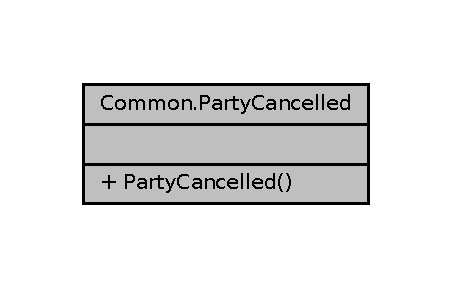
\includegraphics[width=217pt]{classCommon_1_1PartyCancelled__coll__graph}
\end{center}
\end{figure}
\subsection*{Public Member Functions}
\begin{DoxyCompactItemize}
\item 
\mbox{\hyperlink{classCommon_1_1PartyCancelled_a02a33bea3c55eac9683b6dc1f5f380b4}{Party\+Cancelled}} ()
\end{DoxyCompactItemize}


\subsection{Constructor \& Destructor Documentation}
\mbox{\Hypertarget{classCommon_1_1PartyCancelled_a02a33bea3c55eac9683b6dc1f5f380b4}\label{classCommon_1_1PartyCancelled_a02a33bea3c55eac9683b6dc1f5f380b4}} 
\index{Common\+::\+Party\+Cancelled@{Common\+::\+Party\+Cancelled}!Party\+Cancelled@{Party\+Cancelled}}
\index{Party\+Cancelled@{Party\+Cancelled}!Common\+::\+Party\+Cancelled@{Common\+::\+Party\+Cancelled}}
\subsubsection{\texorpdfstring{Party\+Cancelled()}{PartyCancelled()}}
{\footnotesize\ttfamily Common.\+Party\+Cancelled.\+Party\+Cancelled (\begin{DoxyParamCaption}{ }\end{DoxyParamCaption})\hspace{0.3cm}{\ttfamily [inline]}}



The documentation for this class was generated from the following file\+:\begin{DoxyCompactItemize}
\item 
/home/tetard/\+Idea\+Projects/j\+Coinche/\+Java\+\_\+jcoinche\+\_\+2017/src/main/java/\+Common/\mbox{\hyperlink{PartyCancelled_8java}{Party\+Cancelled.\+java}}\end{DoxyCompactItemize}

\hypertarget{classCommon_1_1Player}{}\section{Common.\+Player Class Reference}
\label{classCommon_1_1Player}\index{Common.\+Player@{Common.\+Player}}


Collaboration diagram for Common.\+Player\+:
\nopagebreak
\begin{figure}[H]
\begin{center}
\leavevmode
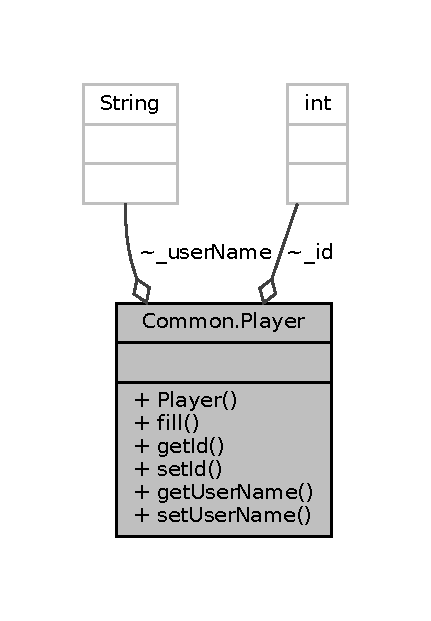
\includegraphics[width=207pt]{classCommon_1_1Player__coll__graph}
\end{center}
\end{figure}
\subsection*{Public Member Functions}
\begin{DoxyCompactItemize}
\item 
\mbox{\hyperlink{classCommon_1_1Player_a41dd3f4886d9e2a500c11be33ee73037}{Player}} ()
\item 
\mbox{\hyperlink{classCommon_1_1Player}{Player}} \mbox{\hyperlink{classCommon_1_1Player_a210c67d034b0b8ed9ead15c78a160829}{fill}} (int id, String user\+Name)
\item 
int \mbox{\hyperlink{classCommon_1_1Player_a713d057ef14b76119f3dfadc144ba150}{get\+Id}} ()
\item 
void \mbox{\hyperlink{classCommon_1_1Player_a400188d44456475d7864021917d9fe88}{set\+Id}} (int id)
\item 
String \mbox{\hyperlink{classCommon_1_1Player_a0b71351bbbea5a4624cafc7a9046b227}{get\+User\+Name}} ()
\item 
void \mbox{\hyperlink{classCommon_1_1Player_a89374a2bf8698d365493343ed49c7750}{set\+User\+Name}} (String user\+Name)
\end{DoxyCompactItemize}


\subsection{Constructor \& Destructor Documentation}
\mbox{\Hypertarget{classCommon_1_1Player_a41dd3f4886d9e2a500c11be33ee73037}\label{classCommon_1_1Player_a41dd3f4886d9e2a500c11be33ee73037}} 
\index{Common\+::\+Player@{Common\+::\+Player}!Player@{Player}}
\index{Player@{Player}!Common\+::\+Player@{Common\+::\+Player}}
\subsubsection{\texorpdfstring{Player()}{Player()}}
{\footnotesize\ttfamily Common.\+Player.\+Player (\begin{DoxyParamCaption}{ }\end{DoxyParamCaption})\hspace{0.3cm}{\ttfamily [inline]}}



\subsection{Member Function Documentation}
\mbox{\Hypertarget{classCommon_1_1Player_a210c67d034b0b8ed9ead15c78a160829}\label{classCommon_1_1Player_a210c67d034b0b8ed9ead15c78a160829}} 
\index{Common\+::\+Player@{Common\+::\+Player}!fill@{fill}}
\index{fill@{fill}!Common\+::\+Player@{Common\+::\+Player}}
\subsubsection{\texorpdfstring{fill()}{fill()}}
{\footnotesize\ttfamily \mbox{\hyperlink{classCommon_1_1Player}{Player}} Common.\+Player.\+fill (\begin{DoxyParamCaption}\item[{int}]{id,  }\item[{String}]{user\+Name }\end{DoxyParamCaption})\hspace{0.3cm}{\ttfamily [inline]}}

\mbox{\Hypertarget{classCommon_1_1Player_a713d057ef14b76119f3dfadc144ba150}\label{classCommon_1_1Player_a713d057ef14b76119f3dfadc144ba150}} 
\index{Common\+::\+Player@{Common\+::\+Player}!get\+Id@{get\+Id}}
\index{get\+Id@{get\+Id}!Common\+::\+Player@{Common\+::\+Player}}
\subsubsection{\texorpdfstring{get\+Id()}{getId()}}
{\footnotesize\ttfamily int Common.\+Player.\+get\+Id (\begin{DoxyParamCaption}{ }\end{DoxyParamCaption})\hspace{0.3cm}{\ttfamily [inline]}}

\mbox{\Hypertarget{classCommon_1_1Player_a0b71351bbbea5a4624cafc7a9046b227}\label{classCommon_1_1Player_a0b71351bbbea5a4624cafc7a9046b227}} 
\index{Common\+::\+Player@{Common\+::\+Player}!get\+User\+Name@{get\+User\+Name}}
\index{get\+User\+Name@{get\+User\+Name}!Common\+::\+Player@{Common\+::\+Player}}
\subsubsection{\texorpdfstring{get\+User\+Name()}{getUserName()}}
{\footnotesize\ttfamily String Common.\+Player.\+get\+User\+Name (\begin{DoxyParamCaption}{ }\end{DoxyParamCaption})\hspace{0.3cm}{\ttfamily [inline]}}

\mbox{\Hypertarget{classCommon_1_1Player_a400188d44456475d7864021917d9fe88}\label{classCommon_1_1Player_a400188d44456475d7864021917d9fe88}} 
\index{Common\+::\+Player@{Common\+::\+Player}!set\+Id@{set\+Id}}
\index{set\+Id@{set\+Id}!Common\+::\+Player@{Common\+::\+Player}}
\subsubsection{\texorpdfstring{set\+Id()}{setId()}}
{\footnotesize\ttfamily void Common.\+Player.\+set\+Id (\begin{DoxyParamCaption}\item[{int}]{id }\end{DoxyParamCaption})\hspace{0.3cm}{\ttfamily [inline]}}

\mbox{\Hypertarget{classCommon_1_1Player_a89374a2bf8698d365493343ed49c7750}\label{classCommon_1_1Player_a89374a2bf8698d365493343ed49c7750}} 
\index{Common\+::\+Player@{Common\+::\+Player}!set\+User\+Name@{set\+User\+Name}}
\index{set\+User\+Name@{set\+User\+Name}!Common\+::\+Player@{Common\+::\+Player}}
\subsubsection{\texorpdfstring{set\+User\+Name()}{setUserName()}}
{\footnotesize\ttfamily void Common.\+Player.\+set\+User\+Name (\begin{DoxyParamCaption}\item[{String}]{user\+Name }\end{DoxyParamCaption})\hspace{0.3cm}{\ttfamily [inline]}}



The documentation for this class was generated from the following file\+:\begin{DoxyCompactItemize}
\item 
/home/tetard/\+Idea\+Projects/j\+Coinche/\+Java\+\_\+jcoinche\+\_\+2017/src/main/java/\+Common/\mbox{\hyperlink{Player_8java}{Player.\+java}}\end{DoxyCompactItemize}

\hypertarget{classCommon_1_1PlayerCallResponse}{}\section{Common.\+Player\+Call\+Response Class Reference}
\label{classCommon_1_1PlayerCallResponse}\index{Common.\+Player\+Call\+Response@{Common.\+Player\+Call\+Response}}


Collaboration diagram for Common.\+Player\+Call\+Response\+:
\nopagebreak
\begin{figure}[H]
\begin{center}
\leavevmode
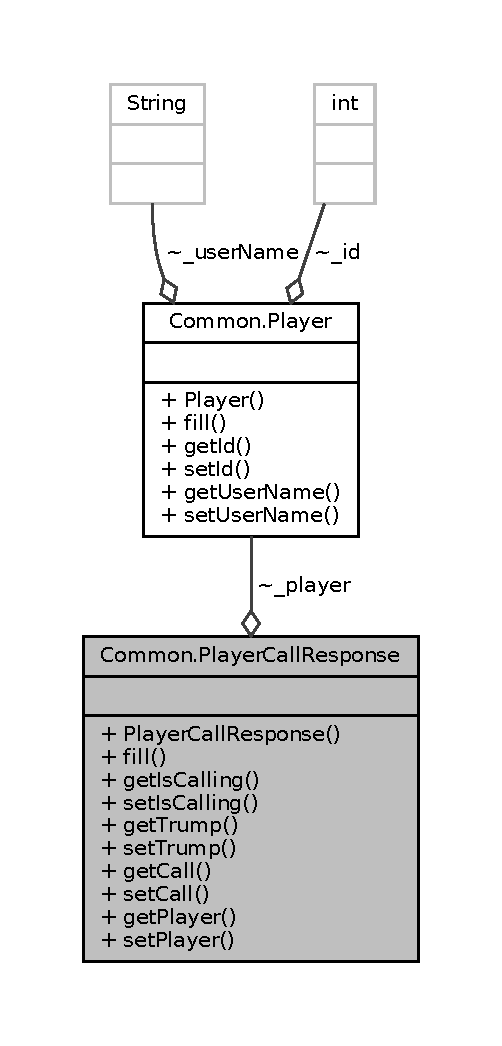
\includegraphics[width=241pt]{classCommon_1_1PlayerCallResponse__coll__graph}
\end{center}
\end{figure}
\subsection*{Public Member Functions}
\begin{DoxyCompactItemize}
\item 
\mbox{\hyperlink{classCommon_1_1PlayerCallResponse_aa05af4c1843c3d7bf51ad6bdf0aad835}{Player\+Call\+Response}} ()
\item 
\mbox{\hyperlink{classCommon_1_1PlayerCallResponse}{Player\+Call\+Response}} \mbox{\hyperlink{classCommon_1_1PlayerCallResponse_a8273a7383a1b5c1bc459a1316b179709}{fill}} (\mbox{\hyperlink{classCommon_1_1Player}{Player}} player, boolean is\+Calling, \mbox{\hyperlink{enumCommon_1_1Trump}{Trump}} trump, int call)
\item 
boolean \mbox{\hyperlink{classCommon_1_1PlayerCallResponse_a902c88481b0437ae506fc8433714fe1f}{get\+Is\+Calling}} ()
\item 
void \mbox{\hyperlink{classCommon_1_1PlayerCallResponse_a4ae271562532326e9a46aaa44457c900}{set\+Is\+Calling}} (boolean \+\_\+is\+Calling)
\item 
\mbox{\hyperlink{enumCommon_1_1Trump}{Trump}} \mbox{\hyperlink{classCommon_1_1PlayerCallResponse_a7148bd90f3c12c061ca28a8adf168c48}{get\+Trump}} ()
\item 
void \mbox{\hyperlink{classCommon_1_1PlayerCallResponse_aa34a0f910c4f9a03e9fe89b3777d74c0}{set\+Trump}} (\mbox{\hyperlink{enumCommon_1_1Trump}{Trump}} \+\_\+trump)
\item 
int \mbox{\hyperlink{classCommon_1_1PlayerCallResponse_a97d10694feeea69a03ca9942ec9fe005}{get\+Call}} ()
\item 
void \mbox{\hyperlink{classCommon_1_1PlayerCallResponse_af6bee6cf9ac3d2d7151bfb44e4150827}{set\+Call}} (int \+\_\+call)
\item 
\mbox{\hyperlink{classCommon_1_1Player}{Player}} \mbox{\hyperlink{classCommon_1_1PlayerCallResponse_ab0d09ef4743979ff08016a7abeab3be5}{get\+Player}} ()
\item 
void \mbox{\hyperlink{classCommon_1_1PlayerCallResponse_a29ce25f8dcd0b7be9960fcde2d107db3}{set\+Player}} (\mbox{\hyperlink{classCommon_1_1Player}{Player}} \+\_\+player)
\end{DoxyCompactItemize}


\subsection{Constructor \& Destructor Documentation}
\mbox{\Hypertarget{classCommon_1_1PlayerCallResponse_aa05af4c1843c3d7bf51ad6bdf0aad835}\label{classCommon_1_1PlayerCallResponse_aa05af4c1843c3d7bf51ad6bdf0aad835}} 
\index{Common\+::\+Player\+Call\+Response@{Common\+::\+Player\+Call\+Response}!Player\+Call\+Response@{Player\+Call\+Response}}
\index{Player\+Call\+Response@{Player\+Call\+Response}!Common\+::\+Player\+Call\+Response@{Common\+::\+Player\+Call\+Response}}
\subsubsection{\texorpdfstring{Player\+Call\+Response()}{PlayerCallResponse()}}
{\footnotesize\ttfamily Common.\+Player\+Call\+Response.\+Player\+Call\+Response (\begin{DoxyParamCaption}{ }\end{DoxyParamCaption})\hspace{0.3cm}{\ttfamily [inline]}}



\subsection{Member Function Documentation}
\mbox{\Hypertarget{classCommon_1_1PlayerCallResponse_a8273a7383a1b5c1bc459a1316b179709}\label{classCommon_1_1PlayerCallResponse_a8273a7383a1b5c1bc459a1316b179709}} 
\index{Common\+::\+Player\+Call\+Response@{Common\+::\+Player\+Call\+Response}!fill@{fill}}
\index{fill@{fill}!Common\+::\+Player\+Call\+Response@{Common\+::\+Player\+Call\+Response}}
\subsubsection{\texorpdfstring{fill()}{fill()}}
{\footnotesize\ttfamily \mbox{\hyperlink{classCommon_1_1PlayerCallResponse}{Player\+Call\+Response}} Common.\+Player\+Call\+Response.\+fill (\begin{DoxyParamCaption}\item[{\mbox{\hyperlink{classCommon_1_1Player}{Player}}}]{player,  }\item[{boolean}]{is\+Calling,  }\item[{\mbox{\hyperlink{enumCommon_1_1Trump}{Trump}}}]{trump,  }\item[{int}]{call }\end{DoxyParamCaption})\hspace{0.3cm}{\ttfamily [inline]}}

\mbox{\Hypertarget{classCommon_1_1PlayerCallResponse_a97d10694feeea69a03ca9942ec9fe005}\label{classCommon_1_1PlayerCallResponse_a97d10694feeea69a03ca9942ec9fe005}} 
\index{Common\+::\+Player\+Call\+Response@{Common\+::\+Player\+Call\+Response}!get\+Call@{get\+Call}}
\index{get\+Call@{get\+Call}!Common\+::\+Player\+Call\+Response@{Common\+::\+Player\+Call\+Response}}
\subsubsection{\texorpdfstring{get\+Call()}{getCall()}}
{\footnotesize\ttfamily int Common.\+Player\+Call\+Response.\+get\+Call (\begin{DoxyParamCaption}{ }\end{DoxyParamCaption})\hspace{0.3cm}{\ttfamily [inline]}}

\mbox{\Hypertarget{classCommon_1_1PlayerCallResponse_a902c88481b0437ae506fc8433714fe1f}\label{classCommon_1_1PlayerCallResponse_a902c88481b0437ae506fc8433714fe1f}} 
\index{Common\+::\+Player\+Call\+Response@{Common\+::\+Player\+Call\+Response}!get\+Is\+Calling@{get\+Is\+Calling}}
\index{get\+Is\+Calling@{get\+Is\+Calling}!Common\+::\+Player\+Call\+Response@{Common\+::\+Player\+Call\+Response}}
\subsubsection{\texorpdfstring{get\+Is\+Calling()}{getIsCalling()}}
{\footnotesize\ttfamily boolean Common.\+Player\+Call\+Response.\+get\+Is\+Calling (\begin{DoxyParamCaption}{ }\end{DoxyParamCaption})\hspace{0.3cm}{\ttfamily [inline]}}

\mbox{\Hypertarget{classCommon_1_1PlayerCallResponse_ab0d09ef4743979ff08016a7abeab3be5}\label{classCommon_1_1PlayerCallResponse_ab0d09ef4743979ff08016a7abeab3be5}} 
\index{Common\+::\+Player\+Call\+Response@{Common\+::\+Player\+Call\+Response}!get\+Player@{get\+Player}}
\index{get\+Player@{get\+Player}!Common\+::\+Player\+Call\+Response@{Common\+::\+Player\+Call\+Response}}
\subsubsection{\texorpdfstring{get\+Player()}{getPlayer()}}
{\footnotesize\ttfamily \mbox{\hyperlink{classCommon_1_1Player}{Player}} Common.\+Player\+Call\+Response.\+get\+Player (\begin{DoxyParamCaption}{ }\end{DoxyParamCaption})\hspace{0.3cm}{\ttfamily [inline]}}

\mbox{\Hypertarget{classCommon_1_1PlayerCallResponse_a7148bd90f3c12c061ca28a8adf168c48}\label{classCommon_1_1PlayerCallResponse_a7148bd90f3c12c061ca28a8adf168c48}} 
\index{Common\+::\+Player\+Call\+Response@{Common\+::\+Player\+Call\+Response}!get\+Trump@{get\+Trump}}
\index{get\+Trump@{get\+Trump}!Common\+::\+Player\+Call\+Response@{Common\+::\+Player\+Call\+Response}}
\subsubsection{\texorpdfstring{get\+Trump()}{getTrump()}}
{\footnotesize\ttfamily \mbox{\hyperlink{enumCommon_1_1Trump}{Trump}} Common.\+Player\+Call\+Response.\+get\+Trump (\begin{DoxyParamCaption}{ }\end{DoxyParamCaption})\hspace{0.3cm}{\ttfamily [inline]}}

\mbox{\Hypertarget{classCommon_1_1PlayerCallResponse_af6bee6cf9ac3d2d7151bfb44e4150827}\label{classCommon_1_1PlayerCallResponse_af6bee6cf9ac3d2d7151bfb44e4150827}} 
\index{Common\+::\+Player\+Call\+Response@{Common\+::\+Player\+Call\+Response}!set\+Call@{set\+Call}}
\index{set\+Call@{set\+Call}!Common\+::\+Player\+Call\+Response@{Common\+::\+Player\+Call\+Response}}
\subsubsection{\texorpdfstring{set\+Call()}{setCall()}}
{\footnotesize\ttfamily void Common.\+Player\+Call\+Response.\+set\+Call (\begin{DoxyParamCaption}\item[{int}]{\+\_\+call }\end{DoxyParamCaption})\hspace{0.3cm}{\ttfamily [inline]}}

\mbox{\Hypertarget{classCommon_1_1PlayerCallResponse_a4ae271562532326e9a46aaa44457c900}\label{classCommon_1_1PlayerCallResponse_a4ae271562532326e9a46aaa44457c900}} 
\index{Common\+::\+Player\+Call\+Response@{Common\+::\+Player\+Call\+Response}!set\+Is\+Calling@{set\+Is\+Calling}}
\index{set\+Is\+Calling@{set\+Is\+Calling}!Common\+::\+Player\+Call\+Response@{Common\+::\+Player\+Call\+Response}}
\subsubsection{\texorpdfstring{set\+Is\+Calling()}{setIsCalling()}}
{\footnotesize\ttfamily void Common.\+Player\+Call\+Response.\+set\+Is\+Calling (\begin{DoxyParamCaption}\item[{boolean}]{\+\_\+is\+Calling }\end{DoxyParamCaption})\hspace{0.3cm}{\ttfamily [inline]}}

\mbox{\Hypertarget{classCommon_1_1PlayerCallResponse_a29ce25f8dcd0b7be9960fcde2d107db3}\label{classCommon_1_1PlayerCallResponse_a29ce25f8dcd0b7be9960fcde2d107db3}} 
\index{Common\+::\+Player\+Call\+Response@{Common\+::\+Player\+Call\+Response}!set\+Player@{set\+Player}}
\index{set\+Player@{set\+Player}!Common\+::\+Player\+Call\+Response@{Common\+::\+Player\+Call\+Response}}
\subsubsection{\texorpdfstring{set\+Player()}{setPlayer()}}
{\footnotesize\ttfamily void Common.\+Player\+Call\+Response.\+set\+Player (\begin{DoxyParamCaption}\item[{\mbox{\hyperlink{classCommon_1_1Player}{Player}}}]{\+\_\+player }\end{DoxyParamCaption})\hspace{0.3cm}{\ttfamily [inline]}}

\mbox{\Hypertarget{classCommon_1_1PlayerCallResponse_aa34a0f910c4f9a03e9fe89b3777d74c0}\label{classCommon_1_1PlayerCallResponse_aa34a0f910c4f9a03e9fe89b3777d74c0}} 
\index{Common\+::\+Player\+Call\+Response@{Common\+::\+Player\+Call\+Response}!set\+Trump@{set\+Trump}}
\index{set\+Trump@{set\+Trump}!Common\+::\+Player\+Call\+Response@{Common\+::\+Player\+Call\+Response}}
\subsubsection{\texorpdfstring{set\+Trump()}{setTrump()}}
{\footnotesize\ttfamily void Common.\+Player\+Call\+Response.\+set\+Trump (\begin{DoxyParamCaption}\item[{\mbox{\hyperlink{enumCommon_1_1Trump}{Trump}}}]{\+\_\+trump }\end{DoxyParamCaption})\hspace{0.3cm}{\ttfamily [inline]}}



The documentation for this class was generated from the following file\+:\begin{DoxyCompactItemize}
\item 
/home/tetard/\+Idea\+Projects/j\+Coinche/\+Java\+\_\+jcoinche\+\_\+2017/src/main/java/\+Common/\mbox{\hyperlink{PlayerCallResponse_8java}{Player\+Call\+Response.\+java}}\end{DoxyCompactItemize}

\hypertarget{classCommon_1_1PlayerReady}{}\section{Common.\+Player\+Ready Class Reference}
\label{classCommon_1_1PlayerReady}\index{Common.\+Player\+Ready@{Common.\+Player\+Ready}}


Collaboration diagram for Common.\+Player\+Ready\+:
\nopagebreak
\begin{figure}[H]
\begin{center}
\leavevmode
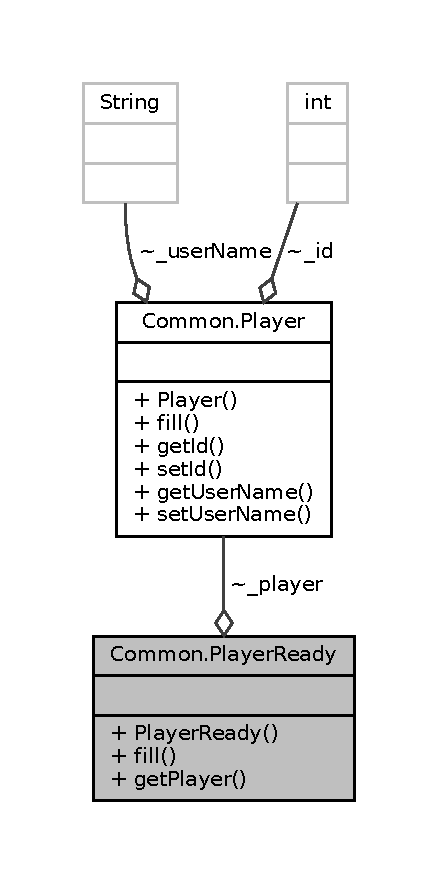
\includegraphics[width=210pt]{classCommon_1_1PlayerReady__coll__graph}
\end{center}
\end{figure}
\subsection*{Public Member Functions}
\begin{DoxyCompactItemize}
\item 
\mbox{\hyperlink{classCommon_1_1PlayerReady_a1ff6236d6f61b61f89955f2f2d618118}{Player\+Ready}} ()
\item 
\mbox{\hyperlink{classCommon_1_1PlayerReady}{Player\+Ready}} \mbox{\hyperlink{classCommon_1_1PlayerReady_af47dc94fb6f6eef26e062fb211ec173a}{fill}} (\mbox{\hyperlink{classCommon_1_1Player}{Player}} player)
\item 
\mbox{\hyperlink{classCommon_1_1Player}{Player}} \mbox{\hyperlink{classCommon_1_1PlayerReady_aa64f37b079e34f6e9a74416f68d334a5}{get\+Player}} ()
\end{DoxyCompactItemize}


\subsection{Constructor \& Destructor Documentation}
\mbox{\Hypertarget{classCommon_1_1PlayerReady_a1ff6236d6f61b61f89955f2f2d618118}\label{classCommon_1_1PlayerReady_a1ff6236d6f61b61f89955f2f2d618118}} 
\index{Common\+::\+Player\+Ready@{Common\+::\+Player\+Ready}!Player\+Ready@{Player\+Ready}}
\index{Player\+Ready@{Player\+Ready}!Common\+::\+Player\+Ready@{Common\+::\+Player\+Ready}}
\subsubsection{\texorpdfstring{Player\+Ready()}{PlayerReady()}}
{\footnotesize\ttfamily Common.\+Player\+Ready.\+Player\+Ready (\begin{DoxyParamCaption}{ }\end{DoxyParamCaption})\hspace{0.3cm}{\ttfamily [inline]}}



\subsection{Member Function Documentation}
\mbox{\Hypertarget{classCommon_1_1PlayerReady_af47dc94fb6f6eef26e062fb211ec173a}\label{classCommon_1_1PlayerReady_af47dc94fb6f6eef26e062fb211ec173a}} 
\index{Common\+::\+Player\+Ready@{Common\+::\+Player\+Ready}!fill@{fill}}
\index{fill@{fill}!Common\+::\+Player\+Ready@{Common\+::\+Player\+Ready}}
\subsubsection{\texorpdfstring{fill()}{fill()}}
{\footnotesize\ttfamily \mbox{\hyperlink{classCommon_1_1PlayerReady}{Player\+Ready}} Common.\+Player\+Ready.\+fill (\begin{DoxyParamCaption}\item[{\mbox{\hyperlink{classCommon_1_1Player}{Player}}}]{player }\end{DoxyParamCaption})\hspace{0.3cm}{\ttfamily [inline]}}

\mbox{\Hypertarget{classCommon_1_1PlayerReady_aa64f37b079e34f6e9a74416f68d334a5}\label{classCommon_1_1PlayerReady_aa64f37b079e34f6e9a74416f68d334a5}} 
\index{Common\+::\+Player\+Ready@{Common\+::\+Player\+Ready}!get\+Player@{get\+Player}}
\index{get\+Player@{get\+Player}!Common\+::\+Player\+Ready@{Common\+::\+Player\+Ready}}
\subsubsection{\texorpdfstring{get\+Player()}{getPlayer()}}
{\footnotesize\ttfamily \mbox{\hyperlink{classCommon_1_1Player}{Player}} Common.\+Player\+Ready.\+get\+Player (\begin{DoxyParamCaption}{ }\end{DoxyParamCaption})\hspace{0.3cm}{\ttfamily [inline]}}



The documentation for this class was generated from the following file\+:\begin{DoxyCompactItemize}
\item 
/home/tetard/\+Idea\+Projects/j\+Coinche/\+Java\+\_\+jcoinche\+\_\+2017/src/main/java/\+Common/\mbox{\hyperlink{PlayerReady_8java}{Player\+Ready.\+java}}\end{DoxyCompactItemize}

\hypertarget{enumClient_1_1Model_1_1ReadyState}{}\section{Client.\+Model.\+Ready\+State Enum Reference}
\label{enumClient_1_1Model_1_1ReadyState}\index{Client.\+Model.\+Ready\+State@{Client.\+Model.\+Ready\+State}}


Collaboration diagram for Client.\+Model.\+Ready\+State\+:
\nopagebreak
\begin{figure}[H]
\begin{center}
\leavevmode
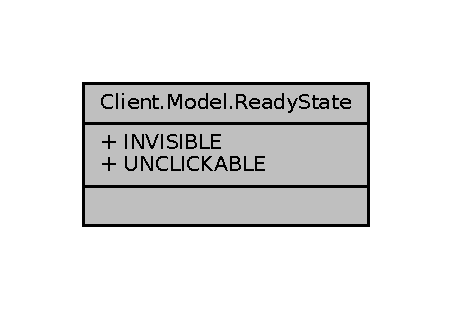
\includegraphics[width=217pt]{enumClient_1_1Model_1_1ReadyState__coll__graph}
\end{center}
\end{figure}
\subsection*{Public Attributes}
\begin{DoxyCompactItemize}
\item 
\mbox{\hyperlink{enumClient_1_1Model_1_1ReadyState_a1af85003e6591619effc0216684d9235}{I\+N\+V\+I\+S\+I\+B\+LE}}
\item 
\mbox{\hyperlink{enumClient_1_1Model_1_1ReadyState_acd3251fb20416d6aa8ea238102f3d9f2}{U\+N\+C\+L\+I\+C\+K\+A\+B\+LE}}
\end{DoxyCompactItemize}


\subsection{Member Data Documentation}
\mbox{\Hypertarget{enumClient_1_1Model_1_1ReadyState_a1af85003e6591619effc0216684d9235}\label{enumClient_1_1Model_1_1ReadyState_a1af85003e6591619effc0216684d9235}} 
\index{Client\+::\+Model\+::\+Ready\+State@{Client\+::\+Model\+::\+Ready\+State}!I\+N\+V\+I\+S\+I\+B\+LE@{I\+N\+V\+I\+S\+I\+B\+LE}}
\index{I\+N\+V\+I\+S\+I\+B\+LE@{I\+N\+V\+I\+S\+I\+B\+LE}!Client\+::\+Model\+::\+Ready\+State@{Client\+::\+Model\+::\+Ready\+State}}
\subsubsection{\texorpdfstring{I\+N\+V\+I\+S\+I\+B\+LE}{INVISIBLE}}
{\footnotesize\ttfamily Client.\+Model.\+Ready\+State.\+I\+N\+V\+I\+S\+I\+B\+LE}

\mbox{\Hypertarget{enumClient_1_1Model_1_1ReadyState_acd3251fb20416d6aa8ea238102f3d9f2}\label{enumClient_1_1Model_1_1ReadyState_acd3251fb20416d6aa8ea238102f3d9f2}} 
\index{Client\+::\+Model\+::\+Ready\+State@{Client\+::\+Model\+::\+Ready\+State}!U\+N\+C\+L\+I\+C\+K\+A\+B\+LE@{U\+N\+C\+L\+I\+C\+K\+A\+B\+LE}}
\index{U\+N\+C\+L\+I\+C\+K\+A\+B\+LE@{U\+N\+C\+L\+I\+C\+K\+A\+B\+LE}!Client\+::\+Model\+::\+Ready\+State@{Client\+::\+Model\+::\+Ready\+State}}
\subsubsection{\texorpdfstring{U\+N\+C\+L\+I\+C\+K\+A\+B\+LE}{UNCLICKABLE}}
{\footnotesize\ttfamily Client.\+Model.\+Ready\+State.\+U\+N\+C\+L\+I\+C\+K\+A\+B\+LE}



The documentation for this enum was generated from the following file\+:\begin{DoxyCompactItemize}
\item 
/home/tetard/\+Idea\+Projects/j\+Coinche/\+Java\+\_\+jcoinche\+\_\+2017/src/main/java/\+Client/\+Model/\mbox{\hyperlink{ReadyState_8java}{Ready\+State.\+java}}\end{DoxyCompactItemize}

\hypertarget{classServer_1_1ServerConnexion_1_1RequestHandler}{}\section{Server.\+Server\+Connexion.\+Request\+Handler Class Reference}
\label{classServer_1_1ServerConnexion_1_1RequestHandler}\index{Server.\+Server\+Connexion.\+Request\+Handler@{Server.\+Server\+Connexion.\+Request\+Handler}}


Collaboration diagram for Server.\+Server\+Connexion.\+Request\+Handler\+:
\nopagebreak
\begin{figure}[H]
\begin{center}
\leavevmode
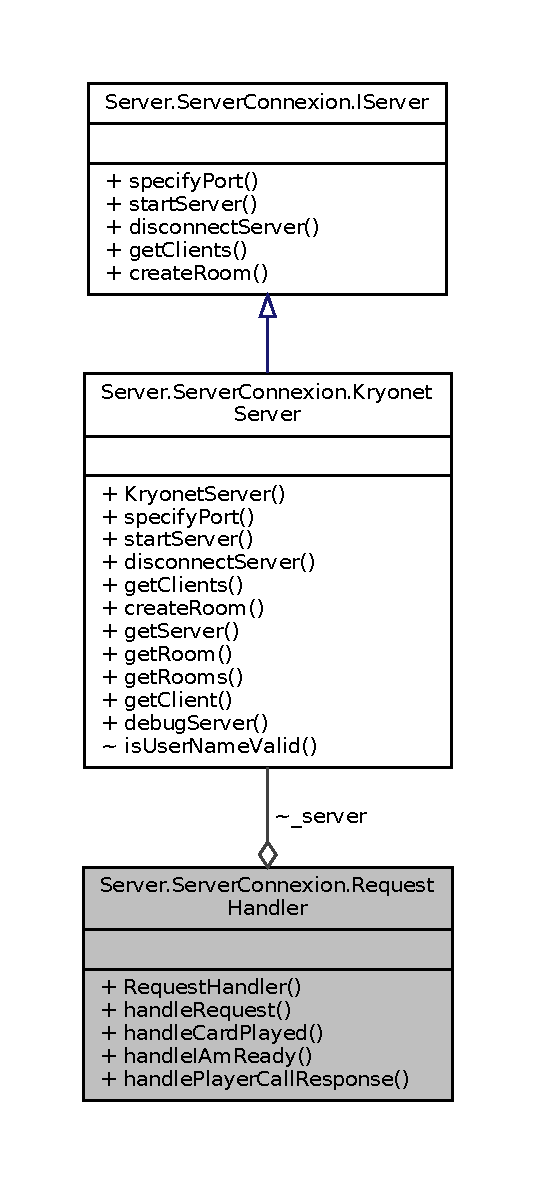
\includegraphics[height=550pt]{classServer_1_1ServerConnexion_1_1RequestHandler__coll__graph}
\end{center}
\end{figure}
\subsection*{Public Member Functions}
\begin{DoxyCompactItemize}
\item 
\mbox{\hyperlink{classServer_1_1ServerConnexion_1_1RequestHandler_a4cedcc90cb128b9781735e8149fa4801}{Request\+Handler}} (\mbox{\hyperlink{classServer_1_1ServerConnexion_1_1KryonetServer}{Kryonet\+Server}} server)
\item 
void \mbox{\hyperlink{classServer_1_1ServerConnexion_1_1RequestHandler_af8f168ba8f0f372af423c44d87dec13f}{handle\+Request}} (\mbox{\hyperlink{classServer_1_1ServerConnexion_1_1ClientInfos}{Client\+Infos}} client, Object o)
\item 
void \mbox{\hyperlink{classServer_1_1ServerConnexion_1_1RequestHandler_a0a48f220efcfc97fca14564ce8daa43e}{handle\+Card\+Played}} (\mbox{\hyperlink{classServer_1_1ServerConnexion_1_1ClientInfos}{Client\+Infos}} client, \mbox{\hyperlink{classCommon_1_1CardPlayed}{Card\+Played}} o)
\item 
void \mbox{\hyperlink{classServer_1_1ServerConnexion_1_1RequestHandler_a490c790aa95eea47bd51f380e030729d}{handle\+I\+Am\+Ready}} (\mbox{\hyperlink{classServer_1_1ServerConnexion_1_1ClientInfos}{Client\+Infos}} client, \mbox{\hyperlink{classCommon_1_1IAmReady}{I\+Am\+Ready}} o)
\item 
void \mbox{\hyperlink{classServer_1_1ServerConnexion_1_1RequestHandler_a87669742b2b85431cad3084999fa31e5}{handle\+Player\+Call\+Response}} (\mbox{\hyperlink{classServer_1_1ServerConnexion_1_1ClientInfos}{Client\+Infos}} client, \mbox{\hyperlink{classCommon_1_1PlayerCallResponse}{Player\+Call\+Response}} o)
\end{DoxyCompactItemize}


\subsection{Constructor \& Destructor Documentation}
\mbox{\Hypertarget{classServer_1_1ServerConnexion_1_1RequestHandler_a4cedcc90cb128b9781735e8149fa4801}\label{classServer_1_1ServerConnexion_1_1RequestHandler_a4cedcc90cb128b9781735e8149fa4801}} 
\index{Server\+::\+Server\+Connexion\+::\+Request\+Handler@{Server\+::\+Server\+Connexion\+::\+Request\+Handler}!Request\+Handler@{Request\+Handler}}
\index{Request\+Handler@{Request\+Handler}!Server\+::\+Server\+Connexion\+::\+Request\+Handler@{Server\+::\+Server\+Connexion\+::\+Request\+Handler}}
\subsubsection{\texorpdfstring{Request\+Handler()}{RequestHandler()}}
{\footnotesize\ttfamily Server.\+Server\+Connexion.\+Request\+Handler.\+Request\+Handler (\begin{DoxyParamCaption}\item[{\mbox{\hyperlink{classServer_1_1ServerConnexion_1_1KryonetServer}{Kryonet\+Server}}}]{server }\end{DoxyParamCaption})\hspace{0.3cm}{\ttfamily [inline]}}



\subsection{Member Function Documentation}
\mbox{\Hypertarget{classServer_1_1ServerConnexion_1_1RequestHandler_a0a48f220efcfc97fca14564ce8daa43e}\label{classServer_1_1ServerConnexion_1_1RequestHandler_a0a48f220efcfc97fca14564ce8daa43e}} 
\index{Server\+::\+Server\+Connexion\+::\+Request\+Handler@{Server\+::\+Server\+Connexion\+::\+Request\+Handler}!handle\+Card\+Played@{handle\+Card\+Played}}
\index{handle\+Card\+Played@{handle\+Card\+Played}!Server\+::\+Server\+Connexion\+::\+Request\+Handler@{Server\+::\+Server\+Connexion\+::\+Request\+Handler}}
\subsubsection{\texorpdfstring{handle\+Card\+Played()}{handleCardPlayed()}}
{\footnotesize\ttfamily void Server.\+Server\+Connexion.\+Request\+Handler.\+handle\+Card\+Played (\begin{DoxyParamCaption}\item[{\mbox{\hyperlink{classServer_1_1ServerConnexion_1_1ClientInfos}{Client\+Infos}}}]{client,  }\item[{\mbox{\hyperlink{classCommon_1_1CardPlayed}{Card\+Played}}}]{o }\end{DoxyParamCaption})\hspace{0.3cm}{\ttfamily [inline]}}

\mbox{\Hypertarget{classServer_1_1ServerConnexion_1_1RequestHandler_a490c790aa95eea47bd51f380e030729d}\label{classServer_1_1ServerConnexion_1_1RequestHandler_a490c790aa95eea47bd51f380e030729d}} 
\index{Server\+::\+Server\+Connexion\+::\+Request\+Handler@{Server\+::\+Server\+Connexion\+::\+Request\+Handler}!handle\+I\+Am\+Ready@{handle\+I\+Am\+Ready}}
\index{handle\+I\+Am\+Ready@{handle\+I\+Am\+Ready}!Server\+::\+Server\+Connexion\+::\+Request\+Handler@{Server\+::\+Server\+Connexion\+::\+Request\+Handler}}
\subsubsection{\texorpdfstring{handle\+I\+Am\+Ready()}{handleIAmReady()}}
{\footnotesize\ttfamily void Server.\+Server\+Connexion.\+Request\+Handler.\+handle\+I\+Am\+Ready (\begin{DoxyParamCaption}\item[{\mbox{\hyperlink{classServer_1_1ServerConnexion_1_1ClientInfos}{Client\+Infos}}}]{client,  }\item[{\mbox{\hyperlink{classCommon_1_1IAmReady}{I\+Am\+Ready}}}]{o }\end{DoxyParamCaption})\hspace{0.3cm}{\ttfamily [inline]}}

\mbox{\Hypertarget{classServer_1_1ServerConnexion_1_1RequestHandler_a87669742b2b85431cad3084999fa31e5}\label{classServer_1_1ServerConnexion_1_1RequestHandler_a87669742b2b85431cad3084999fa31e5}} 
\index{Server\+::\+Server\+Connexion\+::\+Request\+Handler@{Server\+::\+Server\+Connexion\+::\+Request\+Handler}!handle\+Player\+Call\+Response@{handle\+Player\+Call\+Response}}
\index{handle\+Player\+Call\+Response@{handle\+Player\+Call\+Response}!Server\+::\+Server\+Connexion\+::\+Request\+Handler@{Server\+::\+Server\+Connexion\+::\+Request\+Handler}}
\subsubsection{\texorpdfstring{handle\+Player\+Call\+Response()}{handlePlayerCallResponse()}}
{\footnotesize\ttfamily void Server.\+Server\+Connexion.\+Request\+Handler.\+handle\+Player\+Call\+Response (\begin{DoxyParamCaption}\item[{\mbox{\hyperlink{classServer_1_1ServerConnexion_1_1ClientInfos}{Client\+Infos}}}]{client,  }\item[{\mbox{\hyperlink{classCommon_1_1PlayerCallResponse}{Player\+Call\+Response}}}]{o }\end{DoxyParamCaption})\hspace{0.3cm}{\ttfamily [inline]}}

\mbox{\Hypertarget{classServer_1_1ServerConnexion_1_1RequestHandler_af8f168ba8f0f372af423c44d87dec13f}\label{classServer_1_1ServerConnexion_1_1RequestHandler_af8f168ba8f0f372af423c44d87dec13f}} 
\index{Server\+::\+Server\+Connexion\+::\+Request\+Handler@{Server\+::\+Server\+Connexion\+::\+Request\+Handler}!handle\+Request@{handle\+Request}}
\index{handle\+Request@{handle\+Request}!Server\+::\+Server\+Connexion\+::\+Request\+Handler@{Server\+::\+Server\+Connexion\+::\+Request\+Handler}}
\subsubsection{\texorpdfstring{handle\+Request()}{handleRequest()}}
{\footnotesize\ttfamily void Server.\+Server\+Connexion.\+Request\+Handler.\+handle\+Request (\begin{DoxyParamCaption}\item[{\mbox{\hyperlink{classServer_1_1ServerConnexion_1_1ClientInfos}{Client\+Infos}}}]{client,  }\item[{Object}]{o }\end{DoxyParamCaption})\hspace{0.3cm}{\ttfamily [inline]}}



The documentation for this class was generated from the following file\+:\begin{DoxyCompactItemize}
\item 
/home/tetard/\+Idea\+Projects/j\+Coinche/\+Java\+\_\+jcoinche\+\_\+2017/src/main/java/\+Server/\+Server\+Connexion/\mbox{\hyperlink{RequestHandler_8java}{Request\+Handler.\+java}}\end{DoxyCompactItemize}

\hypertarget{classServer_1_1ServerConnexion_1_1Room}{}\section{Server.\+Server\+Connexion.\+Room Class Reference}
\label{classServer_1_1ServerConnexion_1_1Room}\index{Server.\+Server\+Connexion.\+Room@{Server.\+Server\+Connexion.\+Room}}


Collaboration diagram for Server.\+Server\+Connexion.\+Room\+:
\nopagebreak
\begin{figure}[H]
\begin{center}
\leavevmode
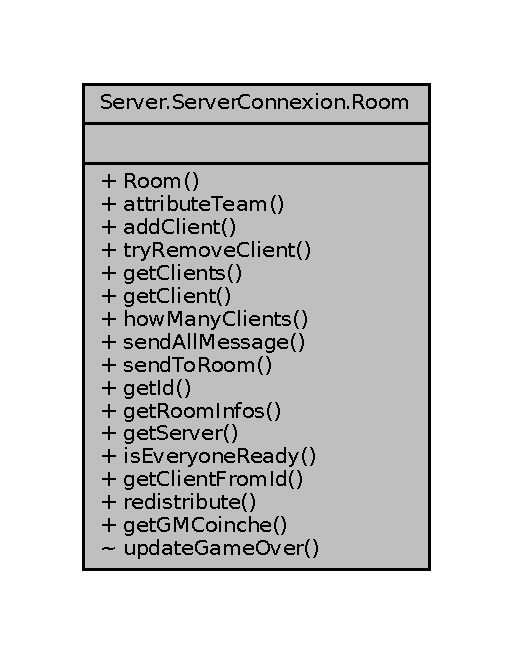
\includegraphics[width=246pt]{classServer_1_1ServerConnexion_1_1Room__coll__graph}
\end{center}
\end{figure}
\subsection*{Public Member Functions}
\begin{DoxyCompactItemize}
\item 
\mbox{\hyperlink{classServer_1_1ServerConnexion_1_1Room_a191c2d5940dc3c6cb1fece18e879a64d}{Room}} (int id, \mbox{\hyperlink{classServer_1_1ServerConnexion_1_1ClientInfos}{Client\+Infos}} client, Server server, Concurrent\+Hash\+Map$<$ Integer, \mbox{\hyperlink{classServer_1_1ServerConnexion_1_1ClientInfos}{Client\+Infos}} $>$ clients)
\item 
void \mbox{\hyperlink{classServer_1_1ServerConnexion_1_1Room_a1c5bc1300ad6c1be3019e20fc44bce79}{attribute\+Team}} ()
\item 
void \mbox{\hyperlink{classServer_1_1ServerConnexion_1_1Room_afc78e8884ccced8e6ccddcdf9c3b0d81}{add\+Client}} (\mbox{\hyperlink{classServer_1_1ServerConnexion_1_1ClientInfos}{Client\+Infos}} client)
\item 
boolean \mbox{\hyperlink{classServer_1_1ServerConnexion_1_1Room_a5b478e86f07cb7f40db27f8db26fb955}{try\+Remove\+Client}} (Integer id, Concurrent\+Hash\+Map$<$ Integer, \mbox{\hyperlink{classServer_1_1ServerConnexion_1_1Room}{Room}} $>$ room\+List)
\item 
Array\+List$<$ \mbox{\hyperlink{classServer_1_1ServerConnexion_1_1ClientInfos}{Client\+Infos}} $>$ \mbox{\hyperlink{classServer_1_1ServerConnexion_1_1Room_aa8d4955026b246208bfda5e6a1199e86}{get\+Clients}} ()
\item 
\mbox{\hyperlink{classServer_1_1ServerConnexion_1_1ClientInfos}{Client\+Infos}} \mbox{\hyperlink{classServer_1_1ServerConnexion_1_1Room_a22d44a6dcc0a72fb36c1be8d355c1f53}{get\+Client}} (int idx)
\item 
int \mbox{\hyperlink{classServer_1_1ServerConnexion_1_1Room_a952b0f724c1f5e04a78a70dfed594c20}{how\+Many\+Clients}} ()
\item 
void \mbox{\hyperlink{classServer_1_1ServerConnexion_1_1Room_a53c24cabf3f30a8aff5e4a563d5f08d7}{send\+All\+Message}} (Object o)
\item 
void \mbox{\hyperlink{classServer_1_1ServerConnexion_1_1Room_a7cd935fd7d302c107bb42d8c7faf5d75}{send\+To\+Room}} (Object o)
\item 
int \mbox{\hyperlink{classServer_1_1ServerConnexion_1_1Room_a14346f0160466c67d28dbf45926225b2}{get\+Id}} ()
\item 
\mbox{\hyperlink{classCommon_1_1RoomInfo}{Room\+Info}} \mbox{\hyperlink{classServer_1_1ServerConnexion_1_1Room_a770cf7370fbcf6cef279f4ea260159fe}{get\+Room\+Infos}} ()
\item 
Server \mbox{\hyperlink{classServer_1_1ServerConnexion_1_1Room_a82aa25bc3f5406ce06589c92f12f59e1}{get\+Server}} ()
\item 
boolean \mbox{\hyperlink{classServer_1_1ServerConnexion_1_1Room_a2e67e0da5adef24542d2082828e75a88}{is\+Everyone\+Ready}} ()
\item 
\mbox{\hyperlink{classServer_1_1ServerConnexion_1_1ClientInfos}{Client\+Infos}} \mbox{\hyperlink{classServer_1_1ServerConnexion_1_1Room_a60fc7bece76f7b765c2d32501af4d960}{get\+Client\+From\+Id}} (int id)
\item 
void \mbox{\hyperlink{classServer_1_1ServerConnexion_1_1Room_a6a2dd1ea8ed605869b42d4b2a183acc4}{redistribute}} ()
\item 
\mbox{\hyperlink{classServer_1_1Game_1_1GameMasterCoinche}{Game\+Master\+Coinche}} \mbox{\hyperlink{classServer_1_1ServerConnexion_1_1Room_aa7f336575bfad4b96f80c164f41d1517}{get\+G\+M\+Coinche}} ()
\end{DoxyCompactItemize}


\subsection{Constructor \& Destructor Documentation}
\mbox{\Hypertarget{classServer_1_1ServerConnexion_1_1Room_a191c2d5940dc3c6cb1fece18e879a64d}\label{classServer_1_1ServerConnexion_1_1Room_a191c2d5940dc3c6cb1fece18e879a64d}} 
\index{Server\+::\+Server\+Connexion\+::\+Room@{Server\+::\+Server\+Connexion\+::\+Room}!Room@{Room}}
\index{Room@{Room}!Server\+::\+Server\+Connexion\+::\+Room@{Server\+::\+Server\+Connexion\+::\+Room}}
\subsubsection{\texorpdfstring{Room()}{Room()}}
{\footnotesize\ttfamily Server.\+Server\+Connexion.\+Room.\+Room (\begin{DoxyParamCaption}\item[{int}]{id,  }\item[{\mbox{\hyperlink{classServer_1_1ServerConnexion_1_1ClientInfos}{Client\+Infos}}}]{client,  }\item[{Server}]{server,  }\item[{Concurrent\+Hash\+Map$<$ Integer, \mbox{\hyperlink{classServer_1_1ServerConnexion_1_1ClientInfos}{Client\+Infos}} $>$}]{clients }\end{DoxyParamCaption})\hspace{0.3cm}{\ttfamily [inline]}}



\subsection{Member Function Documentation}
\mbox{\Hypertarget{classServer_1_1ServerConnexion_1_1Room_afc78e8884ccced8e6ccddcdf9c3b0d81}\label{classServer_1_1ServerConnexion_1_1Room_afc78e8884ccced8e6ccddcdf9c3b0d81}} 
\index{Server\+::\+Server\+Connexion\+::\+Room@{Server\+::\+Server\+Connexion\+::\+Room}!add\+Client@{add\+Client}}
\index{add\+Client@{add\+Client}!Server\+::\+Server\+Connexion\+::\+Room@{Server\+::\+Server\+Connexion\+::\+Room}}
\subsubsection{\texorpdfstring{add\+Client()}{addClient()}}
{\footnotesize\ttfamily void Server.\+Server\+Connexion.\+Room.\+add\+Client (\begin{DoxyParamCaption}\item[{\mbox{\hyperlink{classServer_1_1ServerConnexion_1_1ClientInfos}{Client\+Infos}}}]{client }\end{DoxyParamCaption})\hspace{0.3cm}{\ttfamily [inline]}}

\mbox{\Hypertarget{classServer_1_1ServerConnexion_1_1Room_a1c5bc1300ad6c1be3019e20fc44bce79}\label{classServer_1_1ServerConnexion_1_1Room_a1c5bc1300ad6c1be3019e20fc44bce79}} 
\index{Server\+::\+Server\+Connexion\+::\+Room@{Server\+::\+Server\+Connexion\+::\+Room}!attribute\+Team@{attribute\+Team}}
\index{attribute\+Team@{attribute\+Team}!Server\+::\+Server\+Connexion\+::\+Room@{Server\+::\+Server\+Connexion\+::\+Room}}
\subsubsection{\texorpdfstring{attribute\+Team()}{attributeTeam()}}
{\footnotesize\ttfamily void Server.\+Server\+Connexion.\+Room.\+attribute\+Team (\begin{DoxyParamCaption}{ }\end{DoxyParamCaption})\hspace{0.3cm}{\ttfamily [inline]}}

\mbox{\Hypertarget{classServer_1_1ServerConnexion_1_1Room_a22d44a6dcc0a72fb36c1be8d355c1f53}\label{classServer_1_1ServerConnexion_1_1Room_a22d44a6dcc0a72fb36c1be8d355c1f53}} 
\index{Server\+::\+Server\+Connexion\+::\+Room@{Server\+::\+Server\+Connexion\+::\+Room}!get\+Client@{get\+Client}}
\index{get\+Client@{get\+Client}!Server\+::\+Server\+Connexion\+::\+Room@{Server\+::\+Server\+Connexion\+::\+Room}}
\subsubsection{\texorpdfstring{get\+Client()}{getClient()}}
{\footnotesize\ttfamily \mbox{\hyperlink{classServer_1_1ServerConnexion_1_1ClientInfos}{Client\+Infos}} Server.\+Server\+Connexion.\+Room.\+get\+Client (\begin{DoxyParamCaption}\item[{int}]{idx }\end{DoxyParamCaption})\hspace{0.3cm}{\ttfamily [inline]}}

\mbox{\Hypertarget{classServer_1_1ServerConnexion_1_1Room_a60fc7bece76f7b765c2d32501af4d960}\label{classServer_1_1ServerConnexion_1_1Room_a60fc7bece76f7b765c2d32501af4d960}} 
\index{Server\+::\+Server\+Connexion\+::\+Room@{Server\+::\+Server\+Connexion\+::\+Room}!get\+Client\+From\+Id@{get\+Client\+From\+Id}}
\index{get\+Client\+From\+Id@{get\+Client\+From\+Id}!Server\+::\+Server\+Connexion\+::\+Room@{Server\+::\+Server\+Connexion\+::\+Room}}
\subsubsection{\texorpdfstring{get\+Client\+From\+Id()}{getClientFromId()}}
{\footnotesize\ttfamily \mbox{\hyperlink{classServer_1_1ServerConnexion_1_1ClientInfos}{Client\+Infos}} Server.\+Server\+Connexion.\+Room.\+get\+Client\+From\+Id (\begin{DoxyParamCaption}\item[{int}]{id }\end{DoxyParamCaption})\hspace{0.3cm}{\ttfamily [inline]}}

\mbox{\Hypertarget{classServer_1_1ServerConnexion_1_1Room_aa8d4955026b246208bfda5e6a1199e86}\label{classServer_1_1ServerConnexion_1_1Room_aa8d4955026b246208bfda5e6a1199e86}} 
\index{Server\+::\+Server\+Connexion\+::\+Room@{Server\+::\+Server\+Connexion\+::\+Room}!get\+Clients@{get\+Clients}}
\index{get\+Clients@{get\+Clients}!Server\+::\+Server\+Connexion\+::\+Room@{Server\+::\+Server\+Connexion\+::\+Room}}
\subsubsection{\texorpdfstring{get\+Clients()}{getClients()}}
{\footnotesize\ttfamily Array\+List$<$\mbox{\hyperlink{classServer_1_1ServerConnexion_1_1ClientInfos}{Client\+Infos}}$>$ Server.\+Server\+Connexion.\+Room.\+get\+Clients (\begin{DoxyParamCaption}{ }\end{DoxyParamCaption})\hspace{0.3cm}{\ttfamily [inline]}}

\mbox{\Hypertarget{classServer_1_1ServerConnexion_1_1Room_aa7f336575bfad4b96f80c164f41d1517}\label{classServer_1_1ServerConnexion_1_1Room_aa7f336575bfad4b96f80c164f41d1517}} 
\index{Server\+::\+Server\+Connexion\+::\+Room@{Server\+::\+Server\+Connexion\+::\+Room}!get\+G\+M\+Coinche@{get\+G\+M\+Coinche}}
\index{get\+G\+M\+Coinche@{get\+G\+M\+Coinche}!Server\+::\+Server\+Connexion\+::\+Room@{Server\+::\+Server\+Connexion\+::\+Room}}
\subsubsection{\texorpdfstring{get\+G\+M\+Coinche()}{getGMCoinche()}}
{\footnotesize\ttfamily \mbox{\hyperlink{classServer_1_1Game_1_1GameMasterCoinche}{Game\+Master\+Coinche}} Server.\+Server\+Connexion.\+Room.\+get\+G\+M\+Coinche (\begin{DoxyParamCaption}{ }\end{DoxyParamCaption})\hspace{0.3cm}{\ttfamily [inline]}}

\mbox{\Hypertarget{classServer_1_1ServerConnexion_1_1Room_a14346f0160466c67d28dbf45926225b2}\label{classServer_1_1ServerConnexion_1_1Room_a14346f0160466c67d28dbf45926225b2}} 
\index{Server\+::\+Server\+Connexion\+::\+Room@{Server\+::\+Server\+Connexion\+::\+Room}!get\+Id@{get\+Id}}
\index{get\+Id@{get\+Id}!Server\+::\+Server\+Connexion\+::\+Room@{Server\+::\+Server\+Connexion\+::\+Room}}
\subsubsection{\texorpdfstring{get\+Id()}{getId()}}
{\footnotesize\ttfamily int Server.\+Server\+Connexion.\+Room.\+get\+Id (\begin{DoxyParamCaption}{ }\end{DoxyParamCaption})\hspace{0.3cm}{\ttfamily [inline]}}

\mbox{\Hypertarget{classServer_1_1ServerConnexion_1_1Room_a770cf7370fbcf6cef279f4ea260159fe}\label{classServer_1_1ServerConnexion_1_1Room_a770cf7370fbcf6cef279f4ea260159fe}} 
\index{Server\+::\+Server\+Connexion\+::\+Room@{Server\+::\+Server\+Connexion\+::\+Room}!get\+Room\+Infos@{get\+Room\+Infos}}
\index{get\+Room\+Infos@{get\+Room\+Infos}!Server\+::\+Server\+Connexion\+::\+Room@{Server\+::\+Server\+Connexion\+::\+Room}}
\subsubsection{\texorpdfstring{get\+Room\+Infos()}{getRoomInfos()}}
{\footnotesize\ttfamily \mbox{\hyperlink{classCommon_1_1RoomInfo}{Room\+Info}} Server.\+Server\+Connexion.\+Room.\+get\+Room\+Infos (\begin{DoxyParamCaption}{ }\end{DoxyParamCaption})\hspace{0.3cm}{\ttfamily [inline]}}

\mbox{\Hypertarget{classServer_1_1ServerConnexion_1_1Room_a82aa25bc3f5406ce06589c92f12f59e1}\label{classServer_1_1ServerConnexion_1_1Room_a82aa25bc3f5406ce06589c92f12f59e1}} 
\index{Server\+::\+Server\+Connexion\+::\+Room@{Server\+::\+Server\+Connexion\+::\+Room}!get\+Server@{get\+Server}}
\index{get\+Server@{get\+Server}!Server\+::\+Server\+Connexion\+::\+Room@{Server\+::\+Server\+Connexion\+::\+Room}}
\subsubsection{\texorpdfstring{get\+Server()}{getServer()}}
{\footnotesize\ttfamily Server Server.\+Server\+Connexion.\+Room.\+get\+Server (\begin{DoxyParamCaption}{ }\end{DoxyParamCaption})\hspace{0.3cm}{\ttfamily [inline]}}

\mbox{\Hypertarget{classServer_1_1ServerConnexion_1_1Room_a952b0f724c1f5e04a78a70dfed594c20}\label{classServer_1_1ServerConnexion_1_1Room_a952b0f724c1f5e04a78a70dfed594c20}} 
\index{Server\+::\+Server\+Connexion\+::\+Room@{Server\+::\+Server\+Connexion\+::\+Room}!how\+Many\+Clients@{how\+Many\+Clients}}
\index{how\+Many\+Clients@{how\+Many\+Clients}!Server\+::\+Server\+Connexion\+::\+Room@{Server\+::\+Server\+Connexion\+::\+Room}}
\subsubsection{\texorpdfstring{how\+Many\+Clients()}{howManyClients()}}
{\footnotesize\ttfamily int Server.\+Server\+Connexion.\+Room.\+how\+Many\+Clients (\begin{DoxyParamCaption}{ }\end{DoxyParamCaption})\hspace{0.3cm}{\ttfamily [inline]}}

\mbox{\Hypertarget{classServer_1_1ServerConnexion_1_1Room_a2e67e0da5adef24542d2082828e75a88}\label{classServer_1_1ServerConnexion_1_1Room_a2e67e0da5adef24542d2082828e75a88}} 
\index{Server\+::\+Server\+Connexion\+::\+Room@{Server\+::\+Server\+Connexion\+::\+Room}!is\+Everyone\+Ready@{is\+Everyone\+Ready}}
\index{is\+Everyone\+Ready@{is\+Everyone\+Ready}!Server\+::\+Server\+Connexion\+::\+Room@{Server\+::\+Server\+Connexion\+::\+Room}}
\subsubsection{\texorpdfstring{is\+Everyone\+Ready()}{isEveryoneReady()}}
{\footnotesize\ttfamily boolean Server.\+Server\+Connexion.\+Room.\+is\+Everyone\+Ready (\begin{DoxyParamCaption}{ }\end{DoxyParamCaption})\hspace{0.3cm}{\ttfamily [inline]}}

\mbox{\Hypertarget{classServer_1_1ServerConnexion_1_1Room_a6a2dd1ea8ed605869b42d4b2a183acc4}\label{classServer_1_1ServerConnexion_1_1Room_a6a2dd1ea8ed605869b42d4b2a183acc4}} 
\index{Server\+::\+Server\+Connexion\+::\+Room@{Server\+::\+Server\+Connexion\+::\+Room}!redistribute@{redistribute}}
\index{redistribute@{redistribute}!Server\+::\+Server\+Connexion\+::\+Room@{Server\+::\+Server\+Connexion\+::\+Room}}
\subsubsection{\texorpdfstring{redistribute()}{redistribute()}}
{\footnotesize\ttfamily void Server.\+Server\+Connexion.\+Room.\+redistribute (\begin{DoxyParamCaption}{ }\end{DoxyParamCaption})\hspace{0.3cm}{\ttfamily [inline]}}

\mbox{\Hypertarget{classServer_1_1ServerConnexion_1_1Room_a53c24cabf3f30a8aff5e4a563d5f08d7}\label{classServer_1_1ServerConnexion_1_1Room_a53c24cabf3f30a8aff5e4a563d5f08d7}} 
\index{Server\+::\+Server\+Connexion\+::\+Room@{Server\+::\+Server\+Connexion\+::\+Room}!send\+All\+Message@{send\+All\+Message}}
\index{send\+All\+Message@{send\+All\+Message}!Server\+::\+Server\+Connexion\+::\+Room@{Server\+::\+Server\+Connexion\+::\+Room}}
\subsubsection{\texorpdfstring{send\+All\+Message()}{sendAllMessage()}}
{\footnotesize\ttfamily void Server.\+Server\+Connexion.\+Room.\+send\+All\+Message (\begin{DoxyParamCaption}\item[{Object}]{o }\end{DoxyParamCaption})\hspace{0.3cm}{\ttfamily [inline]}}

\mbox{\Hypertarget{classServer_1_1ServerConnexion_1_1Room_a7cd935fd7d302c107bb42d8c7faf5d75}\label{classServer_1_1ServerConnexion_1_1Room_a7cd935fd7d302c107bb42d8c7faf5d75}} 
\index{Server\+::\+Server\+Connexion\+::\+Room@{Server\+::\+Server\+Connexion\+::\+Room}!send\+To\+Room@{send\+To\+Room}}
\index{send\+To\+Room@{send\+To\+Room}!Server\+::\+Server\+Connexion\+::\+Room@{Server\+::\+Server\+Connexion\+::\+Room}}
\subsubsection{\texorpdfstring{send\+To\+Room()}{sendToRoom()}}
{\footnotesize\ttfamily void Server.\+Server\+Connexion.\+Room.\+send\+To\+Room (\begin{DoxyParamCaption}\item[{Object}]{o }\end{DoxyParamCaption})\hspace{0.3cm}{\ttfamily [inline]}}

\mbox{\Hypertarget{classServer_1_1ServerConnexion_1_1Room_a5b478e86f07cb7f40db27f8db26fb955}\label{classServer_1_1ServerConnexion_1_1Room_a5b478e86f07cb7f40db27f8db26fb955}} 
\index{Server\+::\+Server\+Connexion\+::\+Room@{Server\+::\+Server\+Connexion\+::\+Room}!try\+Remove\+Client@{try\+Remove\+Client}}
\index{try\+Remove\+Client@{try\+Remove\+Client}!Server\+::\+Server\+Connexion\+::\+Room@{Server\+::\+Server\+Connexion\+::\+Room}}
\subsubsection{\texorpdfstring{try\+Remove\+Client()}{tryRemoveClient()}}
{\footnotesize\ttfamily boolean Server.\+Server\+Connexion.\+Room.\+try\+Remove\+Client (\begin{DoxyParamCaption}\item[{Integer}]{id,  }\item[{Concurrent\+Hash\+Map$<$ Integer, \mbox{\hyperlink{classServer_1_1ServerConnexion_1_1Room}{Room}} $>$}]{room\+List }\end{DoxyParamCaption})\hspace{0.3cm}{\ttfamily [inline]}}



The documentation for this class was generated from the following file\+:\begin{DoxyCompactItemize}
\item 
/home/tetard/\+Idea\+Projects/j\+Coinche/\+Java\+\_\+jcoinche\+\_\+2017/src/main/java/\+Server/\+Server\+Connexion/\mbox{\hyperlink{Room_8java}{Room.\+java}}\end{DoxyCompactItemize}

\hypertarget{classCommon_1_1RoomAccessAnswer}{}\section{Common.\+Room\+Access\+Answer Class Reference}
\label{classCommon_1_1RoomAccessAnswer}\index{Common.\+Room\+Access\+Answer@{Common.\+Room\+Access\+Answer}}


Collaboration diagram for Common.\+Room\+Access\+Answer\+:
\nopagebreak
\begin{figure}[H]
\begin{center}
\leavevmode
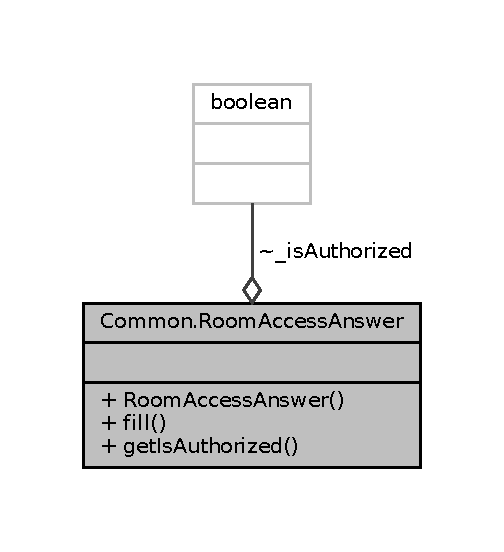
\includegraphics[width=242pt]{classCommon_1_1RoomAccessAnswer__coll__graph}
\end{center}
\end{figure}
\subsection*{Public Member Functions}
\begin{DoxyCompactItemize}
\item 
\mbox{\hyperlink{classCommon_1_1RoomAccessAnswer_a5127909913534ac7fe5ba604bd5bcf80}{Room\+Access\+Answer}} ()
\item 
\mbox{\hyperlink{classCommon_1_1RoomAccessAnswer}{Room\+Access\+Answer}} \mbox{\hyperlink{classCommon_1_1RoomAccessAnswer_abda9141bb331155f3cec2575a1b948c3}{fill}} (boolean is\+Authorized)
\item 
boolean \mbox{\hyperlink{classCommon_1_1RoomAccessAnswer_aca54d5af45356088e89548f3d7f2e137}{get\+Is\+Authorized}} ()
\end{DoxyCompactItemize}


\subsection{Constructor \& Destructor Documentation}
\mbox{\Hypertarget{classCommon_1_1RoomAccessAnswer_a5127909913534ac7fe5ba604bd5bcf80}\label{classCommon_1_1RoomAccessAnswer_a5127909913534ac7fe5ba604bd5bcf80}} 
\index{Common\+::\+Room\+Access\+Answer@{Common\+::\+Room\+Access\+Answer}!Room\+Access\+Answer@{Room\+Access\+Answer}}
\index{Room\+Access\+Answer@{Room\+Access\+Answer}!Common\+::\+Room\+Access\+Answer@{Common\+::\+Room\+Access\+Answer}}
\subsubsection{\texorpdfstring{Room\+Access\+Answer()}{RoomAccessAnswer()}}
{\footnotesize\ttfamily Common.\+Room\+Access\+Answer.\+Room\+Access\+Answer (\begin{DoxyParamCaption}{ }\end{DoxyParamCaption})\hspace{0.3cm}{\ttfamily [inline]}}



\subsection{Member Function Documentation}
\mbox{\Hypertarget{classCommon_1_1RoomAccessAnswer_abda9141bb331155f3cec2575a1b948c3}\label{classCommon_1_1RoomAccessAnswer_abda9141bb331155f3cec2575a1b948c3}} 
\index{Common\+::\+Room\+Access\+Answer@{Common\+::\+Room\+Access\+Answer}!fill@{fill}}
\index{fill@{fill}!Common\+::\+Room\+Access\+Answer@{Common\+::\+Room\+Access\+Answer}}
\subsubsection{\texorpdfstring{fill()}{fill()}}
{\footnotesize\ttfamily \mbox{\hyperlink{classCommon_1_1RoomAccessAnswer}{Room\+Access\+Answer}} Common.\+Room\+Access\+Answer.\+fill (\begin{DoxyParamCaption}\item[{boolean}]{is\+Authorized }\end{DoxyParamCaption})\hspace{0.3cm}{\ttfamily [inline]}}

\mbox{\Hypertarget{classCommon_1_1RoomAccessAnswer_aca54d5af45356088e89548f3d7f2e137}\label{classCommon_1_1RoomAccessAnswer_aca54d5af45356088e89548f3d7f2e137}} 
\index{Common\+::\+Room\+Access\+Answer@{Common\+::\+Room\+Access\+Answer}!get\+Is\+Authorized@{get\+Is\+Authorized}}
\index{get\+Is\+Authorized@{get\+Is\+Authorized}!Common\+::\+Room\+Access\+Answer@{Common\+::\+Room\+Access\+Answer}}
\subsubsection{\texorpdfstring{get\+Is\+Authorized()}{getIsAuthorized()}}
{\footnotesize\ttfamily boolean Common.\+Room\+Access\+Answer.\+get\+Is\+Authorized (\begin{DoxyParamCaption}{ }\end{DoxyParamCaption})\hspace{0.3cm}{\ttfamily [inline]}}



The documentation for this class was generated from the following file\+:\begin{DoxyCompactItemize}
\item 
/home/tetard/\+Idea\+Projects/j\+Coinche/\+Java\+\_\+jcoinche\+\_\+2017/src/main/java/\+Common/\mbox{\hyperlink{RoomAccessAnswer_8java}{Room\+Access\+Answer.\+java}}\end{DoxyCompactItemize}

\hypertarget{classCommon_1_1RoomCreate}{}\section{Common.\+Room\+Create Class Reference}
\label{classCommon_1_1RoomCreate}\index{Common.\+Room\+Create@{Common.\+Room\+Create}}


Collaboration diagram for Common.\+Room\+Create\+:
\nopagebreak
\begin{figure}[H]
\begin{center}
\leavevmode
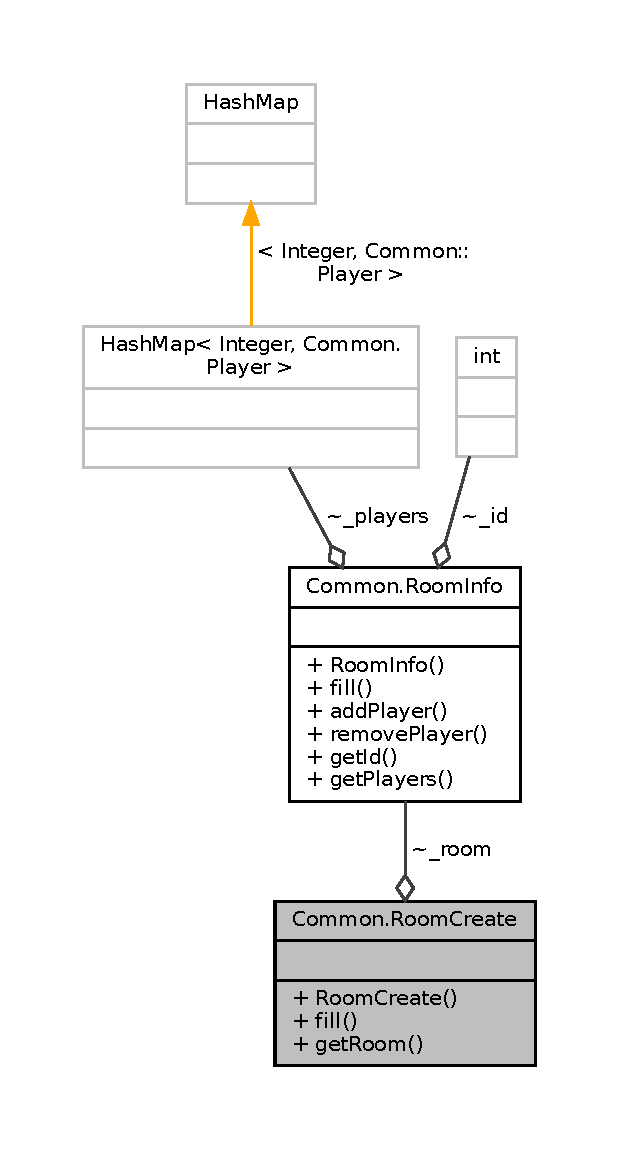
\includegraphics[height=550pt]{classCommon_1_1RoomCreate__coll__graph}
\end{center}
\end{figure}
\subsection*{Public Member Functions}
\begin{DoxyCompactItemize}
\item 
\mbox{\hyperlink{classCommon_1_1RoomCreate_ae06d6c403708490da9bc74396e9cc092}{Room\+Create}} ()
\item 
\mbox{\hyperlink{classCommon_1_1RoomCreate}{Room\+Create}} \mbox{\hyperlink{classCommon_1_1RoomCreate_ab779aabfd5c71281dcd36cf6dbfe4d11}{fill}} (\mbox{\hyperlink{classCommon_1_1RoomInfo}{Room\+Info}} room)
\item 
\mbox{\hyperlink{classCommon_1_1RoomInfo}{Room\+Info}} \mbox{\hyperlink{classCommon_1_1RoomCreate_a4bff6a47b84ef3350987e80977e0f017}{get\+Room}} ()
\end{DoxyCompactItemize}


\subsection{Constructor \& Destructor Documentation}
\mbox{\Hypertarget{classCommon_1_1RoomCreate_ae06d6c403708490da9bc74396e9cc092}\label{classCommon_1_1RoomCreate_ae06d6c403708490da9bc74396e9cc092}} 
\index{Common\+::\+Room\+Create@{Common\+::\+Room\+Create}!Room\+Create@{Room\+Create}}
\index{Room\+Create@{Room\+Create}!Common\+::\+Room\+Create@{Common\+::\+Room\+Create}}
\subsubsection{\texorpdfstring{Room\+Create()}{RoomCreate()}}
{\footnotesize\ttfamily Common.\+Room\+Create.\+Room\+Create (\begin{DoxyParamCaption}{ }\end{DoxyParamCaption})\hspace{0.3cm}{\ttfamily [inline]}}



\subsection{Member Function Documentation}
\mbox{\Hypertarget{classCommon_1_1RoomCreate_ab779aabfd5c71281dcd36cf6dbfe4d11}\label{classCommon_1_1RoomCreate_ab779aabfd5c71281dcd36cf6dbfe4d11}} 
\index{Common\+::\+Room\+Create@{Common\+::\+Room\+Create}!fill@{fill}}
\index{fill@{fill}!Common\+::\+Room\+Create@{Common\+::\+Room\+Create}}
\subsubsection{\texorpdfstring{fill()}{fill()}}
{\footnotesize\ttfamily \mbox{\hyperlink{classCommon_1_1RoomCreate}{Room\+Create}} Common.\+Room\+Create.\+fill (\begin{DoxyParamCaption}\item[{\mbox{\hyperlink{classCommon_1_1RoomInfo}{Room\+Info}}}]{room }\end{DoxyParamCaption})\hspace{0.3cm}{\ttfamily [inline]}}

\mbox{\Hypertarget{classCommon_1_1RoomCreate_a4bff6a47b84ef3350987e80977e0f017}\label{classCommon_1_1RoomCreate_a4bff6a47b84ef3350987e80977e0f017}} 
\index{Common\+::\+Room\+Create@{Common\+::\+Room\+Create}!get\+Room@{get\+Room}}
\index{get\+Room@{get\+Room}!Common\+::\+Room\+Create@{Common\+::\+Room\+Create}}
\subsubsection{\texorpdfstring{get\+Room()}{getRoom()}}
{\footnotesize\ttfamily \mbox{\hyperlink{classCommon_1_1RoomInfo}{Room\+Info}} Common.\+Room\+Create.\+get\+Room (\begin{DoxyParamCaption}{ }\end{DoxyParamCaption})\hspace{0.3cm}{\ttfamily [inline]}}



The documentation for this class was generated from the following file\+:\begin{DoxyCompactItemize}
\item 
/home/tetard/\+Idea\+Projects/j\+Coinche/\+Java\+\_\+jcoinche\+\_\+2017/src/main/java/\+Common/\mbox{\hyperlink{RoomCreate_8java}{Room\+Create.\+java}}\end{DoxyCompactItemize}

\hypertarget{classCommon_1_1RoomDeleted}{}\section{Common.\+Room\+Deleted Class Reference}
\label{classCommon_1_1RoomDeleted}\index{Common.\+Room\+Deleted@{Common.\+Room\+Deleted}}


Collaboration diagram for Common.\+Room\+Deleted\+:
\nopagebreak
\begin{figure}[H]
\begin{center}
\leavevmode
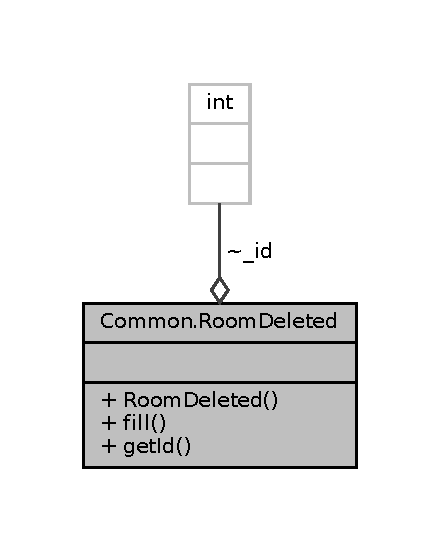
\includegraphics[width=211pt]{classCommon_1_1RoomDeleted__coll__graph}
\end{center}
\end{figure}
\subsection*{Public Member Functions}
\begin{DoxyCompactItemize}
\item 
\mbox{\hyperlink{classCommon_1_1RoomDeleted_ad4bb054370ba5dcb2296790d079d6884}{Room\+Deleted}} ()
\item 
\mbox{\hyperlink{classCommon_1_1RoomDeleted}{Room\+Deleted}} \mbox{\hyperlink{classCommon_1_1RoomDeleted_ab5c2f4c0eb47d43c35bdd9a44a448c8c}{fill}} (int id)
\item 
int \mbox{\hyperlink{classCommon_1_1RoomDeleted_a1c44d88d0acfd24f2a37a01205b27d94}{get\+Id}} ()
\end{DoxyCompactItemize}


\subsection{Constructor \& Destructor Documentation}
\mbox{\Hypertarget{classCommon_1_1RoomDeleted_ad4bb054370ba5dcb2296790d079d6884}\label{classCommon_1_1RoomDeleted_ad4bb054370ba5dcb2296790d079d6884}} 
\index{Common\+::\+Room\+Deleted@{Common\+::\+Room\+Deleted}!Room\+Deleted@{Room\+Deleted}}
\index{Room\+Deleted@{Room\+Deleted}!Common\+::\+Room\+Deleted@{Common\+::\+Room\+Deleted}}
\subsubsection{\texorpdfstring{Room\+Deleted()}{RoomDeleted()}}
{\footnotesize\ttfamily Common.\+Room\+Deleted.\+Room\+Deleted (\begin{DoxyParamCaption}{ }\end{DoxyParamCaption})\hspace{0.3cm}{\ttfamily [inline]}}



\subsection{Member Function Documentation}
\mbox{\Hypertarget{classCommon_1_1RoomDeleted_ab5c2f4c0eb47d43c35bdd9a44a448c8c}\label{classCommon_1_1RoomDeleted_ab5c2f4c0eb47d43c35bdd9a44a448c8c}} 
\index{Common\+::\+Room\+Deleted@{Common\+::\+Room\+Deleted}!fill@{fill}}
\index{fill@{fill}!Common\+::\+Room\+Deleted@{Common\+::\+Room\+Deleted}}
\subsubsection{\texorpdfstring{fill()}{fill()}}
{\footnotesize\ttfamily \mbox{\hyperlink{classCommon_1_1RoomDeleted}{Room\+Deleted}} Common.\+Room\+Deleted.\+fill (\begin{DoxyParamCaption}\item[{int}]{id }\end{DoxyParamCaption})\hspace{0.3cm}{\ttfamily [inline]}}

\mbox{\Hypertarget{classCommon_1_1RoomDeleted_a1c44d88d0acfd24f2a37a01205b27d94}\label{classCommon_1_1RoomDeleted_a1c44d88d0acfd24f2a37a01205b27d94}} 
\index{Common\+::\+Room\+Deleted@{Common\+::\+Room\+Deleted}!get\+Id@{get\+Id}}
\index{get\+Id@{get\+Id}!Common\+::\+Room\+Deleted@{Common\+::\+Room\+Deleted}}
\subsubsection{\texorpdfstring{get\+Id()}{getId()}}
{\footnotesize\ttfamily int Common.\+Room\+Deleted.\+get\+Id (\begin{DoxyParamCaption}{ }\end{DoxyParamCaption})\hspace{0.3cm}{\ttfamily [inline]}}



The documentation for this class was generated from the following file\+:\begin{DoxyCompactItemize}
\item 
/home/tetard/\+Idea\+Projects/j\+Coinche/\+Java\+\_\+jcoinche\+\_\+2017/src/main/java/\+Common/\mbox{\hyperlink{RoomDeleted_8java}{Room\+Deleted.\+java}}\end{DoxyCompactItemize}

\hypertarget{classCommon_1_1RoomInfo}{}\section{Common.\+Room\+Info Class Reference}
\label{classCommon_1_1RoomInfo}\index{Common.\+Room\+Info@{Common.\+Room\+Info}}


Collaboration diagram for Common.\+Room\+Info\+:
\nopagebreak
\begin{figure}[H]
\begin{center}
\leavevmode
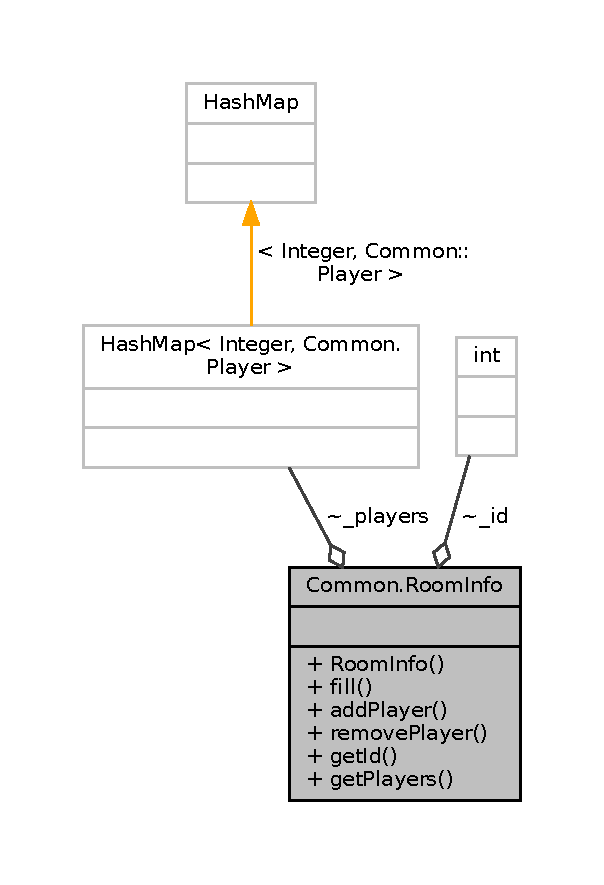
\includegraphics[width=290pt]{classCommon_1_1RoomInfo__coll__graph}
\end{center}
\end{figure}
\subsection*{Public Member Functions}
\begin{DoxyCompactItemize}
\item 
\mbox{\hyperlink{classCommon_1_1RoomInfo_a58cd1b1961ee4539d4cc137760f06332}{Room\+Info}} ()
\item 
\mbox{\hyperlink{classCommon_1_1RoomInfo}{Room\+Info}} \mbox{\hyperlink{classCommon_1_1RoomInfo_ad73d9b718201741f4198b0feeb570f1b}{fill}} (int id)
\item 
void \mbox{\hyperlink{classCommon_1_1RoomInfo_a1681cb7be4e828c16e71285474be9758}{add\+Player}} (\mbox{\hyperlink{classCommon_1_1Player}{Player}} player)
\item 
void \mbox{\hyperlink{classCommon_1_1RoomInfo_ab167bc6ee6568c92d8135622564887b9}{remove\+Player}} (\mbox{\hyperlink{classCommon_1_1Player}{Player}} player)
\item 
int \mbox{\hyperlink{classCommon_1_1RoomInfo_a35582362944dac3d9de2d223f828e90a}{get\+Id}} ()
\item 
Map$<$ Integer, \mbox{\hyperlink{classCommon_1_1Player}{Player}} $>$ \mbox{\hyperlink{classCommon_1_1RoomInfo_a166f72c0cde4165d337f591d68ffe313}{get\+Players}} ()
\end{DoxyCompactItemize}


\subsection{Constructor \& Destructor Documentation}
\mbox{\Hypertarget{classCommon_1_1RoomInfo_a58cd1b1961ee4539d4cc137760f06332}\label{classCommon_1_1RoomInfo_a58cd1b1961ee4539d4cc137760f06332}} 
\index{Common\+::\+Room\+Info@{Common\+::\+Room\+Info}!Room\+Info@{Room\+Info}}
\index{Room\+Info@{Room\+Info}!Common\+::\+Room\+Info@{Common\+::\+Room\+Info}}
\subsubsection{\texorpdfstring{Room\+Info()}{RoomInfo()}}
{\footnotesize\ttfamily Common.\+Room\+Info.\+Room\+Info (\begin{DoxyParamCaption}{ }\end{DoxyParamCaption})\hspace{0.3cm}{\ttfamily [inline]}}



\subsection{Member Function Documentation}
\mbox{\Hypertarget{classCommon_1_1RoomInfo_a1681cb7be4e828c16e71285474be9758}\label{classCommon_1_1RoomInfo_a1681cb7be4e828c16e71285474be9758}} 
\index{Common\+::\+Room\+Info@{Common\+::\+Room\+Info}!add\+Player@{add\+Player}}
\index{add\+Player@{add\+Player}!Common\+::\+Room\+Info@{Common\+::\+Room\+Info}}
\subsubsection{\texorpdfstring{add\+Player()}{addPlayer()}}
{\footnotesize\ttfamily void Common.\+Room\+Info.\+add\+Player (\begin{DoxyParamCaption}\item[{\mbox{\hyperlink{classCommon_1_1Player}{Player}}}]{player }\end{DoxyParamCaption})\hspace{0.3cm}{\ttfamily [inline]}}

\mbox{\Hypertarget{classCommon_1_1RoomInfo_ad73d9b718201741f4198b0feeb570f1b}\label{classCommon_1_1RoomInfo_ad73d9b718201741f4198b0feeb570f1b}} 
\index{Common\+::\+Room\+Info@{Common\+::\+Room\+Info}!fill@{fill}}
\index{fill@{fill}!Common\+::\+Room\+Info@{Common\+::\+Room\+Info}}
\subsubsection{\texorpdfstring{fill()}{fill()}}
{\footnotesize\ttfamily \mbox{\hyperlink{classCommon_1_1RoomInfo}{Room\+Info}} Common.\+Room\+Info.\+fill (\begin{DoxyParamCaption}\item[{int}]{id }\end{DoxyParamCaption})\hspace{0.3cm}{\ttfamily [inline]}}

\mbox{\Hypertarget{classCommon_1_1RoomInfo_a35582362944dac3d9de2d223f828e90a}\label{classCommon_1_1RoomInfo_a35582362944dac3d9de2d223f828e90a}} 
\index{Common\+::\+Room\+Info@{Common\+::\+Room\+Info}!get\+Id@{get\+Id}}
\index{get\+Id@{get\+Id}!Common\+::\+Room\+Info@{Common\+::\+Room\+Info}}
\subsubsection{\texorpdfstring{get\+Id()}{getId()}}
{\footnotesize\ttfamily int Common.\+Room\+Info.\+get\+Id (\begin{DoxyParamCaption}{ }\end{DoxyParamCaption})\hspace{0.3cm}{\ttfamily [inline]}}

\mbox{\Hypertarget{classCommon_1_1RoomInfo_a166f72c0cde4165d337f591d68ffe313}\label{classCommon_1_1RoomInfo_a166f72c0cde4165d337f591d68ffe313}} 
\index{Common\+::\+Room\+Info@{Common\+::\+Room\+Info}!get\+Players@{get\+Players}}
\index{get\+Players@{get\+Players}!Common\+::\+Room\+Info@{Common\+::\+Room\+Info}}
\subsubsection{\texorpdfstring{get\+Players()}{getPlayers()}}
{\footnotesize\ttfamily Map$<$Integer, \mbox{\hyperlink{classCommon_1_1Player}{Player}}$>$ Common.\+Room\+Info.\+get\+Players (\begin{DoxyParamCaption}{ }\end{DoxyParamCaption})\hspace{0.3cm}{\ttfamily [inline]}}

\mbox{\Hypertarget{classCommon_1_1RoomInfo_ab167bc6ee6568c92d8135622564887b9}\label{classCommon_1_1RoomInfo_ab167bc6ee6568c92d8135622564887b9}} 
\index{Common\+::\+Room\+Info@{Common\+::\+Room\+Info}!remove\+Player@{remove\+Player}}
\index{remove\+Player@{remove\+Player}!Common\+::\+Room\+Info@{Common\+::\+Room\+Info}}
\subsubsection{\texorpdfstring{remove\+Player()}{removePlayer()}}
{\footnotesize\ttfamily void Common.\+Room\+Info.\+remove\+Player (\begin{DoxyParamCaption}\item[{\mbox{\hyperlink{classCommon_1_1Player}{Player}}}]{player }\end{DoxyParamCaption})\hspace{0.3cm}{\ttfamily [inline]}}



The documentation for this class was generated from the following file\+:\begin{DoxyCompactItemize}
\item 
/home/tetard/\+Idea\+Projects/j\+Coinche/\+Java\+\_\+jcoinche\+\_\+2017/src/main/java/\+Common/\mbox{\hyperlink{RoomInfo_8java}{Room\+Info.\+java}}\end{DoxyCompactItemize}

\hypertarget{classCommon_1_1RoomListInfo}{}\section{Common.\+Room\+List\+Info Class Reference}
\label{classCommon_1_1RoomListInfo}\index{Common.\+Room\+List\+Info@{Common.\+Room\+List\+Info}}


Collaboration diagram for Common.\+Room\+List\+Info\+:
\nopagebreak
\begin{figure}[H]
\begin{center}
\leavevmode
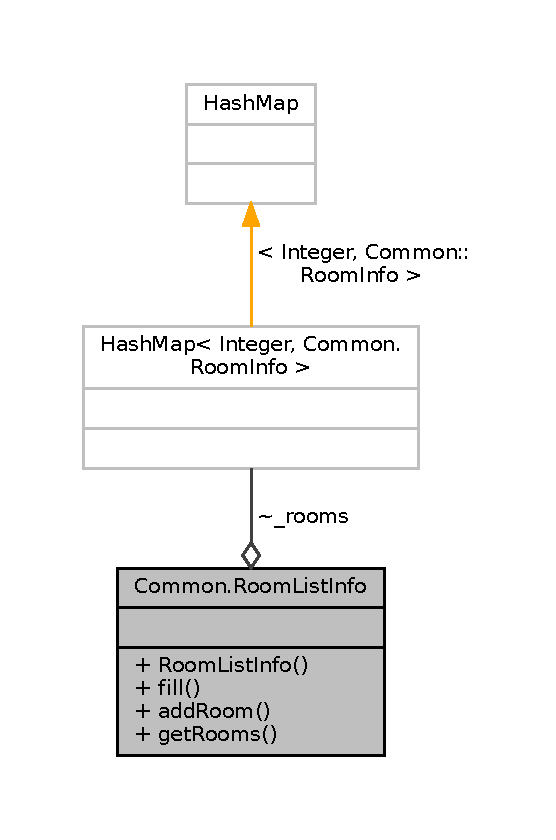
\includegraphics[width=267pt]{classCommon_1_1RoomListInfo__coll__graph}
\end{center}
\end{figure}
\subsection*{Public Member Functions}
\begin{DoxyCompactItemize}
\item 
\mbox{\hyperlink{classCommon_1_1RoomListInfo_a5541213c561f67a7f126c1cd2d70b5ad}{Room\+List\+Info}} ()
\item 
\mbox{\hyperlink{classCommon_1_1RoomListInfo}{Room\+List\+Info}} \mbox{\hyperlink{classCommon_1_1RoomListInfo_a9063826915df8bd9e411df54cca5f6f0}{fill}} (Hash\+Map$<$ Integer, \mbox{\hyperlink{classCommon_1_1RoomInfo}{Room\+Info}} $>$ rooms)
\item 
void \mbox{\hyperlink{classCommon_1_1RoomListInfo_ad177bab88940fd9d3c02d47fe791ce31}{add\+Room}} (\mbox{\hyperlink{classCommon_1_1RoomInfo}{Room\+Info}} room)
\item 
Hash\+Map$<$ Integer, \mbox{\hyperlink{classCommon_1_1RoomInfo}{Room\+Info}} $>$ \mbox{\hyperlink{classCommon_1_1RoomListInfo_a2546f4c16f204de286beae2528c2ea51}{get\+Rooms}} ()
\end{DoxyCompactItemize}


\subsection{Constructor \& Destructor Documentation}
\mbox{\Hypertarget{classCommon_1_1RoomListInfo_a5541213c561f67a7f126c1cd2d70b5ad}\label{classCommon_1_1RoomListInfo_a5541213c561f67a7f126c1cd2d70b5ad}} 
\index{Common\+::\+Room\+List\+Info@{Common\+::\+Room\+List\+Info}!Room\+List\+Info@{Room\+List\+Info}}
\index{Room\+List\+Info@{Room\+List\+Info}!Common\+::\+Room\+List\+Info@{Common\+::\+Room\+List\+Info}}
\subsubsection{\texorpdfstring{Room\+List\+Info()}{RoomListInfo()}}
{\footnotesize\ttfamily Common.\+Room\+List\+Info.\+Room\+List\+Info (\begin{DoxyParamCaption}{ }\end{DoxyParamCaption})\hspace{0.3cm}{\ttfamily [inline]}}



\subsection{Member Function Documentation}
\mbox{\Hypertarget{classCommon_1_1RoomListInfo_ad177bab88940fd9d3c02d47fe791ce31}\label{classCommon_1_1RoomListInfo_ad177bab88940fd9d3c02d47fe791ce31}} 
\index{Common\+::\+Room\+List\+Info@{Common\+::\+Room\+List\+Info}!add\+Room@{add\+Room}}
\index{add\+Room@{add\+Room}!Common\+::\+Room\+List\+Info@{Common\+::\+Room\+List\+Info}}
\subsubsection{\texorpdfstring{add\+Room()}{addRoom()}}
{\footnotesize\ttfamily void Common.\+Room\+List\+Info.\+add\+Room (\begin{DoxyParamCaption}\item[{\mbox{\hyperlink{classCommon_1_1RoomInfo}{Room\+Info}}}]{room }\end{DoxyParamCaption})\hspace{0.3cm}{\ttfamily [inline]}}

\mbox{\Hypertarget{classCommon_1_1RoomListInfo_a9063826915df8bd9e411df54cca5f6f0}\label{classCommon_1_1RoomListInfo_a9063826915df8bd9e411df54cca5f6f0}} 
\index{Common\+::\+Room\+List\+Info@{Common\+::\+Room\+List\+Info}!fill@{fill}}
\index{fill@{fill}!Common\+::\+Room\+List\+Info@{Common\+::\+Room\+List\+Info}}
\subsubsection{\texorpdfstring{fill()}{fill()}}
{\footnotesize\ttfamily \mbox{\hyperlink{classCommon_1_1RoomListInfo}{Room\+List\+Info}} Common.\+Room\+List\+Info.\+fill (\begin{DoxyParamCaption}\item[{Hash\+Map$<$ Integer, \mbox{\hyperlink{classCommon_1_1RoomInfo}{Room\+Info}} $>$}]{rooms }\end{DoxyParamCaption})\hspace{0.3cm}{\ttfamily [inline]}}

\mbox{\Hypertarget{classCommon_1_1RoomListInfo_a2546f4c16f204de286beae2528c2ea51}\label{classCommon_1_1RoomListInfo_a2546f4c16f204de286beae2528c2ea51}} 
\index{Common\+::\+Room\+List\+Info@{Common\+::\+Room\+List\+Info}!get\+Rooms@{get\+Rooms}}
\index{get\+Rooms@{get\+Rooms}!Common\+::\+Room\+List\+Info@{Common\+::\+Room\+List\+Info}}
\subsubsection{\texorpdfstring{get\+Rooms()}{getRooms()}}
{\footnotesize\ttfamily Hash\+Map$<$Integer, \mbox{\hyperlink{classCommon_1_1RoomInfo}{Room\+Info}}$>$ Common.\+Room\+List\+Info.\+get\+Rooms (\begin{DoxyParamCaption}{ }\end{DoxyParamCaption})\hspace{0.3cm}{\ttfamily [inline]}}



The documentation for this class was generated from the following file\+:\begin{DoxyCompactItemize}
\item 
/home/tetard/\+Idea\+Projects/j\+Coinche/\+Java\+\_\+jcoinche\+\_\+2017/src/main/java/\+Common/\mbox{\hyperlink{RoomListInfo_8java}{Room\+List\+Info.\+java}}\end{DoxyCompactItemize}

\hypertarget{classClient_1_1Model_1_1RoomListModel}{}\section{Client.\+Model.\+Room\+List\+Model Class Reference}
\label{classClient_1_1Model_1_1RoomListModel}\index{Client.\+Model.\+Room\+List\+Model@{Client.\+Model.\+Room\+List\+Model}}


Inheritance diagram for Client.\+Model.\+Room\+List\+Model\+:
\nopagebreak
\begin{figure}[H]
\begin{center}
\leavevmode
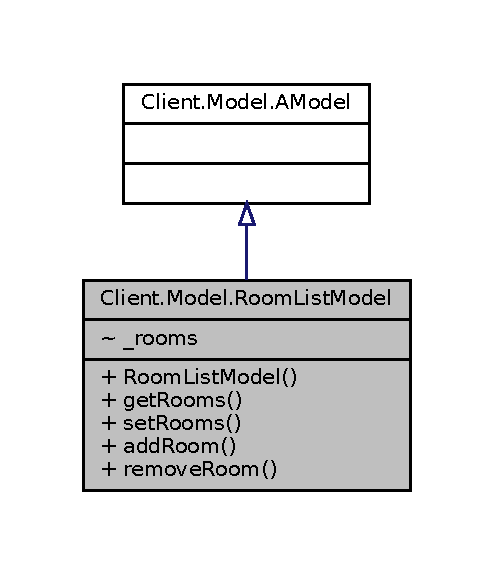
\includegraphics[width=237pt]{classClient_1_1Model_1_1RoomListModel__inherit__graph}
\end{center}
\end{figure}


Collaboration diagram for Client.\+Model.\+Room\+List\+Model\+:
\nopagebreak
\begin{figure}[H]
\begin{center}
\leavevmode
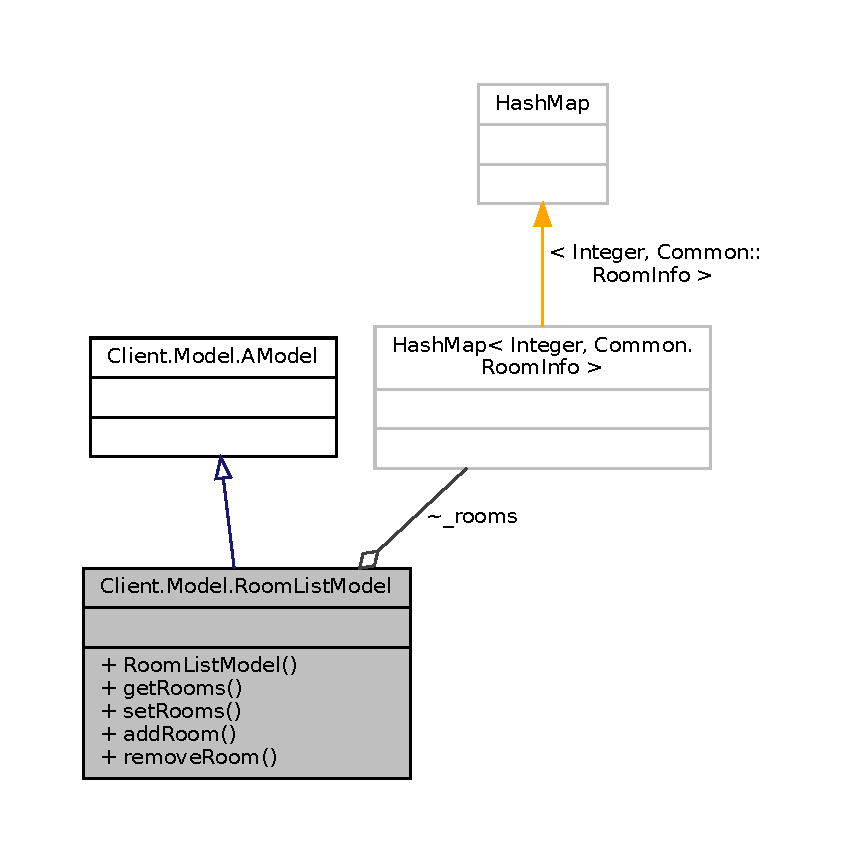
\includegraphics[width=350pt]{classClient_1_1Model_1_1RoomListModel__coll__graph}
\end{center}
\end{figure}
\subsection*{Public Member Functions}
\begin{DoxyCompactItemize}
\item 
\mbox{\hyperlink{classClient_1_1Model_1_1RoomListModel_a1738a460af89d76a66bd9c62651d5d6e}{Room\+List\+Model}} ()
\item 
Hash\+Map$<$ Integer, \mbox{\hyperlink{classCommon_1_1RoomInfo}{Room\+Info}} $>$ \mbox{\hyperlink{classClient_1_1Model_1_1RoomListModel_a10a966393e0d06de3742a372023f5ff3}{get\+Rooms}} ()
\item 
void \mbox{\hyperlink{classClient_1_1Model_1_1RoomListModel_a1927f5b273c8b47f2e9f72fe7480b8a0}{set\+Rooms}} (Hash\+Map$<$ Integer, \mbox{\hyperlink{classCommon_1_1RoomInfo}{Room\+Info}} $>$ rooms)
\item 
void \mbox{\hyperlink{classClient_1_1Model_1_1RoomListModel_ae57d201334439d5a28c8f6e889d91a7f}{add\+Room}} (\mbox{\hyperlink{classCommon_1_1RoomInfo}{Room\+Info}} room)
\item 
void \mbox{\hyperlink{classClient_1_1Model_1_1RoomListModel_a73e2d5942607d4a014a96c74adaa7f2e}{remove\+Room}} (int id)
\end{DoxyCompactItemize}


\subsection{Constructor \& Destructor Documentation}
\mbox{\Hypertarget{classClient_1_1Model_1_1RoomListModel_a1738a460af89d76a66bd9c62651d5d6e}\label{classClient_1_1Model_1_1RoomListModel_a1738a460af89d76a66bd9c62651d5d6e}} 
\index{Client\+::\+Model\+::\+Room\+List\+Model@{Client\+::\+Model\+::\+Room\+List\+Model}!Room\+List\+Model@{Room\+List\+Model}}
\index{Room\+List\+Model@{Room\+List\+Model}!Client\+::\+Model\+::\+Room\+List\+Model@{Client\+::\+Model\+::\+Room\+List\+Model}}
\subsubsection{\texorpdfstring{Room\+List\+Model()}{RoomListModel()}}
{\footnotesize\ttfamily Client.\+Model.\+Room\+List\+Model.\+Room\+List\+Model (\begin{DoxyParamCaption}{ }\end{DoxyParamCaption})\hspace{0.3cm}{\ttfamily [inline]}}



\subsection{Member Function Documentation}
\mbox{\Hypertarget{classClient_1_1Model_1_1RoomListModel_ae57d201334439d5a28c8f6e889d91a7f}\label{classClient_1_1Model_1_1RoomListModel_ae57d201334439d5a28c8f6e889d91a7f}} 
\index{Client\+::\+Model\+::\+Room\+List\+Model@{Client\+::\+Model\+::\+Room\+List\+Model}!add\+Room@{add\+Room}}
\index{add\+Room@{add\+Room}!Client\+::\+Model\+::\+Room\+List\+Model@{Client\+::\+Model\+::\+Room\+List\+Model}}
\subsubsection{\texorpdfstring{add\+Room()}{addRoom()}}
{\footnotesize\ttfamily void Client.\+Model.\+Room\+List\+Model.\+add\+Room (\begin{DoxyParamCaption}\item[{\mbox{\hyperlink{classCommon_1_1RoomInfo}{Room\+Info}}}]{room }\end{DoxyParamCaption})\hspace{0.3cm}{\ttfamily [inline]}}

\mbox{\Hypertarget{classClient_1_1Model_1_1RoomListModel_a10a966393e0d06de3742a372023f5ff3}\label{classClient_1_1Model_1_1RoomListModel_a10a966393e0d06de3742a372023f5ff3}} 
\index{Client\+::\+Model\+::\+Room\+List\+Model@{Client\+::\+Model\+::\+Room\+List\+Model}!get\+Rooms@{get\+Rooms}}
\index{get\+Rooms@{get\+Rooms}!Client\+::\+Model\+::\+Room\+List\+Model@{Client\+::\+Model\+::\+Room\+List\+Model}}
\subsubsection{\texorpdfstring{get\+Rooms()}{getRooms()}}
{\footnotesize\ttfamily Hash\+Map$<$Integer, \mbox{\hyperlink{classCommon_1_1RoomInfo}{Room\+Info}}$>$ Client.\+Model.\+Room\+List\+Model.\+get\+Rooms (\begin{DoxyParamCaption}{ }\end{DoxyParamCaption})\hspace{0.3cm}{\ttfamily [inline]}}

\mbox{\Hypertarget{classClient_1_1Model_1_1RoomListModel_a73e2d5942607d4a014a96c74adaa7f2e}\label{classClient_1_1Model_1_1RoomListModel_a73e2d5942607d4a014a96c74adaa7f2e}} 
\index{Client\+::\+Model\+::\+Room\+List\+Model@{Client\+::\+Model\+::\+Room\+List\+Model}!remove\+Room@{remove\+Room}}
\index{remove\+Room@{remove\+Room}!Client\+::\+Model\+::\+Room\+List\+Model@{Client\+::\+Model\+::\+Room\+List\+Model}}
\subsubsection{\texorpdfstring{remove\+Room()}{removeRoom()}}
{\footnotesize\ttfamily void Client.\+Model.\+Room\+List\+Model.\+remove\+Room (\begin{DoxyParamCaption}\item[{int}]{id }\end{DoxyParamCaption})\hspace{0.3cm}{\ttfamily [inline]}}

\mbox{\Hypertarget{classClient_1_1Model_1_1RoomListModel_a1927f5b273c8b47f2e9f72fe7480b8a0}\label{classClient_1_1Model_1_1RoomListModel_a1927f5b273c8b47f2e9f72fe7480b8a0}} 
\index{Client\+::\+Model\+::\+Room\+List\+Model@{Client\+::\+Model\+::\+Room\+List\+Model}!set\+Rooms@{set\+Rooms}}
\index{set\+Rooms@{set\+Rooms}!Client\+::\+Model\+::\+Room\+List\+Model@{Client\+::\+Model\+::\+Room\+List\+Model}}
\subsubsection{\texorpdfstring{set\+Rooms()}{setRooms()}}
{\footnotesize\ttfamily void Client.\+Model.\+Room\+List\+Model.\+set\+Rooms (\begin{DoxyParamCaption}\item[{Hash\+Map$<$ Integer, \mbox{\hyperlink{classCommon_1_1RoomInfo}{Room\+Info}} $>$}]{rooms }\end{DoxyParamCaption})\hspace{0.3cm}{\ttfamily [inline]}}



The documentation for this class was generated from the following file\+:\begin{DoxyCompactItemize}
\item 
/home/tetard/\+Idea\+Projects/j\+Coinche/\+Java\+\_\+jcoinche\+\_\+2017/src/main/java/\+Client/\+Model/\mbox{\hyperlink{RoomListModel_8java}{Room\+List\+Model.\+java}}\end{DoxyCompactItemize}

\hypertarget{classCommon_1_1RoomMovingClient}{}\section{Common.\+Room\+Moving\+Client Class Reference}
\label{classCommon_1_1RoomMovingClient}\index{Common.\+Room\+Moving\+Client@{Common.\+Room\+Moving\+Client}}


Collaboration diagram for Common.\+Room\+Moving\+Client\+:
\nopagebreak
\begin{figure}[H]
\begin{center}
\leavevmode
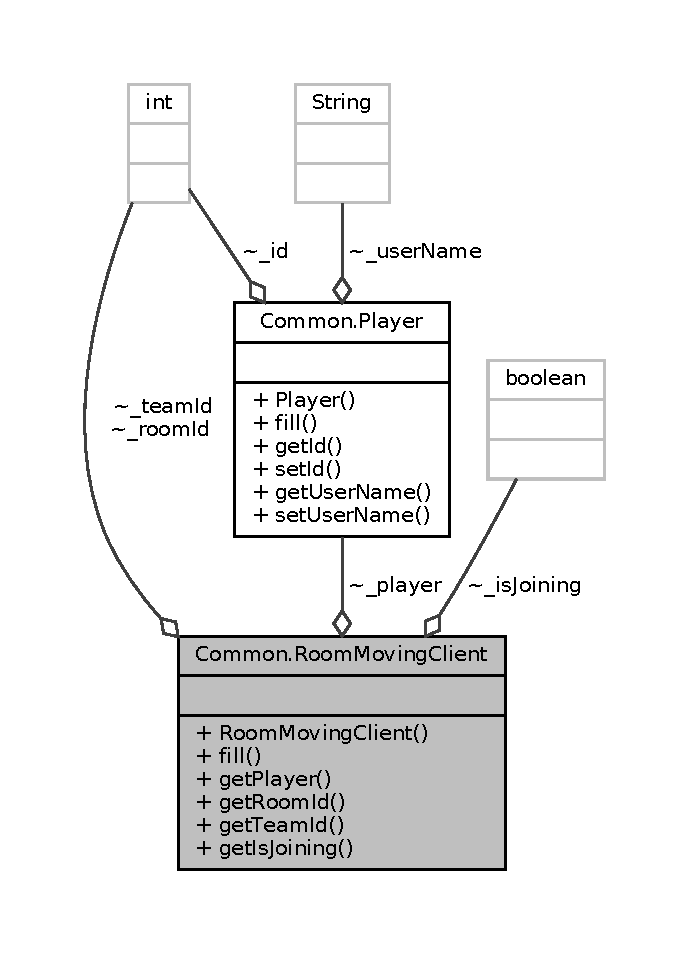
\includegraphics[width=330pt]{classCommon_1_1RoomMovingClient__coll__graph}
\end{center}
\end{figure}
\subsection*{Public Member Functions}
\begin{DoxyCompactItemize}
\item 
\mbox{\hyperlink{classCommon_1_1RoomMovingClient_a447754b3da2c6ac8cd32b2a6f490ef6c}{Room\+Moving\+Client}} ()
\item 
\mbox{\hyperlink{classCommon_1_1RoomMovingClient}{Room\+Moving\+Client}} \mbox{\hyperlink{classCommon_1_1RoomMovingClient_a4bb429f47a0b7574d223bbe63aaeb096}{fill}} (\mbox{\hyperlink{classCommon_1_1Player}{Player}} player, int room\+Id, boolean is\+Joining, int team\+Id)
\item 
\mbox{\hyperlink{classCommon_1_1Player}{Player}} \mbox{\hyperlink{classCommon_1_1RoomMovingClient_a7e9f5ba38fba3138d8b7438be1a834f0}{get\+Player}} ()
\item 
int \mbox{\hyperlink{classCommon_1_1RoomMovingClient_a81d463606183e832672ec00b25c07088}{get\+Room\+Id}} ()
\item 
int \mbox{\hyperlink{classCommon_1_1RoomMovingClient_afdc28b796ecc99d62049c98fb53cef72}{get\+Team\+Id}} ()
\item 
boolean \mbox{\hyperlink{classCommon_1_1RoomMovingClient_a386ca7363315be9857c0c841d41d13a1}{get\+Is\+Joining}} ()
\end{DoxyCompactItemize}


\subsection{Constructor \& Destructor Documentation}
\mbox{\Hypertarget{classCommon_1_1RoomMovingClient_a447754b3da2c6ac8cd32b2a6f490ef6c}\label{classCommon_1_1RoomMovingClient_a447754b3da2c6ac8cd32b2a6f490ef6c}} 
\index{Common\+::\+Room\+Moving\+Client@{Common\+::\+Room\+Moving\+Client}!Room\+Moving\+Client@{Room\+Moving\+Client}}
\index{Room\+Moving\+Client@{Room\+Moving\+Client}!Common\+::\+Room\+Moving\+Client@{Common\+::\+Room\+Moving\+Client}}
\subsubsection{\texorpdfstring{Room\+Moving\+Client()}{RoomMovingClient()}}
{\footnotesize\ttfamily Common.\+Room\+Moving\+Client.\+Room\+Moving\+Client (\begin{DoxyParamCaption}{ }\end{DoxyParamCaption})\hspace{0.3cm}{\ttfamily [inline]}}



\subsection{Member Function Documentation}
\mbox{\Hypertarget{classCommon_1_1RoomMovingClient_a4bb429f47a0b7574d223bbe63aaeb096}\label{classCommon_1_1RoomMovingClient_a4bb429f47a0b7574d223bbe63aaeb096}} 
\index{Common\+::\+Room\+Moving\+Client@{Common\+::\+Room\+Moving\+Client}!fill@{fill}}
\index{fill@{fill}!Common\+::\+Room\+Moving\+Client@{Common\+::\+Room\+Moving\+Client}}
\subsubsection{\texorpdfstring{fill()}{fill()}}
{\footnotesize\ttfamily \mbox{\hyperlink{classCommon_1_1RoomMovingClient}{Room\+Moving\+Client}} Common.\+Room\+Moving\+Client.\+fill (\begin{DoxyParamCaption}\item[{\mbox{\hyperlink{classCommon_1_1Player}{Player}}}]{player,  }\item[{int}]{room\+Id,  }\item[{boolean}]{is\+Joining,  }\item[{int}]{team\+Id }\end{DoxyParamCaption})\hspace{0.3cm}{\ttfamily [inline]}}

\mbox{\Hypertarget{classCommon_1_1RoomMovingClient_a386ca7363315be9857c0c841d41d13a1}\label{classCommon_1_1RoomMovingClient_a386ca7363315be9857c0c841d41d13a1}} 
\index{Common\+::\+Room\+Moving\+Client@{Common\+::\+Room\+Moving\+Client}!get\+Is\+Joining@{get\+Is\+Joining}}
\index{get\+Is\+Joining@{get\+Is\+Joining}!Common\+::\+Room\+Moving\+Client@{Common\+::\+Room\+Moving\+Client}}
\subsubsection{\texorpdfstring{get\+Is\+Joining()}{getIsJoining()}}
{\footnotesize\ttfamily boolean Common.\+Room\+Moving\+Client.\+get\+Is\+Joining (\begin{DoxyParamCaption}{ }\end{DoxyParamCaption})\hspace{0.3cm}{\ttfamily [inline]}}

\mbox{\Hypertarget{classCommon_1_1RoomMovingClient_a7e9f5ba38fba3138d8b7438be1a834f0}\label{classCommon_1_1RoomMovingClient_a7e9f5ba38fba3138d8b7438be1a834f0}} 
\index{Common\+::\+Room\+Moving\+Client@{Common\+::\+Room\+Moving\+Client}!get\+Player@{get\+Player}}
\index{get\+Player@{get\+Player}!Common\+::\+Room\+Moving\+Client@{Common\+::\+Room\+Moving\+Client}}
\subsubsection{\texorpdfstring{get\+Player()}{getPlayer()}}
{\footnotesize\ttfamily \mbox{\hyperlink{classCommon_1_1Player}{Player}} Common.\+Room\+Moving\+Client.\+get\+Player (\begin{DoxyParamCaption}{ }\end{DoxyParamCaption})\hspace{0.3cm}{\ttfamily [inline]}}

\mbox{\Hypertarget{classCommon_1_1RoomMovingClient_a81d463606183e832672ec00b25c07088}\label{classCommon_1_1RoomMovingClient_a81d463606183e832672ec00b25c07088}} 
\index{Common\+::\+Room\+Moving\+Client@{Common\+::\+Room\+Moving\+Client}!get\+Room\+Id@{get\+Room\+Id}}
\index{get\+Room\+Id@{get\+Room\+Id}!Common\+::\+Room\+Moving\+Client@{Common\+::\+Room\+Moving\+Client}}
\subsubsection{\texorpdfstring{get\+Room\+Id()}{getRoomId()}}
{\footnotesize\ttfamily int Common.\+Room\+Moving\+Client.\+get\+Room\+Id (\begin{DoxyParamCaption}{ }\end{DoxyParamCaption})\hspace{0.3cm}{\ttfamily [inline]}}

\mbox{\Hypertarget{classCommon_1_1RoomMovingClient_afdc28b796ecc99d62049c98fb53cef72}\label{classCommon_1_1RoomMovingClient_afdc28b796ecc99d62049c98fb53cef72}} 
\index{Common\+::\+Room\+Moving\+Client@{Common\+::\+Room\+Moving\+Client}!get\+Team\+Id@{get\+Team\+Id}}
\index{get\+Team\+Id@{get\+Team\+Id}!Common\+::\+Room\+Moving\+Client@{Common\+::\+Room\+Moving\+Client}}
\subsubsection{\texorpdfstring{get\+Team\+Id()}{getTeamId()}}
{\footnotesize\ttfamily int Common.\+Room\+Moving\+Client.\+get\+Team\+Id (\begin{DoxyParamCaption}{ }\end{DoxyParamCaption})\hspace{0.3cm}{\ttfamily [inline]}}



The documentation for this class was generated from the following file\+:\begin{DoxyCompactItemize}
\item 
/home/tetard/\+Idea\+Projects/j\+Coinche/\+Java\+\_\+jcoinche\+\_\+2017/src/main/java/\+Common/\mbox{\hyperlink{RoomMovingClient_8java}{Room\+Moving\+Client.\+java}}\end{DoxyCompactItemize}

\hypertarget{classClient_1_1Model_1_1Score}{}\section{Client.\+Model.\+Score Class Reference}
\label{classClient_1_1Model_1_1Score}\index{Client.\+Model.\+Score@{Client.\+Model.\+Score}}


Collaboration diagram for Client.\+Model.\+Score\+:
\nopagebreak
\begin{figure}[H]
\begin{center}
\leavevmode
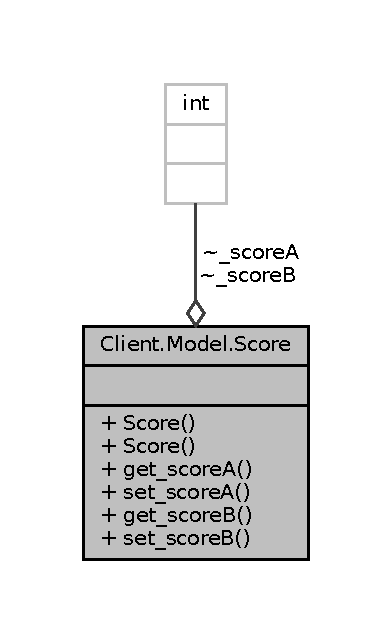
\includegraphics[width=188pt]{classClient_1_1Model_1_1Score__coll__graph}
\end{center}
\end{figure}
\subsection*{Public Member Functions}
\begin{DoxyCompactItemize}
\item 
\mbox{\hyperlink{classClient_1_1Model_1_1Score_a74a6c9f28cfb3bcc6e7f6e29bf627009}{Score}} (int a, int b)
\item 
\mbox{\hyperlink{classClient_1_1Model_1_1Score_ab469f2ace75be01b2eda077e15e753b7}{Score}} ()
\item 
int \mbox{\hyperlink{classClient_1_1Model_1_1Score_a8fb4e69a2eb1ec879cab4cf4bb017f9b}{get\+\_\+scoreA}} ()
\item 
void \mbox{\hyperlink{classClient_1_1Model_1_1Score_a53eea45adc659276ed4a521c8244e763}{set\+\_\+scoreA}} (int scoreA)
\item 
int \mbox{\hyperlink{classClient_1_1Model_1_1Score_a26810cd9664942d722198c892866f4b7}{get\+\_\+scoreB}} ()
\item 
void \mbox{\hyperlink{classClient_1_1Model_1_1Score_a2090cd988d6f53fc05637ed59aa7b3b1}{set\+\_\+scoreB}} (int scoreB)
\end{DoxyCompactItemize}


\subsection{Constructor \& Destructor Documentation}
\mbox{\Hypertarget{classClient_1_1Model_1_1Score_a74a6c9f28cfb3bcc6e7f6e29bf627009}\label{classClient_1_1Model_1_1Score_a74a6c9f28cfb3bcc6e7f6e29bf627009}} 
\index{Client\+::\+Model\+::\+Score@{Client\+::\+Model\+::\+Score}!Score@{Score}}
\index{Score@{Score}!Client\+::\+Model\+::\+Score@{Client\+::\+Model\+::\+Score}}
\subsubsection{\texorpdfstring{Score()}{Score()}\hspace{0.1cm}{\footnotesize\ttfamily [1/2]}}
{\footnotesize\ttfamily Client.\+Model.\+Score.\+Score (\begin{DoxyParamCaption}\item[{int}]{a,  }\item[{int}]{b }\end{DoxyParamCaption})\hspace{0.3cm}{\ttfamily [inline]}}

\mbox{\Hypertarget{classClient_1_1Model_1_1Score_ab469f2ace75be01b2eda077e15e753b7}\label{classClient_1_1Model_1_1Score_ab469f2ace75be01b2eda077e15e753b7}} 
\index{Client\+::\+Model\+::\+Score@{Client\+::\+Model\+::\+Score}!Score@{Score}}
\index{Score@{Score}!Client\+::\+Model\+::\+Score@{Client\+::\+Model\+::\+Score}}
\subsubsection{\texorpdfstring{Score()}{Score()}\hspace{0.1cm}{\footnotesize\ttfamily [2/2]}}
{\footnotesize\ttfamily Client.\+Model.\+Score.\+Score (\begin{DoxyParamCaption}{ }\end{DoxyParamCaption})\hspace{0.3cm}{\ttfamily [inline]}}



\subsection{Member Function Documentation}
\mbox{\Hypertarget{classClient_1_1Model_1_1Score_a8fb4e69a2eb1ec879cab4cf4bb017f9b}\label{classClient_1_1Model_1_1Score_a8fb4e69a2eb1ec879cab4cf4bb017f9b}} 
\index{Client\+::\+Model\+::\+Score@{Client\+::\+Model\+::\+Score}!get\+\_\+scoreA@{get\+\_\+scoreA}}
\index{get\+\_\+scoreA@{get\+\_\+scoreA}!Client\+::\+Model\+::\+Score@{Client\+::\+Model\+::\+Score}}
\subsubsection{\texorpdfstring{get\+\_\+score\+A()}{get\_scoreA()}}
{\footnotesize\ttfamily int Client.\+Model.\+Score.\+get\+\_\+scoreA (\begin{DoxyParamCaption}{ }\end{DoxyParamCaption})\hspace{0.3cm}{\ttfamily [inline]}}

\mbox{\Hypertarget{classClient_1_1Model_1_1Score_a26810cd9664942d722198c892866f4b7}\label{classClient_1_1Model_1_1Score_a26810cd9664942d722198c892866f4b7}} 
\index{Client\+::\+Model\+::\+Score@{Client\+::\+Model\+::\+Score}!get\+\_\+scoreB@{get\+\_\+scoreB}}
\index{get\+\_\+scoreB@{get\+\_\+scoreB}!Client\+::\+Model\+::\+Score@{Client\+::\+Model\+::\+Score}}
\subsubsection{\texorpdfstring{get\+\_\+score\+B()}{get\_scoreB()}}
{\footnotesize\ttfamily int Client.\+Model.\+Score.\+get\+\_\+scoreB (\begin{DoxyParamCaption}{ }\end{DoxyParamCaption})\hspace{0.3cm}{\ttfamily [inline]}}

\mbox{\Hypertarget{classClient_1_1Model_1_1Score_a53eea45adc659276ed4a521c8244e763}\label{classClient_1_1Model_1_1Score_a53eea45adc659276ed4a521c8244e763}} 
\index{Client\+::\+Model\+::\+Score@{Client\+::\+Model\+::\+Score}!set\+\_\+scoreA@{set\+\_\+scoreA}}
\index{set\+\_\+scoreA@{set\+\_\+scoreA}!Client\+::\+Model\+::\+Score@{Client\+::\+Model\+::\+Score}}
\subsubsection{\texorpdfstring{set\+\_\+score\+A()}{set\_scoreA()}}
{\footnotesize\ttfamily void Client.\+Model.\+Score.\+set\+\_\+scoreA (\begin{DoxyParamCaption}\item[{int}]{scoreA }\end{DoxyParamCaption})\hspace{0.3cm}{\ttfamily [inline]}}

\mbox{\Hypertarget{classClient_1_1Model_1_1Score_a2090cd988d6f53fc05637ed59aa7b3b1}\label{classClient_1_1Model_1_1Score_a2090cd988d6f53fc05637ed59aa7b3b1}} 
\index{Client\+::\+Model\+::\+Score@{Client\+::\+Model\+::\+Score}!set\+\_\+scoreB@{set\+\_\+scoreB}}
\index{set\+\_\+scoreB@{set\+\_\+scoreB}!Client\+::\+Model\+::\+Score@{Client\+::\+Model\+::\+Score}}
\subsubsection{\texorpdfstring{set\+\_\+score\+B()}{set\_scoreB()}}
{\footnotesize\ttfamily void Client.\+Model.\+Score.\+set\+\_\+scoreB (\begin{DoxyParamCaption}\item[{int}]{scoreB }\end{DoxyParamCaption})\hspace{0.3cm}{\ttfamily [inline]}}



The documentation for this class was generated from the following file\+:\begin{DoxyCompactItemize}
\item 
/home/tetard/\+Idea\+Projects/j\+Coinche/\+Java\+\_\+jcoinche\+\_\+2017/src/main/java/\+Client/\+Model/\mbox{\hyperlink{Score_8java}{Score.\+java}}\end{DoxyCompactItemize}

\hypertarget{classCommon_1_1SendCardToPlayer}{}\section{Common.\+Send\+Card\+To\+Player Class Reference}
\label{classCommon_1_1SendCardToPlayer}\index{Common.\+Send\+Card\+To\+Player@{Common.\+Send\+Card\+To\+Player}}


Collaboration diagram for Common.\+Send\+Card\+To\+Player\+:
\nopagebreak
\begin{figure}[H]
\begin{center}
\leavevmode
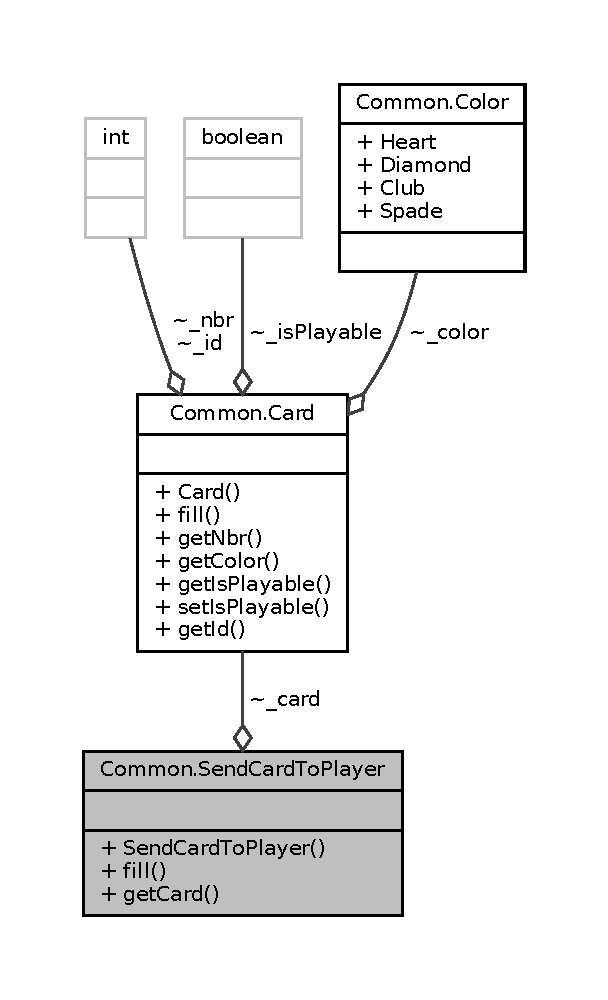
\includegraphics[width=292pt]{classCommon_1_1SendCardToPlayer__coll__graph}
\end{center}
\end{figure}
\subsection*{Public Member Functions}
\begin{DoxyCompactItemize}
\item 
\mbox{\hyperlink{classCommon_1_1SendCardToPlayer_abb4ae3f97446d7b5bf4c54d2cfb095b0}{Send\+Card\+To\+Player}} ()
\item 
\mbox{\hyperlink{classCommon_1_1SendCardToPlayer}{Send\+Card\+To\+Player}} \mbox{\hyperlink{classCommon_1_1SendCardToPlayer_aaf5d1cdf5516599d15f7f0888eb9500a}{fill}} (\mbox{\hyperlink{classCommon_1_1Card}{Card}} card)
\item 
\mbox{\hyperlink{classCommon_1_1Card}{Card}} \mbox{\hyperlink{classCommon_1_1SendCardToPlayer_a63b0f14afc271a12b147caf267a52e23}{get\+Card}} ()
\end{DoxyCompactItemize}


\subsection{Constructor \& Destructor Documentation}
\mbox{\Hypertarget{classCommon_1_1SendCardToPlayer_abb4ae3f97446d7b5bf4c54d2cfb095b0}\label{classCommon_1_1SendCardToPlayer_abb4ae3f97446d7b5bf4c54d2cfb095b0}} 
\index{Common\+::\+Send\+Card\+To\+Player@{Common\+::\+Send\+Card\+To\+Player}!Send\+Card\+To\+Player@{Send\+Card\+To\+Player}}
\index{Send\+Card\+To\+Player@{Send\+Card\+To\+Player}!Common\+::\+Send\+Card\+To\+Player@{Common\+::\+Send\+Card\+To\+Player}}
\subsubsection{\texorpdfstring{Send\+Card\+To\+Player()}{SendCardToPlayer()}}
{\footnotesize\ttfamily Common.\+Send\+Card\+To\+Player.\+Send\+Card\+To\+Player (\begin{DoxyParamCaption}{ }\end{DoxyParamCaption})\hspace{0.3cm}{\ttfamily [inline]}}



\subsection{Member Function Documentation}
\mbox{\Hypertarget{classCommon_1_1SendCardToPlayer_aaf5d1cdf5516599d15f7f0888eb9500a}\label{classCommon_1_1SendCardToPlayer_aaf5d1cdf5516599d15f7f0888eb9500a}} 
\index{Common\+::\+Send\+Card\+To\+Player@{Common\+::\+Send\+Card\+To\+Player}!fill@{fill}}
\index{fill@{fill}!Common\+::\+Send\+Card\+To\+Player@{Common\+::\+Send\+Card\+To\+Player}}
\subsubsection{\texorpdfstring{fill()}{fill()}}
{\footnotesize\ttfamily \mbox{\hyperlink{classCommon_1_1SendCardToPlayer}{Send\+Card\+To\+Player}} Common.\+Send\+Card\+To\+Player.\+fill (\begin{DoxyParamCaption}\item[{\mbox{\hyperlink{classCommon_1_1Card}{Card}}}]{card }\end{DoxyParamCaption})\hspace{0.3cm}{\ttfamily [inline]}}

\mbox{\Hypertarget{classCommon_1_1SendCardToPlayer_a63b0f14afc271a12b147caf267a52e23}\label{classCommon_1_1SendCardToPlayer_a63b0f14afc271a12b147caf267a52e23}} 
\index{Common\+::\+Send\+Card\+To\+Player@{Common\+::\+Send\+Card\+To\+Player}!get\+Card@{get\+Card}}
\index{get\+Card@{get\+Card}!Common\+::\+Send\+Card\+To\+Player@{Common\+::\+Send\+Card\+To\+Player}}
\subsubsection{\texorpdfstring{get\+Card()}{getCard()}}
{\footnotesize\ttfamily \mbox{\hyperlink{classCommon_1_1Card}{Card}} Common.\+Send\+Card\+To\+Player.\+get\+Card (\begin{DoxyParamCaption}{ }\end{DoxyParamCaption})\hspace{0.3cm}{\ttfamily [inline]}}



The documentation for this class was generated from the following file\+:\begin{DoxyCompactItemize}
\item 
/home/tetard/\+Idea\+Projects/j\+Coinche/\+Java\+\_\+jcoinche\+\_\+2017/src/main/java/\+Common/\mbox{\hyperlink{SendCardToPlayer_8java}{Send\+Card\+To\+Player.\+java}}\end{DoxyCompactItemize}

\hypertarget{classCommon_1_1TeamAttribution}{}\section{Common.\+Team\+Attribution Class Reference}
\label{classCommon_1_1TeamAttribution}\index{Common.\+Team\+Attribution@{Common.\+Team\+Attribution}}


Collaboration diagram for Common.\+Team\+Attribution\+:
\nopagebreak
\begin{figure}[H]
\begin{center}
\leavevmode
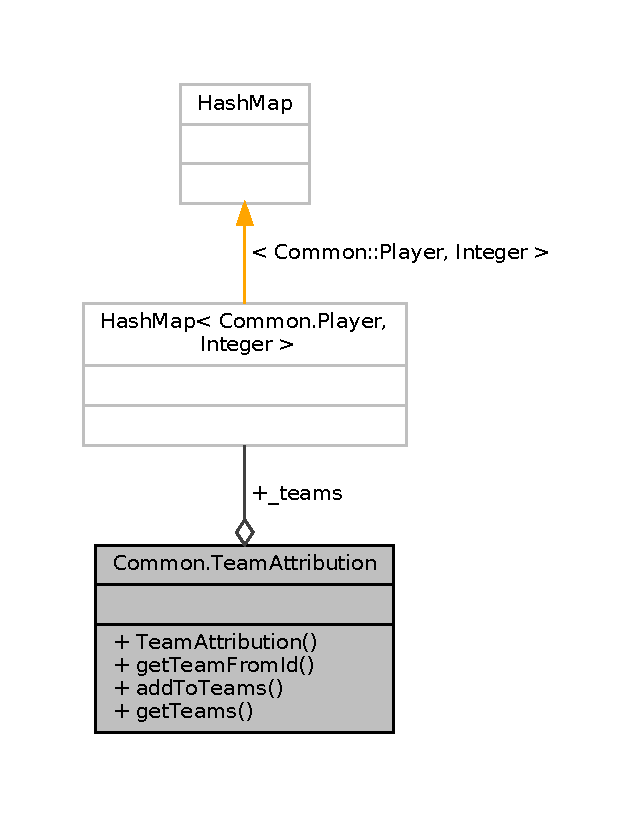
\includegraphics[width=306pt]{classCommon_1_1TeamAttribution__coll__graph}
\end{center}
\end{figure}
\subsection*{Public Member Functions}
\begin{DoxyCompactItemize}
\item 
\mbox{\hyperlink{classCommon_1_1TeamAttribution_ae9e3f8d680bd877d243b2bd1261e915f}{Team\+Attribution}} ()
\item 
int \mbox{\hyperlink{classCommon_1_1TeamAttribution_a4dc4bc10ccb136c5859a29210dca6115}{get\+Team\+From\+Id}} (int id)
\item 
void \mbox{\hyperlink{classCommon_1_1TeamAttribution_aa21f38f5bb27527934d518ea68120f56}{add\+To\+Teams}} (\mbox{\hyperlink{classCommon_1_1Player}{Player}} player, int team)
\item 
Hash\+Map$<$ \mbox{\hyperlink{classCommon_1_1Player}{Player}}, Integer $>$ \mbox{\hyperlink{classCommon_1_1TeamAttribution_ae2b14573fa95f73bf00ca7df017a9b2c}{get\+Teams}} ()
\end{DoxyCompactItemize}
\subsection*{Public Attributes}
\begin{DoxyCompactItemize}
\item 
Hash\+Map$<$ \mbox{\hyperlink{classCommon_1_1Player}{Player}}, Integer $>$ \mbox{\hyperlink{classCommon_1_1TeamAttribution_abfb1f1db66ae40b6030fba06a65b88d8}{\+\_\+teams}}
\end{DoxyCompactItemize}


\subsection{Constructor \& Destructor Documentation}
\mbox{\Hypertarget{classCommon_1_1TeamAttribution_ae9e3f8d680bd877d243b2bd1261e915f}\label{classCommon_1_1TeamAttribution_ae9e3f8d680bd877d243b2bd1261e915f}} 
\index{Common\+::\+Team\+Attribution@{Common\+::\+Team\+Attribution}!Team\+Attribution@{Team\+Attribution}}
\index{Team\+Attribution@{Team\+Attribution}!Common\+::\+Team\+Attribution@{Common\+::\+Team\+Attribution}}
\subsubsection{\texorpdfstring{Team\+Attribution()}{TeamAttribution()}}
{\footnotesize\ttfamily Common.\+Team\+Attribution.\+Team\+Attribution (\begin{DoxyParamCaption}{ }\end{DoxyParamCaption})\hspace{0.3cm}{\ttfamily [inline]}}



\subsection{Member Function Documentation}
\mbox{\Hypertarget{classCommon_1_1TeamAttribution_aa21f38f5bb27527934d518ea68120f56}\label{classCommon_1_1TeamAttribution_aa21f38f5bb27527934d518ea68120f56}} 
\index{Common\+::\+Team\+Attribution@{Common\+::\+Team\+Attribution}!add\+To\+Teams@{add\+To\+Teams}}
\index{add\+To\+Teams@{add\+To\+Teams}!Common\+::\+Team\+Attribution@{Common\+::\+Team\+Attribution}}
\subsubsection{\texorpdfstring{add\+To\+Teams()}{addToTeams()}}
{\footnotesize\ttfamily void Common.\+Team\+Attribution.\+add\+To\+Teams (\begin{DoxyParamCaption}\item[{\mbox{\hyperlink{classCommon_1_1Player}{Player}}}]{player,  }\item[{int}]{team }\end{DoxyParamCaption})\hspace{0.3cm}{\ttfamily [inline]}}

\mbox{\Hypertarget{classCommon_1_1TeamAttribution_a4dc4bc10ccb136c5859a29210dca6115}\label{classCommon_1_1TeamAttribution_a4dc4bc10ccb136c5859a29210dca6115}} 
\index{Common\+::\+Team\+Attribution@{Common\+::\+Team\+Attribution}!get\+Team\+From\+Id@{get\+Team\+From\+Id}}
\index{get\+Team\+From\+Id@{get\+Team\+From\+Id}!Common\+::\+Team\+Attribution@{Common\+::\+Team\+Attribution}}
\subsubsection{\texorpdfstring{get\+Team\+From\+Id()}{getTeamFromId()}}
{\footnotesize\ttfamily int Common.\+Team\+Attribution.\+get\+Team\+From\+Id (\begin{DoxyParamCaption}\item[{int}]{id }\end{DoxyParamCaption})\hspace{0.3cm}{\ttfamily [inline]}}

\mbox{\Hypertarget{classCommon_1_1TeamAttribution_ae2b14573fa95f73bf00ca7df017a9b2c}\label{classCommon_1_1TeamAttribution_ae2b14573fa95f73bf00ca7df017a9b2c}} 
\index{Common\+::\+Team\+Attribution@{Common\+::\+Team\+Attribution}!get\+Teams@{get\+Teams}}
\index{get\+Teams@{get\+Teams}!Common\+::\+Team\+Attribution@{Common\+::\+Team\+Attribution}}
\subsubsection{\texorpdfstring{get\+Teams()}{getTeams()}}
{\footnotesize\ttfamily Hash\+Map$<$\mbox{\hyperlink{classCommon_1_1Player}{Player}}, Integer$>$ Common.\+Team\+Attribution.\+get\+Teams (\begin{DoxyParamCaption}{ }\end{DoxyParamCaption})\hspace{0.3cm}{\ttfamily [inline]}}



\subsection{Member Data Documentation}
\mbox{\Hypertarget{classCommon_1_1TeamAttribution_abfb1f1db66ae40b6030fba06a65b88d8}\label{classCommon_1_1TeamAttribution_abfb1f1db66ae40b6030fba06a65b88d8}} 
\index{Common\+::\+Team\+Attribution@{Common\+::\+Team\+Attribution}!\+\_\+teams@{\+\_\+teams}}
\index{\+\_\+teams@{\+\_\+teams}!Common\+::\+Team\+Attribution@{Common\+::\+Team\+Attribution}}
\subsubsection{\texorpdfstring{\+\_\+teams}{\_teams}}
{\footnotesize\ttfamily Hash\+Map$<$\mbox{\hyperlink{classCommon_1_1Player}{Player}}, Integer$>$ Common.\+Team\+Attribution.\+\_\+teams}



The documentation for this class was generated from the following file\+:\begin{DoxyCompactItemize}
\item 
/home/tetard/\+Idea\+Projects/j\+Coinche/\+Java\+\_\+jcoinche\+\_\+2017/src/main/java/\+Common/\mbox{\hyperlink{TeamAttribution_8java}{Team\+Attribution.\+java}}\end{DoxyCompactItemize}

\hypertarget{enumCommon_1_1Trump}{}\section{Common.\+Trump Enum Reference}
\label{enumCommon_1_1Trump}\index{Common.\+Trump@{Common.\+Trump}}


Collaboration diagram for Common.\+Trump\+:
\nopagebreak
\begin{figure}[H]
\begin{center}
\leavevmode
\includegraphics[width=175pt]{enumCommon_1_1Trump__coll__graph}
\end{center}
\end{figure}
\subsection*{Public Attributes}
\begin{DoxyCompactItemize}
\item 
\mbox{\hyperlink{enumCommon_1_1Trump_aee164ffde8617f4f2011e367654a1eb8}{Club}}
\item 
\mbox{\hyperlink{enumCommon_1_1Trump_aac37a10a3736871072f2140cf34bf005}{Diamond}}
\item 
\mbox{\hyperlink{enumCommon_1_1Trump_aaef41d318043744601bb46453e3c057b}{Heart}}
\item 
\mbox{\hyperlink{enumCommon_1_1Trump_aba8278b09c4e9056abd4925b97cd2c4e}{Spade}}
\item 
\mbox{\hyperlink{enumCommon_1_1Trump_a09b4c3eed60d78fb571f98562ad43974}{None}}
\item 
\mbox{\hyperlink{enumCommon_1_1Trump_aaa822bc4e58a7e5e2553a57e0dcb8a7e}{All}}
\end{DoxyCompactItemize}


\subsection{Member Data Documentation}
\mbox{\Hypertarget{enumCommon_1_1Trump_aaa822bc4e58a7e5e2553a57e0dcb8a7e}\label{enumCommon_1_1Trump_aaa822bc4e58a7e5e2553a57e0dcb8a7e}} 
\index{Common\+::\+Trump@{Common\+::\+Trump}!All@{All}}
\index{All@{All}!Common\+::\+Trump@{Common\+::\+Trump}}
\subsubsection{\texorpdfstring{All}{All}}
{\footnotesize\ttfamily Common.\+Trump.\+All}

\mbox{\Hypertarget{enumCommon_1_1Trump_aee164ffde8617f4f2011e367654a1eb8}\label{enumCommon_1_1Trump_aee164ffde8617f4f2011e367654a1eb8}} 
\index{Common\+::\+Trump@{Common\+::\+Trump}!Club@{Club}}
\index{Club@{Club}!Common\+::\+Trump@{Common\+::\+Trump}}
\subsubsection{\texorpdfstring{Club}{Club}}
{\footnotesize\ttfamily Common.\+Trump.\+Club}

\mbox{\Hypertarget{enumCommon_1_1Trump_aac37a10a3736871072f2140cf34bf005}\label{enumCommon_1_1Trump_aac37a10a3736871072f2140cf34bf005}} 
\index{Common\+::\+Trump@{Common\+::\+Trump}!Diamond@{Diamond}}
\index{Diamond@{Diamond}!Common\+::\+Trump@{Common\+::\+Trump}}
\subsubsection{\texorpdfstring{Diamond}{Diamond}}
{\footnotesize\ttfamily Common.\+Trump.\+Diamond}

\mbox{\Hypertarget{enumCommon_1_1Trump_aaef41d318043744601bb46453e3c057b}\label{enumCommon_1_1Trump_aaef41d318043744601bb46453e3c057b}} 
\index{Common\+::\+Trump@{Common\+::\+Trump}!Heart@{Heart}}
\index{Heart@{Heart}!Common\+::\+Trump@{Common\+::\+Trump}}
\subsubsection{\texorpdfstring{Heart}{Heart}}
{\footnotesize\ttfamily Common.\+Trump.\+Heart}

\mbox{\Hypertarget{enumCommon_1_1Trump_a09b4c3eed60d78fb571f98562ad43974}\label{enumCommon_1_1Trump_a09b4c3eed60d78fb571f98562ad43974}} 
\index{Common\+::\+Trump@{Common\+::\+Trump}!None@{None}}
\index{None@{None}!Common\+::\+Trump@{Common\+::\+Trump}}
\subsubsection{\texorpdfstring{None}{None}}
{\footnotesize\ttfamily Common.\+Trump.\+None}

\mbox{\Hypertarget{enumCommon_1_1Trump_aba8278b09c4e9056abd4925b97cd2c4e}\label{enumCommon_1_1Trump_aba8278b09c4e9056abd4925b97cd2c4e}} 
\index{Common\+::\+Trump@{Common\+::\+Trump}!Spade@{Spade}}
\index{Spade@{Spade}!Common\+::\+Trump@{Common\+::\+Trump}}
\subsubsection{\texorpdfstring{Spade}{Spade}}
{\footnotesize\ttfamily Common.\+Trump.\+Spade}



The documentation for this enum was generated from the following file\+:\begin{DoxyCompactItemize}
\item 
/home/tetard/\+Idea\+Projects/j\+Coinche/\+Java\+\_\+jcoinche\+\_\+2017/src/main/java/\+Common/\mbox{\hyperlink{Trump_8java}{Trump.\+java}}\end{DoxyCompactItemize}

\hypertarget{classCommon_1_1TurnOver}{}\section{Common.\+Turn\+Over Class Reference}
\label{classCommon_1_1TurnOver}\index{Common.\+Turn\+Over@{Common.\+Turn\+Over}}


Collaboration diagram for Common.\+Turn\+Over\+:
\nopagebreak
\begin{figure}[H]
\begin{center}
\leavevmode
\includegraphics[width=252pt]{classCommon_1_1TurnOver__coll__graph}
\end{center}
\end{figure}
\subsection*{Public Member Functions}
\begin{DoxyCompactItemize}
\item 
\mbox{\hyperlink{classCommon_1_1TurnOver_ab363e9352d4d9c83078c60e139d215ff}{Turn\+Over}} ()
\item 
\mbox{\hyperlink{classCommon_1_1TurnOver}{Turn\+Over}} \mbox{\hyperlink{classCommon_1_1TurnOver_a91509cdb363a8c8332ba2ce485c1666b}{fill}} (int team\+Winner, int score\+Team\+Pair, int score\+Team\+Impair)
\item 
int \mbox{\hyperlink{classCommon_1_1TurnOver_a0c289567ad579b5d0c7dab7369eb669f}{get\+Team\+Winner}} ()
\item 
int \mbox{\hyperlink{classCommon_1_1TurnOver_aaebd9886a748957fb4e5180acf6916de}{get\+Score\+Team\+Pair}} ()
\item 
int \mbox{\hyperlink{classCommon_1_1TurnOver_ad953fcf6e0f08b09669753cc1529ff24}{get\+Score\+Team\+Impair}} ()
\end{DoxyCompactItemize}


\subsection{Constructor \& Destructor Documentation}
\mbox{\Hypertarget{classCommon_1_1TurnOver_ab363e9352d4d9c83078c60e139d215ff}\label{classCommon_1_1TurnOver_ab363e9352d4d9c83078c60e139d215ff}} 
\index{Common\+::\+Turn\+Over@{Common\+::\+Turn\+Over}!Turn\+Over@{Turn\+Over}}
\index{Turn\+Over@{Turn\+Over}!Common\+::\+Turn\+Over@{Common\+::\+Turn\+Over}}
\subsubsection{\texorpdfstring{Turn\+Over()}{TurnOver()}}
{\footnotesize\ttfamily Common.\+Turn\+Over.\+Turn\+Over (\begin{DoxyParamCaption}{ }\end{DoxyParamCaption})\hspace{0.3cm}{\ttfamily [inline]}}



\subsection{Member Function Documentation}
\mbox{\Hypertarget{classCommon_1_1TurnOver_a91509cdb363a8c8332ba2ce485c1666b}\label{classCommon_1_1TurnOver_a91509cdb363a8c8332ba2ce485c1666b}} 
\index{Common\+::\+Turn\+Over@{Common\+::\+Turn\+Over}!fill@{fill}}
\index{fill@{fill}!Common\+::\+Turn\+Over@{Common\+::\+Turn\+Over}}
\subsubsection{\texorpdfstring{fill()}{fill()}}
{\footnotesize\ttfamily \mbox{\hyperlink{classCommon_1_1TurnOver}{Turn\+Over}} Common.\+Turn\+Over.\+fill (\begin{DoxyParamCaption}\item[{int}]{team\+Winner,  }\item[{int}]{score\+Team\+Pair,  }\item[{int}]{score\+Team\+Impair }\end{DoxyParamCaption})\hspace{0.3cm}{\ttfamily [inline]}}

\mbox{\Hypertarget{classCommon_1_1TurnOver_ad953fcf6e0f08b09669753cc1529ff24}\label{classCommon_1_1TurnOver_ad953fcf6e0f08b09669753cc1529ff24}} 
\index{Common\+::\+Turn\+Over@{Common\+::\+Turn\+Over}!get\+Score\+Team\+Impair@{get\+Score\+Team\+Impair}}
\index{get\+Score\+Team\+Impair@{get\+Score\+Team\+Impair}!Common\+::\+Turn\+Over@{Common\+::\+Turn\+Over}}
\subsubsection{\texorpdfstring{get\+Score\+Team\+Impair()}{getScoreTeamImpair()}}
{\footnotesize\ttfamily int Common.\+Turn\+Over.\+get\+Score\+Team\+Impair (\begin{DoxyParamCaption}{ }\end{DoxyParamCaption})\hspace{0.3cm}{\ttfamily [inline]}}

\mbox{\Hypertarget{classCommon_1_1TurnOver_aaebd9886a748957fb4e5180acf6916de}\label{classCommon_1_1TurnOver_aaebd9886a748957fb4e5180acf6916de}} 
\index{Common\+::\+Turn\+Over@{Common\+::\+Turn\+Over}!get\+Score\+Team\+Pair@{get\+Score\+Team\+Pair}}
\index{get\+Score\+Team\+Pair@{get\+Score\+Team\+Pair}!Common\+::\+Turn\+Over@{Common\+::\+Turn\+Over}}
\subsubsection{\texorpdfstring{get\+Score\+Team\+Pair()}{getScoreTeamPair()}}
{\footnotesize\ttfamily int Common.\+Turn\+Over.\+get\+Score\+Team\+Pair (\begin{DoxyParamCaption}{ }\end{DoxyParamCaption})\hspace{0.3cm}{\ttfamily [inline]}}

\mbox{\Hypertarget{classCommon_1_1TurnOver_a0c289567ad579b5d0c7dab7369eb669f}\label{classCommon_1_1TurnOver_a0c289567ad579b5d0c7dab7369eb669f}} 
\index{Common\+::\+Turn\+Over@{Common\+::\+Turn\+Over}!get\+Team\+Winner@{get\+Team\+Winner}}
\index{get\+Team\+Winner@{get\+Team\+Winner}!Common\+::\+Turn\+Over@{Common\+::\+Turn\+Over}}
\subsubsection{\texorpdfstring{get\+Team\+Winner()}{getTeamWinner()}}
{\footnotesize\ttfamily int Common.\+Turn\+Over.\+get\+Team\+Winner (\begin{DoxyParamCaption}{ }\end{DoxyParamCaption})\hspace{0.3cm}{\ttfamily [inline]}}



The documentation for this class was generated from the following file\+:\begin{DoxyCompactItemize}
\item 
/home/tetard/\+Idea\+Projects/j\+Coinche/\+Java\+\_\+jcoinche\+\_\+2017/src/main/java/\+Common/\mbox{\hyperlink{TurnOver_8java}{Turn\+Over.\+java}}\end{DoxyCompactItemize}

\hypertarget{classCommon_1_1YourTurnCall}{}\section{Common.\+Your\+Turn\+Call Class Reference}
\label{classCommon_1_1YourTurnCall}\index{Common.\+Your\+Turn\+Call@{Common.\+Your\+Turn\+Call}}


Collaboration diagram for Common.\+Your\+Turn\+Call\+:
\nopagebreak
\begin{figure}[H]
\begin{center}
\leavevmode
\includegraphics[width=206pt]{classCommon_1_1YourTurnCall__coll__graph}
\end{center}
\end{figure}
\subsection*{Public Member Functions}
\begin{DoxyCompactItemize}
\item 
\mbox{\hyperlink{classCommon_1_1YourTurnCall_a9255f89d4edc22502ed78ef9b06ffe4a}{Your\+Turn\+Call}} ()
\end{DoxyCompactItemize}


\subsection{Constructor \& Destructor Documentation}
\mbox{\Hypertarget{classCommon_1_1YourTurnCall_a9255f89d4edc22502ed78ef9b06ffe4a}\label{classCommon_1_1YourTurnCall_a9255f89d4edc22502ed78ef9b06ffe4a}} 
\index{Common\+::\+Your\+Turn\+Call@{Common\+::\+Your\+Turn\+Call}!Your\+Turn\+Call@{Your\+Turn\+Call}}
\index{Your\+Turn\+Call@{Your\+Turn\+Call}!Common\+::\+Your\+Turn\+Call@{Common\+::\+Your\+Turn\+Call}}
\subsubsection{\texorpdfstring{Your\+Turn\+Call()}{YourTurnCall()}}
{\footnotesize\ttfamily Common.\+Your\+Turn\+Call.\+Your\+Turn\+Call (\begin{DoxyParamCaption}{ }\end{DoxyParamCaption})\hspace{0.3cm}{\ttfamily [inline]}}



The documentation for this class was generated from the following file\+:\begin{DoxyCompactItemize}
\item 
/home/tetard/\+Idea\+Projects/j\+Coinche/\+Java\+\_\+jcoinche\+\_\+2017/src/main/java/\+Common/\mbox{\hyperlink{YourTurnCall_8java}{Your\+Turn\+Call.\+java}}\end{DoxyCompactItemize}

\hypertarget{classCommon_1_1YourTurnPlayCard}{}\section{Common.\+Your\+Turn\+Play\+Card Class Reference}
\label{classCommon_1_1YourTurnPlayCard}\index{Common.\+Your\+Turn\+Play\+Card@{Common.\+Your\+Turn\+Play\+Card}}


Collaboration diagram for Common.\+Your\+Turn\+Play\+Card\+:
\nopagebreak
\begin{figure}[H]
\begin{center}
\leavevmode
\includegraphics[width=231pt]{classCommon_1_1YourTurnPlayCard__coll__graph}
\end{center}
\end{figure}
\subsection*{Public Member Functions}
\begin{DoxyCompactItemize}
\item 
\mbox{\hyperlink{classCommon_1_1YourTurnPlayCard_a36903808aca7fc6f7283902396a9ee40}{Your\+Turn\+Play\+Card}} ()
\end{DoxyCompactItemize}


\subsection{Constructor \& Destructor Documentation}
\mbox{\Hypertarget{classCommon_1_1YourTurnPlayCard_a36903808aca7fc6f7283902396a9ee40}\label{classCommon_1_1YourTurnPlayCard_a36903808aca7fc6f7283902396a9ee40}} 
\index{Common\+::\+Your\+Turn\+Play\+Card@{Common\+::\+Your\+Turn\+Play\+Card}!Your\+Turn\+Play\+Card@{Your\+Turn\+Play\+Card}}
\index{Your\+Turn\+Play\+Card@{Your\+Turn\+Play\+Card}!Common\+::\+Your\+Turn\+Play\+Card@{Common\+::\+Your\+Turn\+Play\+Card}}
\subsubsection{\texorpdfstring{Your\+Turn\+Play\+Card()}{YourTurnPlayCard()}}
{\footnotesize\ttfamily Common.\+Your\+Turn\+Play\+Card.\+Your\+Turn\+Play\+Card (\begin{DoxyParamCaption}{ }\end{DoxyParamCaption})\hspace{0.3cm}{\ttfamily [inline]}}



The documentation for this class was generated from the following file\+:\begin{DoxyCompactItemize}
\item 
/home/tetard/\+Idea\+Projects/j\+Coinche/\+Java\+\_\+jcoinche\+\_\+2017/src/main/java/\+Common/\mbox{\hyperlink{YourTurnPlayCard_8java}{Your\+Turn\+Play\+Card.\+java}}\end{DoxyCompactItemize}

\chapter{File Documentation}
\hypertarget{README_8md}{}\section{/home/tetard/\+Idea\+Projects/j\+Coinche/\+Java\+\_\+jcoinche\+\_\+2017/\+R\+E\+A\+D\+ME.md File Reference}
\label{README_8md}\index{/home/tetard/\+Idea\+Projects/j\+Coinche/\+Java\+\_\+jcoinche\+\_\+2017/\+R\+E\+A\+D\+M\+E.\+md@{/home/tetard/\+Idea\+Projects/j\+Coinche/\+Java\+\_\+jcoinche\+\_\+2017/\+R\+E\+A\+D\+M\+E.\+md}}

\hypertarget{BinaryTreeRules_8java}{}\section{/home/tetard/\+Idea\+Projects/j\+Coinche/\+Java\+\_\+jcoinche\+\_\+2017/src/main/java/\+Client/\+Binary\+Tree\+Rules.java File Reference}
\label{BinaryTreeRules_8java}\index{/home/tetard/\+Idea\+Projects/j\+Coinche/\+Java\+\_\+jcoinche\+\_\+2017/src/main/java/\+Client/\+Binary\+Tree\+Rules.\+java@{/home/tetard/\+Idea\+Projects/j\+Coinche/\+Java\+\_\+jcoinche\+\_\+2017/src/main/java/\+Client/\+Binary\+Tree\+Rules.\+java}}
\subsection*{Classes}
\begin{DoxyCompactItemize}
\item 
class \mbox{\hyperlink{classClient_1_1BinaryTreeRules}{Client.\+Binary\+Tree\+Rules}}
\end{DoxyCompactItemize}
\subsection*{Packages}
\begin{DoxyCompactItemize}
\item 
package \mbox{\hyperlink{namespaceClient}{Client}}
\end{DoxyCompactItemize}

\hypertarget{Controller_8java}{}\section{/home/tetard/\+Idea\+Projects/j\+Coinche/\+Java\+\_\+jcoinche\+\_\+2017/src/main/java/\+Client/\+Controller.java File Reference}
\label{Controller_8java}\index{/home/tetard/\+Idea\+Projects/j\+Coinche/\+Java\+\_\+jcoinche\+\_\+2017/src/main/java/\+Client/\+Controller.\+java@{/home/tetard/\+Idea\+Projects/j\+Coinche/\+Java\+\_\+jcoinche\+\_\+2017/src/main/java/\+Client/\+Controller.\+java}}
\subsection*{Classes}
\begin{DoxyCompactItemize}
\item 
class \mbox{\hyperlink{classClient_1_1Controller}{Client.\+Controller}}
\end{DoxyCompactItemize}
\subsection*{Packages}
\begin{DoxyCompactItemize}
\item 
package \mbox{\hyperlink{namespaceClient}{Client}}
\end{DoxyCompactItemize}

\hypertarget{Client_2Main_8java}{}\section{/home/tetard/\+Idea\+Projects/j\+Coinche/\+Java\+\_\+jcoinche\+\_\+2017/src/main/java/\+Client/\+Main.java File Reference}
\label{Client_2Main_8java}\index{/home/tetard/\+Idea\+Projects/j\+Coinche/\+Java\+\_\+jcoinche\+\_\+2017/src/main/java/\+Client/\+Main.\+java@{/home/tetard/\+Idea\+Projects/j\+Coinche/\+Java\+\_\+jcoinche\+\_\+2017/src/main/java/\+Client/\+Main.\+java}}
\subsection*{Classes}
\begin{DoxyCompactItemize}
\item 
class \mbox{\hyperlink{classClient_1_1Main}{Client.\+Main}}
\end{DoxyCompactItemize}
\subsection*{Packages}
\begin{DoxyCompactItemize}
\item 
package \mbox{\hyperlink{namespaceClient}{Client}}
\end{DoxyCompactItemize}

\hypertarget{Server_2Main_8java}{}\section{/home/tetard/\+Idea\+Projects/j\+Coinche/\+Java\+\_\+jcoinche\+\_\+2017/src/main/java/\+Server/\+Main.java File Reference}
\label{Server_2Main_8java}\index{/home/tetard/\+Idea\+Projects/j\+Coinche/\+Java\+\_\+jcoinche\+\_\+2017/src/main/java/\+Server/\+Main.\+java@{/home/tetard/\+Idea\+Projects/j\+Coinche/\+Java\+\_\+jcoinche\+\_\+2017/src/main/java/\+Server/\+Main.\+java}}
\subsection*{Classes}
\begin{DoxyCompactItemize}
\item 
class \mbox{\hyperlink{classServer_1_1Main}{Server.\+Main}}
\end{DoxyCompactItemize}
\subsection*{Packages}
\begin{DoxyCompactItemize}
\item 
package \mbox{\hyperlink{namespaceServer}{Server}}
\end{DoxyCompactItemize}

\hypertarget{AModel_8java}{}\section{/home/tetard/\+Idea\+Projects/j\+Coinche/\+Java\+\_\+jcoinche\+\_\+2017/src/main/java/\+Client/\+Model/\+A\+Model.java File Reference}
\label{AModel_8java}\index{/home/tetard/\+Idea\+Projects/j\+Coinche/\+Java\+\_\+jcoinche\+\_\+2017/src/main/java/\+Client/\+Model/\+A\+Model.\+java@{/home/tetard/\+Idea\+Projects/j\+Coinche/\+Java\+\_\+jcoinche\+\_\+2017/src/main/java/\+Client/\+Model/\+A\+Model.\+java}}
\subsection*{Classes}
\begin{DoxyCompactItemize}
\item 
class \mbox{\hyperlink{classClient_1_1Model_1_1AModel}{Client.\+Model.\+A\+Model}}
\end{DoxyCompactItemize}
\subsection*{Packages}
\begin{DoxyCompactItemize}
\item 
package \mbox{\hyperlink{namespaceClient_1_1Model}{Client.\+Model}}
\end{DoxyCompactItemize}

\hypertarget{CardPrintable_8java}{}\section{/home/tetard/\+Idea\+Projects/j\+Coinche/\+Java\+\_\+jcoinche\+\_\+2017/src/main/java/\+Client/\+Model/\+Card\+Printable.java File Reference}
\label{CardPrintable_8java}\index{/home/tetard/\+Idea\+Projects/j\+Coinche/\+Java\+\_\+jcoinche\+\_\+2017/src/main/java/\+Client/\+Model/\+Card\+Printable.\+java@{/home/tetard/\+Idea\+Projects/j\+Coinche/\+Java\+\_\+jcoinche\+\_\+2017/src/main/java/\+Client/\+Model/\+Card\+Printable.\+java}}
\subsection*{Classes}
\begin{DoxyCompactItemize}
\item 
class \mbox{\hyperlink{classClient_1_1Model_1_1CardPrintable}{Client.\+Model.\+Card\+Printable}}
\end{DoxyCompactItemize}
\subsection*{Packages}
\begin{DoxyCompactItemize}
\item 
package \mbox{\hyperlink{namespaceClient_1_1Model}{Client.\+Model}}
\end{DoxyCompactItemize}

\hypertarget{InstanceModel_8java}{}\section{/home/tetard/\+Idea\+Projects/j\+Coinche/\+Java\+\_\+jcoinche\+\_\+2017/src/main/java/\+Client/\+Model/\+Instance\+Model.java File Reference}
\label{InstanceModel_8java}\index{/home/tetard/\+Idea\+Projects/j\+Coinche/\+Java\+\_\+jcoinche\+\_\+2017/src/main/java/\+Client/\+Model/\+Instance\+Model.\+java@{/home/tetard/\+Idea\+Projects/j\+Coinche/\+Java\+\_\+jcoinche\+\_\+2017/src/main/java/\+Client/\+Model/\+Instance\+Model.\+java}}
\subsection*{Classes}
\begin{DoxyCompactItemize}
\item 
class \mbox{\hyperlink{classClient_1_1Model_1_1InstanceModel}{Client.\+Model.\+Instance\+Model}}
\end{DoxyCompactItemize}
\subsection*{Packages}
\begin{DoxyCompactItemize}
\item 
package \mbox{\hyperlink{namespaceClient_1_1Model}{Client.\+Model}}
\end{DoxyCompactItemize}

\hypertarget{Other_8java}{}\section{/home/tetard/\+Idea\+Projects/j\+Coinche/\+Java\+\_\+jcoinche\+\_\+2017/src/main/java/\+Client/\+Model/\+Other.java File Reference}
\label{Other_8java}\index{/home/tetard/\+Idea\+Projects/j\+Coinche/\+Java\+\_\+jcoinche\+\_\+2017/src/main/java/\+Client/\+Model/\+Other.\+java@{/home/tetard/\+Idea\+Projects/j\+Coinche/\+Java\+\_\+jcoinche\+\_\+2017/src/main/java/\+Client/\+Model/\+Other.\+java}}
\subsection*{Classes}
\begin{DoxyCompactItemize}
\item 
class \mbox{\hyperlink{classClient_1_1Model_1_1Other}{Client.\+Model.\+Other}}
\end{DoxyCompactItemize}
\subsection*{Packages}
\begin{DoxyCompactItemize}
\item 
package \mbox{\hyperlink{namespaceClient_1_1Model}{Client.\+Model}}
\end{DoxyCompactItemize}

\hypertarget{ReadyState_8java}{}\section{/home/tetard/\+Idea\+Projects/j\+Coinche/\+Java\+\_\+jcoinche\+\_\+2017/src/main/java/\+Client/\+Model/\+Ready\+State.java File Reference}
\label{ReadyState_8java}\index{/home/tetard/\+Idea\+Projects/j\+Coinche/\+Java\+\_\+jcoinche\+\_\+2017/src/main/java/\+Client/\+Model/\+Ready\+State.\+java@{/home/tetard/\+Idea\+Projects/j\+Coinche/\+Java\+\_\+jcoinche\+\_\+2017/src/main/java/\+Client/\+Model/\+Ready\+State.\+java}}
\subsection*{Classes}
\begin{DoxyCompactItemize}
\item 
enum \mbox{\hyperlink{enumClient_1_1Model_1_1ReadyState}{Client.\+Model.\+Ready\+State}}
\end{DoxyCompactItemize}
\subsection*{Packages}
\begin{DoxyCompactItemize}
\item 
package \mbox{\hyperlink{namespaceClient_1_1Model}{Client.\+Model}}
\end{DoxyCompactItemize}

\hypertarget{RoomListModel_8java}{}\section{/home/tetard/\+Idea\+Projects/j\+Coinche/\+Java\+\_\+jcoinche\+\_\+2017/src/main/java/\+Client/\+Model/\+Room\+List\+Model.java File Reference}
\label{RoomListModel_8java}\index{/home/tetard/\+Idea\+Projects/j\+Coinche/\+Java\+\_\+jcoinche\+\_\+2017/src/main/java/\+Client/\+Model/\+Room\+List\+Model.\+java@{/home/tetard/\+Idea\+Projects/j\+Coinche/\+Java\+\_\+jcoinche\+\_\+2017/src/main/java/\+Client/\+Model/\+Room\+List\+Model.\+java}}
\subsection*{Classes}
\begin{DoxyCompactItemize}
\item 
class \mbox{\hyperlink{classClient_1_1Model_1_1RoomListModel}{Client.\+Model.\+Room\+List\+Model}}
\end{DoxyCompactItemize}
\subsection*{Packages}
\begin{DoxyCompactItemize}
\item 
package \mbox{\hyperlink{namespaceClient_1_1Model}{Client.\+Model}}
\end{DoxyCompactItemize}

\hypertarget{Score_8java}{}\section{/home/tetard/\+Idea\+Projects/j\+Coinche/\+Java\+\_\+jcoinche\+\_\+2017/src/main/java/\+Client/\+Model/\+Score.java File Reference}
\label{Score_8java}\index{/home/tetard/\+Idea\+Projects/j\+Coinche/\+Java\+\_\+jcoinche\+\_\+2017/src/main/java/\+Client/\+Model/\+Score.\+java@{/home/tetard/\+Idea\+Projects/j\+Coinche/\+Java\+\_\+jcoinche\+\_\+2017/src/main/java/\+Client/\+Model/\+Score.\+java}}
\subsection*{Classes}
\begin{DoxyCompactItemize}
\item 
class \mbox{\hyperlink{classClient_1_1Model_1_1Score}{Client.\+Model.\+Score}}
\end{DoxyCompactItemize}
\subsection*{Packages}
\begin{DoxyCompactItemize}
\item 
package \mbox{\hyperlink{namespaceClient_1_1Model}{Client.\+Model}}
\end{DoxyCompactItemize}

\hypertarget{ClientConnection_8java}{}\section{/home/tetard/\+Idea\+Projects/j\+Coinche/\+Java\+\_\+jcoinche\+\_\+2017/src/main/java/\+Client/\+Net\+Work/\+Client\+Connection.java File Reference}
\label{ClientConnection_8java}\index{/home/tetard/\+Idea\+Projects/j\+Coinche/\+Java\+\_\+jcoinche\+\_\+2017/src/main/java/\+Client/\+Net\+Work/\+Client\+Connection.\+java@{/home/tetard/\+Idea\+Projects/j\+Coinche/\+Java\+\_\+jcoinche\+\_\+2017/src/main/java/\+Client/\+Net\+Work/\+Client\+Connection.\+java}}
\subsection*{Classes}
\begin{DoxyCompactItemize}
\item 
class \mbox{\hyperlink{classClient_1_1NetWork_1_1ClientConnection}{Client.\+Net\+Work.\+Client\+Connection}}
\end{DoxyCompactItemize}
\subsection*{Packages}
\begin{DoxyCompactItemize}
\item 
package \mbox{\hyperlink{namespaceClient_1_1NetWork}{Client.\+Net\+Work}}
\end{DoxyCompactItemize}

\hypertarget{AreYouReady_8java}{}\section{/home/tetard/\+Idea\+Projects/j\+Coinche/\+Java\+\_\+jcoinche\+\_\+2017/src/main/java/\+Common/\+Are\+You\+Ready.java File Reference}
\label{AreYouReady_8java}\index{/home/tetard/\+Idea\+Projects/j\+Coinche/\+Java\+\_\+jcoinche\+\_\+2017/src/main/java/\+Common/\+Are\+You\+Ready.\+java@{/home/tetard/\+Idea\+Projects/j\+Coinche/\+Java\+\_\+jcoinche\+\_\+2017/src/main/java/\+Common/\+Are\+You\+Ready.\+java}}
\subsection*{Classes}
\begin{DoxyCompactItemize}
\item 
class \mbox{\hyperlink{classCommon_1_1AreYouReady}{Common.\+Are\+You\+Ready}}
\end{DoxyCompactItemize}
\subsection*{Packages}
\begin{DoxyCompactItemize}
\item 
package \mbox{\hyperlink{namespaceCommon}{Common}}
\end{DoxyCompactItemize}

\hypertarget{AskCreateRoom_8java}{}\section{/home/tetard/\+Idea\+Projects/j\+Coinche/\+Java\+\_\+jcoinche\+\_\+2017/src/main/java/\+Common/\+Ask\+Create\+Room.java File Reference}
\label{AskCreateRoom_8java}\index{/home/tetard/\+Idea\+Projects/j\+Coinche/\+Java\+\_\+jcoinche\+\_\+2017/src/main/java/\+Common/\+Ask\+Create\+Room.\+java@{/home/tetard/\+Idea\+Projects/j\+Coinche/\+Java\+\_\+jcoinche\+\_\+2017/src/main/java/\+Common/\+Ask\+Create\+Room.\+java}}
\subsection*{Classes}
\begin{DoxyCompactItemize}
\item 
class \mbox{\hyperlink{classCommon_1_1AskCreateRoom}{Common.\+Ask\+Create\+Room}}
\end{DoxyCompactItemize}
\subsection*{Packages}
\begin{DoxyCompactItemize}
\item 
package \mbox{\hyperlink{namespaceCommon}{Common}}
\end{DoxyCompactItemize}

\hypertarget{AskUserAuth_8java}{}\section{/home/tetard/\+Idea\+Projects/j\+Coinche/\+Java\+\_\+jcoinche\+\_\+2017/src/main/java/\+Common/\+Ask\+User\+Auth.java File Reference}
\label{AskUserAuth_8java}\index{/home/tetard/\+Idea\+Projects/j\+Coinche/\+Java\+\_\+jcoinche\+\_\+2017/src/main/java/\+Common/\+Ask\+User\+Auth.\+java@{/home/tetard/\+Idea\+Projects/j\+Coinche/\+Java\+\_\+jcoinche\+\_\+2017/src/main/java/\+Common/\+Ask\+User\+Auth.\+java}}
\subsection*{Classes}
\begin{DoxyCompactItemize}
\item 
class \mbox{\hyperlink{classCommon_1_1AskUserAuth}{Common.\+Ask\+User\+Auth}}
\end{DoxyCompactItemize}
\subsection*{Packages}
\begin{DoxyCompactItemize}
\item 
package \mbox{\hyperlink{namespaceCommon}{Common}}
\end{DoxyCompactItemize}

\hypertarget{AuthAnswer_8java}{}\section{/home/tetard/\+Idea\+Projects/j\+Coinche/\+Java\+\_\+jcoinche\+\_\+2017/src/main/java/\+Common/\+Auth\+Answer.java File Reference}
\label{AuthAnswer_8java}\index{/home/tetard/\+Idea\+Projects/j\+Coinche/\+Java\+\_\+jcoinche\+\_\+2017/src/main/java/\+Common/\+Auth\+Answer.\+java@{/home/tetard/\+Idea\+Projects/j\+Coinche/\+Java\+\_\+jcoinche\+\_\+2017/src/main/java/\+Common/\+Auth\+Answer.\+java}}
\subsection*{Classes}
\begin{DoxyCompactItemize}
\item 
class \mbox{\hyperlink{classCommon_1_1AuthAnswer}{Common.\+Auth\+Answer}}
\end{DoxyCompactItemize}
\subsection*{Packages}
\begin{DoxyCompactItemize}
\item 
package \mbox{\hyperlink{namespaceCommon}{Common}}
\end{DoxyCompactItemize}

\hypertarget{Card_8java}{}\section{/home/tetard/\+Idea\+Projects/j\+Coinche/\+Java\+\_\+jcoinche\+\_\+2017/src/main/java/\+Common/\+Card.java File Reference}
\label{Card_8java}\index{/home/tetard/\+Idea\+Projects/j\+Coinche/\+Java\+\_\+jcoinche\+\_\+2017/src/main/java/\+Common/\+Card.\+java@{/home/tetard/\+Idea\+Projects/j\+Coinche/\+Java\+\_\+jcoinche\+\_\+2017/src/main/java/\+Common/\+Card.\+java}}
\subsection*{Classes}
\begin{DoxyCompactItemize}
\item 
class \mbox{\hyperlink{classCommon_1_1Card}{Common.\+Card}}
\end{DoxyCompactItemize}
\subsection*{Packages}
\begin{DoxyCompactItemize}
\item 
package \mbox{\hyperlink{namespaceCommon}{Common}}
\end{DoxyCompactItemize}

\hypertarget{CardDistributed_8java}{}\section{/home/tetard/\+Idea\+Projects/j\+Coinche/\+Java\+\_\+jcoinche\+\_\+2017/src/main/java/\+Common/\+Card\+Distributed.java File Reference}
\label{CardDistributed_8java}\index{/home/tetard/\+Idea\+Projects/j\+Coinche/\+Java\+\_\+jcoinche\+\_\+2017/src/main/java/\+Common/\+Card\+Distributed.\+java@{/home/tetard/\+Idea\+Projects/j\+Coinche/\+Java\+\_\+jcoinche\+\_\+2017/src/main/java/\+Common/\+Card\+Distributed.\+java}}
\subsection*{Classes}
\begin{DoxyCompactItemize}
\item 
class \mbox{\hyperlink{classCommon_1_1CardDistributed}{Common.\+Card\+Distributed}}
\end{DoxyCompactItemize}
\subsection*{Packages}
\begin{DoxyCompactItemize}
\item 
package \mbox{\hyperlink{namespaceCommon}{Common}}
\end{DoxyCompactItemize}

\hypertarget{CardPlayed_8java}{}\section{/home/tetard/\+Idea\+Projects/j\+Coinche/\+Java\+\_\+jcoinche\+\_\+2017/src/main/java/\+Common/\+Card\+Played.java File Reference}
\label{CardPlayed_8java}\index{/home/tetard/\+Idea\+Projects/j\+Coinche/\+Java\+\_\+jcoinche\+\_\+2017/src/main/java/\+Common/\+Card\+Played.\+java@{/home/tetard/\+Idea\+Projects/j\+Coinche/\+Java\+\_\+jcoinche\+\_\+2017/src/main/java/\+Common/\+Card\+Played.\+java}}
\subsection*{Classes}
\begin{DoxyCompactItemize}
\item 
class \mbox{\hyperlink{classCommon_1_1CardPlayed}{Common.\+Card\+Played}}
\end{DoxyCompactItemize}
\subsection*{Packages}
\begin{DoxyCompactItemize}
\item 
package \mbox{\hyperlink{namespaceCommon}{Common}}
\end{DoxyCompactItemize}

\hypertarget{Color_8java}{}\section{/home/tetard/\+Idea\+Projects/j\+Coinche/\+Java\+\_\+jcoinche\+\_\+2017/src/main/java/\+Common/\+Color.java File Reference}
\label{Color_8java}\index{/home/tetard/\+Idea\+Projects/j\+Coinche/\+Java\+\_\+jcoinche\+\_\+2017/src/main/java/\+Common/\+Color.\+java@{/home/tetard/\+Idea\+Projects/j\+Coinche/\+Java\+\_\+jcoinche\+\_\+2017/src/main/java/\+Common/\+Color.\+java}}
\subsection*{Classes}
\begin{DoxyCompactItemize}
\item 
enum \mbox{\hyperlink{enumCommon_1_1Color}{Common.\+Color}}
\end{DoxyCompactItemize}
\subsection*{Packages}
\begin{DoxyCompactItemize}
\item 
package \mbox{\hyperlink{namespaceCommon}{Common}}
\end{DoxyCompactItemize}

\hypertarget{GameCancelled_8java}{}\section{/home/tetard/\+Idea\+Projects/j\+Coinche/\+Java\+\_\+jcoinche\+\_\+2017/src/main/java/\+Common/\+Game\+Cancelled.java File Reference}
\label{GameCancelled_8java}\index{/home/tetard/\+Idea\+Projects/j\+Coinche/\+Java\+\_\+jcoinche\+\_\+2017/src/main/java/\+Common/\+Game\+Cancelled.\+java@{/home/tetard/\+Idea\+Projects/j\+Coinche/\+Java\+\_\+jcoinche\+\_\+2017/src/main/java/\+Common/\+Game\+Cancelled.\+java}}
\subsection*{Classes}
\begin{DoxyCompactItemize}
\item 
class \mbox{\hyperlink{classCommon_1_1GameCancelled}{Common.\+Game\+Cancelled}}
\end{DoxyCompactItemize}
\subsection*{Packages}
\begin{DoxyCompactItemize}
\item 
package \mbox{\hyperlink{namespaceCommon}{Common}}
\end{DoxyCompactItemize}

\hypertarget{GameOverPoints_8java}{}\section{/home/tetard/\+Idea\+Projects/j\+Coinche/\+Java\+\_\+jcoinche\+\_\+2017/src/main/java/\+Common/\+Game\+Over\+Points.java File Reference}
\label{GameOverPoints_8java}\index{/home/tetard/\+Idea\+Projects/j\+Coinche/\+Java\+\_\+jcoinche\+\_\+2017/src/main/java/\+Common/\+Game\+Over\+Points.\+java@{/home/tetard/\+Idea\+Projects/j\+Coinche/\+Java\+\_\+jcoinche\+\_\+2017/src/main/java/\+Common/\+Game\+Over\+Points.\+java}}
\subsection*{Classes}
\begin{DoxyCompactItemize}
\item 
class \mbox{\hyperlink{classCommon_1_1GameOverPoints}{Common.\+Game\+Over\+Points}}
\end{DoxyCompactItemize}
\subsection*{Packages}
\begin{DoxyCompactItemize}
\item 
package \mbox{\hyperlink{namespaceCommon}{Common}}
\end{DoxyCompactItemize}

\hypertarget{IAmReady_8java}{}\section{/home/tetard/\+Idea\+Projects/j\+Coinche/\+Java\+\_\+jcoinche\+\_\+2017/src/main/java/\+Common/\+I\+Am\+Ready.java File Reference}
\label{IAmReady_8java}\index{/home/tetard/\+Idea\+Projects/j\+Coinche/\+Java\+\_\+jcoinche\+\_\+2017/src/main/java/\+Common/\+I\+Am\+Ready.\+java@{/home/tetard/\+Idea\+Projects/j\+Coinche/\+Java\+\_\+jcoinche\+\_\+2017/src/main/java/\+Common/\+I\+Am\+Ready.\+java}}
\subsection*{Classes}
\begin{DoxyCompactItemize}
\item 
class \mbox{\hyperlink{classCommon_1_1IAmReady}{Common.\+I\+Am\+Ready}}
\end{DoxyCompactItemize}
\subsection*{Packages}
\begin{DoxyCompactItemize}
\item 
package \mbox{\hyperlink{namespaceCommon}{Common}}
\end{DoxyCompactItemize}

\hypertarget{KryoTool_8java}{}\section{/home/tetard/\+Idea\+Projects/j\+Coinche/\+Java\+\_\+jcoinche\+\_\+2017/src/main/java/\+Common/\+Kryo\+Tool.java File Reference}
\label{KryoTool_8java}\index{/home/tetard/\+Idea\+Projects/j\+Coinche/\+Java\+\_\+jcoinche\+\_\+2017/src/main/java/\+Common/\+Kryo\+Tool.\+java@{/home/tetard/\+Idea\+Projects/j\+Coinche/\+Java\+\_\+jcoinche\+\_\+2017/src/main/java/\+Common/\+Kryo\+Tool.\+java}}
\subsection*{Classes}
\begin{DoxyCompactItemize}
\item 
class \mbox{\hyperlink{classCommon_1_1KryoTool}{Common.\+Kryo\+Tool}}
\end{DoxyCompactItemize}
\subsection*{Packages}
\begin{DoxyCompactItemize}
\item 
package \mbox{\hyperlink{namespaceCommon}{Common}}
\end{DoxyCompactItemize}

\hypertarget{PartyCancelled_8java}{}\section{/home/tetard/\+Idea\+Projects/j\+Coinche/\+Java\+\_\+jcoinche\+\_\+2017/src/main/java/\+Common/\+Party\+Cancelled.java File Reference}
\label{PartyCancelled_8java}\index{/home/tetard/\+Idea\+Projects/j\+Coinche/\+Java\+\_\+jcoinche\+\_\+2017/src/main/java/\+Common/\+Party\+Cancelled.\+java@{/home/tetard/\+Idea\+Projects/j\+Coinche/\+Java\+\_\+jcoinche\+\_\+2017/src/main/java/\+Common/\+Party\+Cancelled.\+java}}
\subsection*{Classes}
\begin{DoxyCompactItemize}
\item 
class \mbox{\hyperlink{classCommon_1_1PartyCancelled}{Common.\+Party\+Cancelled}}
\end{DoxyCompactItemize}
\subsection*{Packages}
\begin{DoxyCompactItemize}
\item 
package \mbox{\hyperlink{namespaceCommon}{Common}}
\end{DoxyCompactItemize}

\hypertarget{Player_8java}{}\section{/home/tetard/\+Idea\+Projects/j\+Coinche/\+Java\+\_\+jcoinche\+\_\+2017/src/main/java/\+Common/\+Player.java File Reference}
\label{Player_8java}\index{/home/tetard/\+Idea\+Projects/j\+Coinche/\+Java\+\_\+jcoinche\+\_\+2017/src/main/java/\+Common/\+Player.\+java@{/home/tetard/\+Idea\+Projects/j\+Coinche/\+Java\+\_\+jcoinche\+\_\+2017/src/main/java/\+Common/\+Player.\+java}}
\subsection*{Classes}
\begin{DoxyCompactItemize}
\item 
class \mbox{\hyperlink{classCommon_1_1Player}{Common.\+Player}}
\end{DoxyCompactItemize}
\subsection*{Packages}
\begin{DoxyCompactItemize}
\item 
package \mbox{\hyperlink{namespaceCommon}{Common}}
\end{DoxyCompactItemize}

\hypertarget{PlayerCallResponse_8java}{}\section{/home/tetard/\+Idea\+Projects/j\+Coinche/\+Java\+\_\+jcoinche\+\_\+2017/src/main/java/\+Common/\+Player\+Call\+Response.java File Reference}
\label{PlayerCallResponse_8java}\index{/home/tetard/\+Idea\+Projects/j\+Coinche/\+Java\+\_\+jcoinche\+\_\+2017/src/main/java/\+Common/\+Player\+Call\+Response.\+java@{/home/tetard/\+Idea\+Projects/j\+Coinche/\+Java\+\_\+jcoinche\+\_\+2017/src/main/java/\+Common/\+Player\+Call\+Response.\+java}}
\subsection*{Classes}
\begin{DoxyCompactItemize}
\item 
class \mbox{\hyperlink{classCommon_1_1PlayerCallResponse}{Common.\+Player\+Call\+Response}}
\end{DoxyCompactItemize}
\subsection*{Packages}
\begin{DoxyCompactItemize}
\item 
package \mbox{\hyperlink{namespaceCommon}{Common}}
\end{DoxyCompactItemize}

\hypertarget{PlayerReady_8java}{}\section{/home/tetard/\+Idea\+Projects/j\+Coinche/\+Java\+\_\+jcoinche\+\_\+2017/src/main/java/\+Common/\+Player\+Ready.java File Reference}
\label{PlayerReady_8java}\index{/home/tetard/\+Idea\+Projects/j\+Coinche/\+Java\+\_\+jcoinche\+\_\+2017/src/main/java/\+Common/\+Player\+Ready.\+java@{/home/tetard/\+Idea\+Projects/j\+Coinche/\+Java\+\_\+jcoinche\+\_\+2017/src/main/java/\+Common/\+Player\+Ready.\+java}}
\subsection*{Classes}
\begin{DoxyCompactItemize}
\item 
class \mbox{\hyperlink{classCommon_1_1PlayerReady}{Common.\+Player\+Ready}}
\end{DoxyCompactItemize}
\subsection*{Packages}
\begin{DoxyCompactItemize}
\item 
package \mbox{\hyperlink{namespaceCommon}{Common}}
\end{DoxyCompactItemize}

\hypertarget{RoomAccessAnswer_8java}{}\section{/home/tetard/\+Idea\+Projects/j\+Coinche/\+Java\+\_\+jcoinche\+\_\+2017/src/main/java/\+Common/\+Room\+Access\+Answer.java File Reference}
\label{RoomAccessAnswer_8java}\index{/home/tetard/\+Idea\+Projects/j\+Coinche/\+Java\+\_\+jcoinche\+\_\+2017/src/main/java/\+Common/\+Room\+Access\+Answer.\+java@{/home/tetard/\+Idea\+Projects/j\+Coinche/\+Java\+\_\+jcoinche\+\_\+2017/src/main/java/\+Common/\+Room\+Access\+Answer.\+java}}
\subsection*{Classes}
\begin{DoxyCompactItemize}
\item 
class \mbox{\hyperlink{classCommon_1_1RoomAccessAnswer}{Common.\+Room\+Access\+Answer}}
\end{DoxyCompactItemize}
\subsection*{Packages}
\begin{DoxyCompactItemize}
\item 
package \mbox{\hyperlink{namespaceCommon}{Common}}
\end{DoxyCompactItemize}

\hypertarget{RoomCreate_8java}{}\section{/home/tetard/\+Idea\+Projects/j\+Coinche/\+Java\+\_\+jcoinche\+\_\+2017/src/main/java/\+Common/\+Room\+Create.java File Reference}
\label{RoomCreate_8java}\index{/home/tetard/\+Idea\+Projects/j\+Coinche/\+Java\+\_\+jcoinche\+\_\+2017/src/main/java/\+Common/\+Room\+Create.\+java@{/home/tetard/\+Idea\+Projects/j\+Coinche/\+Java\+\_\+jcoinche\+\_\+2017/src/main/java/\+Common/\+Room\+Create.\+java}}
\subsection*{Classes}
\begin{DoxyCompactItemize}
\item 
class \mbox{\hyperlink{classCommon_1_1RoomCreate}{Common.\+Room\+Create}}
\end{DoxyCompactItemize}
\subsection*{Packages}
\begin{DoxyCompactItemize}
\item 
package \mbox{\hyperlink{namespaceCommon}{Common}}
\end{DoxyCompactItemize}

\hypertarget{RoomDeleted_8java}{}\section{/home/tetard/\+Idea\+Projects/j\+Coinche/\+Java\+\_\+jcoinche\+\_\+2017/src/main/java/\+Common/\+Room\+Deleted.java File Reference}
\label{RoomDeleted_8java}\index{/home/tetard/\+Idea\+Projects/j\+Coinche/\+Java\+\_\+jcoinche\+\_\+2017/src/main/java/\+Common/\+Room\+Deleted.\+java@{/home/tetard/\+Idea\+Projects/j\+Coinche/\+Java\+\_\+jcoinche\+\_\+2017/src/main/java/\+Common/\+Room\+Deleted.\+java}}
\subsection*{Classes}
\begin{DoxyCompactItemize}
\item 
class \mbox{\hyperlink{classCommon_1_1RoomDeleted}{Common.\+Room\+Deleted}}
\end{DoxyCompactItemize}
\subsection*{Packages}
\begin{DoxyCompactItemize}
\item 
package \mbox{\hyperlink{namespaceCommon}{Common}}
\end{DoxyCompactItemize}

\hypertarget{RoomInfo_8java}{}\section{/home/tetard/\+Idea\+Projects/j\+Coinche/\+Java\+\_\+jcoinche\+\_\+2017/src/main/java/\+Common/\+Room\+Info.java File Reference}
\label{RoomInfo_8java}\index{/home/tetard/\+Idea\+Projects/j\+Coinche/\+Java\+\_\+jcoinche\+\_\+2017/src/main/java/\+Common/\+Room\+Info.\+java@{/home/tetard/\+Idea\+Projects/j\+Coinche/\+Java\+\_\+jcoinche\+\_\+2017/src/main/java/\+Common/\+Room\+Info.\+java}}
\subsection*{Classes}
\begin{DoxyCompactItemize}
\item 
class \mbox{\hyperlink{classCommon_1_1RoomInfo}{Common.\+Room\+Info}}
\end{DoxyCompactItemize}
\subsection*{Packages}
\begin{DoxyCompactItemize}
\item 
package \mbox{\hyperlink{namespaceCommon}{Common}}
\end{DoxyCompactItemize}

\hypertarget{RoomListInfo_8java}{}\section{/home/tetard/\+Idea\+Projects/j\+Coinche/\+Java\+\_\+jcoinche\+\_\+2017/src/main/java/\+Common/\+Room\+List\+Info.java File Reference}
\label{RoomListInfo_8java}\index{/home/tetard/\+Idea\+Projects/j\+Coinche/\+Java\+\_\+jcoinche\+\_\+2017/src/main/java/\+Common/\+Room\+List\+Info.\+java@{/home/tetard/\+Idea\+Projects/j\+Coinche/\+Java\+\_\+jcoinche\+\_\+2017/src/main/java/\+Common/\+Room\+List\+Info.\+java}}
\subsection*{Classes}
\begin{DoxyCompactItemize}
\item 
class \mbox{\hyperlink{classCommon_1_1RoomListInfo}{Common.\+Room\+List\+Info}}
\end{DoxyCompactItemize}
\subsection*{Packages}
\begin{DoxyCompactItemize}
\item 
package \mbox{\hyperlink{namespaceCommon}{Common}}
\end{DoxyCompactItemize}

\hypertarget{RoomMovingClient_8java}{}\section{/home/tetard/\+Idea\+Projects/j\+Coinche/\+Java\+\_\+jcoinche\+\_\+2017/src/main/java/\+Common/\+Room\+Moving\+Client.java File Reference}
\label{RoomMovingClient_8java}\index{/home/tetard/\+Idea\+Projects/j\+Coinche/\+Java\+\_\+jcoinche\+\_\+2017/src/main/java/\+Common/\+Room\+Moving\+Client.\+java@{/home/tetard/\+Idea\+Projects/j\+Coinche/\+Java\+\_\+jcoinche\+\_\+2017/src/main/java/\+Common/\+Room\+Moving\+Client.\+java}}
\subsection*{Classes}
\begin{DoxyCompactItemize}
\item 
class \mbox{\hyperlink{classCommon_1_1RoomMovingClient}{Common.\+Room\+Moving\+Client}}
\end{DoxyCompactItemize}
\subsection*{Packages}
\begin{DoxyCompactItemize}
\item 
package \mbox{\hyperlink{namespaceCommon}{Common}}
\end{DoxyCompactItemize}

\hypertarget{SendCardToPlayer_8java}{}\section{/home/tetard/\+Idea\+Projects/j\+Coinche/\+Java\+\_\+jcoinche\+\_\+2017/src/main/java/\+Common/\+Send\+Card\+To\+Player.java File Reference}
\label{SendCardToPlayer_8java}\index{/home/tetard/\+Idea\+Projects/j\+Coinche/\+Java\+\_\+jcoinche\+\_\+2017/src/main/java/\+Common/\+Send\+Card\+To\+Player.\+java@{/home/tetard/\+Idea\+Projects/j\+Coinche/\+Java\+\_\+jcoinche\+\_\+2017/src/main/java/\+Common/\+Send\+Card\+To\+Player.\+java}}
\subsection*{Classes}
\begin{DoxyCompactItemize}
\item 
class \mbox{\hyperlink{classCommon_1_1SendCardToPlayer}{Common.\+Send\+Card\+To\+Player}}
\end{DoxyCompactItemize}
\subsection*{Packages}
\begin{DoxyCompactItemize}
\item 
package \mbox{\hyperlink{namespaceCommon}{Common}}
\end{DoxyCompactItemize}

\hypertarget{TeamAttribution_8java}{}\section{/home/tetard/\+Idea\+Projects/j\+Coinche/\+Java\+\_\+jcoinche\+\_\+2017/src/main/java/\+Common/\+Team\+Attribution.java File Reference}
\label{TeamAttribution_8java}\index{/home/tetard/\+Idea\+Projects/j\+Coinche/\+Java\+\_\+jcoinche\+\_\+2017/src/main/java/\+Common/\+Team\+Attribution.\+java@{/home/tetard/\+Idea\+Projects/j\+Coinche/\+Java\+\_\+jcoinche\+\_\+2017/src/main/java/\+Common/\+Team\+Attribution.\+java}}
\subsection*{Classes}
\begin{DoxyCompactItemize}
\item 
class \mbox{\hyperlink{classCommon_1_1TeamAttribution}{Common.\+Team\+Attribution}}
\end{DoxyCompactItemize}
\subsection*{Packages}
\begin{DoxyCompactItemize}
\item 
package \mbox{\hyperlink{namespaceCommon}{Common}}
\end{DoxyCompactItemize}

\hypertarget{Trump_8java}{}\section{/home/tetard/\+Idea\+Projects/j\+Coinche/\+Java\+\_\+jcoinche\+\_\+2017/src/main/java/\+Common/\+Trump.java File Reference}
\label{Trump_8java}\index{/home/tetard/\+Idea\+Projects/j\+Coinche/\+Java\+\_\+jcoinche\+\_\+2017/src/main/java/\+Common/\+Trump.\+java@{/home/tetard/\+Idea\+Projects/j\+Coinche/\+Java\+\_\+jcoinche\+\_\+2017/src/main/java/\+Common/\+Trump.\+java}}
\subsection*{Classes}
\begin{DoxyCompactItemize}
\item 
enum \mbox{\hyperlink{enumCommon_1_1Trump}{Common.\+Trump}}
\end{DoxyCompactItemize}
\subsection*{Packages}
\begin{DoxyCompactItemize}
\item 
package \mbox{\hyperlink{namespaceCommon}{Common}}
\end{DoxyCompactItemize}

\hypertarget{TurnOver_8java}{}\section{/home/tetard/\+Idea\+Projects/j\+Coinche/\+Java\+\_\+jcoinche\+\_\+2017/src/main/java/\+Common/\+Turn\+Over.java File Reference}
\label{TurnOver_8java}\index{/home/tetard/\+Idea\+Projects/j\+Coinche/\+Java\+\_\+jcoinche\+\_\+2017/src/main/java/\+Common/\+Turn\+Over.\+java@{/home/tetard/\+Idea\+Projects/j\+Coinche/\+Java\+\_\+jcoinche\+\_\+2017/src/main/java/\+Common/\+Turn\+Over.\+java}}
\subsection*{Classes}
\begin{DoxyCompactItemize}
\item 
class \mbox{\hyperlink{classCommon_1_1TurnOver}{Common.\+Turn\+Over}}
\end{DoxyCompactItemize}
\subsection*{Packages}
\begin{DoxyCompactItemize}
\item 
package \mbox{\hyperlink{namespaceCommon}{Common}}
\end{DoxyCompactItemize}

\hypertarget{YourTurnCall_8java}{}\section{/home/tetard/\+Idea\+Projects/j\+Coinche/\+Java\+\_\+jcoinche\+\_\+2017/src/main/java/\+Common/\+Your\+Turn\+Call.java File Reference}
\label{YourTurnCall_8java}\index{/home/tetard/\+Idea\+Projects/j\+Coinche/\+Java\+\_\+jcoinche\+\_\+2017/src/main/java/\+Common/\+Your\+Turn\+Call.\+java@{/home/tetard/\+Idea\+Projects/j\+Coinche/\+Java\+\_\+jcoinche\+\_\+2017/src/main/java/\+Common/\+Your\+Turn\+Call.\+java}}
\subsection*{Classes}
\begin{DoxyCompactItemize}
\item 
class \mbox{\hyperlink{classCommon_1_1YourTurnCall}{Common.\+Your\+Turn\+Call}}
\end{DoxyCompactItemize}
\subsection*{Packages}
\begin{DoxyCompactItemize}
\item 
package \mbox{\hyperlink{namespaceCommon}{Common}}
\end{DoxyCompactItemize}

\hypertarget{YourTurnPlayCard_8java}{}\section{/home/tetard/\+Idea\+Projects/j\+Coinche/\+Java\+\_\+jcoinche\+\_\+2017/src/main/java/\+Common/\+Your\+Turn\+Play\+Card.java File Reference}
\label{YourTurnPlayCard_8java}\index{/home/tetard/\+Idea\+Projects/j\+Coinche/\+Java\+\_\+jcoinche\+\_\+2017/src/main/java/\+Common/\+Your\+Turn\+Play\+Card.\+java@{/home/tetard/\+Idea\+Projects/j\+Coinche/\+Java\+\_\+jcoinche\+\_\+2017/src/main/java/\+Common/\+Your\+Turn\+Play\+Card.\+java}}
\subsection*{Classes}
\begin{DoxyCompactItemize}
\item 
class \mbox{\hyperlink{classCommon_1_1YourTurnPlayCard}{Common.\+Your\+Turn\+Play\+Card}}
\end{DoxyCompactItemize}
\subsection*{Packages}
\begin{DoxyCompactItemize}
\item 
package \mbox{\hyperlink{namespaceCommon}{Common}}
\end{DoxyCompactItemize}

\hypertarget{Core_8java}{}\section{/home/tetard/\+Idea\+Projects/j\+Coinche/\+Java\+\_\+jcoinche\+\_\+2017/src/main/java/\+Server/\+Core.java File Reference}
\label{Core_8java}\index{/home/tetard/\+Idea\+Projects/j\+Coinche/\+Java\+\_\+jcoinche\+\_\+2017/src/main/java/\+Server/\+Core.\+java@{/home/tetard/\+Idea\+Projects/j\+Coinche/\+Java\+\_\+jcoinche\+\_\+2017/src/main/java/\+Server/\+Core.\+java}}
\subsection*{Classes}
\begin{DoxyCompactItemize}
\item 
class \mbox{\hyperlink{classServer_1_1Core}{Server.\+Core}}
\end{DoxyCompactItemize}
\subsection*{Packages}
\begin{DoxyCompactItemize}
\item 
package \mbox{\hyperlink{namespaceServer}{Server}}
\end{DoxyCompactItemize}

\hypertarget{CardsValues_8java}{}\section{/home/tetard/\+Idea\+Projects/j\+Coinche/\+Java\+\_\+jcoinche\+\_\+2017/src/main/java/\+Server/\+Game/\+Cards\+Values.java File Reference}
\label{CardsValues_8java}\index{/home/tetard/\+Idea\+Projects/j\+Coinche/\+Java\+\_\+jcoinche\+\_\+2017/src/main/java/\+Server/\+Game/\+Cards\+Values.\+java@{/home/tetard/\+Idea\+Projects/j\+Coinche/\+Java\+\_\+jcoinche\+\_\+2017/src/main/java/\+Server/\+Game/\+Cards\+Values.\+java}}
\subsection*{Classes}
\begin{DoxyCompactItemize}
\item 
class \mbox{\hyperlink{classServer_1_1Game_1_1CardsValues}{Server.\+Game.\+Cards\+Values}}
\end{DoxyCompactItemize}
\subsection*{Packages}
\begin{DoxyCompactItemize}
\item 
package \mbox{\hyperlink{namespaceServer_1_1Game}{Server.\+Game}}
\end{DoxyCompactItemize}

\hypertarget{GameInfos_8java}{}\section{/home/tetard/\+Idea\+Projects/j\+Coinche/\+Java\+\_\+jcoinche\+\_\+2017/src/main/java/\+Server/\+Game/\+Game\+Infos.java File Reference}
\label{GameInfos_8java}\index{/home/tetard/\+Idea\+Projects/j\+Coinche/\+Java\+\_\+jcoinche\+\_\+2017/src/main/java/\+Server/\+Game/\+Game\+Infos.\+java@{/home/tetard/\+Idea\+Projects/j\+Coinche/\+Java\+\_\+jcoinche\+\_\+2017/src/main/java/\+Server/\+Game/\+Game\+Infos.\+java}}
\subsection*{Classes}
\begin{DoxyCompactItemize}
\item 
class \mbox{\hyperlink{classServer_1_1Game_1_1GameInfos}{Server.\+Game.\+Game\+Infos}}
\end{DoxyCompactItemize}
\subsection*{Packages}
\begin{DoxyCompactItemize}
\item 
package \mbox{\hyperlink{namespaceServer_1_1Game}{Server.\+Game}}
\end{DoxyCompactItemize}

\hypertarget{GameMasterCoinche_8java}{}\section{/home/tetard/\+Idea\+Projects/j\+Coinche/\+Java\+\_\+jcoinche\+\_\+2017/src/main/java/\+Server/\+Game/\+Game\+Master\+Coinche.java File Reference}
\label{GameMasterCoinche_8java}\index{/home/tetard/\+Idea\+Projects/j\+Coinche/\+Java\+\_\+jcoinche\+\_\+2017/src/main/java/\+Server/\+Game/\+Game\+Master\+Coinche.\+java@{/home/tetard/\+Idea\+Projects/j\+Coinche/\+Java\+\_\+jcoinche\+\_\+2017/src/main/java/\+Server/\+Game/\+Game\+Master\+Coinche.\+java}}
\subsection*{Classes}
\begin{DoxyCompactItemize}
\item 
class \mbox{\hyperlink{classServer_1_1Game_1_1GameMasterCoinche}{Server.\+Game.\+Game\+Master\+Coinche}}
\end{DoxyCompactItemize}
\subsection*{Packages}
\begin{DoxyCompactItemize}
\item 
package \mbox{\hyperlink{namespaceServer_1_1Game}{Server.\+Game}}
\end{DoxyCompactItemize}

\hypertarget{ClientInfos_8java}{}\section{/home/tetard/\+Idea\+Projects/j\+Coinche/\+Java\+\_\+jcoinche\+\_\+2017/src/main/java/\+Server/\+Server\+Connexion/\+Client\+Infos.java File Reference}
\label{ClientInfos_8java}\index{/home/tetard/\+Idea\+Projects/j\+Coinche/\+Java\+\_\+jcoinche\+\_\+2017/src/main/java/\+Server/\+Server\+Connexion/\+Client\+Infos.\+java@{/home/tetard/\+Idea\+Projects/j\+Coinche/\+Java\+\_\+jcoinche\+\_\+2017/src/main/java/\+Server/\+Server\+Connexion/\+Client\+Infos.\+java}}
\subsection*{Classes}
\begin{DoxyCompactItemize}
\item 
class \mbox{\hyperlink{classServer_1_1ServerConnexion_1_1ClientInfos}{Server.\+Server\+Connexion.\+Client\+Infos}}
\end{DoxyCompactItemize}
\subsection*{Packages}
\begin{DoxyCompactItemize}
\item 
package \mbox{\hyperlink{namespaceServer_1_1ServerConnexion}{Server.\+Server\+Connexion}}
\end{DoxyCompactItemize}

\hypertarget{IServer_8java}{}\section{/home/tetard/\+Idea\+Projects/j\+Coinche/\+Java\+\_\+jcoinche\+\_\+2017/src/main/java/\+Server/\+Server\+Connexion/\+I\+Server.java File Reference}
\label{IServer_8java}\index{/home/tetard/\+Idea\+Projects/j\+Coinche/\+Java\+\_\+jcoinche\+\_\+2017/src/main/java/\+Server/\+Server\+Connexion/\+I\+Server.\+java@{/home/tetard/\+Idea\+Projects/j\+Coinche/\+Java\+\_\+jcoinche\+\_\+2017/src/main/java/\+Server/\+Server\+Connexion/\+I\+Server.\+java}}
\subsection*{Classes}
\begin{DoxyCompactItemize}
\item 
interface \mbox{\hyperlink{interfaceServer_1_1ServerConnexion_1_1IServer}{Server.\+Server\+Connexion.\+I\+Server}}
\end{DoxyCompactItemize}
\subsection*{Packages}
\begin{DoxyCompactItemize}
\item 
package \mbox{\hyperlink{namespaceServer_1_1ServerConnexion}{Server.\+Server\+Connexion}}
\end{DoxyCompactItemize}

\hypertarget{KryonetServer_8java}{}\section{/home/tetard/\+Idea\+Projects/j\+Coinche/\+Java\+\_\+jcoinche\+\_\+2017/src/main/java/\+Server/\+Server\+Connexion/\+Kryonet\+Server.java File Reference}
\label{KryonetServer_8java}\index{/home/tetard/\+Idea\+Projects/j\+Coinche/\+Java\+\_\+jcoinche\+\_\+2017/src/main/java/\+Server/\+Server\+Connexion/\+Kryonet\+Server.\+java@{/home/tetard/\+Idea\+Projects/j\+Coinche/\+Java\+\_\+jcoinche\+\_\+2017/src/main/java/\+Server/\+Server\+Connexion/\+Kryonet\+Server.\+java}}
\subsection*{Classes}
\begin{DoxyCompactItemize}
\item 
class \mbox{\hyperlink{classServer_1_1ServerConnexion_1_1KryonetServer}{Server.\+Server\+Connexion.\+Kryonet\+Server}}
\end{DoxyCompactItemize}
\subsection*{Packages}
\begin{DoxyCompactItemize}
\item 
package \mbox{\hyperlink{namespaceServer_1_1ServerConnexion}{Server.\+Server\+Connexion}}
\end{DoxyCompactItemize}

\hypertarget{RequestHandler_8java}{}\section{/home/tetard/\+Idea\+Projects/j\+Coinche/\+Java\+\_\+jcoinche\+\_\+2017/src/main/java/\+Server/\+Server\+Connexion/\+Request\+Handler.java File Reference}
\label{RequestHandler_8java}\index{/home/tetard/\+Idea\+Projects/j\+Coinche/\+Java\+\_\+jcoinche\+\_\+2017/src/main/java/\+Server/\+Server\+Connexion/\+Request\+Handler.\+java@{/home/tetard/\+Idea\+Projects/j\+Coinche/\+Java\+\_\+jcoinche\+\_\+2017/src/main/java/\+Server/\+Server\+Connexion/\+Request\+Handler.\+java}}
\subsection*{Classes}
\begin{DoxyCompactItemize}
\item 
class \mbox{\hyperlink{classServer_1_1ServerConnexion_1_1RequestHandler}{Server.\+Server\+Connexion.\+Request\+Handler}}
\end{DoxyCompactItemize}
\subsection*{Packages}
\begin{DoxyCompactItemize}
\item 
package \mbox{\hyperlink{namespaceServer_1_1ServerConnexion}{Server.\+Server\+Connexion}}
\end{DoxyCompactItemize}

\hypertarget{Room_8java}{}\section{/home/tetard/\+Idea\+Projects/j\+Coinche/\+Java\+\_\+jcoinche\+\_\+2017/src/main/java/\+Server/\+Server\+Connexion/\+Room.java File Reference}
\label{Room_8java}\index{/home/tetard/\+Idea\+Projects/j\+Coinche/\+Java\+\_\+jcoinche\+\_\+2017/src/main/java/\+Server/\+Server\+Connexion/\+Room.\+java@{/home/tetard/\+Idea\+Projects/j\+Coinche/\+Java\+\_\+jcoinche\+\_\+2017/src/main/java/\+Server/\+Server\+Connexion/\+Room.\+java}}
\subsection*{Classes}
\begin{DoxyCompactItemize}
\item 
class \mbox{\hyperlink{classServer_1_1ServerConnexion_1_1Room}{Server.\+Server\+Connexion.\+Room}}
\end{DoxyCompactItemize}
\subsection*{Packages}
\begin{DoxyCompactItemize}
\item 
package \mbox{\hyperlink{namespaceServer_1_1ServerConnexion}{Server.\+Server\+Connexion}}
\end{DoxyCompactItemize}

%--- End generated contents ---

% Index
\backmatter
\newpage
\phantomsection
\clearemptydoublepage
\addcontentsline{toc}{chapter}{Index}
\printindex

\end{document}
